\documentclass{tufte-book}

\hypersetup{colorlinks}% uncomment this line if you prefer colored hyperlinks (e.g., for onscreen viewing)

%%
% Book metadata
\title{Mathematical Methods for Engineers}
\author[CAPT Stu Blair]{United States Naval Academy}
\publisher{Mighty Goat Press}

%%
% If they're installed, use Bergamo and Chantilly from www.fontsite.com.
% They're clones of Bembo and Gill Sans, respectively.
%\IfFileExists{bergamo.sty}{\usepackage[osf]{bergamo}}{}% Bembo
%\IfFileExists{chantill.sty}{\usepackage{chantill}}{}% Gill Sans

%\usepackage{microtype}

%%
% Just some sample text
\usepackage{lipsum}

%%
% For nicely typeset tabular material
\usepackage{tabularx}
\usepackage{booktabs}

%%
% For graphics / images
\usepackage{graphicx}
\setkeys{Gin}{width=\linewidth,totalheight=\textheight,keepaspectratio}
\graphicspath{{graphics/}}

% The fancyvrb package lets us customize the formatting of verbatim
% environments.  We use a slightly smaller font.
\usepackage{fancyvrb}
\fvset{fontsize=\normalsize}

%%
% Prints argument within hanging parentheses (i.e., parentheses that take
% up no horizontal space).  Useful in tabular environments.
\newcommand{\hangp}[1]{\makebox[0pt][r]{(}#1\makebox[0pt][l]{)}}

%%
% Prints an asterisk that takes up no horizontal space.
% Useful in tabular environments.
\newcommand{\hangstar}{\makebox[0pt][l]{*}}

%%
% Prints a trailing space in a smart way.
\usepackage{xspace}

%%%% packages added by Stu

\usepackage{comment}

% fancy enumeration tricks
\usepackage{enumitem}

% have appendices
\usepackage{appendix}

% has sfrac command
\usepackage{xfrac}

% mathtools for over/under brace/bracket among other nifty tools
\usepackage{mathtools}

% try to make multirow and multicolumn entries in a table.
\usepackage{array,multirow} 

\usepackage{ntheorem}
\theoremstyle{break}
\newtheorem{theorem}{Theorem}
\newtheorem{definition}{Definition}

\usepackage{cancel} % to get oblique strike-through

%\usepackage{minted}
\usepackage{pifont}
\usepackage{color}
\usepackage{matlab-prettifier}

\usepackage[caption=false]{subfig}

\usepackage{listings}
\definecolor{mygreen}{rgb}{0,0.6,0}
\definecolor{mygray}{rgb}{0.5,0.5,0.5}
\definecolor{mymauve}{rgb}{0.58,0,0.82}
\lstset{ %
  backgroundcolor=\color{white},   % choose the background color; you must add \usepackage{color} or \usepackage{xcolor}
  basicstyle=\footnotesize,        % the size of the fonts that are used for the code
  breakatwhitespace=false,         % sets if automatic breaks should only happen at whitespace
  breaklines=true,                 % sets automatic line breaking
  captionpos=b,                    % sets the caption-position to bottom
  commentstyle=\color{mygreen},    % comment style
  deletekeywords={...},            % if you want to delete keywords from the given language
  escapeinside={/*!}{!*/},          % if you want to add LaTeX within your code
  extendedchars=true,              % lets you use non-ASCII characters; for 8-bits encodings only, does not work with UTF-8
  frame=single,                    % adds a frame around the code
  firstnumber=auto,
  inputpath=./matlab_examples/,
  keepspaces=true,                 % keeps spaces in text, useful for keeping indentation of code (possibly needs columns=flexible)
  keywordstyle=\color{blue},       % keyword style
  language=Matlab,                 % the language of the code
  morekeywords={*,...},            % if you want to add more keywords to the set
  numbers=right,                    % where to put the line-numbers; possible values are (none, left, right)
  numbersep=5pt,                   % how far the line-numbers are from the code
  numberstyle=\tiny\color{mygray}, % the style that is used for the line-numbers
  rulecolor=\color{black},         % if not set, the frame-color may be changed on line-breaks within not-black text (e.g. comments (green here))
  showspaces=false,                % show spaces everywhere adding particular underscores; it overrides 'showstringspaces'
  showstringspaces=false,          % underline spaces within strings only
  showtabs=false,                  % show tabs within strings adding particular underscores
  stepnumber=1,                    % the step between two line-numbers. If it's 1, each line will be numbered
  stringstyle=\color{mymauve},     % string literal style
  tabsize=2,                       % sets default tabsize to 2 spaces
 % title=\lstname                   % show the filename of files included with \lstinputlisting; also try caption instead of title
}

\newcounter{lstannotation}
\setcounter{lstannotation}{0}
\renewcommand{\thelstannotation}{\ding{\number\numexpr181+\arabic{lstannotation}}}
\newcommand{\annotation}[1]{\refstepcounter{lstannotation}\label{#1}\thelstannotation}


\lstdefinestyle{myMatlab}{
language=Matlab,
morekeywords={},
deletekeywords={axis,length,meshgrid,zlabel,surf,pause,movie,cos,sin,clear,clc,close,drawnow,getframe,gcf,figure,fplot,fzero,title,legend,loglog,xlabel,ylabel,set,grid,sprintf,gca,pi,plot,bessely,fprintf,linspace,min,size}
}

% example usage for code: \begin{lstlisting}[caption=< caption text >, label=<label>]

%%% end packages added by Stu
%%
% Some shortcuts for Tufte's book titles.  The lowercase commands will
% produce the initials of the book title in italics.  The all-caps commands
% will print out the full title of the book in italics.
\newcommand{\vdqi}{\textit{VDQI}\xspace}
\newcommand{\ei}{\textit{EI}\xspace}
\newcommand{\ve}{\textit{VE}\xspace}
\newcommand{\be}{\textit{BE}\xspace}
\newcommand{\VDQI}{\textit{The Visual Display of Quantitative Information}\xspace}
\newcommand{\EI}{\textit{Envisioning Information}\xspace}
\newcommand{\VE}{\textit{Visual Explanations}\xspace}
\newcommand{\BE}{\textit{Beautiful Evidence}\xspace}

\newcommand{\TL}{Tufte-\LaTeX\xspace}

% Prints the month name (e.g., January) and the year (e.g., 2008)
\newcommand{\monthyear}{%
  \ifcase\month\or January\or February\or March\or April\or May\or June\or
  July\or August\or September\or October\or November\or
  December\fi\space\number\year
}


% Prints an epigraph and speaker in sans serif, all-caps type.
\newcommand{\openepigraph}[2]{%
  %\sffamily\fontsize{14}{16}\selectfont
  \begin{fullwidth}
  \sffamily\large
  \begin{doublespace}
  \noindent\allcaps{#1}\\% epigraph
  \noindent\allcaps{#2}% author
  \end{doublespace}
  \end{fullwidth}
}

% Inserts a blank page
\newcommand{\blankpage}{\newpage\hbox{}\thispagestyle{empty}\newpage}

\usepackage{units}

% Typesets the font size, leading, and measure in the form of 10/12x26 pc.
\newcommand{\measure}[3]{#1/#2$\times$\unit[#3]{pc}}

% Macros for typesetting the documentation
\newcommand{\hlred}[1]{\textcolor{Maroon}{#1}}% prints in red
\newcommand{\hangleft}[1]{\makebox[0pt][r]{#1}}
\newcommand{\hairsp}{\hspace{1pt}}% hair space
\newcommand{\hquad}{\hskip0.5em\relax}% half quad space
\newcommand{\TODO}{\textcolor{red}{\bf TODO!}\xspace}
\newcommand{\na}{\quad--}% used in tables for N/A cells
\providecommand{\XeLaTeX}{X\lower.5ex\hbox{\kern-0.15em\reflectbox{E}}\kern-0.1em\LaTeX}
\newcommand{\tXeLaTeX}{\XeLaTeX\index{XeLaTeX@\protect\XeLaTeX}}
% \index{\texttt{\textbackslash xyz}@\hangleft{\texttt{\textbackslash}}\texttt{xyz}}
\newcommand{\tuftebs}{\symbol{'134}}% a backslash in tt type in OT1/T1
\newcommand{\doccmdnoindex}[2][]{\texttt{\tuftebs#2}}% command name -- adds backslash automatically (and doesn't add cmd to the index)
\newcommand{\doccmddef}[2][]{%
  \hlred{\texttt{\tuftebs#2}}\label{cmd:#2}%
  \ifthenelse{\isempty{#1}}%
    {% add the command to the index
      \index{#2 command@\protect\hangleft{\texttt{\tuftebs}}\texttt{#2}}% command name
    }%
    {% add the command and package to the index
      \index{#2 command@\protect\hangleft{\texttt{\tuftebs}}\texttt{#2} (\texttt{#1} package)}% command name
      \index{#1 package@\texttt{#1} package}\index{packages!#1@\texttt{#1}}% package name
    }%
}% command name -- adds backslash automaticallygit@github.com:stu314159/Nuclear_Plant_Engineering.git
\newcommand{\doccmd}[2][]{%
  \texttt{\tuftebs#2}%
  \ifthenelse{\isempty{#1}}%
    {% add the command to the index
      \index{#2 command@\protect\hangleft{\texttt{\tuftebs}}\texttt{#2}}% command name
    }%
    {% add the command and package to the index
      \index{#2 command@\protect\hangleft{\texttt{\tuftebs}}\texttt{#2} (\texttt{#1} package)}% command name
      \index{#1 package@\texttt{#1} package}\index{packages!#1@\texttt{#1}}% package name
    }%
}% command name -- adds backslash automatically
\newcommand{\docopt}[1]{\ensuremath{\langle}\textrm{\textit{#1}}\ensuremath{\rangle}}% optional command argument
\newcommand{\docarg}[1]{\textrm{\textit{#1}}}% (required) command argument
\newenvironment{docspec}{\begin{quotation}\ttfamily\parskip0pt\parindent0pt\ignorespaces}{\end{quotation}}% command specification environment
\newcommand{\docenv}[1]{\texttt{#1}\index{#1 environment@\texttt{#1} environment}\index{environments!#1@\texttt{#1}}}% environment name
\newcommand{\docenvdef}[1]{\hlred{\texttt{#1}}\label{env:#1}\index{#1 environment@\texttt{#1} environment}\index{environments!#1@\texttt{#1}}}% environment name
\newcommand{\docpkg}[1]{\texttt{#1}\index{#1 package@\texttt{#1} package}\index{packages!#1@\texttt{#1}}}% package name
\newcommand{\doccls}[1]{\texttt{#1}}% document class name
\newcommand{\docclsopt}[1]{\texttt{#1}\index{#1 class option@\texttt{#1} class option}\index{class options!#1@\texttt{#1}}}% document class option name
\newcommand{\docclsoptdef}[1]{\hlred{\texttt{#1}}\label{clsopt:#1}\index{#1 class option@\texttt{#1} class option}\index{class options!#1@\texttt{#1}}}% document class option name defined
\newcommand{\docmsg}[2]{\bigskip\begin{fullwidth}\noindent\ttfamily#1\end{fullwidth}\medskip\par\noindent#2}
\newcommand{\docfilehook}[2]{\texttt{#1}\index{file hooks!#2}\index{#1@\texttt{#1}}}
\newcommand{\doccounter}[1]{\texttt{#1}\index{#1 counter@\texttt{#1} counter}}

% Generates the index
\usepackage{makeidx}
\makeindex

\begin{document}

\begin{fullwidth}
\thispagestyle{empty}
\begin{figure}
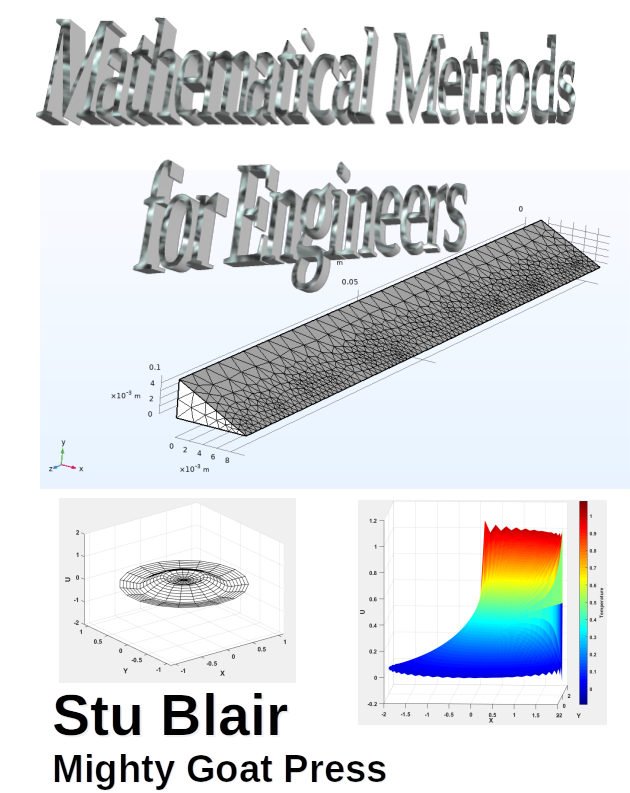
\includegraphics[width=1.5\textwidth]{cover1.png}
\end{figure}
\end{fullwidth}

% Front matter
\frontmatter

% r.1 blank page
%\blankpage


% v.2 epigraphs
\newpage\thispagestyle{empty}
\vfill
\openepigraph{%
When in doubt, multiply both sides by an orthogonal function and integrate.
}{P.L. Chebyshev}

\vfill
\openepigraph{%
The purpose of computing is insight, not pictures
}{L.N. Trefethen}


\vfill
\openepigraph{%
Never do a calculation until you already know the answer.
}{J.A. Wheeler}


% r.3 full title page
\maketitle


% v.4 copyright page
\newpage
\begin{fullwidth}
~\vfill
\thispagestyle{empty}
\setlength{\parindent}{0pt}
\setlength{\parskip}{\baselineskip}
Copyright \copyright\ \the\year\ \thanklessauthor
\par\smallcaps{Published by \thanklesspublisher}

%\par\smallcaps{tufte-latex.github.io/tufte-latex/}
%
%\par Licensed under the Apache License, Version 2.0 (the ``License''); you may not
%use this file except in compliance with the License. You may obtain a copy
%of the License at \url{http://www.apache.org/licenses/LICENSE-2.0}. Unless
%required by applicable law or agreed to in writing, software distributed
%under the License is distributed on an \smallcaps{``AS IS'' BASIS, WITHOUT
%WARRANTIES OR CONDITIONS OF ANY KIND}, either express or implied. See the
%License for the specific language governing permissions and limitations
%under the License.\index{license}

\par\textit{First printing, \monthyear}
\end{fullwidth}

% r.5 contents
\tableofcontents

\listoffigures

\listoftables

% r.7 dedication
%\cleardoublepage
%~\vfill
%\begin{doublespace}
%\noindent\fontsize{18}{22}\selectfont\itshape
%\nohyphenation
%Dedicated to the midshipmen of the United States Naval Academy; the future of our armed services and of %our country.
%\end{doublespace}
%\vfill
%\vfill


% r.9 introduction
\cleardoublepage
\chapter*{Preface}

The purpose of this text is to provide a concise reference for engineering students who would like to strengthen their conceptual understanding and practical proficiency in analytical and numerical methods in engineering.  The material is based on a sequence of two courses taught at the United States Naval Academy.  

\subsection*{Analytical Methods}

The first course focused on analytical methods for linear ordinary and partial differential equations.  All students came into the course having taken a three-semester sequence of calculus along with a course in ordinary differential equations.  The analytical methods portion quickly reviews methods for constant coefficient linear equations and proceeds to methods for non-constant coefficients including Cauchy-Euler equations, power series methods, and method of Frobenieus.  After a review of Fourier Series methods and an introduction to Fourier-Legendre and Fourier-Bessel expansions we thoroughly explore solutions to second-order, linear, partial differential equations.  Since many students are also studying nuclear engineering, there is a heavy focus on addressing boundary value problems in cylindrical and spherical coordinate systems that are applicable to other topics of interest such as reactor physics.  There is also heavy emphasis on heat transfer applications that students will see later on in their undergraduate curriculum.

The materials presented are based heavily on Professor Dennis Zill's excellent book.\cite[-3cm]{zill2020advanced} We lightly select from chapters 1-3 for review; chapter 5 for series solution methods; and chapters 12-14 for Fourier Series and solutions to linear boundary value problems.  Material from that text is used throughout this book.  

What distinguishes this course from Prof Zill's work is the incorporation of computational tools in the solution process.  These ``semi-analytical methods'' are presented here in MATLAB\cite[-3.75cm]{matlab} owing to the students preparation with that tool.  Other open-source tools like Octave\cite[-3.5cm]{octave} and Python,\cite[-1cm]{10.5555/1593511} of course, could be used. 

\subsection*{Numerical Methods}

%%
% Start the main matter (normal chapters)
\mainmatter

\part{Introduction and Review}

\chapter{Lecture 1 - Course Introduction and Numeric Preliminaries}
\label{ch:lec1n}
\section{Objectives}
The objectives of this lecture are:
\begin{itemize}
\item Introduce the course objectives.
\item Describe how numbers are represented on computers.
\item Outline sources of errors in numerical methods relative to analytical methods.
\end{itemize}
\setcounter{lstannotation}{0}

\section{Course Introduction}

This course is intended to be an introduction and overview of numerical methods.\marginnote[-0.5cm]{\textbf{Question:} What are numerical methods? 

\vspace{0.25cm}

\noindent \textbf{Answer:} Numerical methods (or numerical analysis) is the study of \emph{algorithms} for the problems of \emph{continuous} mathematics.}  The target audience comprises undergraduate students of engineering who have already taken a full sequence of calculus and differential equations courses.  Some students may also have taken the analytical methods course described earlier in this book. All students are expected to have some proficiency in the MATLAB programming environment.  

\subsection{Objectives}
\newthought{The objectives} for this course are as follows:

\begin{enumerate}
\item Students will understand the fundamentals of numerical methods with an emphasis on the most essential algorithms and methods.

\item Students will have enhanced their scientific computing skills and further developed their proficiency in using the MATLAB environment to implement algorithms and have learned to critically evaluate their results.

\item Students will understand the fundamentals of the finite element method (FEM) and have attained an introductory-level proficiency in using the COMSOL software package to carry out a multi-physics analysis of a relevant physical model.

\item Students will have developed the ability to formulate a problem of interest, apply numerical methods and computational tools to analyze the problem, and communicate pertinent results to others.
\end{enumerate}


\subsection{Course Topics}
The specific topics we will cover include:

\begin{enumerate}
\item Methods for solving non-linear equations
\begin{enumerate}
\item Bisection method
\item Newton's method
\item Secant method

\end{enumerate}
\item Methods for solving linear equations
\begin{enumerate}
\item Gauss elimination and related methods like LU- and Cholesky factorization
\item Iterative solution methods for sparse linear systems of equations\sidenote{We will also discuss some preconditioners.}
\end{enumerate}
\item Curve fitting
\begin{enumerate}
\item Least squares algorithms
\item Curve fitting with Lagrange polynomials
\end{enumerate}
\item Numeric differentiation
\begin{enumerate}
\item Finite difference methods
\item Lagrange polynomials
\end{enumerate}
\item Numeric integration
\begin{enumerate}
\item A variety of Newton-Cotes methods
\item Gauss Quadrature
\end{enumerate}

\item Initial- and Boundary-value problems \sidenote{This section will prominently include MATLAB built-in methods; particularly for boundary value problems.}
\begin{enumerate}
\item Runge-Kutta methods for initial value problems\sidenote{We will not extensively cover either explicit or implicit multi-step methods, giving preference to the wide variety of very effective RK methods.}
\item Shooting method for boundary value problems
\item Finite element method\sidenote{There will be a simple MATLAB demonstration with application to one-dimensional boundary value problems.  The majority of FEM coverage will be related to the use of COMSOL.}
\end{enumerate}

\end{enumerate}  

\vspace{4.0cm}

\section{Representation of Numbers on a Computer}

Every engineer who uses computational tools in their work should have a basic understanding of how numbers are represented on a computer.  The essential take-aways from this section are:
\begin{enumerate}
\item Since the computer is a finite machine, only a finite set of numbers can be exactly represented on the computer.  All other numbers are approximated.
\item Computers store integers and non-integers differently and the limits to what numbers can be represented or how exactly they are represented are also different.
\item The fact that numbers, in general, are represented inexactly on the computer has an impact on how algorithms are developed.
\end{enumerate}

\subsection{Integers}
Integers are represented exactly on a computer, but only a finite subset of all integers can be represented.  There are a number of integer types that are supported by common computer architectures and language compilers.\marginnote[-4.5cm]{Some of the integer data types specified by the C++ language standard include:
\begin{enumerate}
\item signed char (8 bits)
\item short int (16 bits)
\item int (at least 16 bits -- usually 32 bits)
\item long int (at least 32 bits)
\item long long int (at least 64 bits)
\end{enumerate}
Each of these categories includes a signed and unsigned variant.  Even within these categories there is fuzziness---e.g. \emph{``at least 16 bits''}---that allows for variations between different compiler implementations and computer hardware (e.g. Intel vs. AMD CPU).
}\marginnote{\textbf{Note:} The word \emph{bit} is taken to be synonymous with the words \emph{binary digit}.} For the purposes of this class we will focus on two types: \emph{unsigned integers} and \emph{signed integers}.  To further focus the discussion we will only consider 32-bit representations of signed and unsigned integers.

\newthought{Perhaps the easiest} integer representation to understand is the 32-bit unsigned integer.\sidenote{You can create a 32-bit unsigned integer in MATLAB by typing:

\vspace{0.1cm}

\noindent \lstinline[style=myMatlab]{x = uint32(1994)}

\vspace{0.1cm}

Variables with other data types can be constructed using similar syntax; see the MATLAB documentation for details.
} In this format 32 binary digits corresponding to $2^0$ to $2^{31}$ are stored in memory.  Numbers in binary work the same way our normal decimal number work: just base 2 instead of base 10.  For example, the 32-bit unsigned integer representation of the number 23 is shown in Figure \ref{fig:lec1n-binary-23}.


\begin{figure}[h!]
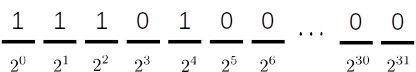
\includegraphics[width=0.75\columnwidth]{binary_23.png}
\caption{The number 23 in unsigned integer format.}
\label{fig:lec1n-binary-23}
\end{figure}


%\vspace{0.25cm}
%\noindent (image of 24 in binary)
%\vspace{0.25cm}

With 32-bit unsigned integers the computer can exactly represent all integers between 0 and $2^{32}-1$. Negative integers and integers greater than $2^{31}$ are not represented at all.%\sidenote{\textbf{Question:} What do you get from the following MATLAB code?
%\begin{lstlisting}[style=myMatlab]
%a = uint32(2^32-1);
%b = uint32(1);
%c = a + b;
%fprintf('c = %d \n',c);
%\end{lstlisting}

%\lstinline[style=myMatlab]{ a = uint32(2^32 - 1)  b = unit32(1) }

%\vspace{0.1cm}

%\noindent\textbf{Answer:} The variable c will still be equal to $2^{31}-1$.  MATLAB will round numbers outside of the range of representation for 32-bit unsigned ints to the nearest endpoint which, in this case, is $2^{31}-1$.
%}

\newthought{There are fewer} applications for which \emph{signed integers} will be used for this course, but they are, naturally, important.  Perhaps the most obvious way that a computer might represent signed integers would be to just use the same format as unsigned integers except to reserve one bit for the sign.  This is not, however, the way it is normally done.  For one thing, this approach results in there being two different bit-patterns for zero.  This might seem like a trivial inconvenience but it is not the sort of thing that passes without notice in computer engineering circles. Another, perhaps more significant, issue with this approach is that special logic would be needed when adding or subtracting a mixture of positive and negative integers. (i.e. you would not be able to use the same circuitry on the microprocessor for adding positive and negative numbers together as you would for adding two positive numbers.)
  
The format that is normally used today for representing signed integers is called \emph{two's complement}.  If you want to write a positive number in two's complement format, you do the same thing as you would normally do for an unsigned integer.\sidenote[][-1.5cm]{Except, as it turns out, the largest positive 32-bit signed integer will only half as large as the corresponding largest signed integer.} If you need to write a negative number, you start by expressing the positive number, then you \emph{take the complement of each binary digit} and, when you are done with that, you \emph{add one.} A demonstration of this number representation, shortened to 5-bits to make it more compact, is shown in Figure \ref{fig:twos-complement-demo}.  


\begin{marginfigure}
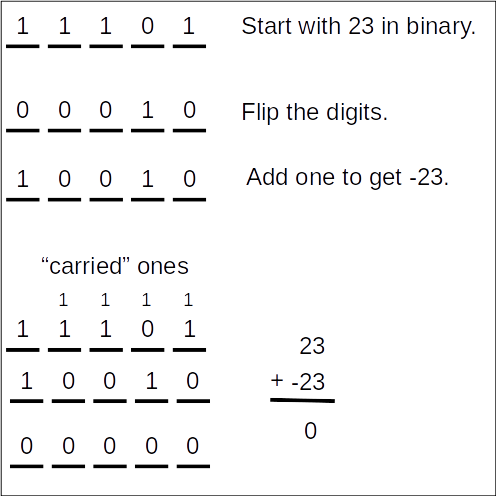
\includegraphics{twos-complement-demo.png}
\caption{Demonstration of twos-complement: adding 23 and -23 in 5-bit representation.}
\label{fig:twos-complement-demo}
\end{marginfigure}

%\vspace{0.25cm}
%\noindent (image showing example two's complement)
%\vspace{0.25cm}

This representation has the advantages that: a) there is only a single representation for zero; and b) the same hardware is used for both addition and subtraction (i.e. to subtract you simply add a negative number.)

\subsection{Floating Point Numbers}
In general, binary floating point numbers are given in the form shown in Equation \ref{eq:bfpn-format}:
\begin{equation}
1.\underbrace{\text{fff}\dots\text{f}}_{\text{mantissa}} \times 2^{\underbrace{\text{eee}\dots\text{e}}_{\text{exponent}}}
\label{eq:bfpn-format}
\end{equation}
where a number of digits available are divided between the fraction, or \emph{mantissa}, and \emph{exponent}.  In any finite machine, there will be a limit to the number of total digits available.  Thus an engineering decision needs to be made to determine how many digits will be allocated to the mantissa and how many for the exponent.  If you have more digits in the mantissa, you will be able to represent numbers that are closer together---the \emph{precision} of your representation will increase.  If you allocate more digits to the exponent, you will be able to represent numbers that are larger (for large positive exponents) or smaller (large negative exponents)---the \emph{range} of your representation will be wider.  The implications of these decisions should be clear: if you devote fewer bits to the mantissa, there will be more rounding errors in your calculations as real numbers are mapped, in some way, to the best floating point representation; if you devote fewer bits to the exponent, really large numbers and really small numbers will not be represented at all.  In earlier days of computing, different computer vendors made different decisions as to how floating point numbers would be represented.\cite{moler_fp1}  This caused problems when scientists tried to run the same code on different computers and got different results.  In 1985, the IEEE-754 standard was approved and, since then, has been adopted by essentially all computer manufacturers.  As a result, the menagerie of floating point formats and implementations have been tamed. Scientists and engineers could run their codes on different machines and expect to get the same results.

\begin{figure}
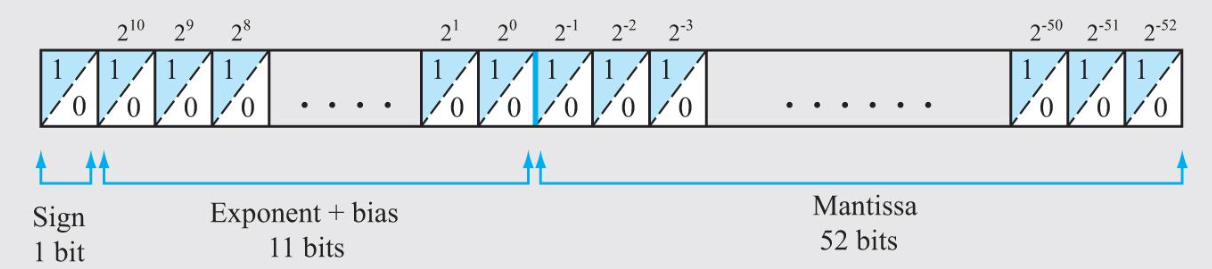
\includegraphics[width=0.94\columnwidth]{double-precision-format.png}
\caption{IEEE-754 double precision number format.}
\label{fig:double-precision-format}
\end{figure}

The IEEE-754 standard provides specification of several floating point number formats.  For this class, we will be concerned primarily with the \emph{double precision} floating point format which is illustrated in Figure \ref{fig:double-precision-format}.  This format uses a single sign bit (1 for negative, 0 for positive), 11 bits for the exponent which is encoded as an unsigned integer with bias,\sidenote{For double precision numbers, the bias is 1023.} and 52 bits for the mantissa.\sidenote{\textbf{Note:} The number 1 shown in Equation \ref{eq:bfpn-format} is not stored but is implicitly included in all \emph{normalized} floating point numbers.  This is done so that all numbers will have a \emph{unique} floating point representation. }  In the double precision format, the smallest positive number that can be represented is $2^{-1022}$ which is approximately equal to $2.2 \times 10^{-308}$.\marginnote{MATLAB includes built-in functions to report the smallest and largest representable floating point numbers.  The functions \lstinline[style=myMatlab]{realmin(precision)} and \lstinline[style=myMatlab]{realmax(precision)} will return the  smallest or largest positive floating point number for ``single'' or ``double'' precision floating point precision.} The smallest interval between numbers that can be represented is called \emph{machine epsilon}.\marginnote{In MATLAB, machine epsilon is provided with the function: \lstinline[style=myMatlab]{eps(precision)} for ``single'' and ``double'' precision.}  The size of this limit is driven by the number of bits in the mantissa.  For IEEE-754 double precision floating point numbers this is approximately $2.22 \times 10^{-16}$.\sidenote{Sometimes computational scientists refer to this as ``16 digits of precision.''}

\newthought{The procedure to} encode real numbers in the double precision floating point format will be illustrated with an example.

\vspace{0.5cm}

\noindent\textbf{Example:} Write the number -10.5 using the IEEE-754 double precision format.

\vspace{0.25cm}

\noindent\textbf{Step \#1:} Determine the mantissa and the exponent.  To do this, we normalize the number by dividing by $2^e$ where $e$ is the largest power of 2 that is \emph{less} than the magnitude of the number you are encoding.  

\vspace{0.1cm} 

\noindent In this case, $e=3$ since 10.5 is greater than $2^3$ but less than $2^4$.  

\begin{align*}
\frac{-10.5}{2^3} & = -1.3125 \\
\Rightarrow -10.5 &= -1.3125 \times 2^3
\end{align*}

\noindent Therefore the mantissa will need to encode 0.3215, and the exponent will need to encode 3 plus the bias of 1023, or 1026.

\vspace{0.25cm}

\noindent\textbf{Step \#2:} Set the sign bit. As the number is negative, the sign bit is: 1.

\vspace{0.25cm}


\noindent\textbf{Step \#3:} Calculate the 11 exponent bits.  

\begin{align*}
1026 &= 1024 + 2 \\
&= 1 \times 2^{10} + 1 \times 2^{1}
\end{align*}


\begin{figure}
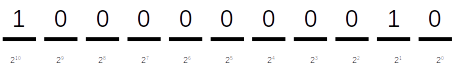
\includegraphics[width=0.75\columnwidth]{lec1n-ex1-exponent.png}
\caption{Exponent: 3+1023 = 1026 in 11-bit binary.}
\label{fig:lec1n-ex1-exponent}
\end{figure}   
  

\vspace{0.25cm}

\noindent\textbf{Step \#4:} Calculate the 52 mantissa bits to represent 0.3125.  The result is shown in Figure \ref{fig:lec1n-ex1-mantissa}.

\begin{figure}
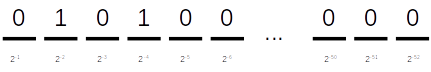
\includegraphics[width=0.75\columnwidth]{lec1n-ex1-mantissa.png}
\caption{Mantissa: 0.25 + 0.0625 = 0.3125.}
\label{fig:lec1n-ex1-mantissa}
\end{figure}

\noindent Where the calculations might be done as shown below:
\begin{align*}
0.3125 - 0 \times 2^{-1} &= 0.3125 \\
0.3125 - 1 \times 2^{-2} &= 0.0625 \\
0.0625 - 0 \times 2^{-3} &= 0.0625 \\
0.0625 - 1 \times 2^{-4} &= 0
\end{align*}
and all other entries are, of course, zero.


\section{Sources of Error} \index{error, truncation} \index{error, round-off} \index{error, modeling}

When using numerical methods there are several sources of error that you, as an engineer, should be aware of.  We have just discussed the details of double precision numbers so \emph{round-off error} is at the top of our mind.  Real numbers are not represented exactly on a computer but instead as floating point numbers.  The floating point number \emph{closest} to the real number gets used in its place. Error due to this round-off accumulates with mathematical operations.  Quantitative analysis of the accumulation of round-off-error is a tedious (albeit important) business that we will avoid in this class.  Nonetheless, engineers need to be aware that it is happening and, in a few instances, we will take steps to mitigate this build-up of error.

The second source of error that we will mention here is something that should be familiar to students who have taken the course in analytical methods: \emph{truncation error}.  In the analytical methods course we suffered from truncation error every time we shortened our infinite series solution to a finite number of terms.  We reduced this error by increasing the number of terms we retained, but there was no way to make it go away completely.  In this course we will see further instances of truncation error in most every algorithm we implement.  Derivatives and integrals that could, in principle, be done exactly, will be done approximately as we truncate the Taylor series expansion or limit the order of polynomials used to represent the exact derivative or integral.  We can reduce the magnitude of these errors, but we cannot make them go away entirely.

The third source of error mentioned here is \emph{modeling error}.  Modeling errors are reflected in the differences between observed physical phenomena and the corresponding mathematical model of the phenomena.  There are a couple of reasons for these differences and these include:
\begin{enumerate}
\item Linearization of non-linear processes.  Instances where you may already have done this, in your heat transfer or fluid dynamics class, include:
\begin{enumerate}
\item Assumption of constant thermal conductivity for heat conduction problems.  This assumption linearizes the heat equation and, for simple geometry, renders the problem amenable to analytical methods.  This assumption is retained for many numerical methods when solving the heat equation on more complex geometry.  The modeling error resulting from linearization remains.

\item Assumption of constant drag coefficient for external flow calculations.  Once again, this assumption simplifies the calculations at the cost of model fidelity.
\end{enumerate}

\item De-coupling of physical processes.  Nature does not specialize its behavior by academic subjects.  Consequently the air flowing over the control surfaces of a fighter jet is both a fluid dynamics and structural dynamics problem when the wing responds to forces imposed by the air.  Water flowing through a pressurized water reactor core is heated by forced convection and radiation that you might calculate in heat transfer class, but the resulting change in water properties also affect the neutron economy and power production rate that you might calculate in reactor physics which, in turn, will have further effect on the heat transfer problem.  We de-couple these processes so the analysis is more manageable but as a result the solution we arrive at is in error.  

\end{enumerate}  
Scientists and engineers need to be aware of all of these sources of errors and take steps to mitigate them where possible.




\chapter{Lecture 2 - Separable and Linear 1st order Equations}
\label{ch:lec2}
\section{Objectives}
The objectives of this lecture are:
\begin{itemize}
\item Define and describe the solution procedure for \emph{separable} first order equations
\item Define and demonstrate the solution procedure for \emph{linear} first order equations
\end{itemize}

\section{Separable Equations}
A first order differential equation of the form shown below
\begin{equation}
\frac{du}{dx} = g(u)h(x)
\label{eq:separable}
\end{equation}
is said to be \emph{separable} or have \emph{separable variables.}\marginnote[-1.5cm]{\textbf{Note:} there is \textbf{no} requirement that the 1st order equation be \emph{linear}.  This is one of the few techniques that we will study in this course that can be applied to nonlinear equations.} 

\newthought{The solution method} for separable equations is, in princple simple.  For the separable differential equation given in Equation \ref{eq:separable} we would separate and integrate:

\begin{align*}
\frac{du}{dx} &= g(u)h(x) \\
\frac{du}{g(u)} &= h(x) dx \\
\int \frac{1}{g(u)} \ du &= \int h(x) \ dx 
\end{align*}
\marginnote[-3.5cm]{\textbf{Note:} there are at least two complications here.
\begin{enumerate}
\item The solution you thus derive may be either implicit or explicit.  An implicit solution is, as a practical matter, fairly inconvenient to deal with; and
\item It may not be possible to actually carry out the integrals analytically. 
\end{enumerate}
Nonetheless, we shall carry on and give it a try anyway.  
}
Generally speaking, one of your first checks for a first order equation should be: is it separable?  If so, you should separate the variables and solve.  The examples below are intended to illustrate the method.  Note that in the final example, the integral cannot be done analytically.
\begin{example}[h!]
Solve the following separable, first order differential equations
.
\textbf{Example 1:} 
\begin{align*}
\frac{du}{dx} &= \frac{u}{1 + x} \\
\frac{du}{u} &= \frac{dx}{1+x} \\
\int \frac{d}{u} &= \int \frac{dx}{1+x} \\
\ln{|u|} + c_1 &= \ln{|1+x|} + c_2 \\
|u| &= e^{\left[\ln{|1+x|} + c_3\right]}\\
    u(x)&= c|1+x|
\end{align*}

\end{example}

\begin{example}[h!]
\textbf{Example 2:}
\begin{align*}
\frac{du}{dx} &= -\frac{x}{u} \\
\int u \ du &= -\int x \ dx \\
\frac{u^2}{2} &= -\frac{x^2}{2}+c \\
u(x) &= \sqrt{c - x^2}
\end{align*}
\end{example}

\begin{example}[h!]
\textbf{Example 3:}
Solve the first order initial value problem shown below:
\begin{equation}
\frac{du}{dx} = e^{-x^2}, \ \ u(2) = 6, \ \ 2 \le x < \infty
\end{equation}
\begin{align*}
du &= e^{-x^2}\ dx \\
\int_2^{x} \frac{du}{dt} \ dt &= \int_{2}^{x} e^{-t^2} \ dt \\
u(x) - u(2) &= \int_{2}^{x} e^{-t^2} \ dt \\
u(x) &= 6 + \int_{2}^{x} e^{-t^2} \ dt
\end{align*}
where we have used the dummy variable $t$ in the integrals; the last integral will need to be evaluated numerically.

\end{example}

\section{Linear Equations}
A first-order differential equation of the form:
\begin{equation}
a_1(x)\frac{du}{dx} + a_0(x)u = g(x)
\label{eq:lin_first_order}
\end{equation}
is said to be a first order \emph{linear equation} in the dependent variable $u$.\marginnote[-2.0cm]{\textbf{Note:} it is sometimes customary to write the differential equation in \emph{operator form} where the differential operator, $\mathcal{L}=a_1(x) \frac{d}{dx} + a_0(x)$, is applied to the function $u(x)$ to get $g(x)$; $\mathcal{L}u(x) = g(x)$ }
When $g(x) = 0$, the first-order linear equation is said to be \emph{homogeneous}; otherwise it is \emph{nonhomogeneous}.\marginnote{Notice that $g(x)$ is the only term in Equation \ref{eq:lin_first_order} that does \underline{\textbf{not}} include $u$ or any of its derivatives.}

\newthought{When solving} equations of this type it is useful to express it in the \textbf{standard form}:
\begin{equation}
\frac{du}{dx}+P(x)u = f(x)
\label{eq:first-order-linear-standard-form}
\end{equation}  
The method for solving this equation makes use of the \underline{\emph{linearity}} property\marginnote{When we say an operator is \textbf{linear}, what we mean is that the following relationships must hold:
\begin{enumerate}
\item $\mathcal{L}(\alpha u) = \alpha \mathcal{L}(u)$
\item $\mathcal{L}(u + v) = \mathcal{L}(u) + \mathcal{L}(v)$
\end{enumerate}
for functions $u$,$v$ and scalar constant $\alpha$.  Think of this as a \emph{definition} of linearity.} and express the solution in the following way: $u(x) = u_c(x) + u_p(x)$; plugging this into Equation \ref{eq:first-order-linear-standard-form} gives us:

\begin{multline}
\frac{d}{dx}[u_c + u_p] + P(x)[u_c + u_p] = \\
\left[\frac{du_c}{dx}+P(x)u_c \right] + \left[\frac{du_p}{dx}+P(x)u_p \right] = f(x) 
\label{eq:lin-first-order1}
\end{multline}
where $u_c(x)$ is the solution to the \emph{associated homogeneous problem}\marginnote{The linear operator here is: $\mathcal{L}=\frac{d}{dx} + P(x)$.  Equation \ref{eq:fol_complementary} says $\mathcal{L}u_c = 0$; Equation \ref{eq:fol_particular} says $\mathcal{L}u_p = f(x)$; Equation \ref{eq:lin-first-order1} says that $\mathcal{L}(u_c+u_p) = 0+f(x) = f(x)$.}
\marginnote[0.25cm]{What might trouble you now is: if we have $u_p$, is this not a solution to Equation \ref{eq:first-order-linear-standard-form}?  Why do we need $u_c$?  The next thing that should trouble you is that if $u_p$ is a solution, by the linearity property of $\mathcal{L}$, so is $u_p$ plus \emph{any} constant multiple of $u_c$.  The solution is not \emph{unique}}
\marginnote[0.25cm]{This will all be resolved when we recall that $u_c$ will have an arbitrary constant through which we will be able to say that $u = u_c + u_p$ is a function describing \emph{all} possible solutions of Equation \ref{eq:first-order-linear-standard-form} and the arbitrary constant in $u_c$ will be set so as to uniquely satisfy a given initial/boundary condition.}
\begin{equation}
\frac{du_c}{dx}+P(x)u_c = 0
\label{eq:fol_complementary}
\end{equation}
and $u_p(x)$ is the solution to:
\begin{equation}
\frac{du_p}{dx}+P(x)u_p = f(x)
\label{eq:fol_particular}
\end{equation}
We can see that Equation \ref{eq:fol_complementary} is separable:
\begin{align*}
\frac{du_c}{dx}+P(x)u_c &= 0 \\
\frac{du_c}{u_c} &= -P(x) \ dx \\
\ln{u_c} + C &= -\int_{P(x) \ dx} \\
u_c(x) &= e^{-\int P(x) \ dx + C_1} \\
u_c(x) &= e^{-\int P(x) \ dx}e^{C_1}
u_c(x) &=Ce^{-\int P(x) \ dx}
\end{align*}
where $C = e^{C_1}$.\marginnote{\textbf{Note:} At some point in time, I will desist in making such piddling distinctions between constants.  $C_1$ is an arbitrary constant, $e^{C_1}$ is still an arbitrary constant; there is no real difference between $C_1$ and $C$ and, in this author's humble opinion, they do not rate different symbols.}

\newthought{We need to find} a solution $u_p(x)$ to Equation \ref{eq:fol_particular}.  The technique we will use is called \emph{variation of parameters}.  It consists of looking for a solution in the form $y_p(x) = v(x)u_1(x)$, where $u_1(x) = e^{-\int P(x) \ dx}$ which is $u_c(x)$ with the arbitrary constant set to 1 and $v(x)$ might be thought of as some kind of weighting or \emph{variational} function.

\newthought{We will insert} this proposed form of $y_p(x)$ into Equation \ref{eq:fol_particular}:
\begin{equation*}
\frac{d(vu_1)}{dx} + P(x)(v(x)u_1(x))=f(x)
\end{equation*}
We apply the product rule to the first term and re-arrange terms:
\begin{align*}
u_1(x)\frac{dv}{dx}+ v(x)\frac{du_1}{dx} + P(x)(v(x)u_1(x)) &= f(x) \\
v(x)\underbrace{\left[\frac{du_1}{dx}+P(x)u_1(x) \right]}_{\textbf{= 0}}+u_1(x)\frac{dv}{dx} &= f(x) \\
u_1(x)\frac{dv}{dx} &= f(x)
\end{align*}
In the last line we can observe that the equation is \emph{separable} and thus solve:
\begin{align*}
v(x) &= \int \frac{f(x)}{u_1(x)} \ dx \\
     &= \int e^{\int P(x) \ dx}f(x) \ dx
\end{align*}
Now that we know what $v(x)$ must be, we can combine this with $u_1(x)$ to get $u_p(x)$:
\begin{equation}
u_p(x) = e^{-\int P(x) \ dx}\left[\int e^{\int P(x) \ dx}f(x) \ dx \right]
\label{eq:fol-particular-sol}
\end{equation}
Equation \ref{eq:fol-particular-sol} is messy and perhaps a bit scary but given definitions of $P(x)$ and $f(x)$ we might hope we can solve it anyway.  We now have expressions for both $u_c$ and $u_p$; they can be combined into the solution for the first-order linear equation:
\begin{equation}
u(x) = Ce^{-\int P(x) \ dx} + e^{-\int P(x) \ dx} \left[e^{\int P(x) \ dx} f(x) \ dx \right]
\label{eq:fol-solution}
\end{equation}

\section{Method of Solution}
Once we have identified a problem to be first-order and linear, we will solve the problem using the following steps:
\begin{enumerate}
\item Write the equation in standard form (Equation \ref{eq:first-order-linear-standard-form})
\item Determine the integrating factor $\mu = e^{-\int P(x) \ dx}$.
\item Solve for the general solution $u(x)$ using Equation \ref{eq:fol-solution}.
\item Apply initial/boundary condition if given.
\end{enumerate}

\vspace{1cm}
\underline{\textbf{Example:}}
Solve the problem:
$$\frac{du}{dx}+u=x, \ \ u(0) = 4$$

\textbf{Solution:}

\textbf{Step 1:}
The equation is already in standard form, so this step is easy.

\vspace{0.25cm}
\textbf{Step 2:} Find the integrating factor $\mu$.

$$mu = e^{-\int P(x) \ dx} = e^{-\int 1 \ dx} = e^{-x}$$

\vspace{0.25cm}
\textbf{Step 3:} Solve for the general solution $u(x)$ using Equation \ref{eq:fol-solution}
\marginnote[1.25cm]{$\leftarrow$ For the integral $\int e^x x \ dx$ we need to use integration by parts.}
\begin{align*}
u(x) &= Ce^{-x}+e^{-x}\int e^{x}x \ dx \\
&= Ce^{-x} + e^{-x}\left[xe^{x}-e^{x} \right] \\
&= Ce^{-x} + x - 1
\end{align*}

\vspace{0.25cm}
\textbf{Step 4:} Apply initial/boundary conditions if given

\begin{align*}
u(0) &= Ce^{0} + 0 -1 \\
 &=C-1 = 4 \\
 \Rightarrow C &= 5 \\
 u(x) &= 5e^x+x-1
\end{align*}




\chapter{Assignment \#1}
\label{ch:ass1n}
\begin{fullwidth}

\begin{enumerate}
\item Write the number 38.8125 as a 64-bit double-precision string using the IEEE-754 standard. 



\vspace{2.0cm}

\item In single precision (IEEE-754 standard), 8 bits are used for storing the exponent (the bias is 127), and 23 bits are used for storing the mantissa.  What (approximately) are the smallest and largest positive numbers that can be stored in single precision?

\vspace{2.0cm}

\item The value of $\pi$ can be calculated with the series:
\begin{equation*}
\pi = 4 \sum\limits_{n=1}^{\infty} (-1)^{n-1}\frac{1}{2n-1} = 4 \left(1 - \frac{1}{3} + \frac{1}{5} - \frac{1}{7} + \frac{1}{9} - \frac{1}{11} + \cdots \right)
\end{equation*}
Write a MATLAB script that calculates the value of $\pi$ by using $n$ terms of the series and calculate the corresponding true relative error.  Calculate $\pi$ and the true relative error for $n=10$, 20, and 40. \textbf{Note:} Implement the partial series summation as a \emph{local function} named \lstinline[style=myMatlab]{piApprox} that takes one argument---the number of terms ($n$)---and returns the estimated value of $\pi$ and the true relative error.  Use MATLAB's built-in constant \lstinline[style=myMatlab]{pi} for the ``true'' value of $\pi$.

\vspace{2.0cm}

\item Using a hand calculator, determine the root of $f(x)=x-2e^{-x}$ with the bisection method.  Start with $a=0$ and $b=1$, and carry out the first three iterations to determine an estimated root and bracket within which the root lies.

\vspace{2.0cm}

\item Write a MATLAB user-defined function that solves for a root of a nonlinear equation $f(x)=0$ using the bisection method.  Implement the function as a \emph{local function} that takes three arguments: \lstinline[style=myMatlab]{fun}, \lstinline[style=myMatlab]{a}, and \lstinline[style=myMatlab]{b}, where \lstinline[style=myMatlab]{fun} is a handle to the nonlinear function for which a root is to be found and \lstinline[style=myMatlab]{a} and \lstinline[style=myMatlab]{b} bracket the root.  The bisection iterations should stop when $f(x_{\text{NS}})\le 0.0000001$ where $x_{\text{NS}}$ is the midpoint of the current bracket.  The function should also check if points \lstinline[style=myMatlab]{a} and \lstinline[style=myMatlab]{b} do indeed bracket a root; if not, the function should return an error message.  Use your function to find the root of $f(x) = x-2e^{-x}$.  


\vspace{2.0cm}
\index{van der Waals equation}
\item The van der Waals equation gives a relationship between the pressure $P$ (in atm.), volume $V$ (in liters), and temperature $T$ (in K) for a real gas:
\begin{equation}
P = \frac{nRT}{V-nb}-\frac{n^2 a}{V^2}
\label{eq:ass1n-van-der-waals}
\end{equation}
where $n$ is the number of moles, $R=0.08206$ (L-atm)/(mole-K) is the gas constant, and $a$ (in L\textsuperscript{2}-atm/mole\textsuperscript{2}) and $b$ (in L/mole) are material constants.  Consider 1.5 moles of nitrogen ($a$=1.39 L\textsuperscript{2}-atm/mole\textsuperscript{2}) at 25$^{\circ}$C stored in a pressure vessel.  Use the function you created for problem \#5 to determine the volume of the vessel if the pressure is 13.5 atm.


\end{enumerate}

\end{fullwidth}

\chapter{Lecture 3 - Theory of Linear Equations}
\label{ch:lec3}
\section{Objectives}
The objectives of this lecture are:
\begin{itemize}
\item Introduce several theoretical concepts relevant to initial value problems and boundary value problems.
\item Demonstrate use of the Wronskian to determine linear independence of solutions.
\item Present some important theorems and definitions relevant to the theory of linear ordinary differential equations.
\end{itemize}

\section{Initial Value Problems}

For a linear differential equation, an n\textsuperscript{th}-order initial value problem (IVP) is given by the following governing equation and initial conditions:
\begin{equation}
\text{Governing Equation: }a_n(x)\frac{d^n u}{dx^n}+a_{n-1}\frac{d^{n-1}u}{dx^{n-1}}+\cdots+a_1(x)\frac{du}{dx}+a_0(x)u=g(x)
\label{eq:ivp-ge}
\end{equation}
\begin{equation}
\text{Initial Conditions: }u(x_0)=u_0, \ u^{\prime}(x_0)=u_1,\dots,u^{(n-1)}(x_0)=u_{n-1}
\label{eq:ivp-ics}
\end{equation}
\marginnote[-1.5cm]{\textbf{Note:} for an initial value problem, all of the initial conditions are provided at the same value of $x$; in accordance to custom we call this $x_0$.  The name \emph{initial} condition gives the implication that these conditions are at some ``end'' of the interval (beginning, left side, whatever) and in most all examples and exercises this is indeed the case.  It is \underline{not}, however, a requirement.}
\noindent \newthought{We seek a} function defined on some interval containing $x_0$ that satisfies the differential equation with $n$ conditions applied.\marginnote{Generally for an n\textsuperscript{th}-order IVP you will need $n$ conditions.} The theorem below, which we will use by \emph{citing} rather than \emph{proving}, gives us assurance that, subject some fairly reasonable assumptions, such a solution will exist.  

\begin{theorem}[Existence and Uniqueness for IVPs]
If $a_n(x),a_{n-1}(x),\dots,a_1(x),a_0(x)$ and $g(x)$ are continuous on an interval $\mathcal{I}$, and if $a_n(x) \ne 0$ for every $x \in \mathcal{I}$, and if $x_0$ is any point in this interval, then a solution $u(x)$ of the IVP exists on the interval and it is unique.
\label{thm:IVP-exist-and-unique}
\end{theorem}
\newthought{For this class} we will adopt a mostly operational definition of continuity: if you can draw the function throughout the specified interval without picking up your pencil or without diverging to infinity, then the function is continuous.  

Consider, as an example, the following initial value problem:
\begin{equation}
u^{\prime \prime}-4u = 12x, \ \ u(0)=4, \ u^{\prime}(0)=1
\end{equation}
This IVP satisfies the conditions of Theorem \ref{thm:IVP-exist-and-unique} since all of the coefficients and $g(x)$ are continuous and $a_1$ is constant and nonzero; hence a unique solution exists on any interval and that solution is unique.\marginnote[-1.5cm]{Take a moment to verify that $u(x)=3e^{2x}+e^{-2x}-3x$ satisfies both the governing equation and initial conditions and thus is \emph{the} unique solution to this IVP.}

Here is an IVP that does \emph{not} satisfy the criteria of Theorem \ref{thm:IVP-exist-and-unique}:
\begin{equation}
x^2u^{\prime \prime} - 2xu^{\prime}+2u=6, \ \ u(0)=3, \ u^{\prime}(0)=1
\label{eq:lec3-ex2}
\end{equation}
\noindent In this case, the coefficients and $g(x)$ are all continuous but $a_2(x)$ is equal to zero at $x=0$.  This might not be a problem---i.e. if $x=0$ is not in the interval of interest for the IVP then we are okay---but since $x_0=0$, $x=0$ \emph{must} be in the domain for the theorem to apply.  So we have no assurances that a solution exists or, if a solution does exist, it may not be unique.\marginnote[-1.5cm]{You should take a moment to verify that $u(x)=cx^2+x+3$ is a solution for the IVP given in Equation \ref{eq:lec3-ex2} for \emph{any} choice of parameter $c$.}

\section{Boundary Value Problems}
For this section let us, without undue loss of generality, consider a 2\textsuperscript{nd}-order boundary value problem (BVP):\marginnote{Almost all of the applications we will consider for this class will involve 2\textsuperscript{nd}-order operators.  The way we derive important boundary-value problems from underlying physical laws like conservation of mass and conservation of energy lead to them being 2\textsuperscript{nd}-order.  You should think about this while you are sitting in your fluid dynamics class and equations are being derived for conservation of mass and momentum for viscous incompressible fluid flow or when you are sitting in heat transfer class and the heat equation is being derived from conservation of energy principles.  Probably the most obvious counterexample is beam theory which involves a 4\textsuperscript{th}-order operator.}
\begin{equation}
\text{Governing Equation: }a_2(x)\frac{d^2u}{dx^2}+a_1(x)\frac{du}{dx}+a_0(x)u=g(x) 
\end{equation}
\begin{equation}
\text{Boundary Conditions: } y(a)=y_0, \ \ y(b)=y_1, \ \ a \ne b
\end{equation}

\newthought{Depending on the} boundary conditions, BVPs may have no solutions, one unique solution, or infinitely many solutions.

\vspace{1.0cm}
\noindent \underline{\textbf{Example:}} The equation $u^{\prime \prime}+16u = 0$ has the general solution $u(t) = c_1 \cos{(4t)}+c_2 \sin{(4t)}$.  Consider the three different sets of boundary conditions provided below.
\begin{enumerate}[label=\alph*)]
\item $x(0)=0, \ \ x(\pi/2)=0$
Application of the first boundary condition gives us $c_1(1)+c_2(0)=0 \Rightarrow c_1 = 0$.  The second boundary condition is $c_2\sin{(2 \pi)} = 0,$ which is true for \emph{any} value of $c_2$.  Therefore there problem has infinitely many solutions.
\item $x(0)=0, \ \ x(\pi/8)=0$
The first boundary condition again gives us $c_1=0$; the second condition $c_2\sin{(4 \frac{\pi}{8})}=0$ is only satisfied if $c_2=0$.  Thus $c_1 = c_2 = 0$; only the trivial solution, $u=0$, satisfies both the differential equation and boundary conditions.  This is not a very interesting solution but at least it \emph{is a solution} so we will take this as an example of a BVP having a unique solution.\marginnote{For applications, we will generally be only interested in \emph{non-trivial} solutions; that is, solutions that are not identically equal to zero.}
\item $x(0)=0, \ \ x(\pi/2)=1$
In this case, again $c_1=0$ from the first boundary condition.  This leaves the second boundary condition: $c_2 \sin{\left(4 \frac{\pi}{2}\right)} = c_2(0) = 1$ which cannot be satisfied for any value of $c_2$.  In this case \emph{no} solution exists.

\end{enumerate}

\section{Superposition and Linear Dependence}
In this section some important theorems regarding IVPs and BVPs will be presented.  No attempt will be made to prove these theorems; we will simply take these theorems as facts that are relevant for this course that you should try to understand as best you can.

\begin{theorem}[Superposition Principle for Homogeneous Equations]
Let $u_1,u_2,\dots,u_k$ be solutions of a homogeneous n\textsuperscript{th}-order linear differential equation.  Then any linear combination of those solutions 
$$u = c_1u_1+c_2u_2+\cdots+c_ku_k$$where $c_1,c_2,\dots,c_k$ are arbitrary constants, is also a solution.
\end{theorem}
\marginnote[-3.0cm]{\textbf{Note:} It is essential that \emph{both} the governing equation and given conditions (boundary or initial) for the linear differential equation are homogeneous.  As a reminder, this means that \emph{all} terms in the governing equation and boundary conditions must either a) involve the dependent variable or one of its derivatives; or b) be equal to zero.} 
As an example, If I denote the linear homogeneous differential equation as $\mathcal{L}$, then $\mathcal{L}(u_i) = 0$ for any $i \in [1,2,\dots,k]$.  By the linearity property of $\mathcal{L}$, for any constants $\alpha$ and $\beta$:
\begin{align*}
\mathcal{L}(\alpha u_i + \beta u_j) &=  \alpha \mathcal{L}(u_i) + \beta \mathcal{L}(u_j)\\
&= \alpha(0) + \beta(0) \\
&= 0
\end{align*}

\begin{theorem}[Linear Dependence / Independence of Functions]
A set of functions $f_1(x),f_2(x),\dots,f_k(x)$ is said to be \emph{linearly dependent} on an interval $\mathcal{I}$ if there exist constants $c_1,c_2,\dots,c_k$, \emph{not \underline{all} of which are zero}, such that
$$c_1f_1(x) + c_2f_2(x)+\cdots+c_kf_k(x) = 0$$
\noindent for every $x \in \mathcal{I}$.  If the set of functions is \emph{not} linearly dependent, it is linearly independent.
\label{th:linear-dep}
\end{theorem} 
\marginnote[-1.75cm]{What if a member of the set of functions is $f(x)=0$? 

\vspace{0.25cm}

\noindent\textbf{Answer:} The set will no longer be linearly independent.  The trivial function $f(x)=0$ is not linearly independent from \emph{anything}.}
Repeatedly throughout this course we will want to clarify whether or not two or more functions are linearly independent of each other.  I think most engineers have a general idea of what it is we \emph{mean} when we say two functions are linearly independent or dependent but Theorem \ref{th:linear-dep} specifies what these things mean \emph{mathematically}.  
\newthought{We need a test} to help us determine if the members of a set of functions are linearly independent or not. This will be especially important as we evaluate solutions to a linear homogeneous differential equation.  Even if you are the sort of savant who can, by inspection, always detect linear dependence, you might have a hard time convincing your friends that your assessment is always correct.  Luckily, there is a theorem that provides a suitable test that can serve as irrefutable evidence of the state of linear dependence/independence of functions.

\begin{theorem}[Criterion for Linearly Independent Solutions]
Let $u_1,u_2,\dots,u_n$ be solutions of a homogeneous linear n\textsuperscript{th}-order differential equation defined on an interval $\mathcal{I}$.  Then the set of solutions is linearly independent on the interval if and only if the Wronskian of the solution is non-zero for every $x \in \mathcal{I}$.  
\end{theorem}\index{Wronskian}
The Wronskian is a function that takes functions as arguments and returns a scalar numeric quantity.\sidenote{Sometimes such functions are referred to as \emph{functionals}.}
\begin{equation}
W(u_1,u_2,\dots,u_n)=
\begin{vmatrix}
u_1 & u_2 & \cdots & u_n \\
u^{\prime}_1 & u^{\prime}_2 & \cdots & u^{\prime}_n \\
\vdots & \vdots & \vdots & \vdots \\
u^{(n-1)}_1 & u^{(n-1)}_2 & \cdots & u^{(n-1)}_n
\end{vmatrix}
\label{eq:Wronskian-def}
\end{equation}
where $|\cdot|$ denotes the matrix determinant.  For large values of $n$ this is also difficult to calculate but, for the case $n=2$, engineering students should be familiar with the formula:
\begin{equation}
W(u_1,u_2) = 
\begin{vmatrix}
u_1 & u_2 \\
u^{\prime}_1 & u^{\prime}_2 \\
\end{vmatrix}
= u_1 u^{\prime}_2 - u^{\prime}_1 u_2
\end{equation}

\vspace{0.5cm}

\noindent\textbf{\underline{Example:}} show that the functions $u_1 = e^{3x}$ and $u_2=e^{-3x}$ are linearly independent solutions to the homogeneous linear equation $u^{\prime \prime}-9u=0$ for every $x \in (-\infty,\infty)$.

\noindent\textbf{\underline{Solution:}} The Wronskian is given by:\marginnote{The reader should verify that both $u_1 = e^{3x}$ and $u_2=e^{-3x}$ satisfy the given differential equation.}
\begin{align*}
W &= 
\begin{vmatrix}
e^{3x} & e^{-3x} \\
3e^{3x} & -3e^{-3x}
\end{vmatrix} \\
&= e^{3x}\left(-3e^{-3x}\right) - 3e^{3x}\left(e^{-3x}\right) \\
&= 3e^{3x-3x} - 3e^{3x-3x} \\
&= 3 - 3 \\
&= 6
\end{align*}
\noindent Since $6 \ne 0$ for all $x \in (-\infty,\infty)$ the solutions are linearly independent.

\begin{definition}[Fundamental Set of Solutions]
Any set $u_1,u_2,\dots,u_n$ of $n$ linearly independent solutions of the homogeneous linear n\textsuperscript{th}-order differential equation on an interval is said to be a fundamental set of solutions on an interval $\mathcal{I}$.  
\end{definition}
\begin{theorem}[Existence of a Fundamental Set]
There exists a fundamental set of solutions for the homogeneous linear n\textsuperscript{th}-order differential equation on an interval $\mathcal{I}$.
\end{theorem}
\marginnote[-1.0cm]{\textbf{Note:} This is different than saying that a BVP or IVP has a solution.  This theorem is only referring to the differential equation; not the boundary or initial conditions.}

\begin{definition}[General Solution---Homogeneous Equation]
Let $u_1,u_2,\dots,u_n$ be a fundamental set of solutions to the homogeneous linear n\textsuperscript{th}-order differential equation defined on an interval $\mathcal{I}$, then the general solution is:
$$u(x) = c_1u_1(x)+c_2u_2(x)+\cdots+c_nu_n(x)$$
\end{definition}

\newthought{It is important} to understand from the above that:
\begin{itemize}
\item \emph{any} possible solution to the homogeneous, linear, n\textsuperscript{th}-order differential equation can be constructed by setting the coefficients of the general solution; and
\item there is \textbf{no} solution that can be constructed from functions that are linearly independent from the general solution.
\end{itemize}

\section{General Solution for a Non-homogeneous Problem}
Recall: ``non-homogeneous'' for a linear n\textsuperscript{th}-order differential equation means that $g(x)\ne 0$.  if $u_p$ is any particular solution to the non-homogeneous, linear, n\textsuperscript{th}-order ODE on an interval $\mathcal{I}$ and $u_c = c_1u_1(x) + c_2u_2(x)+\cdots c_nu_n(x)$ is the general solution to the associated homogeneous ODE (called the \emph{complementary} solution) then the general solution to the non-homogeneous ODE is:
\begin{equation*}
u = u_c + u_p
\end{equation*}

\vspace{0.25cm}

\noindent\textbf{\underline{Example:}} By substitution it can be seen that $u_p = -\frac{11}{12}-\frac{1}{2}x$ is a particular solution to $u^{\prime \prime \prime}-6u^{\prime \prime} + 11u^{\prime} - 6u=3x$.  The general solution to the associated homogeneous problem is $u_c = c_1e^{x}+c_2e^{2x}+c_3e^{3x}$.\marginnote{You are, again, strongly encouraged to verify that $u_p$ satisfies the given equation and that $u_c$ satisfies the associated homogeneous equation.}  Consequently, the general solution to the linear non-homogeneous problem is:
\begin{align*}
u(x) &= u_c + u_p \\
&=c_1e^{x}+c_2e^{2x}+c_3e^{3x}-\frac{11}{12}-\frac{1}{2}x
\end{align*}


\chapter{Lecture 4 - Homogeneous Linear Equations with Constant Coefficients}
\label{ch:lec4}
\section{Objectives}
The objectives of this lecture are:
\begin{itemize}
\item Review the solution methodology for homogeneous linear equations with constant coefficients.
\item Illustrate this method with several examples.
\end{itemize}
\section{Introduction}
In this lecture we will review the well-trod ground of your differential equations class and remind ourselves how to solve linear, constant coefficient, homogeneous, n\textsuperscript{th}-order differential equations.  These equations have the general form shown in Equation \ref{eq:lcchnode}
\begin{equation}
c_nu^{(n)}+c_{n-1}u^{(n-1)}+\cdots+c_1u^{\prime}+c_0u=0
\label{eq:lcchnode}
\end{equation}
\noindent where the coefficients are real and constant an $c_n \ne 0$.

\newthought{The basic strategy} is to assume the solution is of the form: $u(x)=e^{mx}$. For the case of 2\textsuperscript{nd}-order equations, we get:
\begin{align*}
c_2m^2e^{mx}+c_1me^{mx}+c_0e^{mx}&=0 \\
e^{mx}\left(c_2m^2+c_1m+c_0\right)
\end{align*}
\noindent where the last line above is called the auxiliary equation: \marginnote{Here we re-name the constants so Equation \ref{eq:aux-eqn} takes a familiar form.}
\begin{equation}
am^2+bm+c = 0
\label{eq:aux-eqn}
\end{equation}
From the well-known quadratic equation, solutions are: $m = \frac{-b\pm\sqrt{b^2-4ac}}{2a}$
Solution of this equation gives the following three cases:
\begin{enumerate}
\item \textbf{Distinct Real Roots}
In this case $m_1 \ne m_2$ and the general solution is of the form:
\begin{equation}
u(x) = c_1\underbrace{e^{m_1x}}_{u_1(x)}+c_2\underbrace{e^{m_2x}}_{u_2(x)}
\label{eq:dist-real-roots}
\end{equation}

Using tools from the last lecture you should recognize that $u_1(x)$ and $u_2(x)$ are linearly independent for all $x\in \left( -\infty,\infty\right)$, thus form a fundamental set of solutions.  

\newthought{An important special case} is when $m_1$ and $m_2$ are roots of a positive real number and thus $m_1 = -m_2$.  This happens when the governing equation is of the form:

\begin{equation}
u^{\prime \prime} - k^2 u = 0
\end{equation}
The solutions are thus:
\begin{equation}
u(x) = c_1 e^{-kx} + c_2e^{kx}
\label{eq:sp-case-1-exp}
\end{equation}
\begin{marginfigure}
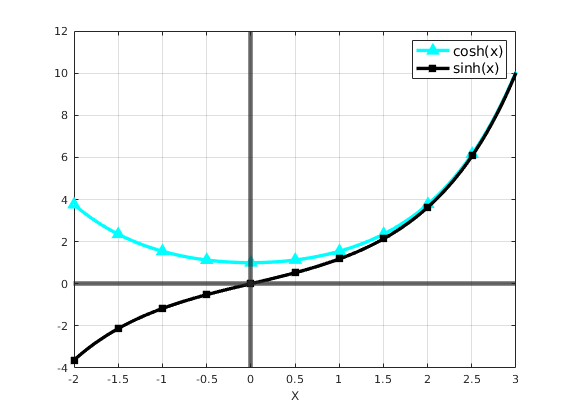
\includegraphics{cosh_and_sinh_plot.png}
\caption{Plot of $\cosh{x}$ and $\sinh{x}$}
\label{fig:cosh-and-sinh-plot}
\end{marginfigure}


For reasons that will become clear later in the course, it is sometimes useful to re-express the solution shown in Equation \ref{eq:sp-case-1-exp} in terms of the functions $\cosh$ and $\sinh$.  These functions are defined as linear combinations of exponentials as shown below and plotted in Figure \ref{fig:cosh-and-sinh-plot}
\begin{align*}
\cosh{x} &= \frac{e^{x} + e^{-x}}{2} \\
\sinh{x} &= \frac{e^{x} - e^{-x}}{2}
\end{align*}



\item \textbf{Real Repeated Roots}
In this case $m_1 = m_2$.\marginnote{i.e. from the quadratic equation, $b^2-4ac = 0$}  One solution is:
\begin{equation}
u_1(x) = e^{m_1x}
\end{equation}

The other solution so derived is, of course, the same and thus we do not have two linearly independent solutions as required to form a fundamental set of solutions for a 2\textsuperscript{nd}-order linear homogeneous equation.  

\newthought{It can be shown} that a second linearly independent solution can be formed by multiplying by the independent variable:\marginnote{This is done using a technique referred to as \emph{reduction of order}.  We will not take the time to cover it in this class (or in this book) but is concisely described in section 3.2 of Zill.  At a minimum you might at least confirm for yourself that a) $xu_1(x)$ is a solution to the equation; and b) use the Wronskian to confirm that it is linearly independent from $u_1(x)$.}
\begin{equation*}
u_2(x) = x u_1(x) = xe^{mx}
\end{equation*}
and thus the general solution for this case is:
\begin{equation}
u(x) = c_1e^{mx}+c_2xe^{mx}
\label{eq:rep-real-roots}
\end{equation}

\item \textbf{Conjugate Complex Roots}
In this case the discriminant, $b^2-4ac$, is negative so its square root is imaginary.  This results in $m_1$ and $m_2$ being complex conjugates which we will express as: $m_1 = \alpha + i\beta$ and $m_2 = \alpha - i\beta$.

The general solution is:
\begin{align*}
u(x) &= c_1e^{(\alpha + i\beta)x}+c_2e^{(\alpha - i\beta)x} \\
&=e^{\alpha x}\left(c_1e^{i\beta x} + c_2e^{-i\beta x} \right) 
\end{align*}

The complex exponentials in the last equation can be re-expressed using the Euler Formula:\index{Formula, Euler}
\begin{align*}
e^{i\beta x} &= \cos{\beta x} + i \sin{\beta x} \\
e^{-i\beta x} &= \cos{\beta x} - i \sin{\beta x}
\end{align*}
which is slighly more convenient insofar as the solutions are no longer expressed as complex exponentials but also by breaking each solution down into their real and complex parts. It can be shown that both the real and imaginary parts of the solution must satisfy the differential equation \emph{independently}.  This fact allows us to re-express the solution in a more simple form that does not involve complex numbers:
\begin{equation}
u(x) = e^{\alpha x}\left(c_1 \cos{\beta x} + c_2 \sin{\beta x} \right)
\label{eq:cmplx-conj-roots}
\end{equation}

\newthought{Another important} special case is when the solution is \emph{pure imaginary} (i.e. $\alpha = 0$) so the solution is:
\begin{equation}
u(x) = c_1 \cos{\beta x} + c_2 \sin{\beta x}
\end{equation}
These solutions arise when the governing equation is of the shown in Equation \ref{eq:special-case-2}:
\begin{equation}
u^{\prime \prime} + k^2 u = 0
\label{eq:special-case-2}
\end{equation}
The roots $m_{1,2} = \pm ik$ and the general solution is:
\begin{equation}
u(x)=c_1 \cos{kx} + c_2 \sin{kx}
\end{equation}
This equation will be revisited throughout the course as it repeatedly comes up in applications.
\end{enumerate}

\section{Three Examples}
The cases described above will be illustrated with three examples:

\vspace{0.5cm}
\noindent\textbf{Example \#1:}
Find the general solution to $2u^{\prime \prime}-5u^{\prime}-3u = 0$. Inserting $u = e^{mx}$ into the equation gives us the auxiliary equation:
\begin{equation*}
2m^2 - 5m - 3 = (2m+1)(m-3)
\end{equation*}
with roots: $m_1 = -\frac{1}{2}$ and $m_2 = 3$.  These are real, distinct roots so the general solution is:
\begin{equation*}
u(x) = c_1e^{-x/2}+c_2e^{3x}
\end{equation*}

\vspace{0.5cm}

\noindent\textbf{Example \#2:}
Find the general solution to $u^{\prime \prime}-10u^{\prime}+25u = 0$.
The auxiliary equation is:
\begin{equation*}
m^2-10m+25 = (m-5)(m-5)
\end{equation*}
with (repeated) roots: $m_1 = 5$ and $m_2 = 5$.  These are real, repated roots so the general solution is:
\begin{equation*}
u(x) = c_1e^{5x} + c_2xe^{5x}
\end{equation*}

\vspace{0.5cm}

\noindent\textbf{Example \#3:}
Find the general solution to $4u^{\prime \prime}+4u^{\prime} + 17u = 0, \ \ u(0)=-1, \ u^{\prime}(0)=2$.

This is an initial value problem\marginnote{We can see that it must be an \emph{initial} value problem because the conditions are both given at the same location, $x_0=0$.} with continuous (and constant) coefficients.  We know from Theorem \ref{thm:IVP-exist-and-unique} that a unique solution exists.  We will first find the general solution, then apply the initial conditions to resolve the unknown coefficients to reveal the solution.

The auxiliary equation is:
\begin{align*}
4m^2+4m+17 &= 0 \\
\text{using the quadratic equation, gives us:} \\
\frac{-4 \pm \sqrt{16 - 4(4)(17)}}{2(4)} &= -\frac{1}{2} \pm \frac{\sqrt{-256}}{8}\\
&= -\frac{1}{2} \pm \frac{-16}{8} \\
&= -\frac{1}{2} \pm 2i
\end{align*}
This gives us complex conjugate roots and the general solution is:
\begin{equation*}
u(x) = e^{-x/2}\left(c_1 \cos{2x} + c_2 \sin{2x} \right)
\end{equation*}
Applying the initial condition $u(0)=-1$ gives us:
\begin{align*}
u(0) &= e^{0}\left(c_1 \cos{0} + c_2 \sin{0} \right) \\
&= 1(c_1(1)+c_2(0)) \\
&= c_1 = -1
\end{align*}
To apply the second initial condition we need to use the chain-rule and product rule to differentiate the general solution.  This gives us:
\begin{multline*}
u^{\prime}(x) = -\frac{1}{2}e^{-x/2}c_1\cos{2x}-2e^{-x/2}c_1\sin{2x} + \\
-\frac{1}{2}e^{-x/2}c_2\sin{2x}+2e^{-x/2}c_2\cos{2x}
\end{multline*}
Evaluating $u^{\prime}(0)$ and substituting $c_1 = -1$ gives us:
\begin{align*}
u^{\prime}(0) &= -\frac{1}{2}(1)(-1)(1) + (1)(2)c_2(1) \\
&= \frac{1}{2}+2c_2 = 2 \\
  \Rightarrow 2c_2 &= \frac{3}{2} \\
 c_2 &= \frac{3}{4}
\end{align*}
Both constants are now known and the unique solution is:
\begin{equation*}
u(x) = e^{-x/2}\left(-\cos{2x}+\frac{3}{4}\sin{2x} \right)
\end{equation*}

\chapter{Lecture 5 - Non-homogeneous Linear Equations with Constant Coefficients}
\label{ch:lec5}
\section{Objectives}
The objectives of this lecture are:
\begin{itemize}
\item Describe the Method of Undetermined Coefficients for solving non-homogeneous linear equations with constant coefficients.
\item Carry out some examples to illustrate the methods.
\end{itemize}
In this lecture we will review \emph{a} method for finding solutions to non-homogeneous linear equations with constant coefficients.\marginnote{To be perfectly honest, we spend very little time in this class dealing with non-homogeneous equations of any kind; many of those types of equations are beyond our ability to solve analytically so we turn to numerical methods instead. Nonetheless there is value in reminding ourselves how to construct solutions for those cases where we can.}
\section{Background}
\newthought{Consider the equation} 
\begin{equation}
a_nu^{(n)} + a_{n-1}u^{(n-1)}+\cdots+a_1u^{\prime}+a_0u = g(x)
\label{eq:cc_nonhomo}
\end{equation}
where
\begin{itemize}
\item the coefficients $a_i, \ i\in [1,2,\dots,n]$ are constants; and
\item the function $g(x)$ is a constant, a polynomial function, exponential function, sine or cosine, or finite sums or products of these functions.
\end{itemize}
The general solution, $u(x)$, can be constructed as $u_c(x)+u_p(x)$ where
\begin{itemize}
\item $u_c(x)$ is the complementary solution which, as you should recall, is the general solution to the associated homogeneous problem. [i.e. Equation \ref{eq:cc_nonhomo} with $g(x)=0$]; and
\item $u_p(x)$ is (any) particular solution---that is, a not-necessarily-unique function that satisfies Equation \ref{eq:cc_nonhomo}.
\end{itemize}
We spent the last lecture describing, effectively, how to find $u_c(x)$; the question this lecture will hope to answer is: ``How do I find $u_p(x)$?''  
\section{Method of Undetermined Coefficients}\index{Undetermined Coefficients}
One method for finding $u_p(x)$ is called the Method of Undetermined Coefficients.\sidenote{Some people lovingly refer to this technique as "The Method of Guessing."}

\newthought{There are three} parts to this technique

\begin{enumerate}
\item \textbf{Basic Rule:} based on the terms in $g(x)$, select the appropriate form for $u_p(x)$ using Table \ref{tab:method-of-guessing-table}.

\begin{table}[h]
\begin{center}
\begin{tabular}{|c|l|}
%\toprule
\hline
Term in $g(x)$ & Choice for $u_p(x)$ \\\hline%\midrule

$ke^{\gamma x}$ & $Ae^{\gamma x}$ \\\hline
$kx^{n}, \ (n=0,1,\dots)$ & $K_nx^n+K_{n-1}x^{n-1}+\cdots +K_1x+K_0$\\\hline
$k \cos{\omega x}$ & \multirow{2}{*}{$\Big\} \ K\cos{\omega x} + M\sin{\omega x}$}\\\cline{1-1}
$k \sin{\omega x}$ &                 \\\hline
$ke^{\alpha x}\cos{\omega x}$   & \multirow{2}{*}{$\Big\} \ e^{\alpha x}\left(K\cos{\omega x} + M\sin{\omega x}\right)$}\\\cline{1-1} 
$ke^{\alpha x}\sin{\omega x}$ &      \\\hline
%\bottomrule
\end{tabular}
\end{center}
\caption{Forms of $u_p(x)$ for given terms in $g(x)$}
\label{tab:method-of-guessing-table}
\end{table}

\item \textbf{Modification rule:} if $u_p(x)$ obtained by the \textbf{Basic Rule} happens to be a solution to the associated homogeneous equation, multiply $u_p(x)$ from the table by $x$ (or $x^2$ if needed).

\item \textbf{Sum rule:} if $g(x)$ is a linear combination of terms from the left-hand column, construct $u_p(x)$ from a linear combination of the corresponding entries in the right-hand column.
\end{enumerate}
For the remainder of this lecture, we will practice applying these rules to some example problems.

\vspace{0.5cm}

\noindent{\textbf{Example:}} solve $u^{\prime \prime}+4u^{\prime}-2u = 2x^2 - 3x + 6$

\vspace{0.25cm}
\noindent{\textbf{Step \#1:}} find the general solution to the associated homogeneous equation.

\vspace{0.25cm}

\noindent The auxiliary equation is: $m^2 + 4m-2=0$; using the quadratic equation gives us:\marginnote{Here you are expected to examine the associated homogeneous problem as $u^{\prime \prime}+4u^{\prime}-2u =0$, identify it as constant coefficient and linear, and solve by assuming $u=e^{mx}$ and thus deriving the auxiliary equation shown without further prompting.} 
\begin{align*}
m &= \frac{-4 \pm \sqrt{16 - (4)(1)(-2)}}{2(1)} \\
&= -2 \pm \frac{\sqrt{24}}{2} \\
&= -2 \pm \sqrt{6}
\end{align*}
so $u_c(x) = c_1e^{(-2+\sqrt{6})x}+c_2e^{(-2-\sqrt{6})x}$

\vspace{0.25cm}
\noindent{\textbf{Step \#2:}} Apply the method of undetermined coefficients to construct a candidate $u_p(x)$.

\vspace{0.25cm}

\noindent Since $g(x)$ is a second-order polynomial, the table tells us $u_p(x)$ is in the general form of a second-order polynomial.
$$u_p(x) = K_2x^2+K_1x+K_0$$
We plug this into the governing equation and this gives us:
\begin{equation*}
2K_2 + 4(2K_2x+K_1) - 2(K_2x^2+K_1x+K_0) = 2x^2-3x+6
\end{equation*}
Now we need to equate the coefficient for each power of $x$:

\begin{table*}[h!]
\begin{tabular}{l r l}
$x^2$:&$-2K_2 $&$= 2$ \\
$x$:& $8K_2 - 2K_1$ &$= -3$ \\
$1$:&$2K_2+4K_1-2K_0$ &$= 6$
\end{tabular}
\end{table*}
Luckily for us, this system of equations is structured such that it can easily be solved.  We see by inspection that $K_2 = 2/-2 = -1$; this can be plugged into the second equation to find $K_1 = -5/2$ and then we can solve the last equation to find that $K_0 = -9$.\marginnote[-4.0cm]{In general you cannot expect this to go so nicely.  What you \emph{can} hope for is that the, in this case, three equations you derive will have a unique solution.  We could re-write the system in the form of a matrix-vector equation:
\begin{equation*}
\begin{bmatrix}
0 & 0 & -2 \\
0 & -2 & 8 \\
-2 & 4 & 2
\end{bmatrix}
\begin{bmatrix}
K_0 \\
K_1 \\
K_2
\end{bmatrix}
= 
\begin{bmatrix}
2 \\
-3 \\
6
\end{bmatrix}
\end{equation*}
If the solution of such a matrix cannot be done by inspection and simple algebra as it was in this case, we could use tools like MATLAB to solve the linear system of equations.  This topic and much more is covered in the numerical methods portion of this text.}

Thus the particular solution is:
\begin{equation*}
u_p(x) = -x^2-\frac{5}{2}x -9
\end{equation*}

\vspace{0.25cm}
\noindent\textbf{Step \#3:} Construct the general solution: $u(x) = u_c(x)+u_p(x)$.

\vspace{0.25cm}

\noindent We now have both the complementary solution and a particular solution; we form the general solution to the equation by adding them together.
\begin{align*}
u(x) &= u_c(x)+u_p(x) \\
&= c_1e^{(-2+\sqrt{6})x}+c_2e^{(-2-\sqrt{6})x}-x^2-\frac{5}{2}x -9
\end{align*}\marginnote[-1.5cm]{Why, again, do we need the constants $c_1$ and $c_2$?

\vspace{0.5cm}

\noindent\textbf{Answer: }Because we have not yet applied initial/boundary conditions.  If those conditions are provided---two conditions for a 2\textsuperscript{nd}-order problem---then we can resolve the constants.
}

\vspace{0.5cm}

\noindent\textbf{Example:} solve $u^{\prime \prime}-5u^{\prime}+4u=8e^x$

\vspace{0.25cm}

\noindent\textbf{Step \#1:} find the general solution to the associated homogeneous problem.

\vspace{0.25cm}

\noindent The auxiliary equation is $m^2-m+4=0$ the left side of which can easily be factored to give $(m-4)(m-1)=0$; the roots of which are $m_1=4$, $m_2=1$.  The complementary solution is:
\begin{equation*}
u_c(x) = c_1e^{4x}+c_2e^{x}
\end{equation*} 

\noindent\textbf{Step \#2:} Apply the method of undetermined coefficients to construct $u_p(x)$.

\vspace{0.25cm}

\noindent Inspecting Table \ref{tab:method-of-guessing-table} we see that $u_p(x)$ should be of the form $Ae^{x}$.  If that function seems vaguely familiar it may be because $e^x$ is part of the complementary solution. 

\vspace{0.25cm}

\noindent\textbf{Pop Quiz:} if you plug $Ae^{x}$ into your governing equation, without doing any calculations, what value should you get?

\vspace{0.25cm}

\noindent\textbf{Answer:} you will get zero!  Why? Because $e^{x}$ is one of the two linearly independent solutions to the associated homogeneous problem. 

\vspace{0.25cm}

\noindent\textbf{What do I do now?}

\vspace{0.25cm}

\noindent\textbf{Answer: } invoke the Modification Rule---this is, after all, the reason why the rule exists---and multiply $u_p$ by $x$.  We now have $u_p(x) = Axe^x$.

\vspace{0.25cm}

\noindent We insert this proposed function for $u_p(x)$ into the equation and we get:
\begin{equation*}
2Ae^x+Axe^x - 5(Ae^x+Axe^x) + 4Axe^x = 8e^x
\end{equation*} 
Combine terms and solve for $A$:
\begin{align*}
2Ae^x-5Ae^x &= 8e^x \\
-3Ae^x &= 8e^x \\
A &= -\frac{8}{3}
\end{align*}
So the particular solution is:
\begin{equation*}
u_p(x) = -\frac{8}{3}xe^x
\end{equation*}

\vspace{0.25cm}
\noindent\textbf{Step \#3:} Construct the general solution: $u(x)=u_c(x)+u_p(x)$.
\marginnote{\textbf{Note:} If any of this seems at all sketchy to you, the good news is that you need not worry if your proposed $u_p(x)$ is any good; you can just plug it into the differential equation and find out!}
\begin{align*}
u(x) &= u_c(x)+u_p(x) \\
&=c_1e^{4x}+c_2e^x - \frac{8}{3}xe^{x}
\end{align*}

\newthought{This last example} illustrates the use of the Sum Rule; it also includes initial condition so the unique solution to the initial value problem can be found.

\vspace{0.25cm}

\noindent\textbf{Example:} solve the initial value problem: $u^{\prime \prime}+u=4x+10\sin{x}$ with initial conditions $u(\pi)=0, \ u^{\prime}(\pi)=2$.

\vspace{0.25cm}

\noindent\textbf{Step \#1:} Find the general solution to the associated homogeneous problem.

\vspace{0.25cm}

\noindent The auxiliary equation is: $m^2+1=0$, therefore $m=\pm i$ and $u_c(x)$ can be found as:
\begin{equation*}
u_c(x) = c_1\cos{x}+c_2\sin{x}
\end{equation*}

\vspace{0.25cm}

\noindent\textbf{Step \#2:} Apply the method of undetermined coefficients to construct $u_p(x)$.

\vspace{0.25cm}

\noindent For this problem, $g(x) = 4x+10\sin{x}$ has two terms, so we will construct $u_p(x)$ using one term at a time; $u_{p_1}(x)$ using $4x$ and $u_{p_2}(x)$ using $10\sin{x}$.\marginnote[-1.0cm]{It's the linearity property of $\mathcal{L} = \frac{d^2}{dx}+1$ that makes this possible. If $\mathcal{L}(u_{p_1})=4x$ and $\mathcal{L}(u_{p_2})=10\sin{x}$ then $\mathcal{L}(u_{p_1}+u_{p_2})=4x+10\sin{x}$.}  

\vspace{0.25cm}

\noindent\textbf{Step \#2.a:} Find $u_{p_1}(x)$.

\vspace{0.25cm}

\noindent From Table \ref{tab:method-of-guessing-table}, for $g(x)=4x$, we should select $u_{p_1} = K_1x+K_0$.  Inserting this into the differential equation gives us: $K_1x + K_0 = 4x$.  By inspection we can see that $K_0 = 0$ and $K_1 = 4$ so $u_{p_1}(x) = 4x$.  

\vspace{0.25cm}

\noindent\textbf{Step \#2.b: } Find $u_{p_2}(x)$.

\vspace{0.25cm}

\noindent From Table \ref{tab:method-of-guessing-table}, for $g(x)=10\sin{x}$, we should select $u_{p_2} =  K\cos{x}+M\sin{x}$. Now that we have done this a couple of times we should be on the alert for portions of the complementary solution cropping up in our guesses for $u_p(x)$ so we immediately see that we must multiply $u_{p_2}$ by $x$.  If we do this and insert $Kx\cos{x}+Mx\sin{x}$ into the differential equation we get:
\begin{multline*}
\left(-2K-Mx\right)\sin{x}+\left(2M-Kx\right)\cos{x} + \dots \\ Kx\cos{x}+Mx\sin{x} = 10\sin{x}
\end{multline*}

\vspace{0.25cm}

\noindent Matching coefficients for $\sin{x}$ and $\cos{x}$ on both sides of the above equation leads us to conclude that $M=0$ and $-2K = 10$.  Therefore $K = -5$ and $u_{p_2}(x)=-5x\cos{x}$.\marginnote{Again, there is no harm in testing your proposed $u_{p_2}(x)$ to see if it does indeed produce the expected result.}

\vspace{0.25cm}

\noindent\textbf{Step \#3:} Construct the general solution: $u(x)=u_c(x)+u_p(x)$.

\begin{align*}
u(x) &= u_c(x) + u_p(x) \\ 
&= u_c(x) + u_{p_1}(x)+u_{p_2}(x) \\
&= c_1\cos{x}+c_2\sin{x}+4x-5x\cos{x}
\end{align*}

\newthought{All that remains} is to apply the initial conditions.  

\begin{align*}
u(\pi) &= c_1(-1)+c_2(0)+4\pi -5(\pi)(-1) \\
&=-c_1+9\pi = 0 \\
\Rightarrow &= c_1 = 9\pi
\end{align*}

\vspace{0.25cm}

\noindent Applying the initial condition $u^{\prime}=2$:
\begin{equation*}
u^{\prime}(\pi)=-9\pi(0)+c_2(-1)+4-5(-1)+5\pi(0)=2
\end{equation*}

\vspace{0.25cm}

\noindent Solving for $c_2$ gives us: $c_2 = 7$; folding this into the general solution:

\begin{equation*}
u(x) = 9\pi \cos{x}+7\sin{x}+4x-5x\cos{x}
\end{equation*}

\chapter{Assignment \#2}
\label{ch:ass2}
\begin{fullwidth}
The given family of functions is the general solution of the differential equation on the indicated interval.  Find a member of the family (i.e. find the values for the constants $c_1$ and $c_2$) that is a solution of the initial-value problem.

\begin{enumerate}[series=outerlist]
\item $u=c_1e^{x}+c_2e^{-x}; \ \ u^{\prime \prime}-u=0, \ u(0)=0, \ u^{\prime}(0)=1$

\vspace{1.0cm}

\item $u=c_1x + c_2x \ln{x}, \ \ (0,\infty), \ x^2u^{\prime \prime}-xu^{\prime}=0, \ u(1)=3, \ u^{\prime}(1)=-1$

\vspace{1.0cm}
\end{enumerate}

\noindent The given two-parameter family is a solution of the indicated differential equation on the interval $(-\infty,\infty)$.  Determine if a member of the family can be found that satisfies the boundary conditions.

\begin{enumerate}[resume=outerlist]
\item $u=c_1e^{x}\cos{x} + c_2e^{x}\sin{x}; \ \ u^{\prime \prime}-2u^{\prime}+3u=0$

\begin{enumerate}[series=innerlist]
\item $u(0)=1, \ u^{\prime}(\pi)=0$

\item $u(0)=1, \ u(\pi)=-1$

\item $u(0)=1, \ u(\pi/2)=1$

\item $u(0)=0, \ u(\pi)=0$
\end{enumerate}

\vspace{1.0cm}
\end{enumerate}
Determine if the given set of functions is linearly dependent or linearly independent on the interval $(-\infty,\infty)$.


\begin{enumerate}[resume=outerlist]
\item $f_1(x)=x, \ \ f_2(x)=x^2, \ \ f_3(x)=4x-3x^2$

\vspace{1.0cm}

\item $f_1(x)=1+x, \ \ f_2(x)=x, \ \ f_3(x)=x^2$
\vspace{1.0cm}
\end{enumerate}


\noindent Verify that the given two-parameter family of functions is the general solution of the non-homogeneous differential equation on the indicated interval.

\begin{enumerate}[resume]
\item $u^{\prime \prime}-7u^{\prime}+10u=24e^{x}, \ \ u=c_1e^{2x}+c_2e^{5x}+6e^{x}, \ \left(-\infty,\infty\right)$

\vspace{1.0cm} 

\end{enumerate}

\noindent Find the general solution to the given second-order differential equation.

\begin{enumerate}[resume]
\item $4u^{\prime \prime}+u^{\prime} = 0$

\vspace{1.0cm}

\item $u^{\prime \prime}-u^{\prime}-6u=0$

\vspace{1.0cm}

\item $u^{\prime \prime}+8u^{\prime}+16u=0$

\vspace{1.0cm}

\item $u^{\prime \prime}+9u=0$

\vspace{1.0cm}
\end{enumerate}


\noindent Solve the given initial-value problem.

\begin{enumerate}[resume]
\item $u^{\prime \prime}+16u=0, \ \ u(0)=2, \ u^{\prime}(0)=-2$

\vspace{1.0cm}

\item $u^{\prime \prime}-4u^{\prime}-5u=0, \ \ u(1)=0, \ u{\prime}(1)=2$

\vspace{1.0cm}

\item $u^{\prime \prime}+u =0, \ \ u^{\prime}(0)=0, \ u^{\prime}(\pi/2)=0$

\vspace{1.0cm}

\end{enumerate}

\noindent Solve the given differential equation using the Method of Undetermined Coefficients.

\begin{enumerate}[resume]
\item $u^{\prime \prime}-10u^{\prime}+25u=30x+3$

\vspace{1.0cm}

\item $u^{\prime \prime}+3u=-48x^2e^{3x}$

\vspace{1.0cm}
\end{enumerate}

\noindent Solve the given initial-value problem.

\begin{enumerate}[resume]
\item $5u^{\prime \prime} + u^{\prime} - 6x, \ \ u(0)=0, \ u^{\prime}(0)=-10$

\vspace{1.0cm}

\end{enumerate}

\noindent Solve the given boundary-value problem.

\begin{enumerate}[resume]
\item $u^{\prime \prime}+u=x^2+1, \ \ u(0)=5, \ u(1)=0$

\vspace{1.0cm}

\end{enumerate}

\noindent Solve the given initial-value problem in which the input function $g(x)$ is discontinuous. (\textbf{Hint:} Solve the problem on two intervals and then find a solution so that $u$ and $u^{\prime}$ are continuous at the boundary of the interval.)

\begin{enumerate}[resume]
\item $u^{\prime \prime}+4u=g(x), \ \ u(0)=1, \ u^{\prime}(0)=2$
\begin{equation*}
g(x) = 
\begin{cases}
\sin{x} & 0 \le x \le \pi/2 \\
0 & x > \pi/2
\end{cases}
\hspace{12cm}
\end{equation*}

\end{enumerate}


\end{fullwidth}

\chapter{Lecture 6 - Newton's Method for Systems of Non-Linear Equations}
\label{ch:lec6n}
\section{Objectives}
The objectives of this lecture are to:
\begin{itemize}
\item Describe Newton's method for finding roots to systems of non-linear equations.
\item Do an example problem.
\item Describe MATLAB functions for solving a system of non-linear equations.
\end{itemize}
\setcounter{lstannotation}{0}

\section{Newton's Method for Systems of Non-Linear Equations}

In Lecture 4 we derived Newton's method for finding the root to a single non-linear equation.  The basic iteration procedure was to update our estimate of the root according to the equation:
\begin{equation*}
x_{i+1} = x_i - \frac{f(x_i)}{f^{\prime}(x_i)}
\end{equation*}
The idea on which this was derived was to project a line tangent to $f(x_i)$ to the $x$-axis. 

\index{Taylor series expansion}
\newthought{An alternative way} to derive this update relation is based on the Taylor series expansion.  In a Taylor series expansion, given a function evaluated at some point, $f(x_1)$, we estimate the value of the function at some \emph{other} point, $x_2$, using the equation below:

\begin{align*}
f(x_2) &= f(x_1) +  \frac{f^{\prime}(x_1)}{1!}(x_2 - x_1) +  \frac{f^{\prime \prime}(x_1)}{2!}(x_2 - x_1)^2 + \cdots \\
&= \sum\limits_{n=0}^{\infty} \frac{f^{(n)}(x_1)}{n!}(x_2 - x_1)^n
\end{align*}
If we ignore terms proportional to $f^{\prime \prime}(x_1)$ and higher, and if we suppose that $x_2$ is a root, we get:
\begin{align*}
f(x_2) = 0 &= f(x_1) + f^{\prime}(x_1)(x_2 - x_1) \\
x_2 - x_1 &= \frac{-f(x_1)}{f^{\prime}(x_1)} \\
\Rightarrow x_2 &= x_1 - \frac{f(x_1)}{f^{\prime}(x_1)} 
\end{align*}
which is the same as what we started with.

\newthought{We would now} like to generalize Newton's method to find roots for a \emph{system} of two or more equations.  We will use the formulation based on the Taylor series expansion to do this.  

Consider the case of 2 non-linear functions of 2 variables:
\begin{equation*}
f_1(x,y) = 0 , \ \ f_2(x,y) = 0
\end{equation*}
If $x_2$ and $y_2$ are the true (unknown) solution to the equations, and $x_1$ and $y_1$ are points sufficiently close to the solution then:
\begin{align*}
f_1(x_2,y_2) &= 0 = f_1(x_1,y_1) + (x_2 - x_1) \frac{\partial f_1}{\partial x}\Bigr|_{x_1,y_1} + (y_2 - y_1) \frac{\partial f_1}{\partial y}\Bigr|_{x_1,y_1}  \\
f_2(x_2,y_2) &= 0 = f_2(x_1,y_1) + \underbrace{(x_2 - x_1)}_{\Delta x} \frac{\partial f_2}{\partial x}\Bigr|_{x_1,y_1} + \underbrace{(y_2 - y_1)}_{\Delta y} \frac{\partial f_2}{\partial y}\Bigr|_{x_1,y_1} \\
\end{align*}
where higher order terms are neglected.  This set of linear equations can be expressed in a matrix-vector format as shown in Equation \ref{eq:lec6n-matvec}.

\index{Jacobian}
\begin{equation}
\bracketMatrixstack{
\frac{\partial f_1}{\partial x}\Bigr|_{x_1,y_1} & \frac{\partial f_1}{\partial y}\Bigr|_{x_1,y_1} \\
\frac{\partial f_2}{\partial x}\Bigr|_{x_1,y_1} & \frac{\partial f_2}{\partial y}\Bigr|_{x_1,y_1}
}
\bracketVectorstack{
\Delta x \\
\Delta y
}
=
\bracketVectorstack{
-f_1(x_1,y_1) \\
-f_2(x_1,y_1)
}
\label{eq:lec6n-matvec}
\end{equation}
The unknown quantities are $\Delta x$ and $\Delta y$.  The matrix in Equation \ref{eq:lec6n-matvec} is referred to as the \emph{Jacobian}. We can solve this linear system of equations\sidenote{Actually we have not covered how to do that yet in this class.  Students can probably solve this $2 \times 2$ system of equations based on their experience in high school math, but we will thoroughly study methods for solving linear systems of equations in the next section of the text.} to find $\Delta x$ and $\Delta y$ and thus get $x_2$ and $y_2$ from Equation \ref{eq:lec6n-xy-update}.
\begin{equation}
x_2 = x_1 + \Delta x, \ \ \ y_2 = y_1 + \Delta y
\label{eq:lec6n-xy-update}
\end{equation}

\vspace{4.0cm}

\newthought{In summary,} Newton's method for solving a system of non-linear equations is made up of the following steps:
\begin{enumerate}
\item Start with an initial guess, $x_1$, $y_1$.
\item Form and solve the linear system of equations given in Equation \ref{eq:lec6n-matvec} to obtain $\Delta x$ and $\Delta y$.
\item compute $x_{i+1}$ and $y_{i+1}$ from: $x_{i+1} = x_{i} + \Delta x, $ and $ y_{i+1} = y_{i} + \Delta y$.
\item Repeat steps \#2 and \#3 until $\Delta x$ and $\Delta y$ are within some specified error tolerance.\sidenote{We will use a relative error tolerance that will be illustrated in the example code.}
\end{enumerate}

\vspace{0.25cm}

\noindent\textbf{Example:} The equations of the catenary curve and the ellipse, which are shown in Figure \ref{fig:lec6n-ex1}, are given by:
\begin{marginfigure}
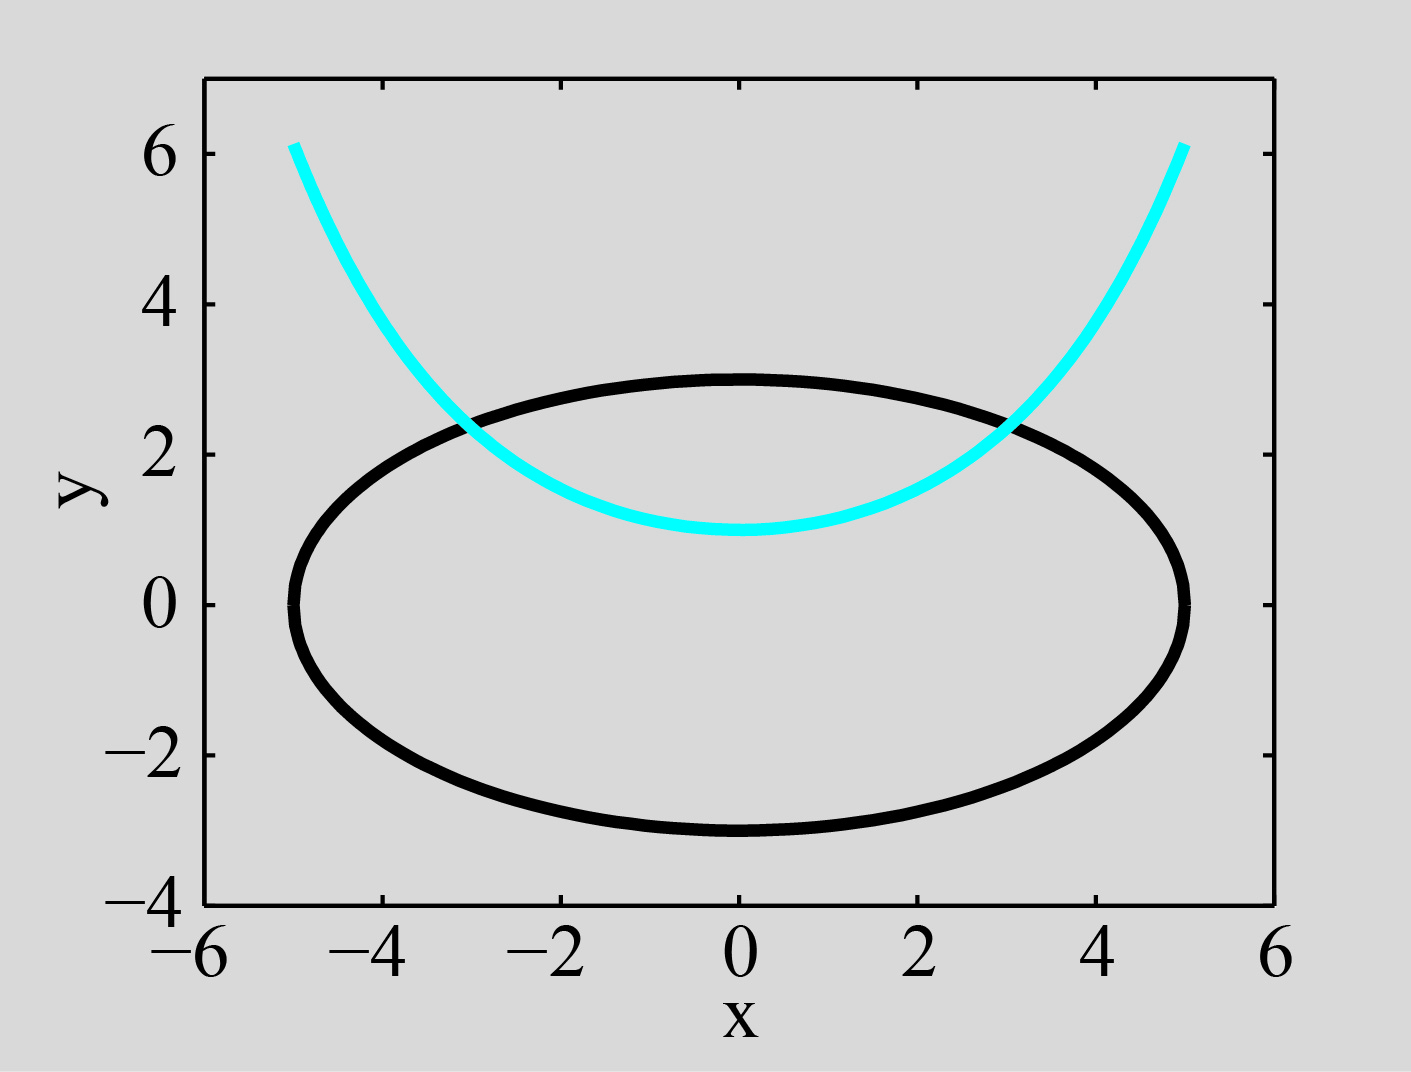
\includegraphics{Chapter3Example3_5.jpg}
\caption{Example system of non-linear equations.}
\label{fig:lec6n-ex1}
\end{marginfigure}
\begin{align*}
f_1(x,y) &= y-\frac{1}{2}\left(e^{\sfrac{x}{2}} + e^{-\sfrac{x}{2}}\right) \\
f_2(x,y) &= 9x^2 + 25y^2 - 225
\end{align*}
Use Newton's method to determine the point of intersection of the curves that resides in the first quadrant of the coordinate system.

\vspace{0.15cm}

\noindent The Jacobian for this system of equations is given by:
\begin{equation*}
\bracketMatrixstack{
-\frac{1}{4}\left(e^{\sfrac{x}{2}} + e^{-\sfrac{x}{2}}\right) & 1 \\
18x & 50y 
}
\end{equation*}

\vspace{0.15cm}

\noindent We begin by clearing out the workspace and defining the given functions and the Jacobian:
\begin{lstlisting}[style=myMatlab, name=lec6n-ex1]
clear
clc
close 'all'

F1 = @(x,y) y - 0.5*(exp(x./2) + exp(-x./2));
F2 = @(x,y) 9*x.^2 + 25*y.^2 - 225;

dF1x = @(x,y) -0.25*(exp(x./2) - exp(-x./2));
dF1y = @(x,y) 1;

dF2x = @(x,y) 18*x;
dF2y = @(x,y) 50*y;

Jac = @(x,y) [dF1x(x,y) dF1y(x,y); dF2x(x,y) dF2y(x,y)];
\end{lstlisting}

\vspace{0.15cm}

\noindent Next we will define $x_1$ and $y_1$ and specify our stopping criteria.
\begin{lstlisting}[style=myMatlab,name=lec6n-ex1]
xi = 2.5; yi = 2; 
Err = 1e-10; imax = 10;
\end{lstlisting}
Note that we do not plan on making many iterations.  If Newton's method works, it will very quickly converge.

\vspace{0.25cm}

\noindent Now we implement Newton's method:\marginnote[1.0cm]{
\ref{lst:ann6n-1} We use MATLAB's built-in ``backslash'' operator to solve the linear system of equations.  This will be discussed in Section VIII of this text.

\vspace{0.3cm}


\ref{lst:ann6n-2} Here we compare $\sfrac{\Delta x}{x}$ and $\sfrac{\Delta y}{y}$ for our relative error tolerance.  We are really not computing the error, we are computing how small our updates are to $x$ and $y$.

\vspace{0.5cm}

\ref{lst:ann6n-3} The operator \lstinline[style=myMatlab]{&&} is the logical \emph{and} operator.

}
\begin{lstlisting}[style=myMatlab,name=lec6n-ex1]
for i = 1:imax
   J = Jac(xi,yi);
   F = -[F1(xi,yi); F2(xi,yi)];
   dp = J\F;   /*!\annotation{lst:ann6n-1}!*/
   xip = xi + dp(1);
   yip = yi + dp(2);
   Err_x = abs((xip - xi)/xi);  /*!\annotation{lst:ann6n-2}!*/
   Err_y = abs((yip - yi)/yi);
   
   fprintf('i = %i  x = %-7.4f  y = %-7.4f  Error in x = %-7.4g Error in y = %-7.4g \n',...
       i,xip,yip,Err_x,Err_y);
   
   if (Err_x < Err) && (Err_y < Err)  /*!\annotation{lst:ann6n-3}!*/
       break
   else
       xi = xip; yi = yip;
   end
    
end
\end{lstlisting}
This script converges to the solution $x = 3.0311553917$ and $y=2.38586565356$ in 5 iterations.

\section{Implementation with FSOLVE}
The primary MATLAB built-in function you should use for solving a system of non-linear equations is \lstinline[style=myMatlab]{fsolve}.  The basic syntax for using \lstinline[style=myMatlab]{fsolve} is:
\begin{center}
\begin{tabular}{c}
\begin{lstlisting}[style=myMatlab, frame=none, numbers=none, basicstyle=\small]
x = fsolve(fun,x0);
\end{lstlisting}
\end{tabular}
\end{center}
A more complete syntax that provides additional output information and an interface for passing options to the algorithm is:
\begin{center}
\begin{tabular}{c}
\begin{lstlisting}[style=myMatlab, frame=none, numbers=none, basicstyle=\small]
[x, fval, exitflag, output, jacobian] = ...
     fsolve(fun,x0,options);
\end{lstlisting}
\end{tabular}
\end{center}
The values of \lstinline[style=myMatlab]{x} and \lstinline[style=myMatlab]{fval} are similar to what one obtains when using \lstinline[style=myMatlab]{fzero} except, of course they are now both vectors.  Values for \lstinline[style=myMatlab]{exitflag} and \lstinline[style=myMatlab]{output} are different---interested readers should consult the MATLAB documentation---but \lstinline[style=myMatlab]{exitflag=1} still means success.  As with \lstinline[style=myMatlab]{fzero}, a function is used to construct an appropriate \lstinline[style=myMatlab]{options} structure; when using \lstinline[style=myMatlab]{fsolve} you should use the \lstinline[style=myMatlab]{optimoptions} function for this purpose. An example usage of \lstinline[style=myMatlab]{optimoptions} is included in the MATLAB listing below.

\vspace{3.0cm}

\marginnote[4.0cm]{

\ref{lst:ann6n-1} Here we use a \lstinline[style=myMatlab]{switch...case} structure to select between sets of options for purposes of demonstration. The options specified in \lstinline[style=myMatlab]{option_set=1} amount to telling \lstinline[style=myMatlab]{fsolve()} to quietly solve the problem with no output to the command window.  The options specified in \lstinline[style=myMatlab]{option_set=2} specify detailed output on each iteration and provides non-default values for the \lstinline[style=myMatlab]{'MaxIterations'} and \lstinline[style=myMatlab]{'StepTolerance'} parameters.  Consult the MATLAB documentation on \lstinline[style=myMatlab]{fsolve} for more details.

\vspace{3.5cm} 

\ref{lst:ann6n-2} The first argument to \lstinline[style=myMatlab]{fsolve} has to be a (single) handle to a function.  This local function implements the system of two equations from the example. The first argument to \lstinline[style=myMatlab]{ex3p5} is a vector; one element for each equation in our system of equations.

}
\begin{lstlisting}[name=lec6n-ex2, style=myMatlab]
clear
clc
close 'all'

F = @(x) ex3p5(x);
X0 = [2.5, 2.0];

option_set = 2;
% 1 = no outputs
% 2 = detailed outputs

switch option_set     /*!\annotation{lst:ann6n-1}!*/
    
    case 1
        options = optimoptions('fsolve','Display','none');
        
    case 2
        options = optimoptions('fsolve','Display',...
            'iter-detailed','MaxIterations',1000,...
            'StepTolerance',1e-10);
        
    otherwise % default options
        options = optimoptions('fsolve');
        
end

[x,fval,exitflag,output] = fsolve(F,X0,options);

fprintf('Root found at x = %8.7g, y = %8.7g \n',...
    x(1),x(2));
fprintf('fval = \n'); disp(fval);
fprintf('exitflag = %d \n',exitflag);

%% Local Function
function out = ex3p5(x)   /*!\annotation{lst:ann6n-2}!*/
[m,n] = size(x); % expect scalar or vector input
assert(min(m,n)==1,...
    'Error!  Vector input expected for x! \n');
out = nan(m,n); % construct output

out(1) = x(2) - 0.5*(exp(x(1)./2) + exp(-x(1)./2));
out(2) = 9*x(1).^2 + 25*x(2).^2 - 225;

end
\end{lstlisting}
  



\part{Power Series Methods}
\chapter{Lecture 7 - Reveiw of Power Series}
\label{ch:lec7}
\section{Objectives}
The objectives of this lecture are:
\begin{itemize}
\item Review definitions and basic properties of power series.
\item Illustrate important basic operations on power series
\end{itemize}

\section{Introduction and Review}
The methods that we have discussed so far have largely been a review of differential equations class.  Sadly, even in the handful of lectures that we have had, our methods for solving equations are largely exhausted.  We can solve constant coefficient linear equations, and variable coefficient linear equations \emph{if} they happen to be Cauchy-Euler equations.  We can solve many first-order linear equations but if the equation is nonlinear we are sunk unless they happen to be separable.  This leaves out a lot of interesting equations.  In this sequence of lectures we will discuss how to solve linear equations with variable coefficients (other than Cauchy-Euler equations).  To do this we will need to use power series. 

\newthought{You learned about} power series back in calculus class, but you weren't ready to use them for this imporant application.  Now you are and now this is what we will do.  We will begin this section with some definitions that will be needed as we describe the use power series in the solution of differential equations.

\subsection{Definitions}
\begin{definition}[Sequence]
A \emph{sequence} is a list of numbers (or other mathematical objects, like functions) written in a definite order.

\begin{equation*}
\left\{c_0, c_1, c_2, c_3, \dots , c_n\right\}
\end{equation*}
\end{definition}

\index{limit}
\index{convergence}
\index{divergence}
\begin{definition}[Limit of a Sequence, convergence, divergence]
A sequence has a \emph{limit} $(L)$ if we can make the terms $c_n$ arbitrarily close to $L$ by taking $n$ sufficiently large.  If $\lim_{n\to \infty} c_n$ exists, we say the sequence \emph{converges}; otherwise, we say the sequence \emph{diverges} or is \emph{divergence}.
\end{definition}

There are various mathematical tools available for determining if an infinite sequence converges or diverges without needing to examine every element.

\index{series}
\index{infinite series}
\begin{definition}[Series, infinite series]
A \emph{series} is the sum of a sequence. For example, $S_0 = c_0$; $S_1 = c_0+c_1$; $S_n = c_0+c_1+\cdots+c_n$.  If the sequence is infinite, we call the sum an infinite series.
\end{definition}

\begin{definition}[Series Convergence]
Given a series $\sum\limits_{n=0}^{\infty}s_i=s_1+s_2+\cdots+s_n+\cdots$, let $s_n$ denote its $n$\textsuperscript{th} partial sum.  If the sequence $\left\{s_n \right\}$ is convergent then the series is convergent to the same limit.  Otherwise the series is divergent.\marginnote{We will usually use notation such as $s_n\to \infty$ to indicate that the partial sum is unbounded.}
\end{definition}

\index{power series}
\begin{definition}[Power Series]
A series of the form $\sum\limits_{n=0}^{\infty}c_n(x-a)^n=c_0+c_1(x-a)+\cdots$ is called a Power Series. The constant $a$ is referred to as the ``center'' of the power series.\marginnote{For almost all of the power series we will work with in this class, the series will be centered on $a=0$ and will be denoted $\sum\limits_{n=0}^{\infty} c_nx^n$.}
\end{definition}


\index{convergence, interval of}
\index{convergence, radius of}
\begin{definition}[Interval of Convergence, Radius of Convergence]
The set of all real numbers $x$ for which the series converges.  This interval can also be expressed as a \emph{radius of convergence.} ($R$); the series converges for all $a-R < x < a+R$.
\end{definition}

\subsection{Ratio Test}
We should have at least one test that we can use to decide whether or not a series, at least a power series, converges.  The test we will use is called the \emph{Ratio Test}; so named because it involves the ratio of the $n$\textsuperscript{th} and $(n+1)$\textsuperscript{th} term in a power series.  The Ratio Test is shown in Equation \ref{eq:ratio-test}.

\begin{equation}
\lim_{n \to \infty}\left|\frac{c_{n+1}(x-a)^{(n+1)}}{c_n(x-a)^n} \right| = \left|x-a \right| \lim_{n \to \infty} \left|\frac{c_{n+1}}{c_n} \right| = L
\label{eq:ratio-test}
\end{equation}
The following cases are considered:
\begin{itemize}
\item if $L<1$ then the series converges absolutely.\marginnote{\textbf{Note:} \underline{absolute convergence} means that the series converges irrespective of the signs of each term. (i.e. whether or not all terms are positive, negative, or a mix of both positive and negative.)}
\item if $L = 1$ then the test is inconclusive; some other test must be used; and
\item if $L > 1$ then the series diverges.
\end{itemize}





\chapter{Lecture 8 - Gauss Elimination}
\label{ch:lec8n}
\section{Objectives}
The objectives of this lecture are to:
\begin{itemize}
\item Describe Gauss elimination with pivoting algorithm and provide a rationale for its use.
\item Produce a detailed examination of the MATLAB code to implement the algorithm.
\item Introduce the ``Matrix Market'' as a source for relevant test matrices.
\item Run examples illustrating the benefits of this new algorithm.
\end{itemize}
\setcounter{lstannotation}{0}

\section{Gauss Elimination with Pivoting}

One problem with the basic Gauss elimination algorithm presented in the last lecture is the possibility that the pivot will be zero.  In the event of such a pivot, the algorithm will fail and we need to find a way to prevent it from happening if at all possible.  A problem that may appear to be less serious, but nonetheless worthy of our attention, is the case where the pivot is much smaller than other entries in its row and/or column.  Consider the following linear system:
\begin{equation*}
\bracketMatrixstack{
0.0003 & 12.34 \\
0.4321 & 1 
}
\bracketVectorstack{
x_1 \\
x_2
}
=
\bracketVectorstack{
12.343 \\
5.321
}
\end{equation*}   
For the first step of forward-elimination, the pivot element is: 0.0003 and $m_{21} = \sfrac{0.4321}{0.0003} = 1,440.33$.  When I eliminate the $a_{21}$ entry and update the entry for $a_{22}$ and $b_2$:
\begin{equation*}
A(i,j:n) = A(i,j:n) - m*A(j,j:n)
\end{equation*}
the value of $m$ is very large compared to any entry in $A$, and, for lack of a more precise way of putting it, this aggravates roundoff errors in the result. 

The basic idea is: if the pivot is small or zero, why not just exchange the pivot row with a different row?  In order to avoid un-doing any of the forward elimination steps, the row to be exchanged must be ``below'' the current pivot row.  Also, if we want to execute such an exchange, we need to have some criteria by which to decide which row we want to exchange.  The criteria we will use is this: \emph{select the row corresponding to the element in the pivot column with the largest absolute value.} This is most easily clarified with an example.\marginnote[-1.0cm]{For step \lstinline[style=myMatlab]{i} of forward elimination, \lstinline[style=myMatlab]{A(i,i)} is the pivot.  \lstinline[style=myMatlab]{A(i,i:n)} is the pivot row, and \lstinline[style=myMatlab]{A(i:n,i)} is the pivot column.}

\vspace{0.25cm}

\noindent Consider the linear system of equations below:
\begin{equation*}
\bracketMatrixstack{
4 & -2 & -3 & 6 \\
-6 & 7 & 6.5 & -6 \\
1 & 7.5 & 6.25 & 5.5 \\
-12 & 22 & 15.5 & -1 
}
\bracketVectorstack{
x_1 \\
x_2 \\
x_3 \\ 
x_4 
}
=
\bracketVectorstack{
12 \\
-6.5 \\
16 \\
17
}
\end{equation*}
The pivot column is \lstinline[style=myMatlab]{A(1:4,1)} and the entry with the largest magnitude is, -12, in row 4.  We would, therefore, \emph{swap row 1 and 4}.  The system of equations is now:
\begin{equation*}
\bracketMatrixstack{
-12 & 22 & 15.5 & -1 \\
-6 & 7 & 6.5 & -6 \\
1 & 7.5 & 6.25 & 5.5 \\
4 & -2 & -3 & 6  
}
\bracketVectorstack{
x_1 \\
x_2 \\
x_3 \\ 
x_4 
}
=
\bracketVectorstack{
17 \\
-6.5 \\
16 \\
12
}
\end{equation*}
Notice we also had to switch the entries for \lstinline[style=myMatlab]{b(1)} and \lstinline[style=myMatlab]{b(4)}.  We use this pivot to eliminate all of the entries in the first column below the first row.  The resulting system of equations is shown below:
\begin{equation*}
\bracketMatrixstack{
-12 & 22 & 15.5 & -1 \\
0 & -4.0 & -1.25 & -5.5 \\
0 & 9.333 & 7.542 & 5.417 \\
0 & 5.333 & 2.167 & 5.667  
}
\bracketVectorstack{
x_1 \\
x_2 \\
x_3 \\ 
x_4 
}
=
\bracketVectorstack{
17 \\
-15 \\
17.417 \\
17.667
}
\end{equation*}
The pivot column for the next step of forward elimination is now \lstinline[style=myMatlab]{A(2:4,2)} and the element with the largest magnitude is 9.333 in row 3.  We thus swap row 2 and 3 and eliminate the entries in column 2 below row 2.

\begin{equation*}
\underbrace{
\bracketMatrixstack{
-12 & 22 & 15.5 & -1 \\
0 & 9.333 & 7.542 & 5.417 \\
0 & -4.0 & -1.25 & -5.5 \\
0 & 5.333 & 2.167 & 5.667  
}
\bracketVectorstack{
x_1 \\
x_2 \\
x_3 \\ 
x_4 
}
=
\bracketVectorstack{
17 \\
17.417 \\
-15 \\
17.667
}
}_{
\text{Swapped rows 2 and 3.}
}
\rightarrow
\underbrace{
\bracketMatrixstack{
-12 & 22 & 15.5 & -1 \\
0 & 9.333 & 7.542 & 5.417 \\
0 & 0 & -1.982 & -3.189 \\
0 & 0 & -2.143 & 2.571  
}
\bracketVectorstack{
x_1 \\
x_2 \\
x_3 \\ 
x_4 
}
=
\bracketVectorstack{
17 \\
17.417 \\
-7.536 \\
7.714
}
}_{
\text{Eliminate entries below the pivot.}
}
\end{equation*}
Now we have one more entry to eliminate, but, before we do, we will swap the 3\textsuperscript{rd} and 4\textsuperscript{th} row to obtain the largest magnitude pivot.
\begin{equation*}
\underbrace{
\bracketMatrixstack{
-12 & 22 & 15.5 & -1 \\
0 & 9.333 & 7.542 & 5.417 \\
0 & 0 & -2.143 & 2.571   \\
0 & 0 & -1.982 & -3.189
}
\bracketVectorstack{
x_1 \\
x_2 \\
x_3 \\ 
x_4 
}
=
\bracketVectorstack{
17 \\
17.417 \\
7.714 \\
-7.536
}
}_{
\text{Swap 3\textsuperscript{rd} and 4\textsuperscript{th} row.}
}
\rightarrow
\underbrace{
\bracketMatrixstack{
-12 & 22 & 15.5 & -1 \\
0 & 9.333 & 7.542 & 5.417 \\
0 & 0 & -2.143 & 2.571   \\
0 & 0 & 0 & -0.8
}
\bracketVectorstack{
x_1 \\
x_2 \\
x_3 \\ 
x_4 
}
=
\bracketVectorstack{
17 \\
17.417 \\
7.714 \\
-0.4
}
}_{
\text{Eliminate the }a_{4,3}\text{ entry.}
}
\end{equation*}
At this time, we are ready for the back-substitution phase of the algorithm which is unchanged from regular Gauss elimination and, for a small matrix such as in this example, the answer is essentially the same.

\subsection{MATLAB Implementation}
Since the only difference lies in the pivoting, we will restrict our attention to the forward elimination phase of the algorithm.

\vspace{0.25cm}

\marginnote[-1.5cm]{
\ref{lst:ann8n-1} The built-in function \lstinline[style=myMatlab]{max()} takes a vector and returns the largest element along with its index.  Of course the built-in function \lstinline[style=myMatlab]{abs()} returns a vector in which all of the elements are converted to their absolute value. The first return argument to \lstinline[style=myMatlab]{max()} is the actual maximum value but we actually do not need the value; we just need to know which row it is in, which is provided by the return argument \lstinline[style=myMatlab]{j_piv}.  We need both arguments on the right hand side---\lstinline[style=myMatlab]{[~,j_piv]}---but since we never use the first one, instead of storing the result in a variable, we replace the variable with a tilde \lstinline[style=myMatlab]{(~)}.  If we assigned the first argument to a variable but then never used it, MATLAB's code analyzer would issue a warning.  This usage avoids such a warning.   

\vspace{0.15cm} 

\ref{lst:ann8n-2} Since we only used a portion of the column of \lstinline[style=myMatlab]{A} in our call to \lstinline[style=myMatlab]{max}, we need to adjust the value of \lstinline[style=myMatlab]{j_piv} to reflect the true row index of the maximum value in the pivot column.

\vspace{0.15cm}

\ref{lst:ann8n-3} This---save, over-write, and replace---idiom for copying/swapping elements frequently appears in algorithms for scientific computing.  

}
\begin{lstlisting}[style=myMatlab, name=lec8n-ex1]
function x = GaussPivot(A,b)
[m,n] = size(A);
assert(m==n,'Error! A must be square!');

for j = 1:n-1
   % select pivot from remaining rows in column j
   [~,j_piv] = max(abs(A(j:n,j))); /*!\annotation{lst:ann8n-1}!*/

   % correct row index returned by max()
   j_piv = j_piv + (j-1);           /*!\annotation{lst:ann8n-2}!*/
   
   % swap row j and j_piv, b(j) and b(j_piv)
   % save row to be over-written
   a_row_tmp = A(j,:); b_tmp = b(j);  /*!\annotation{lst:ann8n-3}!*/
   % over-write with new pivot row
   A(j,:) = A(j_piv,:); b(j) = b(j_piv);
   % replace row
   A(j_piv,:) = a_row_tmp; b(j_piv) = b_tmp; 
   
   % introduce zeros in column j below pivot
   for i = (j+1):n
       m = A(i,j)/A(j,j); 
       A(i,j:n) = A(i,j:n) - m*A(j,j:n);  /*!\annotation{lst:ann8n-4}!*/
       b(i) = b(i) - m*b(j); 
   end
end
\end{lstlisting}
\marginnote[-2.0cm]{
\ref{lst:ann8n-4} This part of the algorithm is the same as the non-pivoting version.
}

\newthought{Some questions that} you might have right now include:
\begin{enumerate}
\item \emph{``Is 'row swapping' really a valid matrix operation?''} The answer is: yes.  We can effect a row swap operation, such as for example swapping the first and fourth rows, by multiplying both sides of our linear system of equations by a \emph{permutation matrix}.  The details of this matrix will be discussed in the next lecture.  While we are on that topic, the operation of \emph{``subtracting''} a factor of one row from another can also be expressed as a matrix multiplication operation.  This will also be discussed in the next lecture.

\item \emph{``Isn't it a lot of work to swap the rows?''} The answer is: it can be, but it is worth it.  Some high performance libraries manage to replicate the \emph{effect} of swapping the rows without doing all of the work---e.g. by permuting row indices and accessing matrix elements indirectly via such a permuted array of indices.  Whatever the case, it turns out that, for real matrices of interest, it is worthwhile to do the extra work because, if we do not, the answer we get will often be entirely wrong.

\end{enumerate}

\section{Matrix Market Test Repository}

The Matrix Market is an online repository of matrices that can be used to test and benchmark algorithms for solving linear systems of equations.\cite{MatrixMarket}  Example matrices that we have used so far are helpful in illustrating an algorithm and performing simple tests to make sure everything is working.  MATLAB also has tools for generation of random matrices that can also be helpful.  But, if you want to know if the algorithm you have developed will work well on \emph{relevant} matrices, you need a resource like the Matrix Market.  With the Matrix Market you can browse through and select from a selection of hundreds of \emph{actual} linear systems of equations created as part of a real system.  The Matrix Market also includes information about test matrices such as whether or not it is symmetric, positive definite, has real or complex entries, and for sparse matrices, the total number of non-zero entries.  Matrix Market provides utility routines to allow automatically loading matrix data into the MATLAB environment.

\newthought{We will use} some matrices obtained from the Matrix Market to compare the performance of the Gauss elimination and Gauss elimination with pivoting algorithms.  The metric we will use to measure performance will be the \emph{relative residual}.  The residual is calculated from Equation \ref{eq:lec8n-residual}.

\begin{equation}
r = b - Ax
\label{eq:lec8n-residual}
\end{equation}
The \emph{relative residual} is just the residual divided by the norm of \lstinline[style=myMatlab]{b}.
\begin{equation}
\text{Relative Residual} = \frac{||b - Ax||_{2}}{||b||_2}
\end{equation}

If you have the exact solution, $x^{\star}$, the resdual will be zero:
\begin{equation*}
Ax^{\star} = b \Rightarrow r = b - Ax^{\star} = 0
\end{equation*}
In general, however, we do not get the exact solution.  This is because the elements of $A$ and $b$ are represented with double precision floating point numbers which, in general, are not exact.  Each mathematical operation we do with these inexact numbers, incurs additional errors that accumulate throughout the algorithm.  We claimed that Gauss elimination without pivoting incurred more of these errors; we will use samples from the Matrix Market to see how differently the algorithms perform on relevant matrices.

\begin{enumerate}
\item \lstinline[style=myMatlab]{A = rand(50,50)}.  Lest you think that tools like Matrix Market might be unnecessary, we will start by using a random $50 \times 50$ matrix generated by MATLAB.  We compare the relative residual of the solution using three different solvers.  The results are shown in Table \ref{tab:lec8n-comp1}.
\begin{margintable}
\begin{tabular}{|l | l |}
\hline
\textbf{Algorithm} & \textbf{Relative Residual} \\ \hline
Gauss Elim. & 4.931e-13 \\ \hline
Gauss Pivot & 3.115e-15 \\ \hline
Backslash & 2.617e-15 \\ \hline
\end{tabular}
\caption{Comparison for random $50 \times 50$ matrix.}
\label{tab:lec8n-comp1}
\end{margintable} 
Note that, while the relative residual is small in all cases, the relative residual for Gauss elimination without pivoting is \emph{roughly 100 times} as big as that for Gauss elimination with pivoting.

\item \lstinline[style=myMatlab]{A = rand(150,150)}.  We will try again with a slightly larger matrix and see what happens.  The results are shown in Table \ref{tab:lec8n-comp2}.
\begin{margintable}
\begin{tabular}{|l | l |}
\hline
\textbf{Algorithm} & \textbf{Relative Residual} \\ \hline
Gauss Elim. & 2.482e-12 \\ \hline
Gauss Pivot & 2.284e-14 \\ \hline
Backslash & 2.803e-14 \\ \hline
\end{tabular}
\caption{Comparison for random $150 \times 150$ matrix.}
\label{tab:lec8n-comp2}
\end{margintable}
Again we see that the relative residual is small, but there is a marked difference in the result with and without pivoting. Let us now use matrices from real applications.

\item LNS 131.  This matrix is from the Harwell-Boeing Collection.  It is a $131 \times 131$ sparse, unsymmetric matrix with real entries that was derived from a simple fluid flow modeling problem. The results are shown in Table \ref{tab:lec8n-comp3}.  %The \emph{condition number} in the 2-norm is 9.8e9.\marginnote{\textbf{Note:} We will formally define the \emph{condition number} in a future lecture. Suffice it to say for now that the higher the condition number for a matrix, the more difficult it will be to obtain an accurate solution via  a numerical method.}
\begin{margintable}
\begin{tabular}{|l | l |}
\hline
\textbf{Algorithm} & \textbf{Relative Residual} \\ \hline
Gauss Elim. & 3.119 \\ \hline
Gauss Pivot & 1.486e-7 \\ \hline
Backslash & 1.118e-7 \\ \hline
\end{tabular}
\caption{Comparison for LNS 131 from the Matrix Market.}
\label{tab:lec8n-comp3}
\end{margintable}
What you see in the table is not a typo.  The relative residual from the answer we obtained from Gauss elimination without pivoting is \emph{greater than one}.  This means our answer is essentially worthless.  The relative residual from Gauss elimination with pivoting and backslash are nearly the same and 8 orders of magnitude smaller.  This is a relavant matrix and this should help illustrate why pivoting is so essential.  

\item LNS 511.  This matrix is also from the Harwell-Boeing Collection.  It is, as you may guess, a $511 \times 511$ unsymmetric matrix with real entries.  The results are shown in Table \ref{tab:lec8n-comp4}.
\begin{margintable}
\begin{tabular}{|l | l |}
\hline
\textbf{Algorithm} & \textbf{Relative Residual} \\ \hline
Gauss Elim. & 1.276 \\ \hline
Gauss Pivot & 9.045e-5 \\ \hline
Backslash & 5.460e-5 \\ \hline
\end{tabular}
\caption{Comparison for LNS 511 from the Matrix Market.}
\label{tab:lec8n-comp4}
\end{margintable}
\end{enumerate}
You can see from the last two examples that the performance of both Gauss elimination with pivoting and the backslash operator are worse for the bigger matrices.  As we will discuss in future lectures, the issue is not that the matrices are bigger, although that does not help; the issue is related to the \emph{condition number} of the respective matrices.  The condition number of LNS131 is $9.8\times 10^9$; the condition number for LNS 511 is $5.2 \times 10^{10}$.  We will learn that a higher condition number is related to the accuracy that we can obtain with a numeric solution represented in floating point numbers.  A higher condition number means the solution will be less accurate.  We see that trend in the last two test cases and we can see that, without the benefits obtained by pivoting, the answer we get from Gauss elimination is essentially worthless for relevant matrices.



\chapter{Assignment \#3}
\label{ch:ass3n}

\begin{fullwidth}


%\begin{wrapfigure}{r}{0.4\textwidth}
%\centering
%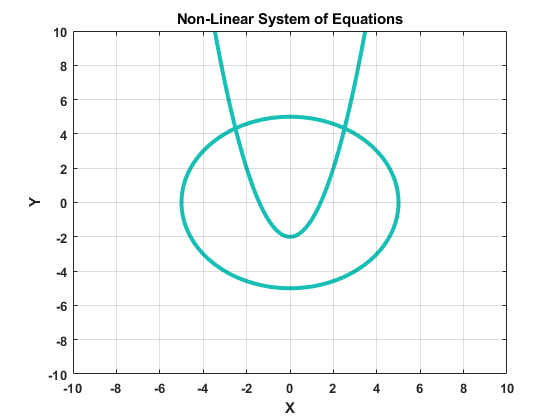
\includegraphics[width=0.35\textwidth]{ass3n_problem1_system.png}
%\caption{Non-linear system for problem \#1.}
%\label{fig:ass3n-prob1-system}
%\end{wrapfigure}




\begin{enumerate}

\item Consider a non-linear system of equations comprising the following functions:

%\begin{adjustbox}{minipage={\linewidth}, valign=t}
%\begin{wrapfigure}{t}{0.4\linewidth}
%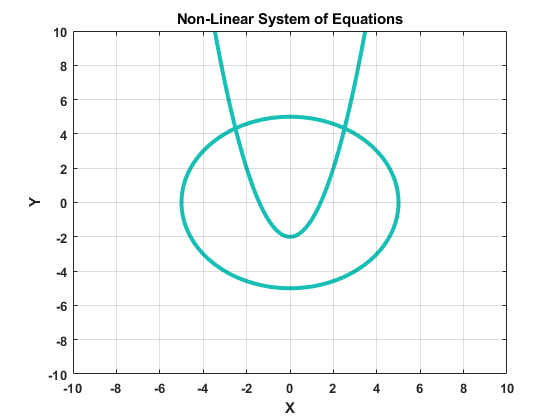
\includegraphics[width=\linewidth]{ass3n_problem1_system.png}
%\caption{Non-linear system for problem \#1.}
%\label{fig:ass3n-prob1-system}
%\vspace{-1.65\baselineskip}
%\end{wrapfigure}
%\vspace*{0.25em}
%\blindtext
%\end{adjustbox}

\begin{align*}
f(x,y) &= x^2 + y^2 - 25 = 0 \\
g(x,y) &= x^2 - y - 2 = 0
\end{align*}
Create a function to carry out Newton's method for finding a root for this system of non-linear equations.  The function should have the signature: \lstinline[style=myMatlab]{Xs = NewtonSystemSol(Fun, Jac, Xo, Tol, MaxIt)} where \lstinline[style=myMatlab]{Xs} is a root, \lstinline[style=myMatlab]{Fun} and \lstinline[style=myMatlab]{Jac} are handles to the system of functions to be solved and the Jacobian matrix, respectively.  \lstinline[style=myMatlab]{Xo} is an initial estimate of the root, \lstinline[style=myMatlab]{Tol} is the error tolerance and \lstinline[style=myMatlab]{MaxIt} is the maximum number of iterations to perform.  The error tolerance should be based on the relative change of each component of the estimated root. \lstinline[style=myMatlab]{Tol} should be set to $1 \times 10^{-9}$, \lstinline[style=myMatlab]{MaxIt} should be set to 25, and you should use \lstinline[style=myMatlab]{Xa = [2.5,2.5]} to find the root in the upper right-hand quadrant of the coordinate system.



\end{enumerate}
\vspace{1.0cm}



\begin{enumerate}[resume]
\item A coating on a panel surface is cured by radiant energy from a heater. The temperature of the coating is determined by radiative and convective heat transfer processes.  If the radiation is treated as diffuse and gray, the following non-linear system of equations determine the unknowns: $J_h$, $T_h$, $J_c$, and $T_c$.
\begin{align*}
5.67 \times 10^{-8} T^4_{c} + 17.41 T_c - J_c &= 5188.18 \\
J_c - 0.71 J_h + 7.46 T_c &= 2352.71 \\
5.67 \times 10^{-8} T^4_{h} + 1.865 T_h - J_h &= 2250 \\
J_h - 0.71 J_c + 7.46 T_h &= 11093
\end{align*}
Use MATLAB's built-in function \lstinline[style=myMatlab]{fsolve} to find values of $J_h$, $T_h$, $J_c$ and $T_c$ that satisfy this system of equations.  Use \lstinline[style=myMatlab]{optimoptions()} to set the maximum iterations at 50, and the \lstinline[style=myMatlab]{'StepTolerance'} to $1 \times 10^{-9}$.  For a starting value, use $T_c = T_h = 298$, $J_c = 3000$ and $J_h = 5000$.


\vspace{2.0cm}

\item Referring to Problem \#2 above, if you were to solve that system of equations using Newton's method, you would need to determine the Jacobian matrix.  Write down a symbolic version of the Jacobian matrix.

\vspace{2.0cm}

\item Solve the following system of equations using the Gauss elimination method.
\begin{align*}
2x_1 + x_2 - x_3 &= 1\\
x_1 + 2x_2 + x_3 &= 8\\
-x_1 + x_2 - x_3 &= -5\\
\end{align*}

\end{enumerate}


\vspace{2.0cm}

\begin{enumerate}[resume]
\item The axial force, $F_i$, in each of the 13-members of the pin-connected truss (add figure) can be calculated by solving the following system of 13 equations:

\begin{align*}
F_2 + 0.707 F_1 &= 0 \\
F_3 - 0.797 F_1 - 2000 &= 0 \\
0.7071 F_1 + F_4 + 6229 &= 0 \\
-F_2 + 0.659F_5 + F_6 &= 0 \\
-F_4 - 0.753 F_5 - 600 &= 0 \\
-F_3 - 0.659 F_5 + F_7 &= 0 \\
0.753 F_5 + F_8 &= 0 \\
-F_6 + 0.659 F_9 + F_{10} &= 0 \\
-F_8 - 0.753 F_9 - 800 &= 0 \\
-F_7 -0.659 F_9 + F_{11} &= 0 \\
0.753F_9 + F_{12} - 2429 &= 0 \\
-F_{10} + 0.707 F_{13} &= 0 \\
-F_{12} - 0.7071 F_{13} - 600 &= 0
\end{align*}




\end{enumerate}

\end{fullwidth}

\chapter{Lecture 9 - LU Factorization}
\label{ch:lec9n}
\section{Objectives}
The objectives of this lecture are to:
\begin{itemize}
\item Quantify the computational work of Gauss elimination.
\item Describe the LU factorization.
\item Demonstrate how to use the LU factorization for solving systems of equations.
\end{itemize}
\setcounter{lstannotation}{0}

\section{Computational Work of Gauss Elimination}

Throughout this course we have taken a rather crass approach to the amount of work done by the computer.  This reflects, in part, a basic reality that for many undergraduate students of engineering, most of the computer-based work comprises time that students spend writing and debugging code.  The amount of time that the computer actually spends executing the program, in many cases, is trivial.  

Looking ahead to some of the numerical methods that will be learned in this course, the situation will change.  Programs that analyze initial boundary value problems based on the finite difference method or finite element method will need to solve large systems of linear or non-linear equations.  These systems of equations are often large---it is not unusual to have millions of equations and unknowns---and the time that the computer spends assembling and solving these equations becomes significant.  Applications of this type are so important that modern high performance computing systems are regularly benchmarked based on how fast they can solve such problems.\cite{HPL,top500}     

In this section will will undertake a high-level analysis of the computational work required to perform Gauss elimination.  We will break this analysis into two parts: a) the forward elimination phase; and b) the back-substitution phase.

\subsection{Forward Elimination}
MATLAB code for the forward elimination phase is shown in the listing below:
\begin{lstlisting}[style=myMatlab]
for j = 1:n-1 /*!\annotation{lst:ann9n-1}!*/
    for i = (j+1):n /*!\annotation{lst:ann9n-2}!*/
        m = A(i,j)/A(j,j); % calculate pivot /*!\annotation{lst:ann9n-3}!*/
        A(i,j:n) = A(i,j:n) - m*A(j,j:n); /*!\annotation{lst:ann9n-4}!*/
        
        b(i) = b(i) - m*b(j); % update the right hand side /*!\annotation{lst:ann9n-5}!*/
    end
end
\end{lstlisting}

\vspace{0.1cm}

\noindent \ref{lst:ann9n-1} The outer loop, \lstinline[style=myMatlab]{for j=1:n-1...end}, will be traversed $\mathcal{O}(n)$ times.\sidenote{Here we adopt \emph{``Big oh''} notation.  It is used to charactarize the complexity and running time of an algorithm in asymptotic fashion.  So in this case, $\mathcal{O}(n)$ means that, as $n\to\infty$, the running time of this part of the code increases linearly with $n$.  Small details like constant factors are ignored.  It also means that lower order terms get ignored.  For example, a function that requires $n^3 + n^2 + n$ calculations would be characterized as $\mathcal{O}(n^3)$ since, as $n\to\infty$, the $n^2$ and $n$ terms become insignificant relative to $n^3$.}

\vspace{0.25cm} 

\noindent \ref{lst:ann9n-2} The inner loop, \lstinline[style=myMatlab]{for i=(j+1):n...end}, also will be traversed $\mathcal{O}(n)$ times.  

\vspace{0.25cm}

\noindent \ref{lst:ann9n-3} This line performs one floating point operation (FLOP) to calculate the pivot.

\vspace{0.25cm}

\noindent \ref{lst:ann9n-4} This line performs $\mathcal{O}(n)$ floating point operations.  These include multiplication of a vector by a scalar and vector addition.

\vspace{0.25cm}

\noindent \ref{lst:ann9n-5} This line performs two FLOPs: scalar multiplication and scalar addition.

\vspace{0.25cm}

\noindent Overall the forward-elimination part of the algorithm requires: $\mathcal{O}(n) \times \mathcal{O}(n) \times \mathcal{O}(n)$ operations to traverse the two nested loops and carry out the operations inside. The asymptotic operation count is thus: $\mathcal{O}(n^3)$.

\subsection{Back-Substitution}
MATLAB code for the back-substitution phase is shown in the listing below:
\begin{lstlisting}[style=myMatlab]
x = nan(n,1); 
for i = n:-1:1    /*!\annotation{lst:ann9n-6}!*/
   x(i) = (b(i) - ...    /*!\annotation{lst:ann9n-7}!*/
       A(i,(i+1):n)*x((i+1):n))/A(i,i);    
end
\end{lstlisting}

\vspace{0.25cm}

\noindent \ref{lst:ann9n-6} This loop is traversed $\mathcal{O}(n)$ times.

\vspace{0.25cm}

\noindent \ref{lst:ann9n-7} This line performs $\mathcal{O}(n)$ FLOPS for vector dot product, scalar addition and division.

\vspace{0.25cm} 

\noindent Overall, the back-substitution part of the algorithm requires: $\mathcal{O}(n) \times \mathcal{O}(n)$ operations; the asymptotic operation count is therefore: $\mathcal{O}(n^2)$.

\vspace{4.25cm}

\newthought{Taken together}, the entire Gauss elimination algorithm requires $\mathcal{O}(n^3) + \mathcal{O}(n^2)$ operations for a total asymptotic complexity of: $\mathcal{O}(n^3)$.  For large enough matrices, if you double the matrix size, the computer will need to perform a factor of $\approx 2^3$ more floating point operations and, roughly speaking, can be expected to take $2^{3}$ times as long. This is shown in Figure \ref{fig:lec9n-compute-vs-n}.
\begin{marginfigure}
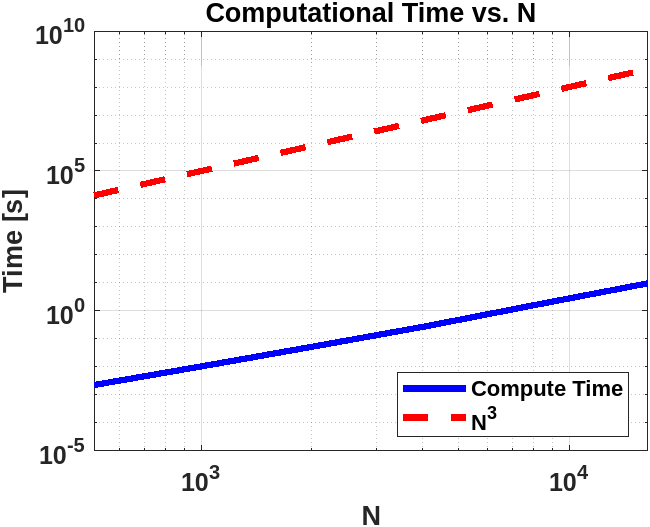
\includegraphics{lec9n_compute_vs_n.png}
\caption{Computing time vs. $n$ for Gauss elimination.}
\label{fig:lec9n-compute-vs-n}
\end{marginfigure}

\setcounter{lstannotation}{0} % do a re-set of the counter
\section{LU Factorization}
One problem with the Gauss elimination algorithm as described so far is this:  if you want to repeat the solution with a different right-hand-side, you would need to repeat all of the work you had just done.  We will not cover it in this class, but one possible solution to this problem is to devise an algorithm like Gauss elimination\sidenote{The Gauss-Jordan elimination does this.} that, in addition to solving the problem for the unknown vector $x$, also finds $A^{-1}$, the inverse of $A$.  With the inverse, we could find $x$ for a new right hand side with a simple matrix-vector multiplication.
\begin{align*}
Ax &= b \\
A^{-1}Ax &= A^{-1}b \\
Ix &= A^{-1}b \\
\Rightarrow x &= A^{-1}b
\end{align*}
As asymptotic analysis will readily show, matrix multiplication has $\mathcal{O}(n^2)$ complexity, so we can re-compute $x$ for any new $b$ in a small fraction of the time that it would take to re-perform Gauss elimination.  
We will not do this, however.  Instead we will perform a \emph{factorization} of $A$ in such a way that we can solve the linear system, $Ax=b$, with $\mathcal{O}(n^2)$ operations, for any new right hand side, $b$. This is called the \emph{LU factorization} and it is both faster and more-accurate (in floating point arithmetic) than finding the matrix inverse.\cite{higham-matrix-inverse} 

The LU factorization decomposes an invertible matrix into:
\begin{itemize}
\item A lower triangular matrix L; and
\item an upper triangular matrix U
\end{itemize}
such that $A = LU$.  It turns out that, while carrying out the Gauss elimination algorithm we actually computed th elements of the LU factorization:
\begin{equation*}
\underbrace{
\bracketMatrixstack{
a_{11} & a_{12} & a_{13} & a_{14} \\
a_{21} & a_{22} & a_{23} & a_{24} \\
a_{31} & a_{32} & a_{33} & a_{34} \\
a_{41} & a_{42} & a_{43} & a_{44}
}
}_{
A
}
=
\underbrace{ 
\bracketMatrixstack{
1 & 0 & 0 & 0 \\
m_{21} & 1 & 0 & 0 \\
m_{31} & m_{32} & 1 & 0 \\
m_{41} & m_{42} & m_{43} & 1
}
}_{
L
}
\underbrace{
\bracketMatrixstack{
a_{11} & a_{12} & a_{13} & a_{14} \\
0 & a^{\prime}_{22} & a^{\prime}_{23} & a^{\prime}_{24} \\
0 & 0 & a^{\prime \prime}_{33} & a^{\prime \prime}_{34} \\
0 & 0 & 0 & a^{\prime \prime \prime}_{44}
}
}_{
U
}
\end{equation*}
Where the pivots comprise the elements of $L$ and the transformed coefficient matrix after Guass elimination is $U$. In a sense, all we have to do is ``write down what we are doing'' during the forward elimination portion of Gauss elimination in order to obtain the LU factorization.  This is illustrated in the MATLAB code below: \marginnote[2.0cm]{

\ref{lst:ann9n-1} Initialize $U = A$. Carry out operations on $U$ just as you did for $A$ in forward elimination phase of Gauss elimination.

\vspace{0.25cm}

\ref{lst:ann9n-2} Compute the privot and store in $L$.

\vspace{0.15cm}

\ref{lst:ann9n-3} Carry out elimination step on $U$.

}
\begin{lstlisting}[style=myMatlab]
function [L,U] = LU_Factor(A)
% LU factorization without pivoting

[m,n] = size(A); % get rows and columns of A
U = A;  /*!\annotation{lst:ann9n-1}!*/
L = eye(m,n); % constructor for identity matrix.

for k = 1:(m-1)
    for j = (k+1):m
        L(j,k) = U(j,k)/U(k,k); /*!\annotation{lst:ann9n-2}!*/
        U(j,k:m) = U(j,k:m) - L(j,k)*U(k,k:m); /*!\annotation{lst:ann9n-3}!*/
    end
end
end
\end{lstlisting}

Now that we have the LU factorization, suppose we want to solve a new linear system with the same matrix $A$ but a new right hand side: $c$.
\begin{align*}
Ax &= c \\
LUx &= c \\
\end{align*}
Let us denote $y = Ux$ and solve:
\begin{equation*}
Ly = c
\end{equation*}
Since $L$ is lower triangular, we can solve for $y$ using \emph{forward substitution}.  MATLAB code for forward substitution is presented below:
\begin{lstlisting}[style=myMatlab]
function y = ForwardSub(L,c)
n = length(c);
y(1,1) = c(1)/L(1,1);
for i = 2:n
   y(i,1)=(c(i)-L(i,1:(i-1))*y(1:(i-1),1))./L(i,i); 
end
end
\end{lstlisting}
Then we can obtain $x$ by solving $Ux = y$ with backward substitution.  MATLAB code for backward substitution is presented below:
\begin{lstlisting}[style=myMatlab]
function x = BackwardSub(U,y)
n = length(y);
for i = n:-1:1
   x(i,1)=(y(i)-U(i,(i+1):n)*x((i+1):n,1))/U(i,i); 
end
end
\end{lstlisting}
which you should recognize as being the same as the backward substitution step used in Gauss elimination.

The MATLAB listing below puts this all together for a simple example:
\begin{lstlisting}[style=myMatlab]
A = [4, -2, -3, 6;
    -6, 7, 6.5, -6;
     1, 7.5, 6.25, 5.5;
    -12, 22, 15.5, -1];
        
b = [12;
    -6.5;
     16;
     17];

[L,U] = LU_Factor(A);
y = ForwardSub(L,b);
x = BackwardSub(U,y);

%% Local functions
function [L,U] = LU_Factor(A)
% LU factorization without pivoting
[m,n] = size(A); % get rows and columns of A
U = A;
L = eye(m,n); % constructor for identity matrix.

for k = 1:(m-1)
    for j = (k+1):m
        L(j,k) = U(j,k)/U(k,k);
        U(j,k:m) = U(j,k:m) - L(j,k)*U(k,k:m);
    end
end
end

function y = ForwardSub(L,c)
n = length(c);
y(1,1) = c(1)/L(1,1);
for i = 2:n
   y(i,1)=(c(i)-L(i,1:(i-1))*y(1:(i-1),1))./L(i,i); 
end
end

function x = BackwardSub(U,y)
n = length(y);
for i = n:-1:1
   x(i,1)=(y(i)-U(i,(i+1):n)*x((i+1):n,1))/U(i,i); 
end
end
\end{lstlisting}
\index{permutation matrix} 
\section{LU Factorization with Pivoting}
As we saw in the last lecture, pivoting is an essential operation if you want to accurately solve relevant matrices. Pivot operations can be captured in a \emph{permutation matrix}.  Switching rows in a vector or a matrix is equivalent to multiplying by the identiy matrix with columns switched.  For example, when pivoting is performed on the matrix example from Lecture 8, the final permuted row ordering is: 
\begin{equation*}
\left[ \begin{matrix} 1 & 2 & 3 & 4 \end{matrix} \right] \rightarrow \substack{\text{ Swapped } \\ \text{1\&4}} \rightarrow \substack{\text{ Swapped } \\ \text{2\&3}} \rightarrow \substack{\text{ Swapped } \\ \text{3\&4}} \rightarrow \left[\begin{matrix}4 & 3 & 1 & 2 \end{matrix} \right]
\end{equation*}
We can represent this as a permutation matrix, $P$, constructed as the idenitty matrix with columns correspondingly reordered.
\begin{equation*}
P = 
\bracketMatrixstack{
0 & 0 & 0 & 1 \\
0 & 0 & 1 & 0 \\
1 & 0 & 0 & 0 \\
0 & 1 & 0 & 0
}
\end{equation*}
To solve a system of equations with LU-factoring with pivoting:
\marginnote{ 

\vspace{0.80cm}

Perform LU factorization on $PA$.

\vspace{0.25cm}

Permute $b$.

\vspace{0.25cm}

Forward solve for $y$.

\vspace{0.25cm}

Backward solve for $x$.
}
\begin{align*}
PA &= LU \\
b_p &= Pb \\
Ly &= b_p \\
Ux &= y
\end{align*}
In MATLAB code:
\begin{lstlisting}[style=myMatlab]
[L,U] = LU_Factor(P*A);
bp = P*b;
y = ForwardSub(L,bp);
x_p = BackwardSub(U,y);
\end{lstlisting}

\chapter{Lecture 10 - Legendre's Equation}
\label{ch:lec10}
\section{Objectives}
The objectives of this lecture are:
\begin{itemize}
\item Illustrate the use of the power series method to solve Legendre's equation. 
\item Introduce some of the properties of Legendre polynomials.
\end{itemize}

\section{Legendre's Equation}
The following 2\textsuperscript{nd}-order linear, homogeneous ODE is known as Legendre's equation:
\begin{equation}
\left(1-x^2 \right)u^{\prime \prime}-2xu^{\prime} + m(m+1)u = 0 
\label{eq:legendre}
\end{equation}
where $m$ is a constant.

\newthought{First we will} put Equation \ref{eq:legendre} into standard form:
\begin{equation*}
u^{\prime \prime} - \frac{2x}{\left( 1-x^2 \right)}u^{\prime} + \frac{m(m+1)}{\left(1-x^2 \right)}u = 0
\end{equation*}
We should immediately note that $P(x) = \frac{2x}{\left( 1-x^2 \right)}$ and $Q(x) = \frac{m(m+1)}{\left(1-x^2 \right)}$ are singular (and thus not analytic) at $x=\pm1$. Recall from Theorem \ref{thm:existence-of-power-series-solutions} that $P(x)$ and $Q(x)$ must be analytic for power series solutions to exist.
\newthought{We will restrict} our attention to the interval $x \in (-1,1)$ and use the power series method to find a solution.  Inserting our assumed power series solution into Equation \ref{eq:legendre} gives us:
\begin{fullwidth}
\begin{align*}
\left(1-x^2 \right)\sum\limits_{n=2}^{\infty} n(n-1)c_nx^{n-2} - 2x\sum\limits_{n=1}^{\infty} n c_nx^{n-1} + m(m+1)\sum\limits_{n=0}^{\infty}c_nx^n & = 0 \\
\underbrace{\sum\limits_{n=2}^{\infty}n(n-1)c_nx^{n-2}}_{x^0} - \underbrace{\sum\limits_{n=2}^{\infty}n(n-1)c_nx^n}_{x^2} - \underbrace{\sum\limits_{j=1}^{\infty}2nc_nx^n}_{x^1} + \underbrace{m(m+1)\sum\limits_{n=0}^{\infty}c_nx^n}_{x^0} &= 0
\end{align*}
\end{fullwidth}
where we see that all terms with order lower than $x^2$ need to be pulled outside of their summations so all four can be in phase.
\begin{fullwidth}
\begin{multline*}
(2)(1)c_2 + (3)(2)c_3x + \underbrace{\sum\limits_{n=4}^{\infty}n(n-1)c_nx^{n-2}}_{\substack{k=n-2 \\ n=k+2}} - \underbrace{\sum\limits_{n=2}^{\infty}n(n-1)c_nx^{n}}_{\substack{k=n \\ n=k}} - (2)(1)c_1x - \underbrace{\sum\limits_{n=2}^{\infty}2nc_nx^n}_{\substack{k=n \\ n=k}} + \dots \\
m(m+1) \left(c_0 + c_1x\right) + m(m+1)\underbrace{\sum\limits_{n=2}^{\infty}c_n x^n}_{\substack{k=n \\ n=k}} = 0
\end{multline*}
Combining terms outside of the summations and making the indicated substitutions to combine the summations we get:
\begin{multline*}
\left[m(m+1)c_0 + 2c_2 \right] + [\underbrace{(m(m+1)-2)}_{(m-1)(m+2)}c_1 + 6c_3]x + \dots \\
\sum\limits_{k=2}^{\infty}[(k+2)(k+1)c_{k+2} \underbrace{- k(k-1)c_k - 2kc_k + m(m+1)c_k}_{(m-k)(m+k+1)c_k}]x^k = 0
\end{multline*}
\end{fullwidth}
Applying the indicated algebraic simplifications leads us finally to:\marginnote{\textbf{Note:} Obviously this is a tedious business.  Be careful and make sure you understand each manipulation.}
\begin{multline*}
[m(m+1)c_0+2c_2] + [(m+1)(m+2)c_1 + 6c_3]x + \cdots \\
\sum\limits_{k=2}^{\infty}[(k+2)(k+1)c_{k+2} + (m-k)(m+k+1)c_k]x^k=0
\end{multline*}
The next steps are to find formulas for the power series coefficients, $c_n$, so that the combined coefficient for each power of $x$ in the equation above equals zero. For the constant term $(x^0)$ we have:
\begin{equation*}
c_2 = \frac{-m(m+1)c_0}{2}
\end{equation*}
For the linear term $(x^1)$ we get:
\begin{equation*}
c_3 = \frac{-(m-1)(m+2)}{6}c_1
\end{equation*}
For all other powers of $x$, we get a 2-term recurrence:
\begin{equation*}
c_{k+1} = \frac{-(m-k)(m+k+1)}{(k+2)(k+1)}c_k
\end{equation*}
\begin{margintable}
\begin{tabular}{l}
$k=2$ \\
$c_4 = \frac{-(m-2)(m+3)}{(4)(3)}c_2 = \frac{(m-2)(m+3)m(m+1)}{(4)(3)(2)}c_0$ \\
$k=3$ \\
$c_5 = \frac{-(m-3)(m+4)}{(5)(4)}c_3 = \frac{(m-3)(m+4)(m-1)(m+2)}{(5)(4)(3)(2)}c_1$ \\
\end{tabular}
\end{margintable}
\noindent Organizing these into two solutions we get:
\begin{align*}
u_1(x) &= c_0\left[1 + \frac{c_2}{c_0}x^2 + \frac{c_4}{c_0}x^4 + \cdots \right] \\
&= c_0 \left[1-\frac{m(m+1)}{2!}x^2 + \frac{(m-2)(m+3)m(m+1)}{4!}x^4 + \cdots  \right] \\
u_2(x) &= c_1\left[x + \frac{c_3}{c_1}x^3 + \frac{c_5}{c_1}x^5 + \cdots \right] \\
&= c_1\left[x - \frac{(m-1)(m+2)}{3!}x^3+\frac{(m-3)(m+4)(m-1)(m+2)}{5!}x^5 + \cdots \right]
\end{align*}
So far what we have is messy but, when dealing with power series solutions, messiness is the order of the day.  One point that we have quietly left to the side is whether or not we expect this (so called) power series solution  to converge.\marginnote{\textbf{Reminder:} If the power series that we purport to be a solution to the differential equation is divergent than we really have nothing.}

One way that we can permanently leave these questions to the side is if $m$ is an integer.  Notice that if $m=0$ or is an even integer,\sidenote{i.e. If $m$ is even then $u_1(x)$ is a polynomial.} $u_1(x)$ terminates with a finite number of terms. Similarly with $u_2(x)$ in the case that $m$ is an odd integer. 

\newthought{These polynomial solutions}, where $m$ is an integer, are referred to as Legendre polynomials.  Legendre polynomials have several important applications; our primary use for them will be when solving equations in spherical coordinate systems.

\section{Important Properties of Legendre Polynomials}
Legendre polynomials are solutions to Legendre's equation where $m$ is an integer:
\begin{equation*}
\left(1-x^2 \right)u^{\prime \prime} - 2xu^{\prime} + m(m+1)u = 0
\end{equation*}

By convention the leading coefficients are chosen such that Legendre polynomials have a maximum value of 1 on the interval $x\in[-1,1]$.  

\begin{margintable}
\begin{tabular}{c | c}
$P_0(x) = 1$ & $P_1(x) = x$ \\\hline
$P_2(x) = \frac{1}{2}(3x^2-1)$ & $P_3(x) = \frac{1}{2}(5x^3-3x)$ \\
\end{tabular}
\caption{The first four Legendre Polynomials}
\label{tab:Legendre-poly}
\end{margintable}
The first few Legendre Polynomials are shown in the Table \ref{tab:Legendre-poly}. Higher order Legendre polynomials can be constructed using a three-term recurrence relation shown in Equation \ref{eq:legendre-three-term}:
\begin{equation}
(n+1)P_{n+1}(x) - (2n+1)xP_n(x) + nP_{n-1}(x) = 0
\label{eq:legendre-three-term}
\end{equation}

\vspace{4.0cm}

Some other properties include:

\begin{align*}
P_n(-x) &= (-1)^nP_n(x) \\
P_n(1) &= 1 \\
P_n(-1) &= (-1)^n \\
P_n(0) &= 0 \text{ for } n\in{\text{odd}} \\
P_n^{\prime}(0) &=0 \text{ for } n\in{\text{even}}
\end{align*}
\begin{marginfigure}
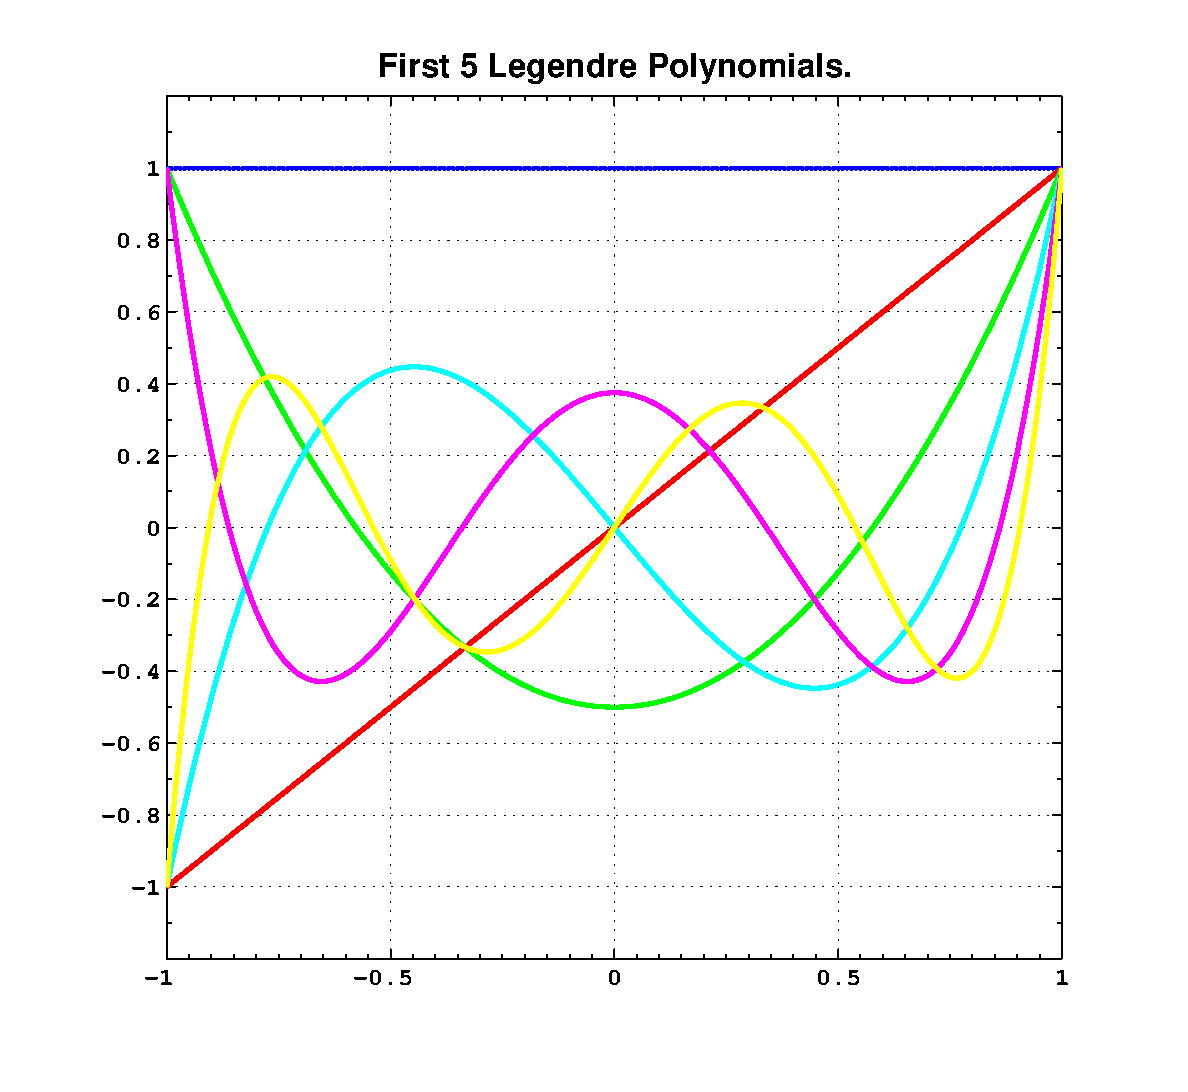
\includegraphics{LegendrePolyPlot.eps}
\caption{Legendre Polynomials of order 0 through 5.}
\label{fig:legendre-poly-plot}
\end{marginfigure}
A plot of the first few Legendre Polynomials is shown in Figure \ref{fig:legendre-poly-plot}.


\newthought{The last property} that we will mention here, and that we will make use of extensively in this course, is the \emph{orthogonality} property of Legendre polynomials.\marginnote[1.0cm]{Orthogonality of functions is analogous to orthogonality of vectors.  Two functions, $f_1(x)$ and $f_2(x)$ are orthogonal on an interval $x\in[a,b]$ if $\int_a^b f_1(x)f_2(x) \ dx = 0$.}
Legendre polynomials are orthogonal over the interval $x \in [-1,1]$.  This mean that Equation \ref{eq:legendre-orthogonality} holds:
\begin{equation}
\int_{-1}^{1} P_n(x) P_m(x) \ dx = 
\begin{cases}
0, \ \ n \ne m \\
\frac{2}{n+1}, \ \ n = m \\
\end{cases}
\label{eq:legendre-orthogonality}
\end{equation}


\chapter{Lecture 11 Sparse Matrices and Iterative Solution Methods}
\label{ch:lec11n}
\section{Objectives}
The objectives of this lecture are to:
\begin{itemize}
\item Describe sparse matrices and their importance in scientific computing.
\item Introduce iterative solution methods.
\item Show some examples.
\end{itemize}
\setcounter{lstannotation}{0}

\section{Introduction}
Up to this point we have discussed a handful of methods for solving linear systems of equations.  We studied Gauss elimination with and without pivoting; LU factorization which, to be sure, is basically the same as Gauss elimination.  We also learned a little bit about the array of solution methods that are used in MATLAB's built-in tools for linear equations such as the QR factorization and LDL and Cholesky factorizations.  These are fundamental methods that should be in the toolbox of every engineer.

There are practical situations where these direct solution methods for linear equations are not suitable.  Physical conservation laws that are encoded in partial differential equations, discretized and solved using methods like the finite element method (FEM) and finite volume method (FVM) result in large systems of linear equations.  A high-resolution simulation will routinely require upwards of $10^5$ degrees of freedom\sidenote{In this context, the number of \emph{degrees of freedom} can be interpreted to refer to the length of a vector describing the unknown function.} to adequately resolve the physics of interest such as: the flow field around an automobile to estimate drag forces; stress and strain distribution within a complex structural component to ensure material failure limits are not exceeded; or the component temperature in the vicinity of a weld process.

Just \emph{storing} the matrices used to represent these linear systems---something, for example, like a $10^5 \times 10^5$ matrix\sidenote[][-1.25cm]{Such a matrix has $10^{10}$ entries.  If each entry is represented with a double-precision floating point number (8 bytes each), that adds up to roughly 80 Gigabytes of memory just to \emph{store} the matrix.}---requires us to take a new approach from what we have described up to now.  Likewise solving the systems to find the unknown vectors---whether the vector represents temperature, pressure, a velocity component, or a component of material displacement---requires new techniques.

\section{Sparse Matrices}

Matrices that arise as part of a finite difference method or finite element method are almost always \emph{sparse}.  This means that for every row of the matrix, corresponding to a linear equation pertaining to a single degree of freedom, most of the entries are equal to zero.  

\begin{marginfigure}[-3.75cm]
%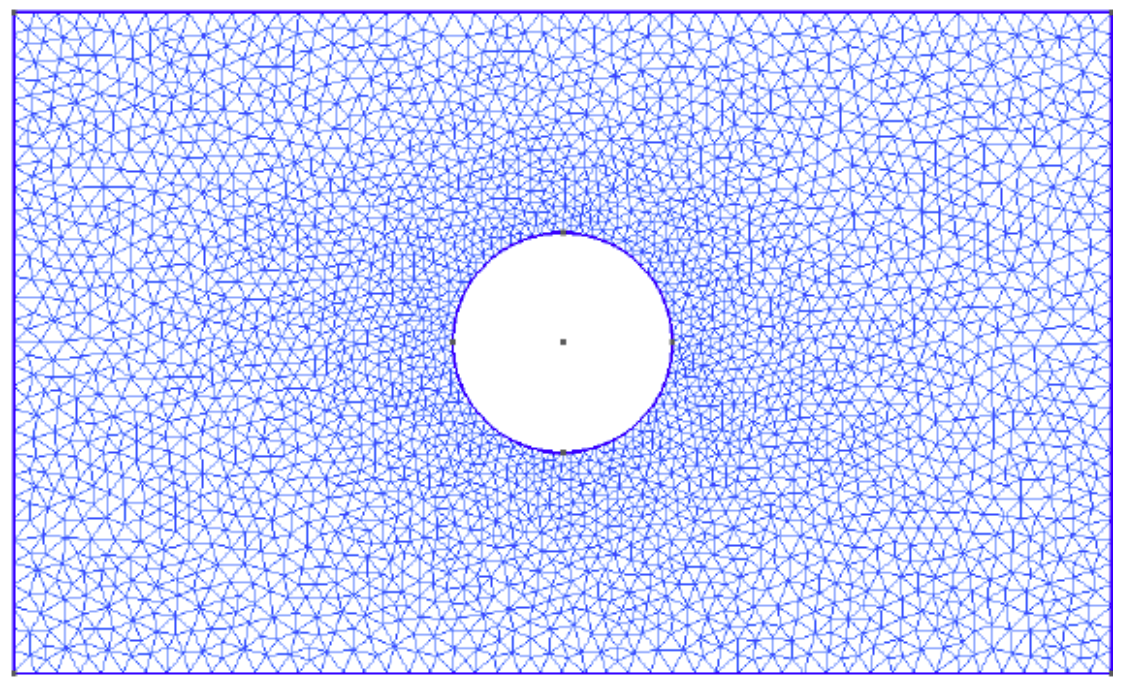
\includegraphics{lec11n-mesh.png}
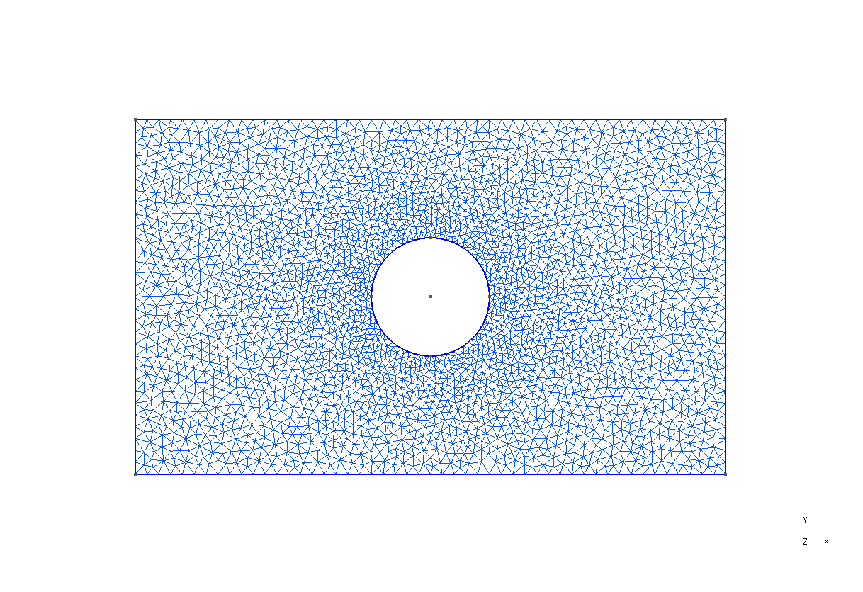
\includegraphics{discretization.eps}
\caption{A triangular mesh for a finite element method analysis of the transient heat equation.}
\label{fig:lec11n-mesh}
\end{marginfigure}
As an example, consider a finite element discretization of the transient heat equation on a domain that is rectangular in shape, but with a hole in the middle.  The mesh is depicted in Figure \ref{fig:lec11n-mesh}. The governing equation is shown in Equation \ref{eq:lec11n-transient-heat}:
\begin{equation}
\frac{k}{\rho c_p}\frac{\partial u}{\partial t} = \nabla^2 u + S
\label{eq:lec11n-transient-heat}
\end{equation}
where $k$ is the thermal conductivity, $\rho$ is density, $c_p$ is the specific heat, $S$ corresponds to a constant uniform heat source, $u$ is the temperature, and $t$ is time. In the finite element method, this equation and specified boundary conditions are translated into a linear system of equations:
\begin{equation*}
Au = b
\end{equation*} 
\begin{marginfigure}[-6.0cm]
%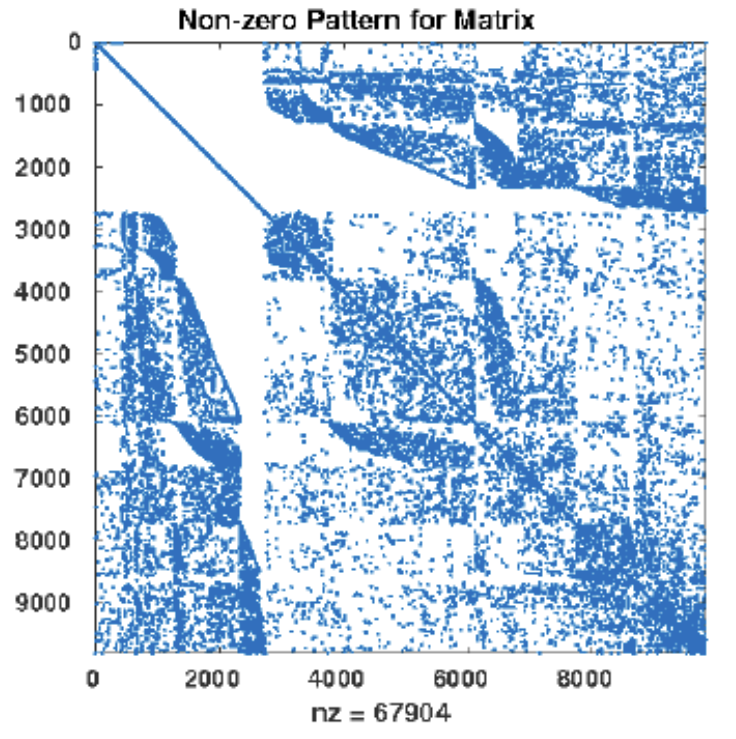
\includegraphics{lec11n-spy1.png}
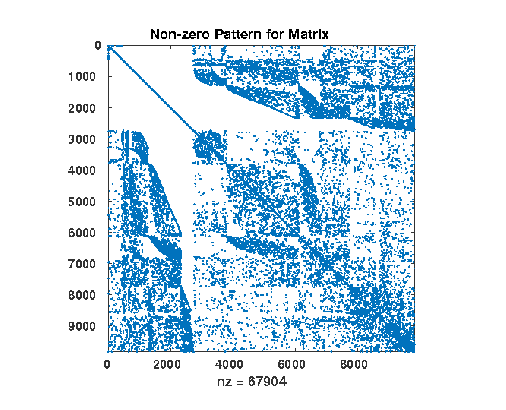
\includegraphics{Thermal_9824.eps}
\caption{Non-zeros in linear system for transient heat conduction.}
\label{fig:lec11n-spy1}
\end{marginfigure}
The non-zero structure of this system of equations can be observed using MATLAB's built-in function \lstinline[style=myMatlab]{spy(A)}, and the result is shown in Figure \ref{fig:lec11n-spy1}. The system of equations has 9824 nodes, each with a single degree of freedom.  The resulting $9824 \times 9824$ matrix $A$ has a total of 67,904 non-zero entries; an average of about 8 non-zero elements per equation.\sidenote[][-3.0cm]{Bottom Line Up Front: this number of non-zeros per row is typical for two-dimensional systems with linear, triangular elements.  The number of non-zeros per equation for the FEM or FVM depends on a number of factors: a) number of degrees of freedom per node; b) the number of spatial dimensions; c) the number of internal degrees of freedom for each finite element, among other factors.  This will be discussed in detail in later lectures on finite element methods.  } This pattern, which is typical for such matrices, can be exploited by only storing and carrying out arithmetic with the non-zero entries of the matrix.  

There are a number of sparse-matrix storage formats in use.  MATLAB uses the compressed-sparse-column (CSC) storage format.\cite{gilbert1992sparse}  If there are $nnz$ non-zero entries in a $n \times n$ sparse array, MATLAB stores one (double precision) vector of length $nnz$ with the non-zero values---call this vector: \lstinline[style=myMatlab]{ENTRY}; another vector of integers of length $nnz$---call this vector: \lstinline[style=myMatlab]{ROW}---with the row-number for each non-zero; and a third vector of integers of length $n+1$---call this vector: \lstinline[style=myMatlab]{COL}---that stores the index (from the \lstinline[style=myMatlab]{ENTRY} array) of the first non-zero from each column and terminated with $nnz+1$.  An example of this format is shown in Figure \ref{fig:lec11n-csc}. \begin{marginfigure}
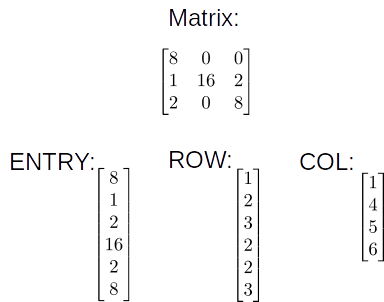
\includegraphics{CSC-example.png}
\caption{Example sparse matrix in Compressed Sparse Column format.}
\label{fig:lec11n-csc}
\end{marginfigure} The total storage required is $nnz \times 8$ bytes for the \lstinline[style=myMatlab]{ENTRY} array + $nnz \times 4$ bytes for the \lstinline[style=myMatlab]{ROW} array + $(n+1) \times 4$ bytes for the \lstinline[style=myMatlab]{COL} array.  In asymptotic notation, $\mathcal{O}(nnz+n)$ bytes of storage are required.  Contrast this with $\mathcal{O}(n^2)$ for dense matrices.  If $nnz << n$ the savings with sparse matrices is huge.  The key issues to keep in mind are these:\marginnote{In terms of FLOPs, sparse matrix calculations are slower.  Dense matrix algorithms are heavily optimized to make best use of the memory hierarchy of common computer architectures resulting in high computational intensity---calculations performed for each byte loaded from memory---and consequently achieve high performance.  Sparse matrix algorithms have lower computational intensity and the memory access patterns are harder to optimize for multi-threaded execution.  As a result, sparse matrix operations are relatively slow.  Readers are encouraged to experiment with MATLAB to get a better feel for the relative performance of dense and sparse matrix operations.}
\begin{enumerate}
\item Exploiting the sparsity of these matrices is not a performance enhancement, it is a necessity.  Simulations of practical interest often result in systems of equations that can \emph{only} be stored as a sparse matrix.
\item The resulting matrix, if it is to be solved, \emph{cannot} be solved by Gauss elimination related algorithms like LU-factorization.
\end{enumerate}

The reason for the second point is that, even for matrices that are sparse, the LU-factorization (or modified coefficient array for Gauss elimination) for that matrix usually is not sparse.  The forward elimination process common to both of the aforementioned techniques systematically destroys the sparsity pattern.  This effect is shown in Figure \ref{fig:lec11n-LandU}.
\begin{figure}[h!]
\subfloat[]{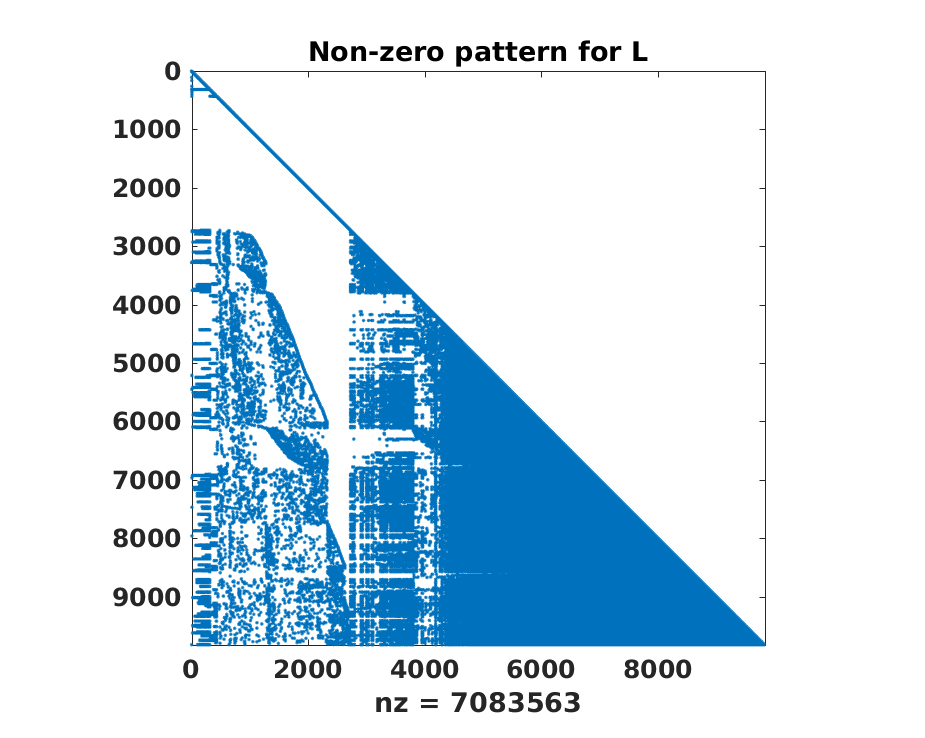
\includegraphics[width=2in]{Non_zero_L_thermal.eps}}
\subfloat[]{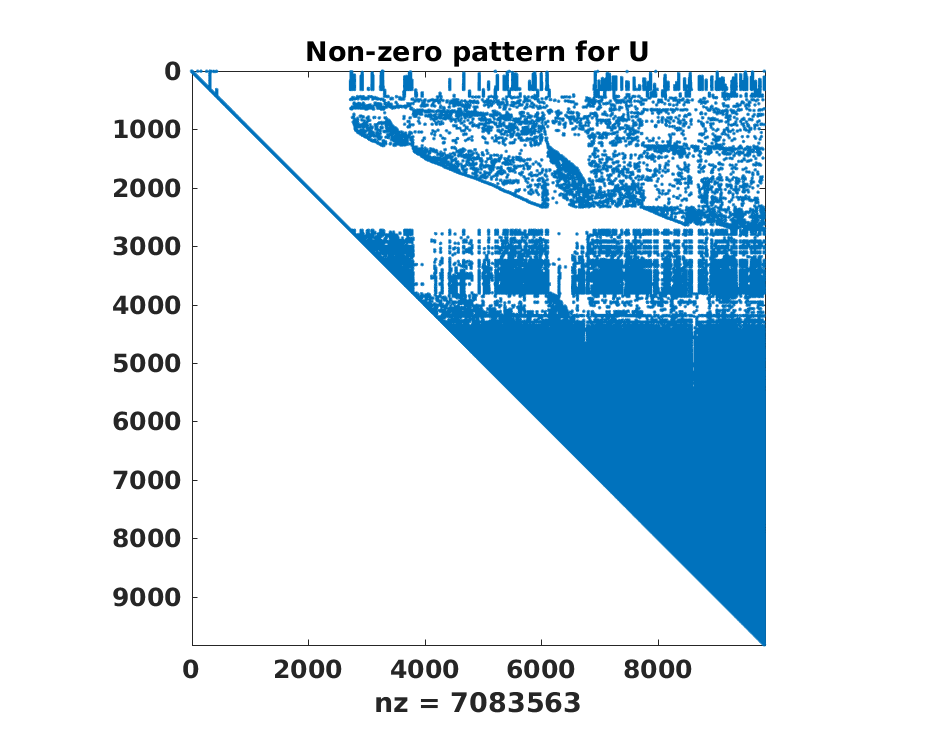
\includegraphics[width=2in]{Non_zero_U_thermal.eps}}
\label{fig:lec11n-LandU}
\caption[][3.0cm]{Sparsity pattern of L and U matrices from decomposition of A.}
\end{figure}

\noindent For the larger systems of equations that we want to solve for more interesting problems, this kind of fill-in defeats any benefit obtainable through use of sparse matrices.

\section{Iterative Solution Methods}

The fundamental idea of iterative methods for solving linear systems of equations is this: given an estimate of the solution, $x^{(k)}$, find a method to generate a new estimate, $x^{(k+1)}$, that is easy to compute and that ultimately converges to the solution of $Ax=b$.  Some of the methods that we will discuss in this lecture all involve \emph{splitting} the matrix $A$ into a decomposition $A=M-K$ with $M$ non-singular and very easy to invert.  If this is done, the iterative scheme is as follows:
\begin{align*}
Ax &= b \\
(M-K)x &= b \\
\rightarrow Mx &= Kx + b \\
\rightarrow x &= M^{-1}(Kx + b) \\
&= \underbrace{M^{-1}K}_{R}x + \underbrace{M^{-1}b}_{c}
\end{align*} \marginnote[-3.0cm]{\textbf{Note:} The matrix $R$ plays an important part in the mathematical theory of iterative methods. One relevent result is that if $$||R|| < 1$$ in some matrix norm, then the iterative method will converge. To the best of my knowledge, this is \emph{why} we carry out this business with splitting.}
The resulting iterative method is shown in Equation \ref{eq:lec11n-iterative-gen}:
\begin{equation}
x^{(k+1)} = Rx^{k} + c
\label{eq:lec11n-iterative-gen}
\end{equation}
where $k$ is the iteration number.

Instead of solving a system of equations by factoring the coefficient matrix, we create what we hope to be a convergent sequence of approximations to the solution by repeated matrix-vector multiplication.  Each matrix-vector multiplication operation takes, for dense matrices, $\mathcal{O}(n^2)$ operations.  Since the matrix $R$ is sparse and operations with zero entries of the matrix are eliminated, each matrix-vector multiplication takes only $\mathcal{O}(n)$ operations.

\subsection{Jacobi Iteration}

In this method, $M$ is defined to be the diagonal of $A$, and $K$ is the sum of the strictly lower and upper triangular portion of $A$.\cite{demmel1997applied}
\begin{align}
M &= \text{diag}(A) \\
K &= \tilde{L} + \tilde{U}
\end{align}
where $-\tilde{L}$ is the strictly lower triangular part of $A$ and $-\tilde{U}$ is the strictly upper triangular part of $A$ so that:
\begin{equation*}
A = M - (\tilde{L} + \tilde{U})
\end{equation*}
For a diagonal matrix, the inverse is just the same matrix with the diagonal elements inverted:
\begin{equation*}
M^{-1} = \left[
\begin{matrix}
\frac{1}{a_{11}} & &  \\
 & \ddots & \\
 & & \frac{1}{a_{nn}} 
 \end{matrix}
\right]
\end{equation*}
The iterative method is thus expressed:
\begin{align*}
x^{(k+1)} &= Rx^{(k)} + c \\
&=M^{-1}(\tilde{L} + \tilde{U})x^{(k)} + M^{-1}b \\
&=M^{-1}b - M^{-1}\tilde{L}x^{(k)} - M^{-1}\tilde{U}x^{(k)} \\
&=M^{-1}\left[b - \tilde{L}x^{(k)} - \tilde{U}x^{(k)}\right]
\end{align*}
We have manipulated the matrix equations to arrive at a more familiar form of the equation for Jacobi iteration, which is shown in Equation \ref{eq:lec11n-Jacobi}:
\begin{equation}
x_i^{(k+1)} = \frac{1}{a_{ii}}\left[b_{i} - \sum\limits_{j=1}^{i-1}a_{ij}x_{j}^{(k)} - \sum\limits_{j=i+1}^{n}a_{ij}x_j^{(k)} \right]
\label{eq:lec11n-Jacobi}
\end{equation}
where we express the solution for one element of $x^{(k+1)}$ at a time and the matrix-vector products are shown explicitly. A simple implementation of Equation \ref{eq:lec11n-Jacobi} in MATLAB is shown in the following listing where \lstinline[style=myMatlab]{x_in} refers to $x^{(k)}$ and \lstinline[style=myMatlab]{x_new} refers to $x^{(k+1)}$:
\begin{lstlisting}[style=myMatlab]
for i = 1:rows
    x_new(i) = (1/A(i,i))*(b(i) - ... /*!\annotation{lst:ann11n-1}!*/
        A(i,1:(i-1))*x_in(1:(i-1)) - ... /*!\annotation{lst:ann11n-2}!*/
        A(i,(i+1):n)*x_in((i+1):n)); /*!\annotation{lst:ann11n-3}!*/
end
\end{lstlisting}
\marginnote[-2.0cm]{
\vspace{0.1cm}

\noindent \ref{lst:ann11n-1} $x(i) = M^{-1}(b - \cdots$

\vspace{0.1cm}

\noindent \ref{lst:ann11n-2} $\cdots \tilde{L}x - \cdots$

\vspace{0.1cm}

\noindent \ref{lst:ann11n-3} $\cdots \tilde{U}x)$
}

The Jacobi method will converge to a solution provided that $A$ is \emph{diagonally dominant}.\sidenote{This is a sufficient condition for convergence but not a necessary condition.  The only guarantee is that if $A$ is diagonally dominant, it will converge.}  A matrix is diagonally dominant if the following relation is true:
\begin{equation*}
|a_{ii}| > \sum\limits_{j=1, j\ne i}^{n} |a_{ij}|
\end{equation*}

The main advantages of the Jacobi method are that:
\begin{enumerate}
\item it is easy to implement; and
\item it is easy to parallelize. In principle, the elements of $x^{(k+1)}$ can be updated in any order or all at the same time.
\end{enumerate}

In the listing above, we do not take advantage of the ability to parallelize the Jacobi iteration.  If we were to do this in MATLAB, we would need to structure the iteration so as to maximize Matrix-vector operations rather than element-wise operations so heavily used above.  An improved implementation is shown below:
\marginnote[-0.75cm]{
\noindent \ref{lst:ann11n-4} The MATLAB function \lstinline[style=myMatlab]{diag(A)} returns a vector with just the elements on the main diagonal of \lstinline[style=myMatlab]{A}.  The expression \lstinline[style=myMatlab]{diag(diag(A))} returns a square, diagonal matrix with only the elements on the main diagonal of \lstinline[style=myMatlab]{A}.  

\vspace{0.1cm}

\noindent \ref{lst:ann11n-5} This line provides a sparse matrix equivalent to $M^{-1}$.

\vspace{0.1cm}

\noindent Both \lstinline[style=myMatlab]{K} and \lstinline[style=myMatlab]{M_inv} are represented as sparse matrices.
}
\begin{lstlisting}[style=myMatlab]
K = -(A - diag(diag(A)));  /*!\annotation{lst:ann11n-4}!*/
M_inv = sparse(diag(1./diag(A))); /*!\annotation{lst:ann11n-5}!*/

/*! 
(Code to set-up and start iteration)
 !*/

    x_new = M_inv*(K*x_in + b);

\end{lstlisting}
The performance improvement from using the vectorized implementation will depend on $A$ but for large matrices, each iteration will run much faster.  A performance comparison is shown in Figure \ref{fig:jacobi-performance} for $900 \times 900$ matrix run on a typical workstation using MATLAB R2022a.  The vectorized version obtains the same answer but was more than 700 times faster.  An important take-away from this example is: \emph{how you write your MATLAB code can \textbf{greatly} impact performance.}
\begin{marginfigure}
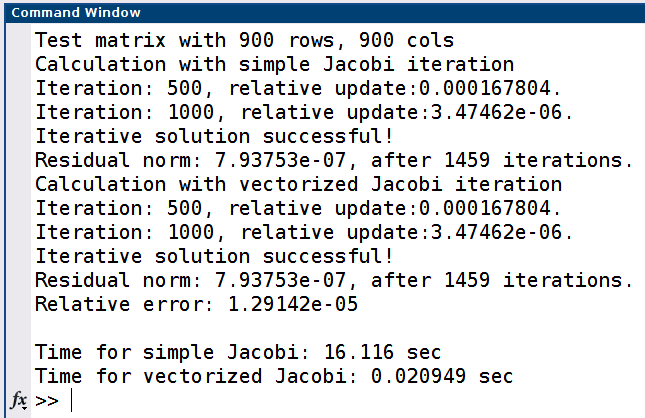
\includegraphics{jacobi-performance-comparison.png}
\caption{Jacobi method performance comparison for $900 \times 900$ test matrix.}
\label{fig:jacobi-performance}
\end{marginfigure}

The main disadvantage of the Jacobi method is \emph{slow convergence}; compared to other methods, it typically takes many iterations to achieve a solution within a specified error tolerance.

\section{MATLAB Implementation of Jacobi Method}
In this section we will present a full implementation of the Jacobi method.

As usual, we start by clearing out the workspace memory and command window output and close any figures.  We use a \lstinline[style=myMatlab]{switch...case} construct to allow selection between different linear systems.

\setcounter{lstannotation}{0}

\marginnote[2.5cm]{
\ref{lst:ann11n-1} A diagonally dominant test matrix.

\vspace{0.25cm}

\noindent \ref{lst:ann11n-2} We customarily use a zero vector for $x^{(0)}$.  In more complex schemes a simple alternative method is used to obtain a low-order approximation of the solution that can thus be used for $x^{(0)}$.  This, unsurprisingly results in faster convergence than the naive choice used here.

\vspace{0.25cm}

\noindent \ref{lst:ann11n-3} Here we use \lstinline[style=myMatlab]{show_x} as a flag to indicate whether or not we want to show the answer in the command window. If I set \lstinline[style=myMatlab]{show_x=1}, that indicates I want the solution, $x$, to be output to the MATLAB command window.  If \lstinline[style=myMatlab]{show_x=0} then $x$ is not output.  If $x$ is a vector with only a few elements, it is worthwhile to visually inspect the result and see that it is correct.  If $x$ has hundreds or thousands of elements, such exercises are useless.


\vspace{0.1cm}  

\noindent \ref{lst:ann11n-4} This is a $900 \times 900$ symmetric, positive definite matrix that has \emph{weak} diagonal dominance.  Weak diagonal dominance relaxes the requirement that the magnitude of the diagonal entry be greater than the sum of the absolute values of the off-diagonal entries; it can also be \emph{equal} to the sum of the off-diagonal elements.
}
\begin{lstlisting}[name=lec11n_jacobi, style=myMatlab]
%% Example: Jacobi Method Demonstration
clear
clc
close 'all'

sys_choice = 2;

switch sys_choice
    
    case 1
        A = [9 -2 3 2;
            2 8 -2 3;
            -3 2 11 -4;   /*!\annotation{lst:ann11n-1}!*/
            -2 3 2 10];
        b = [54.5;
            -14;
            12.5;
            -21];
        rows = 4; cols = 4;
        x_in = zeros(cols,1); /*!\annotation{lst:ann11n-2}!*/
        show_x = 1; /*!\annotation{lst:ann11n-3}!*/
           
    case 2
        [A,rows,cols,entries] = mmread('gr_30_30.mtx'); /*!\annotation{lst:ann11n-4}!*/
        fprintf('Test matrix with %d rows, %d cols \n',...
            rows,cols);
        b = rand(cols,1);
        x_in = zeros(rows,1);
        figure
        spy(A)
        title('Sparsity Pattern of Test Matrix')
        show_x = 0;

    otherwise
        error('Invalid system choice!\n');
end
\end{lstlisting}

We need to specify stopping criteria.  For iterative methods such as those under consideration in this lecture, one possible stopping criteria is shown in Equation \ref{eq:lec11n-iter-converge}.
\begin{equation}
\text{Estimated Relative Error} = \frac{|| x^{(k+1)} - x^{(k)}||_{\infty}}{||x^{(k)}||_{\infty}}
\label{eq:lec11n-iter-converge}
\end{equation}
This stopping criteria has the disadvantage that it does not provide any real assurance that $x^{(k+1)}$ is close to $x^{\star}$.  It only says that $x^{(k+1)}$ is close to $x^{(k)}$.  When evaluating the solution, you should also verify that the residual is small.\sidenote[][-2.0cm]{You might ask: why not just use the relative residual, $\sfrac{||Ax^{(k+1)} - b||}{||b||}$, as a stopping criteria?  My wan answer is: a lot of people use estimated relative error instead.  A somewhat better reason is that if the estimated relative error from Equation \ref{eq:lec11n-iter-converge} is very small, then $x^{(k)}$ is changing only slightly with more iterations and, if the answer is bad at that point, it probably will not get better any time soon.  My only advice is that you should check the relative residual when you are done to make sure your iteration did not converge to a garbage solution.}

The code listing below sets stopping criteria, invokes the Jacobi solver, and evaluates performance.
\marginnote[0.0cm]{

\noindent \ref{lst:ann11n-5} The MATLAB functions \lstinline[style=myMatlab]{tic} and \lstinline[style=myMatlab]{toc} act as a simple timing tool.  The call to \lstinline[style=myMatlab]{tic} starts the clock; when we call \lstinline[style=myMatlab]{toc} the clock is stopped and the elapsed time (in seconds) is returned and, in this case, assigned to the variable \lstinline[style=myMatlab]{time_jac}.

\vspace{0.1cm}

\noindent \ref{lst:ann11n-6} Here we make use of the \lstinline[style=myMatlab]{exit_code} returned from our function.  If \lstinline[style=myMatlab]{exit_code=1}, that means the iterative solver stopped based on the estimated relative error.  

\vspace{1.0cm}

\noindent \ref{lst:ann11n-7} Here we make use of the \lstinline[style=myMatlab]{show_x} variable.  In this context, if \lstinline[style=myMatlab]{show_x} is \emph{not} equal to zero, the Boolean expression \lstinline[style=myMatlab]{if show_x} evaluates as true and the \lstinline[style=myMatlab]{if...end} block is executed; in this case, displaying \lstinline[style=myMatlab]{x} to the MATLAB command window.

}
\begin{lstlisting}[style=myMatlab, name=lec11n_jacobi]
%% Solve using Jacobi Iteration

% set stopping criteria
imax = 1500; % max iterations
tol = 1e-7; % estimated relative error tolerance

fprintf('Calculation with simple Jacobi iteration \n');
tic;
[x_jac,norm_res,num_iter,exit_code] = ...  /*!\annotation{lst:ann11n-5}!*/
    jacobi_solver(A,b,x_in,tol,imax);
time_jac = toc;

if exit_code == 1  /*!\annotation{lst:ann11n-6}!*/
    fprintf('Iterative solution converged!\n');
    fprintf('Residual norm: %g, after %d iterations.\n',...
        norm_res,num_iter);
end

if show_x
   fprintf('x = \n'); disp(x_jac);  /*!\annotation{lst:ann11n-7}!*/
end

fprintf('Calculation with vectorized Jacobi iteration \n');
tic;
[x_jac_v,norm_res_v,num_iter_v,exit_code_v] = ...
    jacobi_solver_v(A,b,x_in,tol,imax);
time_jacv = toc;

if exit_code_v == 1
    fprintf('Iterative solution converged!\n');
    fprintf('Residual norm: %g, after %d iterations.\n',...
        norm_res_v,num_iter_v);
end

if show_x
   fprintf('x = \n'); disp(x_jac_v); 
end

\end{lstlisting}
As previously discussed, even if the iterative scheme converges, we should check the relative residual to see if we have converged to something like the correct solution.  Code to do this is in the next listing.
\marginnote[1.0cm]{
\ref{lst:ann11n-8} The relative residual calculation is implemented as part of the iterative schemes.  It is not used as a stopping criterion but is passed back as a return argument.
}
\begin{lstlisting}[style=myMatlab, name=lec11n_jacobi]
%% Check Relative Residual

fprintf('Relative residual Jacobi: %g \n',norm_res); /*!\annotation{lst:ann11n-8}!*/
fprintf('Relative residual vectorized Jacobi: %g \n',...
    norm_res_v);
\end{lstlisting}

Finally we present the full implementation of the Jacobi iteration.  The basic version is in the listing below:
\begin{lstlisting}[style=myMatlab, name=lec11n-jacobi]
%% Local functions
function [x_new,norm_res,num_iter,exit_code] = ...
    jacobi_solver(A,b,x_in,tol,imax)
[n,~] = size(A);
rel_update = inf;
x_new = x_in; % initialize x_new
for iter = 1:imax
    if (iter > 1) && (mod(iter,500) == 0)
        fprintf('Iteration: %d, relative update:%g. \n',...
            iter,rel_update);
    end 
    for i = 1:n
        x_new(i) = (1/A(i,i))*(b(i) - ...
            A(i,1:(i-1))*x_in(1:(i-1)) - ...
            A(i,(i+1):n)*x_in((i+1):n));
    end
    if norm(x_in,"inf") ~= 0 % prevent nan
        rel_update = ...
            norm(x_new - x_in,"inf")/norm(x_in,"inf");
    end    
    % check exit criteria
    if rel_update < tol
        exit_code = 1; % success
        break; % "break out" of the for loop
    end    
    if iter == imax
        % maximum iterations reached
        exit_code = 0; 
    end
    x_in = x_new;    
end
norm_res = norm(A*x_new - b,2)/norm(x_new,2);
num_iter = iter;
end
\end{lstlisting}
And the, slightly different, vectorized version:

\begin{lstlisting}[style=myMatlab, name=lec11n-jacobi]
function [x_new,norm_res,num_iter,exit_code] = ...
    jacobi_solver_v(A,b,x_in,tol,imax)
rel_update = inf;
x_new = x_in; % initialize x_new
K = -(A - diag(diag(A)));
M_inv = sparse(diag(1./diag(A)));

for iter = 1:imax
    if (iter > 1) && (mod(iter,500) == 0)
        fprintf('Iteration: %d, relative update:%g. \n',...
            iter,rel_update);
    end
    
    x_new = M_inv*(K*x_in + b);

    if norm(x_in,"inf") ~= 0 % prevent nan
        rel_update = ...
            norm(x_new - x_in,"inf")/norm(x_in,"inf");
    end    
    % check exit criteria
    if rel_update < tol
        exit_code = 1; % success
        break; % "break out" of the for loop
    end    
    if iter == imax
        % maximum iterations reached
        exit_code = 0; 
    end
    x_in = x_new;
    
end
norm_res = norm(A*x_new - b,2)/norm(x_new,2);
num_iter = iter;
end
\end{lstlisting}

\subsection{Gauss-Seidel Method}
The Gauss-Seidel method is a minor modification of the Jacobi method.  Recall the basic update scheme for the Jacobi iteration:
\begin{equation*}
x_i^{(k+1)} = \frac{1}{a_{ii}}\left[b_{i} - \sum\limits_{j=1}^{i-1}a_{ij}x_{j}^{(k)} - \sum\limits_{j=i+1}^{n}a_{ij}x_j^{(k)} \right]
%\label{eq:lec11n-Jacobi}
\end{equation*}
and notice that, when we are computing the update for $x_i^{(k+1)}$, if we are indeed carrying out these calculations sequentially for increasing values of $i$, we already have updated values of $x^{(k+1)}_j$ on-hand for $1 \le j < i$.  Why not use them?  Answer: there is no reason why not; let us use them.  The update scheme for Gauss Seidel is given in Equation \ref{eq:lec11n-GS}.
\begin{equation}
x_i^{(k+1)} = \frac{1}{a_{ii}}\left[b_{i} - \sum\limits_{j=1}^{i-1}a_{ij}x_{j}^{(k+1)} - \sum\limits_{j=i+1}^{n}a_{ij}x_j^{(k)} \right]
\label{eq:lec11n-GS}
\end{equation}
The good news is that use of updated values in this way results in the Gauss-Seidel method converging in roughly half as many iterations as the Jacobi method.  The bad news is that the order in which we calculate $x_{i}^{(k+1)}$ matters; we cannot do them in parallel like we could with the Jacobi method.\sidenote{And, perhaps it does not need to be mentioned, given that the vectorized Jacobi method is hundreds of times faster than the non-vectorized version, one may be hard-pressed to give up such an advantage.}  Still, the performance improvement from the vectorized implementation of Jacobi was \emph{heavily} dependent on the fact that we are working in a MATLAB environment.  It would be quite difficult to replicate an equivalent implementation if you were using, for example, C++ or FORTRAN.  So, if you \emph{could not} make use of the inherent parallelism of the Jacobi method, Gauss-Seidel would offer you a significant performance benefit.  

\subsection{Method of Successive Over-Relaxation}
If using updated values of $x^{(k+1)}$ as we do in Gauss-Seidel provides some convergence benefit, maybe we could get more benefit if we used \emph{more} of the updated value.  The method of successive over-relaxation (SOR) does this as shown in Equation \ref{eq:lec11n-sor}:
\begin{equation}
x_{i}^{(k+1)} = (1-\omega) x_{i}^{(k)} + \frac{\omega}{a_{ii}}\left[b_{i} - \sum\limits_{j=1}^{i-1}a_{ij}x_{j}^{(k+1)} - \sum\limits_{j=i+1}^{n}a_{ij}x_j^{(k)} \right]
\label{eq:lec11n-sor}
\end{equation}
where $\omega$ is called a \emph{relaxation parameter}.  It can be shown that, in order to converge, $0 < \omega < 2$; if $\omega<1$, the iteration is referred to as \emph{under-relaxation}; if $1 < \omega < 2$, the iteration is referred as \emph{over-relaxation}.\sidenote{If $\omega = 1$, then SOR is equivalent to Guass-Seidel.}  The convergence benefits obtained through SOR is heavily dependent upon properties of the matrix $A$ of the linear system you are trying to solve.  Readers are encouraged to work through the exercises in the next assignment to get some hands-on experience with this behavior.  

\chapter{Assignment \#4}
\label{ch:ass4n}

\begin{fullwidth}
\begin{enumerate}
\item Determine the LU decomposition of the matrix below by hand.
\begin{equation*}
A = 
\bracketMatrixstack{
2 & 4 & 6 \\
3 & 5 & 1 \\
6 & -2 & 2 
}
\end{equation*}

\vspace{4.0cm}

\item Carry out (by hand) the first three iterations of the solution of the following system of equations using the Gauss-Seidel iterative method.  For the first guess of the solution, take the value of all unknowns to be zero.
\begin{align*}
8x_1 + 2x_2 + 3x_3 &= 51 \\
2 x_1 + 5x_2 + x_3 &= 23 \\
-3x_1 + x_2 + 6x_3 &= 20
\end{align*} 


\vspace{4.0cm}

\item Consider the linear system given below:
\begin{equation*}
\bracketMatrixstack{
4 & 0 & 1 & 0 & 1 \\
2 & 5 & -1 & 1 & 0 \\
1 & 0 & 3 & -1 & 0 \\
0 & 1 & 0 & 4 & -2 \\
1 & 0 & -1 & 0 & 5
}
\bracketVectorstack{
x_1 \\
x_2 \\
x_3 \\
x_4 \\
x_5
}
=
\bracketVectorstack{
32 \\
19 \\
14 \\
-2 \\
41
}
\end{equation*}

\begin{enumerate}
\item Find the solution using the built-in MATLAB function \lstinline[style=myMatlab]{[L,U,P] = lu(A)}---be sure to get and use the permutation matrix \lstinline[style=myMatlab]{P}.
\item Find the relative residual for your solution.
\item Find the inverse of the matrix, $A^{-1}$, using the built-in MATLAB function \lstinline[style=myMatlab]{inv(A)}, and compute the 2-norm of $A$ and $A^{-1}$ using the built-in MATLAB function \lstinline[style=myMatlab]{norm(A,p)}, where \lstinline[style=myMatlab]{p} should be set to 2 for the 2-norm.

\item Calculate the size of the error bound:
\begin{equation*}
\frac{1}{\kappa(A)}\frac{||r||}{||b||} \le \frac{||e||}{||x^{\star}||} \le \kappa(A) \frac{||r||}{||b||}
\end{equation*}
where $\kappa(A)$ is the condition number of $A$, and $r$ is the residual.

\item Repeat steps a) through d) for the test matrix BCSSTK26 from the Matrix Market.  Once you have read the matrix into MATLAB, convert the matrix to a ``full'' (non-sparse) format using the MATLAB built-in function \lstinline[style=myMatlab]{A_full = full(A_sparse)}.  or the right-hand-side vector $b$, use a vector of all ones.  Note how different the error bound is in this case.

\end{enumerate}

\vspace{8.0cm}

\item Using Jacobi, Gauss-Seidel, and SOR $(\omega = 1.4)$ iterative methods, write and run code to solve the following linear system of equations:
\begin{equation*}
\bracketMatrixstack{
7 & 3 & -1 & 2 \\
3 & 8 & 1 & -4 \\
-1 & 1 & 4 & -1 \\
2 & -4 & -1 & 6
}
\bracketVectorstack{
x_1 \\
x_2 \\
x_3 \\
x_4
}
=
\bracketVectorstack{
-1 \\
0 \\
-3 \\
1
}
\end{equation*}
The stopping criterion should be the relative change of the estimated solution in the 2-norm:
\begin{equation*}
\text{tolerance} = \frac{||x^{(k+1)} - x^{(k)}||_2}{||x^{(k)}||_2}
\end{equation*}
with tolerance set to $10^{-9}$.  Compare the number of iterations required in each case.


\vspace{3.0cm}

\item For this problem we will compare two iterative methods to solve BCSSTK26---a test matrix derived from a seismic simulation of a nuclear power plant structure.  For the right-hand-side vector $b$, use a vector of all ones.

\begin{enumerate}
\item Use the SOR method with an estimated relative error tolerance of $10^{-3}$.  Vary the relaxation parameter over the range $\omega \in [1.25,2.0)$.  Make a plot of the number of iterations required as a function of $\omega$ and approximate the best value of $\omega$ for this system.

\item Use the MATLAB built-in function \lstinline[style=myMatlab]{gmres} without a preconditioner to solve this problem.  

\item Use \lstinline[style=myMatlab]{gmres} again but with an incomplete LU preconditioner.  Use \lstinline[style=myMatlab]{opts_ilu.type='ilutp'} and \lstinline[style=myMatlab]{opts_ilu.droptol=dtol} and vary the value of \lstinline[style=myMatlab]{dtol} over the range $\text{dtol} \in [10^{-7},10^{-3}]$.  What happens as \lstinline[style=myMatlab]{dtol} gets larger? \emph{\textbf{Hint:} Use the built-in function \lstinline[style=myMatlab]{spy(L)} to show the sparsity pattern of \lstinline[style=myMatlab]{L} and note the number of non-zeros of \lstinline[style=myMatlab]{L}.  How does \lstinline[style=myMatlab]{nna(L)} change as \lstinline[style=myMatlab]{dtol} is changed?}

\item This is a relatively small sparse system and can be solved using direct methods.  Use the MATLAB built-in function \lstinline[style=myMatlab]{timeit} to estimate the time required to solve the system of equations using the built-in \lstinline[style=myMatlab]{mldivide()}---``backslash''---function.
\end{enumerate}
Organize your findings from part a), b) and c) into a short written document.  A couple of paragraphs should be sufficient.  Include the plot you created from part a) and any other graphics/tables that you find helpful to communicate what you observed in parts b) through d).

\end{enumerate}

\end{fullwidth}

\chapter{Lecture 12 Preconditioning and MATLAB Built-in Methods}
\label{ch:lec12n}
\section{Objectives}
The objectives of this lecture are to:
\begin{itemize}
\item Further discuss required conditions for convergence of iterative methods based on matrix splitting.
\item Discuss preconditioning and its importance for iterative solution methods.
\item Describe MATLAB built-in methods for solving sparse systems of equations using iterative methods.
\end{itemize}
\setcounter{lstannotation}{0}

\section{Conditions for Convergence}
In the last lecture we discussed three iterative methods based on a matrix splitting: $A = M-K$ where $M$ is non-singular and relatively easy to compute.  We used this splitting to try and find solutions to a linear system of equations: $Ax = b$ in an iterative fashion:
\begin{equation*}
x^{(k+1)} = \underbrace{M^{-1}K}_{R}x^{(k)} + \underbrace{M^{-1}b}_{c}
\end{equation*}
were $x^{(0)}$ is an initial guess.

It will probably not come as a surprise to learn that we cannot hope to do this successfully for just any matrix $A$, resulting $R$, or initial guess $x^{(0)}$.

In the last lecture we learned that if a matrix is strictly row diagonally dominant:
\begin{equation*}
|a_{ii}| > \sum\limits_{j \ne i} |a_{ij}|
\end{equation*}
then Jacobi and Gauss Seidel would converge.  This was presented as a \emph{sufficient} condition for convergence---i.e. if true, the method would converge; if not true, the method \emph{might} converge.  A more rigorous convergence criterion is based on the spectral radius of $R = M^{-1}K$.\cite{demmel1997applied}

\index{spectral radius}
\begin{definition}[Spectral Radius]
The \emph{spectral radius} of $R$ is $\rho(R) = \max{|\lambda|}$, where the maximum is taken over all the eigenvalues, $\lambda$, of $R$.
\end{definition} 

\begin{theorem}[Convergence of Splitting-Based Iterative Method]
The iteration $x^{(k+1)} = Rx^{(k)} + c$ converges to the solution of $Ax=b$ for all starting vectors $x^{(0)}$ and for all $b$ if and only if $\rho(R)<1$.
\end{theorem}
It can further be shown that the \emph{rate of convergence}, $r(R)$, giving the increase in the number of correct decimal places in the solution per iteration, can be given by:
\begin{equation}
r(R) = -\log_{10}\rho(R)
\end{equation}

To quickly summarize the results of this section:
\begin{enumerate}
\item For a given splitting-based iterative method, like the Jacobi method, convergence is only assured if: $\rho(R)< 1$; and
\item convergence will require fewer iterations the smaller $\rho(R)$ is.
\end{enumerate}

This begs the question: is there anything we can do if $\rho(R)\ge 1$?  For less dire conditions: if $\rho(R)$ is less than 1 but the rate of convergence is maddeningly slow, is there anything we can do about it?  The answer to both questions is: \emph{yes}, and we describe how in the next section.

\section{Preconditioning}
The basic idea of preconditioning is to transform $A$ so that $\rho(R)$ is made smaller.  For any non-singular $n \times n$ matrix $P$, the systems below have the same solution:
\begin{align*}
Ax &= b \\
P^{-1}Ax &= P^{-1}b
\end{align*}
And so we ask: what choices of $P$ would make $\rho(R)$ smaller?  As an extreme choice, set $P$ = $A^{-1}$; then by definition: $P^{-1}A = I$.  If this is the case, our matrix splitting is: $P^{-1}A = I = M - K$, where $M=I$, $M^{-1}=I$ and $K=0$.  The corresponding iteration would be:
\begin{align*}
x^{(k+1)} &= Rx^{(k)} + c \\
&= M^{-1}Kx^{(k)} + M^{-1}Pb \\
&= \underbrace{I[0]}_{R = 0}x^{(k)} + \underbrace{IA^{-1}b}_{A^{-1}b = x}
\end{align*}
The spectral radius of $R$ is zero and we converge in one step for any choice of $x^{(0)}$.

Obviously this is not a practical method; if we knew what $A^{-1}$ was, we would not be playing with an iterative method.  A more practical approach is to find a $P$ that is \emph{nearly} equal to $A^{-1}$ but easier to compute and store.  When working in a MATLAB environment, our main choice for preconditioner will be the \emph{incomplete LU factorization} given by the built-in function \lstinline[style=myMatlab]{ilu(A,options)}.  

As the name suggests, the incomplete LU factorization creates an approximate LU factorization of sparse matrix $A$.  Recall that the reason why we avoid such factorization for sparse matrices is that it results in undesired ``fill-in'' of the non-zero elements of $A$.  But suppose we carried out the LU factorization but only allowed non-zeros in locations where $A$ is non-zero.  In this case, $A \ne LU$ but $U^{-1}L^{-1} \approx A^{-1}$ and this can serve as a basis for an iterative method.

\subsection{LU and Incomplete LU Preconditioning in MATLAB}
To demonstrate preconditioning, we will use a test matrix obtained from the Matrix Market---\emph{BCSSTK15}---which is a real, symmetric, positive definite matrix based on the structural analysis of an off-shore oil platform.\sidenote[][-5.5cm]{This matrix can be obtained at \url{https://math.nist.gov/MatrixMarket/data/Harwell-Boeing/bcsstruc2/bcsstk15.html}.}  The sparsity pattern is shown in Figure \ref{fig:lec12n-test-matrix-sparsity}.
\begin{marginfigure}[-4.0cm]
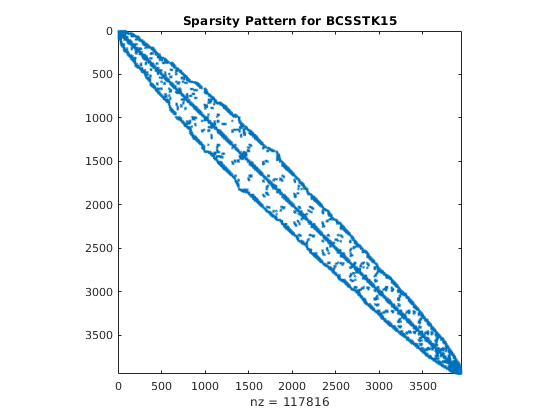
\includegraphics{lec12n-test-matrix-sparsity.png}
\caption{Sparsity pattern for BCSSTK15.}
\label{fig:lec12n-test-matrix-sparsity}
\end{marginfigure}
This matrix is not diagonally dominant\sidenote{You can visit the URL on the Matrix Market for BCSSTK15 to see a variety of matrix properties; diagonal dominance is one such property.  You can, of course, alternatively write your own function to determine whether or not a matrix is diagonally dominant.} so we might want to check the spectral radius to determine if the Jacobi method might succeed.  MATLAB code to determine spectral radius is provided in the listing below:\marginnote{
\ref{lst:ann12n-1}  The built-in function \lstinline[style=myMatlab]{eigs(A,k)} returns the $k$-largest eigenvalues of input (sparse) matrix $A$.  
}
\begin{lstlisting}[style=myMatlab]
K = -(A - diag(diag(A)));
M_inv = sparse(diag(1./diag(A)));

rho = abs(eigs(M_inv*K,1)); /*!\annotation{lst:ann12n-1}!*/
fprintf('Spectral radius of R: %g \n',rho);
\end{lstlisting}
For BCSSTK15, $\rho(A) \approx 3.17$, so we expect the un-preconditioned Jacobi method to fail---and, indeed, it does.  

Suppose we take an extreme approach and use the complete LU factorization as a preconditioner.  \marginnote[1.75cm]{
\ref{lst:ann12n-2} \lstinline[style=myMatlab]{U\\(L\\A)} is equivalent to $U^{-1}L^{-1}A$ and \lstinline[style=myMatlab]{U\\(L\\b)} is equivalent to $U^{-1}L^{-1}b$.  Recall, if $A=LU$, $A^{-1}=U^{-1}L^{-1}$.
}
\begin{lstlisting}[style=myMatlab]
[L,U] = lu(A);
nnzL = nnz(L); nnzU = nnz(U);

PA = U\(L\A); Pb = U\(L\b); /*!\annotation{lst:ann12n-2}!*/

[x_jac2,norm_res2,num_iter2,exit_code2] = ...
    jacobi_solver(PA,Pb,x_in,tol,imax);
if exit_code2 == 1
   fprintf('Preconditioned Jacobi solution successful! \n');
   fprintf('Number of iterations: %d \n',num_iter2);
   fprintf('tol = %g \n',norm_res2);
end
\end{lstlisting}
The output is shown in Figure \ref{fig:lec12n-ex1-lu-precon-out}.  Note the spectral radius of $R$ is near zero and we converged to the solution right away.\sidenote{The only reason 2 iterations were used is because the stopping criterion was based on $|x^{(k+1)}-x^{(k)}|$ and $x^{(0)}$ was far from the solution.}
\begin{marginfigure}
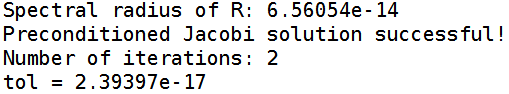
\includegraphics{lec12n-ex1-lu-precon-out.png}
\caption{Output for preconditioning with \emph{complete} LU factorization.}
\label{fig:lec12n-ex1-lu-precon-out}
\end{marginfigure}
The bad news for this example is that, while \lstinline[style=myMatlab]{A} has 117,816 non-zero entries, \lstinline[style=myMatlab]{L} and \lstinline[style=myMatlab]{U} both have on the order of a million non-zeros.  On top of that, we just performed a full LU factorization of $A$ so time spent on Jacobi iterations were wasted.

Let us now, instead us an incomplete LU factorization.\marginnote[0.25cm]{
\ref{lst:ann12n-3} Use these options for \lstinline[style=myMatlab]{ilu(A,options)}. The \lstinline[style=myMatlab]{type='ilutp'} refers to incomplete LU with \emph{threshold} and \emph{pivoting} which improves the reliability of the algorithm.  The \lstinline[style=myMatlab]{droptol} is the \emph{drop tolerance} of the incomplete LU factorization.  The \emph{higher} your value of \lstinline[style=myMatlab]{droptol}, the \emph{more sparse} the resulting \lstinline[style=myMatlab]{L} and \lstinline[style=myMatlab]{U} will be; if \lstinline[style=myMatlab]{droptol} is lower, \lstinline[style=myMatlab]{L} and \lstinline[style=myMatlab]{U} will be less sparse.  In the limit, if \lstinline[style=myMatlab]{droptol=0}, then the complete LU factorization is produced. Setting \lstinline[style=myMatlab]{udiag=1} results in replacing zero diagonal entries of \lstinline[style=myMatlab]{U} with the local drop tolerance.  Selection of this option makes the \lstinline[style=myMatlab]{ilu} algorithm more reliable.  See the MATLAB documentation for \lstinline[style=myMatlab]{ilu} for a more complete description of all available options.
}
\begin{lstlisting}[style=myMatlab]
opts_ilu.type='ilutp';
opts_ilu.droptol=1e-4; /*!\annotation{lst:ann12n-3}!*/
opts_ilu.udiag=1;
[iL,iU] = ilu(A,opts_ilu);
nnz_iL = nnz(iL); nnz_iU = nnz(iU);

iPA = iU\(iL\A); iPb = iU\(iL\b);/*!\annotation{lst:ann12n-4}!*/

[x_jac3,norm_res3,num_iter3,exit_code3] = ...
    jacobi_solver(iPA,iPb,x_in,tol,imax);
if exit_code3 == 1
   fprintf('Preconditioned Jacobi solution successful! \n');
   fprintf('Number of iterations: %d \n',num_iter3);
   fprintf('tol = %g \n',norm_res3);
end
\end{lstlisting}

\vspace{0.25cm}

\noindent \ref{lst:ann12n-4} This is done for illustration purposes only.  Even if \lstinline[style=myMatlab]{iL} and \lstinline[style=myMatlab]{iU} are sparse with a low number of non-zeros, \lstinline[style=myMatlab]{iPA} and \lstinline[style=myMatlab]{iPb} will be full.  Built-in methods can use \lstinline[style=myMatlab]{iL} and \lstinline[style=myMatlab]{iU} without sparsity-destroying operations like this.
The output is shown in Figure \ref{fig:lec12n-ex1-ilu-precon-out1}.  In this case, the spectral radius of $R$ is higher but still less than 1 and, as expected, the number of required iterations to satisfy our solution tolerance is also higher.  Unlike as was the case with the complete LU factorization, the output matrices \lstinline[style=myMatlab]{iL} and \lstinline[style=myMatlab]{iU} are much more sparse, with a total number of roughly 600,000 non-zeros.  
\begin{marginfigure}
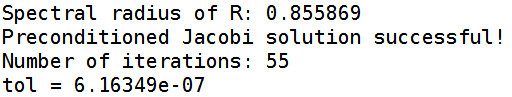
\includegraphics{lec12n-ex1-ilu-precon-out1.png}
\caption{Output for Jacobi iteration with incomplete LU preconditioning.}
\label{fig:lec12n-ex1-ilu-precon-out1}
\end{marginfigure}
If we \emph{increase} the drop tolerance to \lstinline[style=myMatlab]{opts_ilu.droptol=5e-4} we can further reduce the number of non-zeros in \lstinline[style=myMatlab]{iL} and \lstinline[style=myMatlab]{iU} to about 400,000 at the expense of increasing the spectral radius to 0.98 and, as expected, increasing the number of iterations required to reach our stopping criterion to 344.

\section{MATLAB Built-In Iterative Solvers}
There are numerous iterative solvers built into MATLAB.  We will mention only two of them and, sadly, treat them essentially as black-boxes.   
\begin{enumerate}
\item \lstinline[style=myMatlab]{pcg} - preconditioned conjugate gradient method.  
\item \lstinline[style=myMatlab]{gmres} - generalized minimum residuals method.
\end{enumerate}
Both of these algorithms are examples of Krylov subspaces methods, the details of which are beyond the scope of this class. We will use \lstinline[style=myMatlab]{pcg} for linear systems that are symmetric and positive definite.  We will use \lstinline[style=myMatlab]{gmres} for all other methods.  

\subsection{Preconditioned Conjugate Gradient}
The preconditioned conjugate gradient algorithm is one of the most competitive methods for use with sparse, symmetric matrices that are positive definite.  An excellent and easy to read description is available in the open literature.\cite{shewchuk1994conjugate}  Since \lstinline[style=myMatlab]{A} is symmetric, we can use a slightly more efficient algorithm to construct the preconditioning matrix---the incomplete Cholesky factorization: \lstinline[style=myMatlab]{ichol(A,options)}.  An example in its use is shown in the listing below:\marginnote{

\noindent \ref{lst:ann12n-5} See the MATLAB documentation for \lstinline[style=myMatlab]{ichol} for more information on these options.  The option: \lstinline[style=myMatlab]{type='ict'} directs usage of the incomplete Cholesky with threshold dropping.  This option along with \lstinline[style=myMatlab]{droptol} affects the extent to which non-zeros in \lstinline[style=myMatlab]{L} are dropped or retained.  As with \lstinline[style=myMatlab]{ilu()}, \lstinline[style=myMatlab]{droptol=0} results in a full Cholesky factorization.  The option \lstinline[style=myMatlab]{michol='on'} indicates that the modified incomplete Cholesky factorization is to be performed, use of which improves the reliability of the algorithm.
}
\begin{lstlisting}[style=myMatlab]
%% preconditioned conjugate gradient
opts.type = 'ict';
opts.droptol = 1e-4;  /*!\annotation{lst:ann12n-5}!*/
opts.michol = 'on';
L = ichol(A,opts);
[x1,fl1,rr1,it1,rv1] = pcg(A,b,tol,imax,L,L'); /*!\annotation{lst:ann12n-6}!*/

if fl1 == 0
    fprintf('pcg with ichol preconditioner solution successful!\n');
    fprintf('Residual norm: %g, after %d iterations.\n',...
        rr1,it1);
end
\end{lstlisting}

\vspace{0.1cm}

\noindent \ref{lst:ann12n-6} Several of MATLAB's built-in preconditioners use \emph{left} and \emph{right} preconditioners.  As we have described them so far, we have always use a \emph{left} preconditioner.  A right preconditioner works the same way but the matrix is applied to the right:
$$APx = bP  $$
A preconditioning matrix $P$ can be broken up into a left and right preconditioning matrix: $P = P_L P_R^{\prime}$ and applied: $$P_L A P_R^{\prime} x = P_{L}bP_R^{\prime}$$
The last two arguments for \lstinline[style=myMatlab]{pcg} correspond to the left and right preconditioning matrix respectively.   

Readers are encouraged to experiment with the preconditioned conjugate gradient built-in function with different options settings to solve a sparse, symmetric, positive definite, linear system of their choice.

\subsection{Generalized Minimum Residuals}
You should use GMRES for systems that are square and non-singular.  Since the input matrix is not necessarily symmetric or positive definite, you should use \lstinline[style=myMatlab]{ilu} to generate the preconditioning matrices.  An example usage is shown in the listing below.
\begin{lstlisting}[style=myMatlab]
%% GMRES with Incomplete LU Preconditioner
opts_ilu.type='ilutp';
opts_ilu.droptol=1e-3;
restart = [];                /*!\annotation{lst:ann12n-7}!*/
maxit = min(imax,size(A,1));

[L,U] = ilu(A,opts_ilu); 
[x4,fl4,rr4,it4,rv4] = ...
    gmres(A,b,[],tol,maxit,L,U);
\end{lstlisting}
\marginnote[-2.75cm]{

\noindent \ref{lst:ann12n-7} Please see the MATLAB documentation for explanation regarding the arguments to \lstinline[style=myMatlab]{gmres}

}

\chapter{Lecture 13 Least Squares Curve Fitting}
\label{ch:lec13n}
\section{Objectives}
The objectives of this lecture are to:
\begin{itemize}
\item Derive the basic formulas for least squares curve fitting.
\item Do an example using MATLAB.
\end{itemize}
\setcounter{lstannotation}{0}

\section{Introduction}
As an engineer, it is very likely that at some point in time during your career,
you will be called upon to examine and interpret experimental data.  Two
common needs in such analysis are to take a set of experimental data and either:
\begin{enumerate}%[label=\alph*.)]
\item develop a model to represent the data. i.e. find a best fit line (or
  other function) through
  the data; or
\item evaluate the data to determine how well it agrees with some previously
  defined model.  i.e. fit model parameters to the data and assess how well
  the experimentally determined values conform to model expectations.

\end{enumerate}

As an example, we will perform a data-fitting analysis of some wind-tunnel
results as presented in a popular numerical methods textbook.\cite[-1.5cm]{gilat} The behavior that we will explore is the dissipation of vortices shed from the tips and trailing
edges of an airfoil in the wind tunnel.  For this example, the tangential
velocity $\left(V_{\theta}\right)$ of a vortex is measured as it travels down the axis of a
wind-tunnel.  The data are non-dimensionalized by dividing the tangential
velocity of the vortex by the free-stream velocity $\left(V_{\infty}\right)$ and by dividing the vortex
position $\left(R\right)$ relative to the airfoil by the chord-length $\left(C\right)$ of the airfoil.  This non-dimensionalization process will allow experimenters to correlate the results from one particular experiment to larger scale tests on geometrically similar prototypes.  The raw data are given in Table \ref{tab:lec13n-numData} and is shown graphically in Figure \ref{fig:lec13n-theData}.
\begin{marginfigure}[-2.5cm]
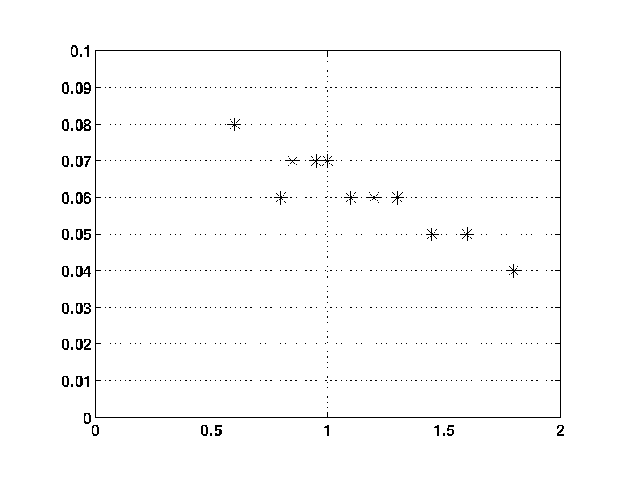
\includegraphics{lec13n_TheData.eps}
\caption{Experimental data from wind tunnel testing.  The $y$-axis is the
  ratio of the tangential velocity of a vortex to the free stream flow
  velocity $\left( y = \sfrac{V_{\theta}}{V_{\infty}}\right)$.  The $x$-axis is
  the ratio of the distance from the vortex core to the chord of an aircraft
  wing. $\left(x = \sfrac{R}{C}\right)$.}
\label{fig:lec13n-theData}
\end{marginfigure}
\begin{table}[h]
\centering
\begin{tabular}{|l|*{11}{c}|}
\hline
$x = \sfrac{V_{\theta}}{V_{\infty}}$ & 0.6 & 0.8 & 0.85 & 0.95 & 1.0 & 1.1 &
  1.2 & 1.3 & 1.45 & 1.6 & 1.8 \\
\hline
$y = \sfrac{R}{C}$ & 0.08 & 0.06 & 0.07 & 0.07 & 0.07 & 0.06 & 0.06 & 0.06 & 0.05 &
  0.05 & 0.04 \\
\hline
\end{tabular}
\caption[][1.5cm]{Numerical data from wind-tunnel experiment.}
\label{tab:lec13n-numData}
\end{table}
In the following sections, we will explore ways in which curves can be fit through this data which, in some sense, are the ``best''-fit curves.

\section{``Guessed''-fit Curves}
It is entirely reasonable, and completely in accord with time honored engineering tradition, to take experimental data as presented in the previous section, use careful judgment and intuition and draw a line that seems to fit the data reasonably well. We will call this the \emph{Guessed}-fit curve and an example of this is shown in Figure \ref{fig:lec13n-guessedfit}.

\begin{marginfigure}
\includegraphics{GuessedFit.eps}
\caption{\emph{Guessed}-fit linear estimation of the experimental data.  $M =
  -0.033$ is the measured slope of the estimated line and $b = 0.1$ is the $y$-intercept.}
\label{fig:lec13n-guessedfit}
\end{marginfigure}  

From this carefully drawn line we may conclude that experimental results show a linear
relationship between tangential velocity and distance downstream from the
airfoil.  Obviously, this model is not perfect; most data-points are off the
line.  Still, we may reasonably decide that overall, this is not a bad
representation of what the data are telling us and leave well enough alone.

\section{Measure of Fitness}

A hand-drawn curve may be well enough for rough analysis, but for the purposes of this lecture, let us assume that we would like to know how good our roughly drawn curve is and wonder if there may be a way to do better.  We have a good fit; but how good is it?  In this section we will answer that question.  We will define a \emph{measure of fitness} so that we may quantitatively determine how ``good'' a candidate curve is in representing the data.

 
For this purpose, we define the \emph{residual}.  In words, the residual $(r_i)$ is the
difference, at each experimental data point $(x_i)$, between the $y$-value given from experimental data $(y_i)$ and the $y$-value computed from our linear ``guessed'' fit curve $\left(y_{\text{guessed}}\right)$.  The mathematical expression for this is given in Equation \ref{resid}.

\begin{equation}
r_{i} = y_{i} - \underbrace{\left(b + Mx_{i}\right)}_{y_{\text{guessed}}} \ \ i = 1,2,\dots,n
\label{resid}
\end{equation}
where $b$ is the $y$-intercept of this linear fit and $M$ is the slope of
the linear fit through the data
and $n$ is the number of data points.

With an eye towards a more general approach, we will re-state Equation \ref{resid} using matrix-vector notation in Equation \ref{residV2}.

\begin{equation}
\begin{split}
\mathbf{r} &= \mathbf{y} - \underbrace{\left( b \cdot \mathbf{x}^0 + M \cdot
\mathbf{x}^{1}\right)}_{\mathbf{y}_{\text{guessed}}} \\
 &= \mathbf{y} - 
\left[
\begin{matrix}
\mathbf{x}^{0} & \mathbf{x}^{1}
\end{matrix}
\right]
\left[
\begin{matrix}
b \\
M
\end{matrix}
\right] \\
&= \mathbf{y} - \mathbf{X}\mathbf{c}
\end{split}
\label{residV2}
\end{equation}

To be clear, please note that $x^{k}$ refers to element-wise exponentiation and in particular, $\mathbf{x}^{0}$ means: ``each element of $\mathbf{x}$ raised to the power of zero,'' and $\mathbf{x}^{1}$ means: ``each element of $\mathbf{x}$ raised to the first power.''  

In order to determine how well a given curve fits the data, the residual given in Equation \ref{residV2} is not quite satisfactory; it is a vector, not a number.  The usual solution to this problem is to use the Euclidean length of the residual as shown in Equation \ref{norm2Resid}:

\begin{equation}
\begin{split}
||r|| &= \sqrt{\mathbf{r}^{T} \mathbf{r}} \\
 &= \sqrt{\sum_{i=1}^{n} r_{i} \cdot r_{i}} 
\end{split} 
\label{norm2Resid}
\end{equation}

For historical reasons, we will depart from this convention and use the ``Euclidean length squared,'' or simply the square of the residual.  We show this in Equation \ref{residSquared} where we also explicitly expand $\mathbf{r}$ as defined in Equation \ref{residV2} to show the residual in terms of the given data $\mathbf{y}$, the matrix $\mathbf{X}$ of our fitting curve and parameter vector $\mathbf{c}$.

\begin{equation}
\begin{split}
\mathbf{r}^{2} &= \mathbf{r}^{T} \mathbf{r} \\
 &= \left(\mathbf{y} - \mathbf{X}\mathbf{c}\right)^{T}\left(\mathbf{y} -
\mathbf{X}\mathbf{c}\right) \\
&= \mathbf{y}^{T}\mathbf{y} - 2 \mathbf{c}^{T}\mathbf{X}^{T}\mathbf{y} +
\mathbf{c}^{T}\mathbf{X}^{T}\mathbf{X}\mathbf{c} 
\end{split}
\label{residSquared}
\end{equation}

The error measure given in Equation \ref{residSquared} now is a single
non-negative number that will in general be zero only if the fitted line passes exactly through all data points.  This is the measure of fitness that we will use.
Using the given values of $\mathbf{y}$, $\mathbf{X}$ and $\mathbf{c}$ for the
``guessed''-fit curve, we find that $\left(\mathbf{r_{\text{guessed}}}\right)^{2} = 0.0152.$ 

\section{Method of Least Squares}

So far we have naively attempted to fit the data as best as we can by guessing
a linear function that might in some way represent the data.  We have defined
an error measure that confirms our suspicion that our linear curve fit is not
perfect.  It is natural to wonder: is there a line that \emph{best} fits the
data\sidenote{At least ``best'' by some error measure.  Different error measures sometimes yield different answers as to what constitutes ``the best.''} and if so, how do we find it? The answer is \emph{``yes, there is a way to find the best fit line''} and the method to find it is called the method of least squares. 

\subsection{Algebraic Derivation}

The standard algebraic derivation of the method of least squares starts with the squared residual given in Equation \ref{residSquared}.  As you should take a moment to confirm, once we have selected a linear estimator\sidenote{
i.e. we have chosen what functions will be used to make up the columns of
$\mathbf{X}$---for the time being we decided it would be composed of the 0\textsuperscript{th}
and 1\textsuperscript{st} powers of $\mathbf{x}$} $\mathbf{X}$, the only free parameter in Equation
\ref{residSquared} are the coefficients that make up $\mathbf{c}$.  The goal
is to figure out how to choose $\mathbf{c}$ such that the error given in
Equation \ref{residSquared} is as small as possible.

Recall from your introductory calculus courses that the way to minimize a
function is to take the first and second derivative of the function; solve for
the values of the free parameter $(\mathbf{c})$ so that the first derivative
is equal to zero; and verify that the second derivative is positive.  When the
first derivative is zero, the function is at an extremum; when the second
derivative is positive, that extremum is a minimum.

Carrying out this idea, we will take the derivative of Equation
\ref{residSquared} and set the first derivative equal to zero:

\begin{equation}
\begin{split}
\frac{d}{d\mathbf{c}}\mathbf{r}^{2} = 0  - 2\mathbf{X}^{T}\mathbf{y} + \underbrace{\mathbf{X}^{T}\mathbf{X}\mathbf{c} + \mathbf{c}^{T}\mathbf{X}^{T}\mathbf{X}}_{\mathbf{X}^{T}\mathbf{X}\mathbf{c} = \mathbf{c}^{T}\mathbf{X}^{T}\mathbf{X}} &= 2\left(-\mathbf{X}^{T}\mathbf{y}+
\mathbf{X}^{T}\mathbf{X} \mathbf{c}\right) = 0 \\
&\Rightarrow -\mathbf{X}^{T}\mathbf{y} + \mathbf{X}^{T}\mathbf{X}\mathbf{c} =
0 \\
&\Rightarrow \mathbf{X}^{T}\mathbf{X} \mathbf{c} = \mathbf{X}^{T}\mathbf{y}
\end{split}
\label{normalEq}
\end{equation}

We now have to ask: can we find a unique vector $\mathbf{c}$ such that the
last line in Equation \ref{normalEq} is satisfied?  The answer is:
yes---provided only that the columns of $\mathbf{X}$ are linearly
independent,\sidenote{If the columns of $\mathbf{X}$ are linearly independent, this means---by definition---that $\mathbf{Xy} = 0$ if and only if $\mathbf{y}=0$.} $\mathbf{X}^{T}\mathbf{X}$ will be positive-definite and thus non-singular.\sidenote{When a matrix---$\mathbf{A} =
  \mathbf{X}^{T}\mathbf{X}$--- is positive definite, that means that
  $\mathbf{y}^{T}\mathbf{Ay}=0$ if and only if $\mathbf{y}=0$.  So $\mathbf{y}
  \ne 0$ and if the columns of $\mathbf{X}$ are linearly independent ($\mathbf{Xy} \ne 0$),
  then $\mathbf{y}^{T}\mathbf{X}^{T}\mathbf{X}^{T}\mathbf{y} \ge 0$ and can
  \emph{only} be equal to zero if $\mathbf{y}=0$.  As is discussed in
  in previous lectures, positive-definiteness is a sufficient condition for a solution to Equation
  \ref{normalEq} to exist.}  This means that a unique value of $\mathbf{c}$
will exist and that it will be non-zero:

\begin{equation}
\mathbf{c} = \left(\mathbf{X}^{T}\mathbf{X}\right)^{-1}
\left(\mathbf{X}^{T}\mathbf{y}\right)
\label{lstSqSol}
\end{equation} 


MATLAB code to carry out this process is given below:

\begin{lstlisting}[style=myMatlab]
x = [0.6 0.8 0.85 0.95 1.0 1.1 1.2 1.3 1.45 1.6 1.8]; 
y = [0.08 0.06 0.07 0.07 0.07 0.06 0.06 0.06 0.05 0.05 0.04]; 

X = nan(length(x),2);
X(:,1) = (x').^0;
X(:,2) = (x').^1;

c = (X'*X) \ (X'*y');
\end{lstlisting}

Executing this code with our given data we solve for $\mathbf{c}$ which gives
us the $y$-intercept and slope of a different linear curve for the data which we will tentatively call the ``best'' linear fit. The resulting line is presented along with the previous ``guessed''-fit curve
for comparison in Figure \ref{fig:lec13n-bestFitPlot}.  Using Equation \ref{residSquared}, we find that the squared residual of this solution is: 0.0140 which is slightly better than our previous ``guessed''
estimate of 0.0152.

\begin{marginfigure}
\includegraphics{BestFit.eps}
\caption{Best fit linear estimation of the experimental data.  $M =
  -0.0288$ is the measured slope of the estimated line and $b = 0.0940$ is the $y$-intercept.}
\label{fig:lec13n-bestFitPlot}
\end{marginfigure}  



The second step is to prove that the coefficient array $\mathbf{c}$ really is a minimum and not a maximum or saddle-point.    One answer is to say that if we, once again, take the derivative of Equation \ref{normalEq}, we get:

\begin{equation}
\begin{split}
\frac{d^{2}}{d \mathbf{c}^{2}}\mathbf{r}^{2} &= \frac{d}{d \mathbf{c}} \left(-\mathbf{X}^{T}\mathbf{y} + \mathbf{X}^{T}\mathbf{X}\mathbf{c}\right) \\
&= \mathbf{X}^{T}\mathbf{X}
\end{split}
\label{secondDeriv}
\end{equation}

The problem with this, is that the last line of Equation \ref{secondDeriv} is not simply a number; it is a matrix. It turns out that if the columns of $\mathbf{X}$ are linearly independent, then the square matrix $\mathbf{X}^{T}\mathbf{X}$ is symmetric and positive definite.  The property of a matrix: ``symmetric, positive definite'' carries with it some implications:

\begin{enumerate}
\item all of the eigenvalues of the matrix are real and positive; and
\item the matrix is invertible
\end{enumerate}

Though it may smack of hand-waving, the author requests your indulgence and accept that these properties carry the same implications as a positive second derivative for the residual function.  The curve found via the method of least squares is, in fact, the curve with the minimum residual; not an inflection point and definitely not the maximum.\sidenote{The existence of the ``guessed''-fit curve with a higher residual than the curve found using the method of least squares should be convincing proof that the method of least squares, at least, does not find the curve with the maximum residual.}


Based on the mathematical results of this section we can
assert that no \emph{linear} estimator of this data set can
achieve a squared residual error of less than 0.0140.

\section{Linear Least Squared with Non-Linear Estimator}

So far, we have accomplished much, but what do we do in the case where we do
not expect the $x$ and $y$ data that we collected in our experiment to be
linearly related?  The answer is a straight-forward
extension of the method of least squares presented in the preceding section.  

Suppose we would like to find the best quadratic fit through the data?  That
is, we are seeking some function: $c_{1} + c_{2}\mathbf{x} + c_{3}
\mathbf{x}^{2}$ such that the squared residual is as small as possible.  All
that we need to do is to re-define $\mathbf{c}$ to accommodate the extra
parameter and re-define $\mathbf{X}$ to incorporate the extra functional dependence on $\mathbf{x}$.  Specifically:

\begin{equation}
\begin{split}
\mathbf{c} &= 
\left[
\begin{matrix}
c_{1} & c_{2} & c_{3} 
\end{matrix}
\right]^{T} \\
\mathbf{X} &= 
\left[
\begin{matrix}
\mathbf{x}^{0} & \mathbf{x}^{1} & \mathbf{x}^{2}
\end{matrix}
\right]
\end{split}
\label{bestQuad}
\end{equation}

We use this newly defined $\mathbf{X}$ and solve for the corresponding values
of $\mathbf{c}$ using Equation \ref{lstSqSol} \emph{exactly as before}.(!!) Nothing in the process need change because, just as with the linear estimator, all that is required is that the columns of $\mathbf{X}$ be linearly independent. To highlight how general this concept is, we will again change our notation slightly and write $\mathbf{X}$ as:

\begin{equation}
\mathbf{X} = 
\left[
\begin{matrix}
f_{1}(\mathbf{x}) & f_{2}(\mathbf{x}) & \cdots & f_{k}(\mathbf{x})
\end{matrix}
\right]
\end{equation}  
where here $k$ is the index of the columns of $\mathbf{X}$.  For the linear case, $f_{1}(\mathbf{x}) = 1$, $f_{2}(\mathbf{x}) = \mathbf{x}$.  For the quadratic case, we simply add $f_{3}(\mathbf{x}) = \mathbf{x}^{2}$.  Each of the functions: $f_{1}$, $f_{2}$ and $f_{3}$ are linearly independent.\sidenote{Here again a definition is worthwhile.  For a set of   functions to be linearly independent it implies that for scalar values   $c_{i}$, $c_{1}f_{1}(\mathbf{x}) + \cdots + c_{k}f_{k}(\mathbf{x}) = 0$ if and only if $c_{1} = \cdots = c_{k} = 0$.  All of the monomials: 1, $x$, $x^2$, etc... as easily seen to be linearly independent.} Taking this a step further, we could use \emph{any} set of linearly independent functions and Equation \ref{lstSqSol} would still have a unique solution that would provide the parameter vector $\mathbf{c}$ such that the squared residual will be as small
as possible.

The process of using high order polynomials to fit data is so common, that MATLAB has a built-in function---polyfit---to automate least-squares estimation with polynomial estimators.  The code block below does this for second order, third order and sixth order polynomials.  The resulting estimators are given in Figure \ref{HighOrderFitPlot}.  

\begin{lstlisting}[style=myMatlab]
x = [0.6 0.8 0.85 0.95 1.0 1.1 1.2 1.3 1.45 1.6 1.8]; 
y = [0.08 0.06 0.07 0.07 0.07 0.06 0.06 0.06 0.05 0.05 0.04]; 
cSecond = polyfit(x,y,2); 
ySecond = cSecond(1)*x.^2 + cSecond(2)*x + ...
    cSecond(3);
cThird = polyfit(x,y,3);
yThird = cThird(1)*x.^3 + cThird(2)*x.^2 + ...
    cThird(3)*x + cThird(4);
cSixth = polyfit(x,y,6);
ySixth = cSixth(1)*x.^6 + cSixth(2)*x.^5 + ...
    cSixth(3)*x.^4 + cSixth(4)*x.^3 + cSixth(5)*x.^2 + ...
    cSixth(6)*x + cSixth(7);
\end{lstlisting}


\begin{marginfigure}[-5.5cm]
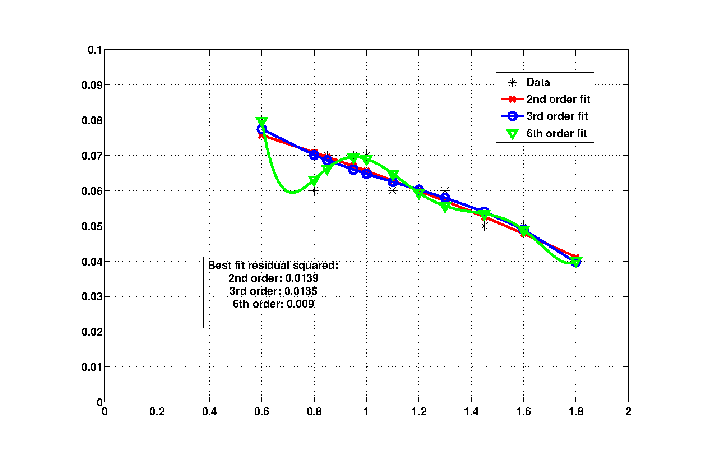
\includegraphics{HigherOrder.eps}
\caption{Best fit linear estimation of the experimental data using 2nd order,
  3rd order and 6th order estimators.}
\label{HighOrderFitPlot}
\end{marginfigure}  

\section{Model Estimators}

As can be seen from Figure \ref{HighOrderFitPlot}, it is possible to find estimators that greatly reduce the squared residual.\sidenote[][-2.5cm]{In general it is possible to find a polynomial that exactly interpolates any number of data points with the resulting residual equal to zero.  It turns out, doing this with polynomial interpolants is usually a very bad idea---at least with ordinary monomials and with equally spaced data points---and when using non-exact floating point arithmetic, and a large number of data points is involved, it is practically impossible.  Better interpolation methods with non-equally-spaced points are almost always used where very accurate interpolation is necessary (for example: when implementing high order finite element methods).}  As higher order estimators are used, the resulting curve through the data becomes problematic.  For example, how would one justify the ``curvy'' nature of the 6th-order approximator?  If we re-performed the experiment with improved instrumentation and made our measurements more carefully, do we \emph{actually} expect the data to follow the 6th order curve?  Probably not.  

It is also worthwhile to consider that the purpose of doing all of this least squares estimation is \emph{not} always to find some curve that comes close to interpolating all of the data.  Rather, the purpose may be to fit the data to a rational scientific model where the experimental data either confirms and strengthens the proposed model for the phenomena under consideration, or serves as the basis for creation of a new model.\cite{trefethen2}

For this example, it turns out that theoretical models do exist regarding the expected vortex velocity as it travels downstream from an airfoil in a wind-tunnel.  This model predicts that the relationship between $y$---the ratio between the vortex tangential velocity and the free-stream velocity---and $x$---the ratio of the distance from the vortex core to the chord of the airfoil section---should have the form of Equation \ref{modelRelation}.

\begin{equation}
y = \frac{A}{x} + \frac{B e^{-2 x^{2}}}{x}
\label{modelRelation}
\end{equation}

As before, we can develop an estimator that conforms with this model in exactly the same way we did for the polynomial estimators.  MATLAB code accomplishing this is provided in the code block below:

\begin{lstlisting}[style=myMatlab]
X = nan(length(x),2);
f1 = @(t) (1./t); % functional form of first term
f2 = @(t) exp(-2*t.^2)./t; % functional form of second term
X(:,1) = f1(x');
X(:,2) = f2(x');
cModel = X\(y');
\end{lstlisting}

Please note a couple of differences between this code and code previously provided:

\begin{enumerate}%[label=\alph*.)]
\item Anonymous functions are used to simplify the construction of
  $\mathbf{X}$.  This is a stylistic choice but could be useful for
  cases where you want to automate this process.
\item The usual ``backslash'' left division operator was used instead of the formula specified in Equation \ref{lstSqSol}.  The reason this works is because
  MATLAB automatically checked and noted that $\mathbf{X}$ was not a square
  matrix (normally a requirement for left matrix division); seeing it was
  not square, then it checked to see if each column of $\mathbf{X}$ is
  linearly independent; MATLAB determined that they were and used the equivalent of
  Equation \ref{lstSqSol} to solve for $\mathbf{c}$.\sidenote[][-4.0cm]{The normal
    equations is the easiest method to derive, but actually solving the normal
    equations directly turns out not to be the very best way of finding
    $\mathbf{c}$.}  
\end{enumerate}

The resulting curve, along with the linear estimator is shown in Figure \ref{modelPlot}.


\begin{marginfigure}[-2.0cm]
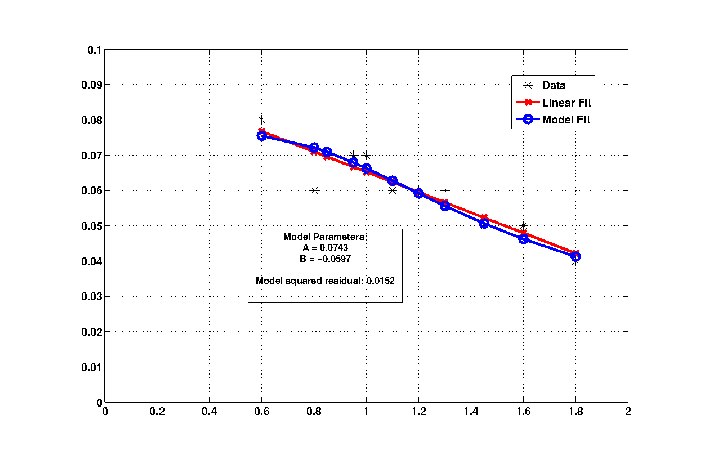
\includegraphics{Model.eps}
\caption{Best fit curve with theoretical model parameters.  The linear Least
  Squares estimator is shown for reference.}
\label{modelPlot}
\end{marginfigure}  


As we can see, the residual squared for the theoretical model estimator is larger than the residual squared for the linear estimator shown previously. Remember, the purpose of fitting a curve through the data points in this context is to gain insight as to how well the recorded experimental data can fit against a known (or proposed) theoretical model.  If we wanted a residual of zero, we could have gotten it through the mechanical process of providing an exact interpolant through the data; but that would hardly yield a reasonable model.  Even though the residual of this new model is higher than for a linear estimator, we gain the benefit of seeing how well the theoretical model stands up in the face of experimental evidence.  

\section{MATLAB Example}

In an electrophoretic fiber-making process, the diameter of the fiber, $d$, is related to the current flow, $I$.  The following measurements are made during production:
\begin{table}[h!]
\begin{tabular}{|l|l|l|l|l|l|l|l|l|l|}
\hline
$I$ (nA) & 300 & 300 & 350 & 400 & 400 & 500 & 500 & 650 & 650 \\ \hline
$d$ ($\mu$m) & 22 & 26 & 27 & 30 & 34 & 33 & 33.5 & 37 & 42 \\ \hline
\end{tabular}
\caption{Process data from electrophoretic fiber-making process.}
\end{table}

\begin{enumerate}
\item Use linear least-squares regression to determine the coefficients $m$ and $b$ in the function $y=mx+b$ that best fits the data.
\item Use least-squares regression to determine the coefficients $a$, $b$, and $c$ in the function $y = a + bx + cx^2$.
\item Use least-squares regression to determine the coefficients $a$ and $b$ in the function $y = a + b\sqrt{I}$.
\end{enumerate}

We start, as always, by clearing out the workspace and command window and closing any open figure windows.  We will also input the given data.
\begin{lstlisting}[style=myMatlab,name=lec13n-ex1]
clear
clc
close 'all'

%% Input Data
I = [300 300 350 400 400 500 500 650 650]';
d = [22 26 27 30 34 33 33.5 37 42]';

\end{lstlisting}

The linear least-squares regression is carried out in the following code; the best fit line is shown in Figure \ref{fig:lec13n-ex1-linear-fit}
\begin{marginfigure}
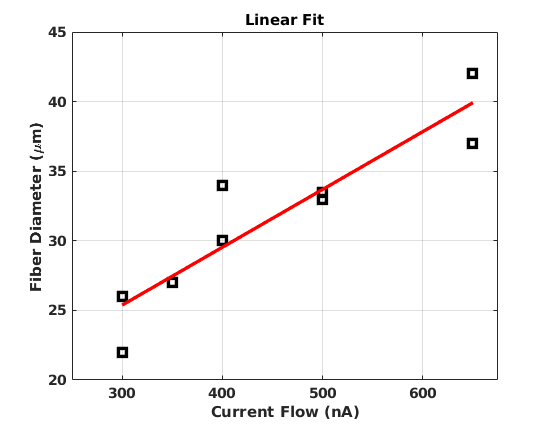
\includegraphics{lec13n-ex1-linear-fit.png}
\caption{Linear fit, $m=0.416$, $b=12.913$.}
\label{fig:lec13n-ex1-linear-fit}
\end{marginfigure}
\begin{lstlisting}[name=lec13n-ex1, style=myMatlab]
X = [ I.^0 I.^1];
b = d;

c = (X'*X)\(X'*b);

linEst = @(x) c(1) + c(2)*x;
\end{lstlisting}
A least-squares regression to fit a second-order polynomial to the data is carried out in the next listing.
\begin{lstlisting}[name=lec13n-ex1,style=myMatlab]
X = [I.^0 I.^1 I.^2];
b = d;

c = (X'*X)\(X'*b);

quadEst = @(x) c(1) + c(2)*x + c(3)*x.^2;
\end{lstlisting}
A plot of the resulting estimator is shown in Figure \ref{fig:lec13n-ex1-second-order-fit}.
\begin{marginfigure}
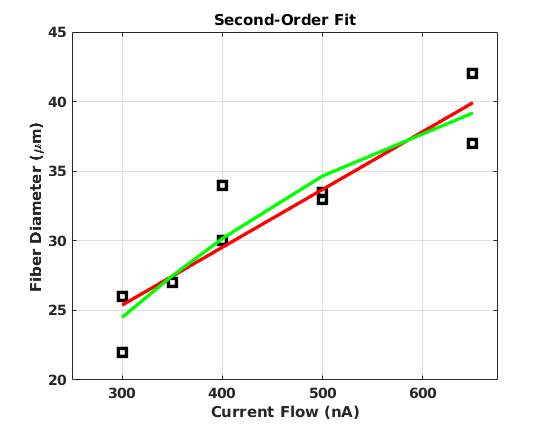
\includegraphics{lec13n-ex1-second-order-fit.png}
\caption{Second-order polynomial fit. $a=0.436$, $b=0.0979$, and $c=-5.89e-5$.}
\label{fig:lec13n-ex1-second-order-fit}  
\end{marginfigure}
Using an estimator like $y = a + b\sqrt{I}$ is accommodated in exactly the same way; there is a constant term---proportional to $I^{0}$---and a term proportional to $I^{\sfrac{1}{2}}$.  The MATLAB code is shown in the listing below and the resulting estimator, along with the previously found estimators, is shown in Figure \ref{fig:lec13n-ex1-model-fit}.

\begin{marginfigure}
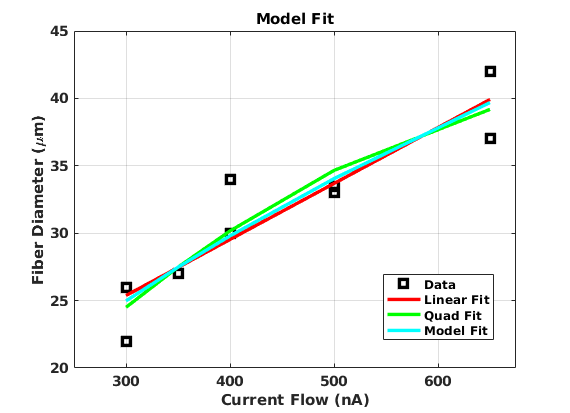
\includegraphics{lec13n-ex1-model-fit.png}
\caption{Model fit of data.  $a = -6.20$, $b=1.80$.} 
\label{fig:lec13n-ex1-model-fit}
\end{marginfigure}

\begin{lstlisting}[style=myMatlab,name=lec13n-ex1]
X = [I.^0 I.^0.5];
b = d;
c = (X'*X)\(X'*b);

est3 = @(x) c(1) + c(2)*x.^0.5;
\end{lstlisting}


\chapter{Lecture 14 Curve Fitting with Non-linear Functions}
\label{ch:lec14n}
\section{Objectives}
The objectives of this lecture are to:
\begin{itemize}
\item Explain how to carry out least squares curve fitting with a nonlinear equation.
\item Do an example using MATLAB.
\end{itemize}
\setcounter{lstannotation}{0}

\section{Curve Fitting with Nonlinear Equation}
The method of least squares requires the estimator to be a linear combination of functions---although, in most cases the individual functions are not linear. If the estimator is non-linear, then you need to linearize it, if possible, through an appropriate transformation.  A variety of useful transforms are presented in Table \ref{transform}.\cite[-2.5cm]{gilat}

\begin{table}[h]
\centering
\begin{tabular}{|p{0.75in}|p{1.55in}|p{1.25in}|p{1.3in}|}
\hline
Nonlinear equation & Linear Form & Relationship to $Y = a_{1}X + a_{0}$ &
Values for linear least-squares regression \\
\hline
$ y = bx^{m}$ & $\ln(y)=m\ln(x)+\ln(b)$ & $Y = \ln(y),\ \  X = \ln(x),
\ \  a_{1} = m, \ \  a_{0} = \ln(b) $ & $\ln(x_{i})$ and $\ln(y_{i})$ \\
\hline
$y = be^{mx}$ & $\ln(y)=mx+\ln(b)$ & $Y = \ln(y), X=x, a_{1}=m, a_{0} = \ln(b)$ &
$x_{i} \text{ and } \ln(y_{i})$ \\
\hline
$y = b10^{mx}$ & $\log(y) = mx + \log(b)$ & $Y = \log(y)$, $X=x$ $a_{1}=m$,
$a_{0} = \log(b)$  & $x_{i}$ and $\log(y_{i})$ \\
\hline
$y = \frac{1}{mx + b}$ & $\frac{1}{y} = mx + b$ & $Y=\frac{1}{y}$, $X=x$,
$a_{1}=m$, $a_{0} = b$ & $x_{i}$ and $\sfrac{1}{y_{i}}$ \\
\hline
$y = \frac{mx}{b + x}$ & $\frac{1}{y} = \frac{b}{m}\frac{1}{x} + \frac{1}{m} $
& $Y=\frac{1}{y}$, $X=\frac{1}{x}$, $a_{1}=\frac{b}{m}$, $a_{0}=\frac{1}{m}$ &
$\sfrac{1}{x_{i}}$ and $\frac{1}{y_{i}}$ \\
\hline
\end{tabular}
\caption[][-1.0cm]{Transforming nonlinear equations to linear form.}
\label{transform}
\end{table}
We will use these transformations in the examples that follow.

\vspace{3.5cm}

\noindent \textbf{Example \#1:} Data are provided in the table below.
\begin{table}
\begin{tabular}{|l|l|l|l|l|l|}
\hline
$x$ & 1 & 2 & 3 & 5 & 8 \\ \hline
$y$ & 0.8 & 1.9 & 2.2 & 3 & 3.5 \\ \hline 
\end{tabular}
\caption{Table of data for Example \#1.}
\label{tab:lec14n-ex1}
\end{table}

\vspace{0.2cm}

\noindent Determine the coefficients $m$ and $b$ in the function $y=\left[m\sqrt{x} + b\right]^{\sfrac{1}{2}}$ that best fits the data.  

\vspace{0.2cm}


\noindent \textbf{Solution: }Here, right off the bat, we have a case that is not represented in Table \ref{transform}.  Nonetheless, we will persevere and notice without too much difficulty that if I make the transformation $p = y^2$, then the estimator for $p$ is given by: $p = m\sqrt{x} + b$.  MATLAB code to load the data and calculate the coefficients of the, now, linearized, estimator is provided below.
\marginnote[1.5cm]{\textbf{Note: } Both of the vectors for $x$ and $y$ are constructed so as to be \emph{column vectors}.  We follow this practice for the other examples as well so that we can employ the same MATLAB equations for carrying out least squares regression and satisfy the semantics of each linear algebraic operation.}
\begin{lstlisting}[style=myMatlab]
clear
clc
close 'all'

% data
x = [1 2 3 5 8]';
y = [0.5 1.9 2.2 3 3.5]';

% linearized estimator
p = y.^2;
X = [x.^0 x.^(0.5)];

C = (X'*X)\(X'*p);

%remember to "undo" the linearizing transformation
est1 = @(x) sqrt(C(1) + C(2)*sqrt(x));
\end{lstlisting}
Notice how we needed to apply the inverse of the linearizing transformation to recover the desired estimator.  Results are shown in Figure \ref{fig:lec14n-ex1}.
\begin{marginfigure}[-4cm]
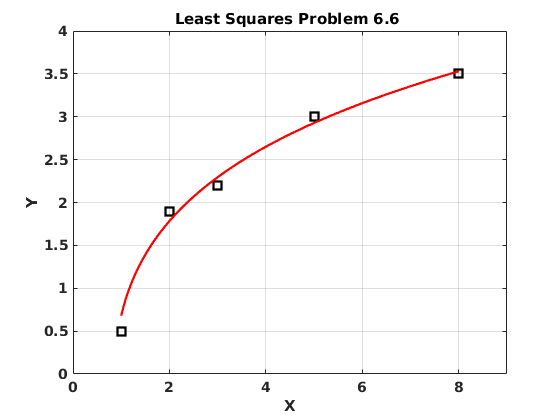
\includegraphics{lec14n-ex1.png}
\caption{Plot of least squares estimator for Example \#1.}
\label{fig:lec14n-ex1}
\end{marginfigure}

\vspace{0.5cm}

\noindent \textbf{Example \#2:} Consider the following given data.

\begin{table}
\begin{tabular}{|l|l|l|l|l|l|}
\hline
$x$ & -2 & -1 & 0 & 1 & 2 \\ \hline
$y$ & 1.5 & 3.2 & 4.5 & 3.4 & 2 \\ \hline 
\end{tabular}
\caption{Table of data for Example \#2.}
\label{tab:lec14n-ex2}
\end{table}

\vspace{0.2cm}

\noindent Determine the coefficients $a$ and $b$ in the function $y=\frac{a}{x^2 + b}$ that best fit the data.

\vspace{0.2cm}


\noindent \textbf{Solution: } The form of this non-linear estimator is similar to that presented in the 4\textsuperscript{th} row of Table \ref{transform}.  
\begin{align*}
p &= \frac{1}{y} \\
&= \frac{x^2 + b}{a} \\
&= \frac{x^2}{a} + \frac{b}{a} \\
&= c_1 x^2 + c_2
\end{align*}
where $c_1 = \sfrac{1}{a}$ and $c_2 = \sfrac{b}{a}$.  We implement the linear least squares in MATLAB in the, by now, familiar style: \marginnote[3.0cm]{

\noindent \ref{lst:ann14n-1} Since $c_1 = \sfrac{1}{a}$, then $a = \sfrac{1}{c_1}$.

\vspace{0.15cm}

\noindent \ref{lst:ann14n-1} Here $c_2 = \frac{b}{a}$ so 
\begin{align*}
c_2 a &= \frac{b}{a} a \\
&= b
\end{align*}
}
\begin{lstlisting}[style=myMatlab]
clear
clc
close 'all'

% data
x = [-2 -1 0 1 2]';
y = [1.5 3.2 4.5 3.4 2]';

% linearized estimator
X = [x.^2 x.^0];
b = y.^(-1);

C = (X'*X)\(X'*b);

% remember to "undo" the linearizing transformation
a = 1./C(1); /*!\annotation{lst:ann14n-1}!*/
b = C(2)*a;  /*!\annotation{lst:ann14n-2}!*/
\end{lstlisting}
A plot of the resulting estimator is shown in Figure \ref{fig:lec14n-ex2}.
\begin{marginfigure}[-0.25cm]
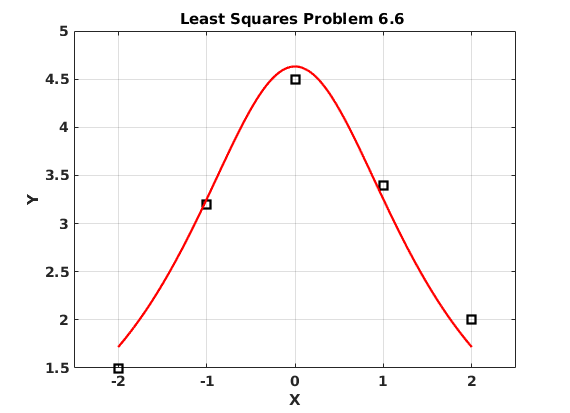
\includegraphics{lec14n-ex2.png}
\caption{Plot of least squares estimator for Example \#2.}
\label{fig:lec14n-ex2}
\end{marginfigure}

\vspace{0.5cm}

\noindent \textbf{Example \#3:} Water solubility in jet fuel, $W_s$, is a function of temperature, $T$, and can be modeled by an exponential function of the form:
\begin{equation*}
W_s = be^{mT}
\end{equation*}
Table \ref{tab:lec14n-ex3} presents measured values of water solubility over a range of temperatures.  
\begin{table}
\begin{tabular}{|l|l|l|l|l|l|}
\hline
$T \ (^{\circ}C)$ & -40 & -20 & 0 & 20 & 40\\ \hline
$W_s \ (\% wt. )$ & 0.0012 & 0.002 & 0.0032 & 0.006 & 0.0118 \\ \hline 
\end{tabular}
\caption{Table of data for Example \#3.}
\label{tab:lec14n-ex3}
\end{table}

\vspace{0.1cm}

\noindent Using linear least squares, determine the constants $m$ and $b$ that best fit the data.

\vspace{0.2cm}


\noindent \textbf{Solution: }The form of this non-linear estimator is similar to that presented in the 2\textsuperscript{nd} row of Table \ref{transform}.  To linearize the estimator we first take the natural log of both sides:
\begin{align*}
\ln{W_s} &= \ln{be^{mT}} \\
\ln{W_s} &= \ln{b} + \ln{e^{mT}} \\
&= \ln{b} +  mT \\
&= c_1 T^{0} + c_2T^{1}
\end{align*}
where $c_1 = \ln{b}$ and $c_2 = m$.  We carry out the linear least squares process as usual.

\begin{lstlisting}[style=myMatlab]
clear
clc
close 'all'

% data
T = [-40 -20 0 20 40]';
W = [0.0012 0.002 0.0032 0.006 0.0118]';

X = [T.^0 T.^1];
p = log(W);

C = (X'*X)\(X'*p);

b = exp(C(1));  /*!\annotation{lst:ann14n-3}!*/
m = C(2);

est3 = @(x) b*exp(m*x);
\end{lstlisting}
\marginnote[-2.0cm]{

\noindent \ref{lst:ann14n-3} Since $c_1 = \ln{b}$ we undo the transformation by exponentiating both sides.

}

\vspace{0.1cm}

\noindent The resulting estimator is plotted against the given data in Figure \ref{fig:lec14n-ex3}.

\begin{marginfigure}
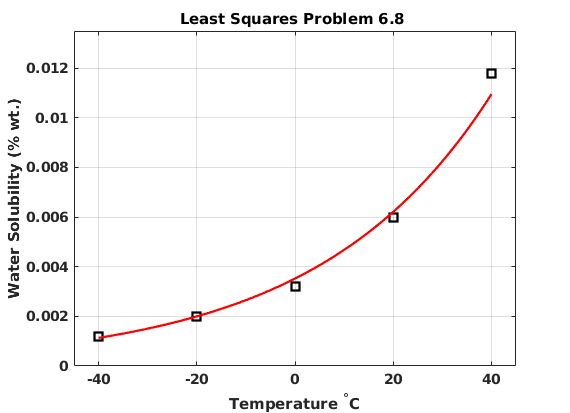
\includegraphics{lec14n-ex3.png}
\caption{Plot of least squares estimator for Example \#3.}
\label{fig:lec14n-ex3}
\end{marginfigure}





\chapter{Assignment \#5}
\label{ch:ass5}
\begin{fullwidth}
Find the general solution to the following differential equations in terms of Bessel Functions:
\begin{enumerate}
\item $4x^2u^{\prime \prime} + 4xu^{\prime} + \left(4x^2-25 \right)u = 0$

\vspace{1.0cm}

\item $ x^2u{\prime \prime}+xu^{\prime}+\left(9x^2-4\right)u = 0$

\vspace{1.0cm}

\item $x^2u^{\prime \prime}+xu^{\prime}-\left(16x^2+\frac{4}{9}\right)u = 0$
\end{enumerate}

\vspace{1.0cm}

\noindent Use the indicated change of variables to find the general solution of the given differential equation.
\begin{enumerate}[resume]
\item $x^2u^{\prime\prime}+2xu^{\prime}+\alpha^2x^2u = 0, \ \ u = x^{-\sfrac{1}{2}}v(x) $
\end{enumerate}

\vspace{1.0cm}

\noindent Use Equation \ref{eq:bessel-tool} to find the general solution of the following differential equation in terms of Bessel functions.
\begin{enumerate}[resume]
\item $xu^{\prime \prime} + 2u^{\prime} + 4u = 0$
\end{enumerate}

\end{fullwidth}

\chapter{Review \#1}
\label{ch:rev1n}
\begin{fullwidth}

\section{List of Topics}
\begin{enumerate}
\item Mathematical preliminaries:
\begin{enumerate}
\item Number representation.
\begin{enumerate}
\item Unsigned integer representations.
\item IEEE-754 floating point representation.
\end{enumerate}
\item Sources of error.

\item Background of Linear Algebra.
\begin{enumerate}
\item matrix/vector operations.
\item matrix properties.
\end{enumerate}
\end{enumerate}

\item Solution of Non-linear Equations.
\begin{enumerate}
\item Bisection method.
\item Newton's method (single equation and system of equations).
\item Secant method.
\item Steffen's method.
\item MATLAB built-in methods (single equation and system of equations).
\end{enumerate}

\item Solution of Linear System of Equations.

\begin{enumerate}
\item Gauss elimination with and without pivoting.
\item LU factorization with and without pivoting.
\item MATLAB built-in methods.
\item Error bounds for solution of linear systems of equations.
\item Iterative methods:
\begin{enumerate}
\item Jacobi, Gauss-Seidel, SOR.
\item MATLAB built-in methods including: \lstinline[style=myMatlab]{pcg} and \lstinline[style=myMatlab]{gmres} with preconditioning.
\end{enumerate}
\end{enumerate}

\end{enumerate}

\section{Review Questions}

\begin{enumerate}
\item Write down the sign bit, exponent bits, and first 6 bits of the mantissa for IEEE-754 double precision floating point representation of the number 2023.

\vspace{5.0cm}

\item Write down the number 81 in 32-bit unsigned integer format (little-endian layout).

\vspace{5.0cm}

\item Carry out 2 iterations of the secant method to find the root of $f(x) = x - 2e^{-x}$ starting with $x_1 = 0$ and $x_2 = 1$. (i.e. find $x_3$ and $x_4$)

\vspace{15.0cm}

\item Consider the following system of nonlinear equations:
\begin{align*}
-2x^3 + 3y^2 + 42 &= 0 \\
5x^2 + 3y^3 - 69 &= 0
\end{align*}
Using Newton's method for a system of equations and starting at $x=y=1$ write the linear system of equations you would need to solve to find $\Delta x$ and $\Delta y$ to update the estimated solution.


\vspace{4.0cm}

\item Using MATLAB's built-in function: \lstinline[style=myMatlab]{[L,U,P] = lu(A)} function, find the solution to the linear system of equations shown below:

\begin{equation*}
\bracketMatrixstack{
0 & 3 & 8 & -5 & -1 & 6 \\
3 & 12 & -4 & 8 & 5 & -2 \\
8 & 0 & 0 & 10 & -3 & 7 \\
3 & 1 & 0 & 0 & 0 & 4 \\
0 & 0 & 4 & -6 & 0 & 2 \\
3 & 0 & 5 & 0 & 0 & -6 
}
\bracketVectorstack{
x_1 \\
x_2 \\
x_3 \\
x_4 \\
x_5 \\
x_6
}
=
\bracketVectorstack{
34 \\
20 \\
45 \\
36 \\
60 \\
28
}
\end{equation*}
\end{enumerate}

\end{fullwidth}


\part{Orthogonal Functions and Fourier Series}
\chapter{Lecture 15 Interpolation with Lagrange Polynomials}
\label{ch:lec15n}
\section{Objectives}
The objectives of this lecture are to:
\begin{itemize}
\item Discuss the problem of interpolation and illustrate how it can be done with linear least squares.
\item Introduce Lagrange polynomials as a preferable strategy for interpolation.
\item Illustrate the techniques with a MATLAB example.
\end{itemize}
\setcounter{lstannotation}{0}

\section{Interpolation with Least Squares}

Interpolation is a lot like curve fitting except that we expect the estimator to be \emph{exact} at the given data points.  In principle this can be done with linear least squares.  For any given $n$ data points, we can construct a polynomial interpolant of degree $n-1$ that matches the given data exactly.

\vspace{0.15cm}

\noindent \textbf{Example: } Create a 4\textsuperscript{th} order interpolant for the following 5 data points using linear least squares.

\begin{table}
\begin{tabular}{|c|c|c|c|c|c|}
\hline
$x$ & 1 & 4 & 7 & 10 & 13 \\ \hline
$y$ & 2 & 6 & 4 & 8 & 10 \\ \hline
\end{tabular}
\end{table}

\vspace{0.2cm} 

\noindent MATLAB code to carry out this process is provided in the listing below:
\marginnote[2.0cm]{

\noindent \ref{lst:ann15n-1} This is slightly tricky but the effect is to create a matrix, $X$, whose columns comprise $x^{n}$ for $n \in [0,1,2,3,4,5]$.

\vspace{0.25cm}

\noindent \ref{lst:ann15n-2} This is also tricky; note, in particular, that the $x$ in this line of code is different from the $x$ in the data section.  The effect is to create an interpolant of the form:
$$\text{nthInterp}(x) = c(1) + c(2)x^1 + \cdots c(n)x^{n-1}$$
}
\begin{lstlisting}[style=myMatlab]
clear
clc
close 'all'
% Data
x = [1 4 7 10 13]';
y = [2 6 4 8 10]';
% Create least squares interpolant
N = length(x);
X = x.^(0:N); /*!\annotation{lst:ann15n-1}!*/
c = (X'*X)\(X'*y);
nthInterp = @(x) (x.^(0:N))*c; /*!\annotation{lst:ann15n-2}!*/
\end{lstlisting}

\noindent The data and least squares interpolant are presented in Figure \ref{fig:lec15n-ex-ls-interp}.  
\begin{marginfigure}
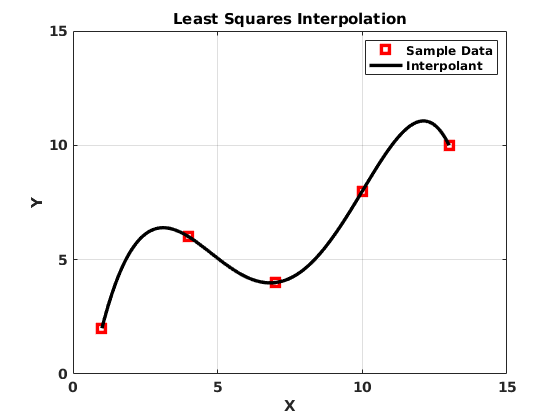
\includegraphics{lec15n-ex-ls-interp.png}
\caption{Least squares interpolation of data points.}
\label{fig:lec15n-ex-ls-interp}
\end{marginfigure}
Notice that, while the interpolant---as required---manages to pass through all of the data points, it is not an altogether great representation of the overall trend of the data.\sidenote{I suspect that  you would not want to really use this interpolant to estimate values between the data points.} Some other problems that are inherent to this approach:
\begin{enumerate}
\item As $n$ increases, the columns of \lstinline[style=myMatlab]{X} are more ``like'' each other.  As a result, the condition number of \lstinline[style=myMatlab]{(X'*X)} increases and, as we learned in Lecture 10, there is as a consequence greater numerical error in solving the linear system to find the coefficients.  In fact, when I execute this code in MATLAB, an error is issued due to the high condition number of \lstinline[style=myMatlab]{(X'*X)}:

\begin{figure}
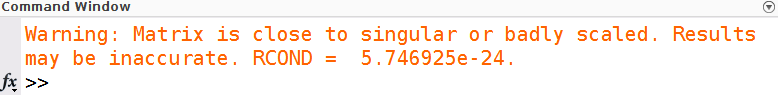
\includegraphics[width=0.75\textwidth]{lec15n-ex-ls-interp-warn.png}
\caption{Warning issued by MATLAB due to the high condition number of \lstinline[style=myMatlab]{(X'*X)}.}
\label{fig:lec15n-ex-ls-interp-warn}
\end{figure}

\item Solving a set of linear equations for the interpolating coefficients is inconvenient for some applications.  Working in a MATLAB environment we might forget that, generally speaking, solving a linear system of equations is complicated. 
\end{enumerate}

\noindent For applications later in the course, such as finite element methods, we will be very picky about the quality of interpolation functions and we will not be particularly interested in solving systems of linear equations on each domain that we hope to use such interpolations.  Luckily, there are better methods that avoid both of these problems.

\section{Lagrange Polynomial Interpolation}

Suppose we have 3 data points---$x_1$, $x_2$, and $x_3$---and we want to derive a 2\textsuperscript{nd} order polynomial interpolant, and we specify the polynomial as follows:
\begin{equation*}
f(x) = y = a_1(x-x_2)(x-x_3) + a_2(x-x_1)(x-x_3) + a_3(x-x_1)(x-x_2)
\end{equation*}
Notice the form of this polynomial; when we evaluate $f(x)$ at $x_1$, the first term on the right is the only non-zero term; when we evaluate $f(x_2)$, only the second term on the right is non-zero and similarly for when we evaluate $f(x_3)$.  This makes it easy to find values for $a_1$, $a_2$ and $a_3$.  Since
\begin{align*}
f(x_1) &= y_1 \\
&=a_1(x_1 - x_2)(x_1 - x_3) + a_2 \cancelto{0}{(x_1 - x_1)}(x_1 - x_3) + a_3\cancelto{0}{(x_1 - x_1)}(x_1 - x_2) \\
\Rightarrow a_1 &= \frac{y_1}{(x_1 - x_2)(x_1 - x_3)} 
\end{align*}
We can derive equations for $a_2$ and $a_3$ in the same way:
\begin{align*}
a_2 & = \frac{y_2}{(x_2 - x_1)(x_2 - x_3)} \\
a_3 & = \frac{y_3}{(x_3 - x_1)(x_3 - x_2)}
\end{align*}

\noindent Thus we have specified, what we will call, a Lagrange polynomial through these points:
\begin{equation*}
f(x) = \frac{(x - x_2)(x - x_3)y_1}{(x_1 - x_2)(x_1 - x_3)} + \frac{(x - x_1)(x-x_3)y_2}{(x_2 - x_1)(x_2 - x_3)} + \frac{(x - x_1)(x-x_2)y_3}{(x_3-x_1)(x_3 - x_2)}
\end{equation*}
In general, we construct the Lagrange polynomial as shown in Equation \ref{eq:lec15n-lagrange}:
\begin{equation}
f(x) = \sum\limits_{i=1}^{n} y_i L_i(x) = \sum\limits_{i=1}^{n} y_i \underbrace{\prod_{\substack{j=1 \\ j \ne i}}^{n} \frac{(x - x_j)}{(x_i - x_j)}}_{\substack{\text{Lagrange} \\ \text{function}}}
\label{eq:lec15n-lagrange}
\end{equation}
While this formulation avoids the aforementioned problems, it still can result in a low-quality interpolant.  It turns out that the quality of the interpolant depends on the number of points one hopes to interpolate and \emph{the spacing} of these points.  In particular, uniformly spaced interpolating points results in low quality interpolants.

Consider, as an example, following function:
\begin{equation*}
f(x) = \frac{8a^3}{x^2 + 4a^2}
\end{equation*} 
where $a$ is a parameter.  This is the so-called Witch of Agnesi\cite{WOA} problem and it is a classic test case for interpolation schemes.\cite{trefethen2} If we set $a=0.15$ and construct a Lagrange interpolant with uniformly spaced points, we get the result shown in Figure \ref{fig:lec15n-woa-uniform}.  The interpolation improves as $n$ increases everywhere except near the endpoints of the domain.  At the endpoints, the interpolation becomes worse.

%\begin{fullwidth}
\begin{figure}
\subfloat[]{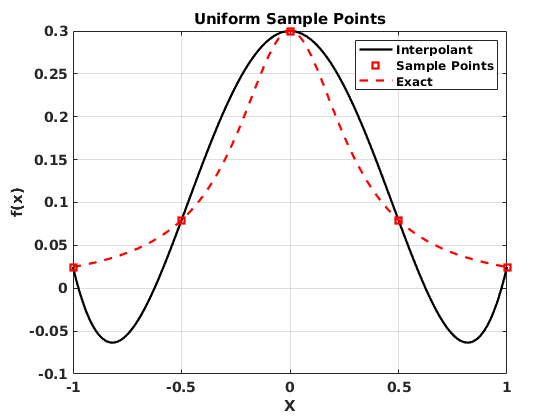
\includegraphics[width=2.25in]{lec15n-ex2-u-n5.png}}
\subfloat[]{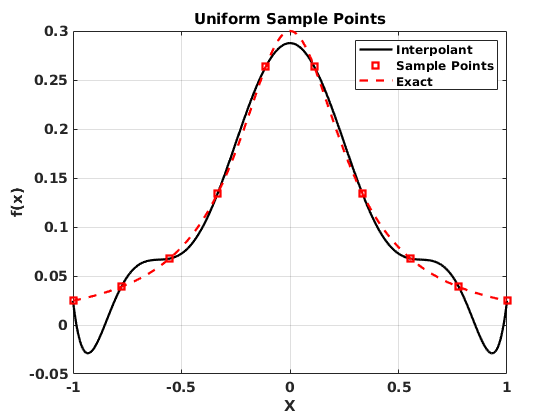
\includegraphics[width=2.25in]{lec15n-ex2-u-n10.png}}
\\
\subfloat[]{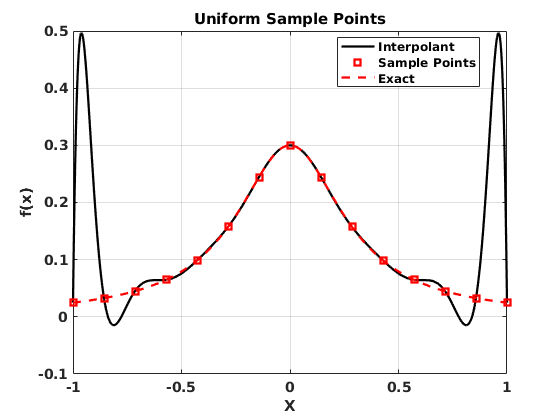
\includegraphics[width=2.25in]{lec15n-ex2-u-n15.png}}
\subfloat[]{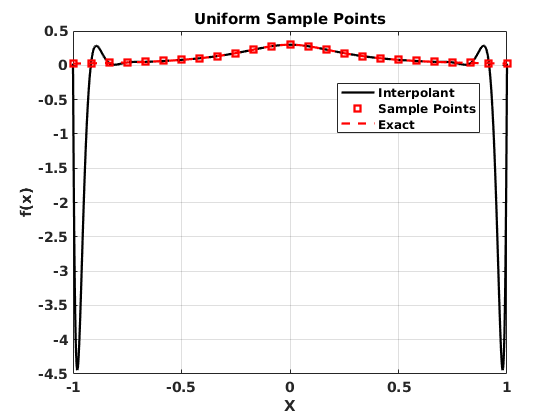
\includegraphics[width=2.25in]{lec15n-ex2-u-n25.png}}
\label{fig:lec15n-woa-uniform}
\caption[][0.0cm]{Lagrange interpolation with $n=5$, $n=10$, $n=15$, and $n=20$ uniformly spaced points.}
\end{figure}
%\end{fullwidth}
If instead of using uniformly spaced points, we choose particular set of non-uniformly spaced points, the quality of the interpolation is much improved.  In Figure \ref{fig:lec15n-woa-cheb} we select \emph{Chebyshev nodes} for interpolation.\sidenote{Chebyshev nodes, on the interval $x\in[-1,1]$ are given by:
$$x_k = \cos{\left(\frac{2k - 1}{2n}\pi \right)}, \ k=1,\dots,n$$
or for an arbitrary interval $x \in [a,b]$ via the following mapping:
$$x_k = \frac{1}{2}(a+b) + \frac{1}{2}(b-a)\cos{\left(\frac{2k - 1}{2n}\pi \right)}, \ k=1,\dots,n$$
} 
\begin{figure}
\subfloat[]{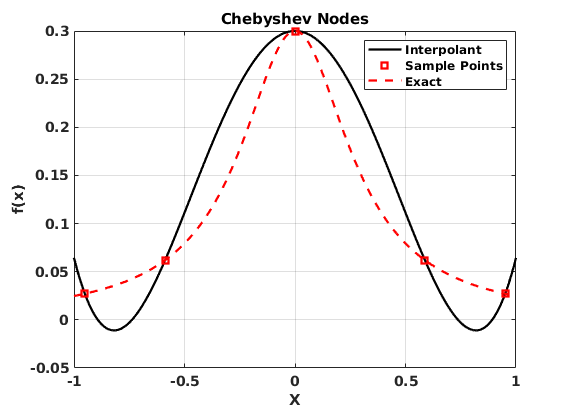
\includegraphics[width=2.25in]{lec15n-ex2-c-n5.png}}
\subfloat[]{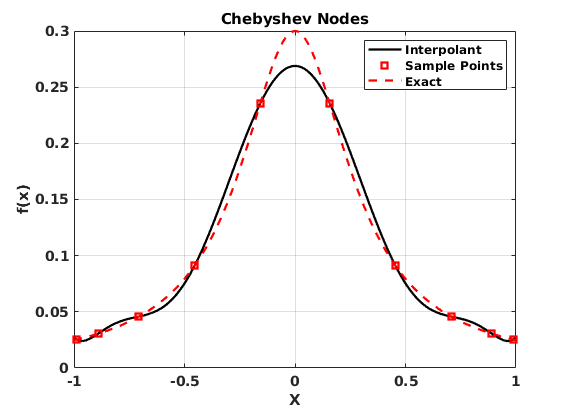
\includegraphics[width=2.25in]{lec15n-ex2-c-n10.png}}
\\
\subfloat[]{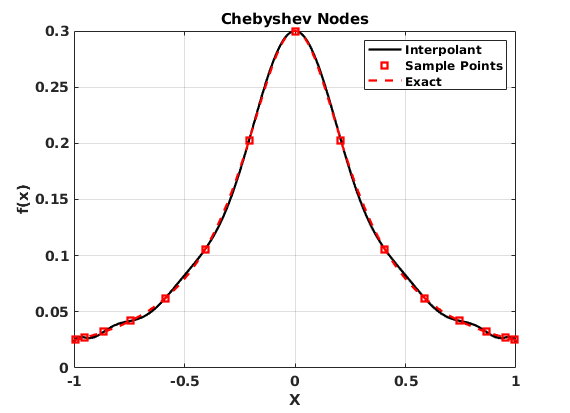
\includegraphics[width=2.25in]{lec15n-ex2-c-n15.png}}
\subfloat[]{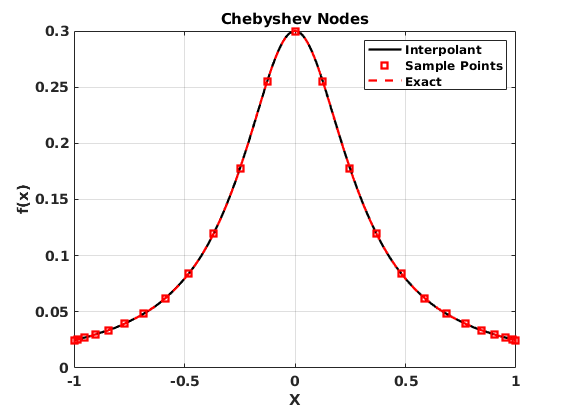
\includegraphics[width=2.25in]{lec15n-ex2-c-n25.png}}
\label{fig:lec15n-woa-cheb}
\caption[][0.0cm]{Lagrange interpolation with $n=5$, $n=10$, $n=15$, and $n=20$ points placed at Chebyshev nodes.}
\end{figure}
To be sure, there are many contexts in which the analyst, who is devising the interpolation scheme, is not at liberty to choose the sample points. In cases where you can choose the sample points, know that how you choose your points makes a difference.

\section{Matlab Example}
In this example, we will illustrate a case where the user does \emph{not} have a choice in the sample points.  Nonetheless, it will be worthwhile to show the MATLAB code so you can adapt it to a case of interest to you.

We will start by clearing out the workspace and loading the data we wish to interpolate.
\begin{lstlisting}[style=myMatlab,name=lec15n-ex2]
clear
clc
close 'all'

%% Load data
Strain = [0 0.4 0.8 1.2 1.6 2.0 2.4 2.8 3.2...
    3.6 4.0 4.4 4.8 5.2 5.6 6.0]';% dimensionless
Stress = [0 3.0 4.5 5.8 5.9 5.8 6.2 7.4 9.6...
    15.6 20.7 26.7 31.1 35.6 39.3 41.5]'; % MPa
\end{lstlisting}

Once the data is defined, we can create interpolations with both monomials and Lagrange polynomials.  

\begin{lstlisting}[style=myMatlab,name=lec15n-ex2]
%% N-th order Interpolation (monomials)

N = length(Strain);
X = Strain.^(0:N);
c = (X'*X)\(X'*Stress);
nthInterp = @(x) (x.^(0:N))*c;

%% Lagrange Interpolation
F = genLagrangePolyInterp(Strain,Stress);
\end{lstlisting}

Of course, all of the work for the Lagrange polynomial interpolation is packaged into the local function \lstinline[style=myMatlab]{genLagrangePolyInterp(X,Y)}.  The MATLAB code to make that happen is shown next.

\begin{lstlisting}[style=myMatlab,name=lec15n-ex2]
%% Local function for Lagrange polynomial
function F = genLagrangePolyInterp(X,Y)
% function F = genLagrangePoly(X,Y) generates a Lagrange  
% polynomial that may be used to interpolate a function
% inputs
% X = x-values of a function
% Y = f(X) for some function
%
% Outputs
% F - a function handle with the Lagrange interpolant

n = length(X); 

F = @(x) 0; % initialize the interpolant

for i = 1:n
    L = @(x) Y(i); % initialize the Lagrange Function
    for j = 1:n
        if j ~= i
            L = @(x) L(x).*((x - X(j))./(X(i) - X(j)));
        end
    end
    F = @(x) F(x)+L(x);
end
end
\end{lstlisting}

We can plot the resulting interpolants; these are shown in Figure \ref{fig:lec15n-ex3-monomial} and Figure \ref{fig:lec15n-ex3-lagrange} for monomial and Lagrange interpolation respectively.  As can be seen, the Lagrange interpolant is not great.  Nonetheless, the use of Lagrange polynomials for interpolation is a valuable tool, particularly for cases where the analyst can select the sample points for the interpolant.
\begin{marginfigure}
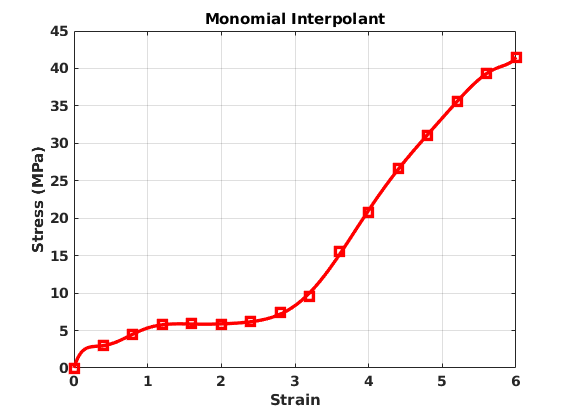
\includegraphics{lec15n-ex3-monomial.png}
\caption{Monomial interpolant for stress-strain data.}
\label{fig:lec15n-ex3-monomial}
\end{marginfigure}

\begin{marginfigure}
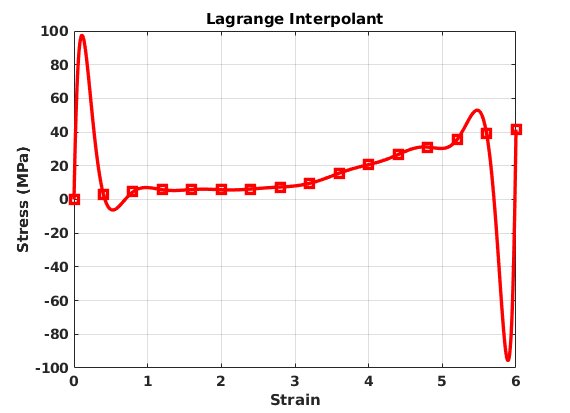
\includegraphics{lec15n-ex3-lagrange.png}
\caption{Lagrange interpolation for stress-strain data.}
\label{fig:lec15n-ex3-lagrange}
\end{marginfigure}


\chapter{Lecture 16 - Fourier Series}
\label{ch:lec16}
\section{Objectives}
\begin{itemize}
\item Review trigonometric Series.
\item Derive/show the formulas for expansion of a function as a Fourier series.
\item Discuss periodic extensiions of non-periodic functions, sine/cosine expansions, and convergence behavior.
\end{itemize}

\section{Review of Fourier Series}
In the last lecture we learned about orthogonal functions and sets of orthogonal functions.  We stated that most functions can be expressed as a linear combination of those orthogonal funcions:
\begin{equation*}
u(x) = \sum\limits_{n=0}^{\infty} c_n \phi_n
\end{equation*}
where $\phi_n$ are members of a set of orthogonal functions and $c_n$ are determined by:
\begin{equation*}
c_n = \frac{(u,\phi_n)}{||\phi_n||^2}\phi_n
\end{equation*} \index{Fourier Series}
You should already have experience with expansions such as this from your previous classes in differential equations in the form of Fourier series expansions.  In this case the orthogonal functions, $\phi_n(x)$, are:
\begin{equation*}
\left\{1,\cos{\frac{\pi x}{p}},\cos{\frac{2\pi x}{p}},\dots,\sin{\frac{\pi x}{p}}, \sin{\frac{2\pi x}{p}}, \dots \right\}
\end{equation*}
\marginnote{The function $\phi(x) = 1$ could also be written: $\cos{\frac{0 \pi x}{p}}$.}where $p$ indicates the \emph{period}.

That members of this set of functions are all mutually orthogonal can be directly shown; we will demonstrate this for the members of the form $\phi_n(x) = \cos{\sfrac{n \pi x}{p}}$; other cases are left for homework exercises.

\vspace{1.0cm}

\noindent\textbf{Example:} Show that functions of the form $\phi_n(x) = \cos{\frac{n\pi x}{p}}$ are orthogonal over the interval $x \in [-p,p]$:

\vspace{0.5cm}
\noindent Consider two functions, $\phi_n(x)$ and $\phi_m(x)$ where $m,n$ are integers and $m \ne n$.  The functions are orthogonal on the interval $x\in [-p,p]$ if $(\phi_n,\phi_m) = 0$.  From the definition of the inner product:\marginnote[0.5cm]{Here we use the identity: $\cos{(\alpha \pm \beta)} = \cos{\alpha}\cos{\beta} \mp \sin{\alpha}\sin{\beta}$. So that
\begin{align*}
\cos{\left(\alpha + \beta\right)} &= \cos{\alpha}\cos{\beta} - \sin{\alpha}\sin{\beta} \\
+\cos{\left(\alpha - \beta\right)} &= \cos{\alpha}\cos{\beta} + \sin{\alpha}\sin{\beta} \\
&= 2\cos{\alpha}\cos{\beta}
\end{align*}
and therefore
\begin{align*}
\cos{\alpha}\cos{\beta} &= \frac{1}{2}\left[\cos{\left(\alpha + \beta\right)} + \cos{\left(\alpha - \beta\right)}\right]
\end{align*}
}
\begin{align*}
(\phi_n,\phi_m) &= \int_{-p}^{p} \cos{\frac{n \pi x}{p}} \cos{\frac{m \pi x}{p}} \ dx \\
&= \frac{1}{2}\int_{-p}^{p} \cos{(n+m)\frac{\pi x}{p}} + \cos{(n-m)\frac{\pi x}{p}} \ dx \\
&= \frac{1}{2} \left[\frac{1}{n+m} \frac{p}{\pi}\sin{(n+m)\frac{\pi x}{p}}\Bigl|_{-p}^{p} + \frac{1}{n-m}\frac{p}{\pi}\sin{(n-m)\frac{\pi x}{p}}\Bigl|_{-p}^{p} \right] \\
&=0
\end{align*}
where the last terms are zero since we are evaluating the sine function at integer multiples of $\pi$.  This shows, at least, all of the cosine members are orthogonal.  For the case $m=n$ we get:\marginnote[1.0cm]{Rather than derive this rigorously, we will combine a tabulated result of standard integrals: $\int \cos^2 u \ du = \frac{1}{2}u + \frac{1}{4}\sin{2u}+C$, with $u$ substitution.}
\begin{align*}
\left(\phi_n,\phi_n \right) &= \int_{-p}^{p} \cos{\left(\frac{n \pi x}{p} \right)}^2 \\
&= \frac{p}{n \pi} \left[\frac{1}{2}\frac{n \pi x}{p} + \frac{1}{4} \sin{\frac{2 n \pi x}{p}} \right]\Bigl|_{-p}^{p} \\
&= \frac{p}{2} - \frac{-p}{2} \\
&= p
\end{align*}

\newthought{We can use} this infinite set of orthogonal functions to represent any other continuous function over the interval $[-p,p]$.  In your differential equations class you were taught to do this by using Equation \ref{eq:fourier-exp}.

\begin{equation}
f(x) = \frac{a_0}{2} + \sum\limits_{n=1}^{\infty}\left[a_n \cos{\frac{n \pi x}{p}} + b_n \sin{\frac{n \pi x}{p}} \right]
\label{eq:fourier-exp}
\end{equation}

\chapter{Lecture 17 - Generating and Plotting Fourier Series in MATLAB}
\label{ch:lec17}
\section{Objectives}
\begin{itemize}
\item Demonstrate how to carry out Fourier series expansions using MATLAB.
\item Give a qualitative demonstration of convergence behavior of Fourier series.
\item Demonstrate Cosine and Sine series expansions.
\end{itemize}
In this lecture, we will illustrate the process of Fourier series expansions with three examples.

\vspace{0.5cm}

\noindent\textbf{Example \#1:}
Carry out the Fourier series expansion of the function given in Equation \ref{eq:lec17-ex1}, illustrated in Figure \ref{fig:lec17-ex1-fx}
\begin{equation}
f(x) = 
\begin{cases}
0, & -\pi \le x < 0 \\
\pi - x, & 0 \le x \le \pi
\end{cases}
\label{eq:lec17-ex1}
\end{equation}
\begin{marginfigure}
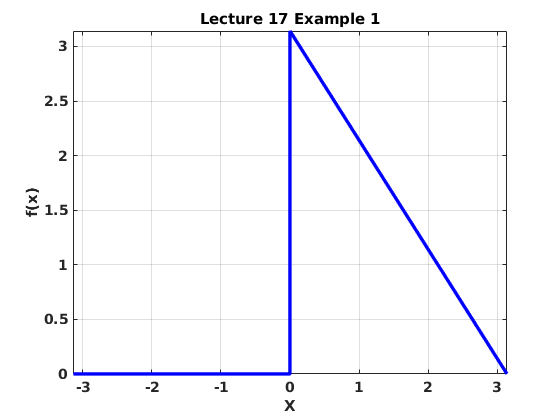
\includegraphics{lec17_ex1_fx.png}
\caption{Example \#1 $f(x)$.}
\label{fig:lec17-ex1-fx}
\end{marginfigure}
We wish to represent this function as:
\begin{equation*}
f(x) = \frac{a_0}{2} + \sum\limits_{n=1}^{\infty} \left[a_n \cos{\frac{n \pi x}{p}} + b_n \sin{\frac{n \pi x}{p}} \right]
\end{equation*}
where, in this case, $p = \pi$.  Even though we are only interested in the function in the interval $[-\pi, \pi]$, since the Fourier series represents the function in terms of a constant and an infinite linear combination of of periodic functions, we should think of the function that we are representing as periodic.\sidenote{This outlook will help us understand the convergence behavior of the Fourier series.}

We have everything we need; it is just a matter of calculating the coefficients from Equation \ref{eq:Fourier-Coeff}.  Rather than carrying out the calculations with pencil and paper we will use MATLAB.  In the listing below I will describe the code necessary to calculate Fourier coefficients through \lstinline{n=5}.

\begin{lstlisting}[name=lec17-ex1]
clear
clc
close 'all'

n = 5; % specify number of coefficients

f = @(x) ex1(x); 
p = pi; % specifiy period
\end{lstlisting}
We start, as always, by clearing out the workspace memory and command-prompt output and closing any open figures.  We also need to represent $f(x)$ in MATLAB; we will do this with a local function named \lstinline{ex1(x)}.\sidenote{Since inline functions must appear \emph{after} all of the other code in a MATLAB script file, I will provide the code for \lstinline{ex1(x)} last.}  

The integrals needed to determine the Fourier coefficients will be evaluated numerically using the MATLAB built-in function \lstinline{integral()}.\sidenote{This function has default signiature \lstinline{Q = integral(FUN,A,B)} approximates the integral of function \lstinline{FUN} over the interval \lstinline{A} to \lstinline{B} using global adaptive quadrature.  The error tolerances for this numeric integration algorithm can be specified by the user; in most cases we will use default values.  Students interested in how this works should take the Numerical Methods elective.} Let us start with $a_0$ which, as a reminder is computed by:
\begin{equation*}
a_0 = \frac{1}{p}\int_{-p}^{p} f(x) \ dx
\end{equation*}

\begin{lstlisting}[name=lec17-ex1]
a0 = (1/p)*integral(f,-p,p);
FF = @(x) a0/2;
\end{lstlisting}
The first line of the listing numerically evaluates $a_0$; the second line creates an anonymous function and initializes it to the first term in the Fourier expansion.

We will use a loop to construct the remaining terms in the Fourier expansion.\marginnote{Recall:
\begin{align*}
an &= \frac{1}{p}\int_{-p}^p f(x) \cos{\frac{n \pi x}{p}}\ dx \\
bn &= \frac{1}{p}\int_{-p}^p f(x) \sin{\frac{n \pi x}{p}}\ dx
\end{align*}
Note how you can practically read the equation directly from the MATLAB code.
}
\begin{lstlisting}[name=lec17-ex1]
for i = 1:n
an = (1/p)*integral(@(x) f(x).*cos(i*pi*x/p),-p,p);
bn = (1/p)*integral(@(x) f(x).*sin(i*pi*x/p),-p,p);
FF = @(x) FF(x) + an*cos(i*pi*x/p) + bn*sin(i*pi*x/p); 
end
\end{lstlisting}
Note in the last line where we append the newly computed terms to the Fourier series expansion \lstinline{FF(x)}.  Now we have a function, $\lstinline{FF(x)}$ that represents the Fourier series expansion with $n=5$ terms.  In the next listing we add the code to plot the function and verify that it makes sense.
\marginnote{Referring to the annotations:

\vspace{0.25cm}

\noindent \ref{lst:annotation1} Using \lstinline{sprintf()} allows us to combine the variable \lstinline{n} in the title string.  

\vspace{0.25cm}

\noindent \ref{lst:annotation2} Optional keyword-argument pairs such as \lstinline{'Linewidth',3}, \lstinline{'FontSize',16}, and \lstinline{'FontWeight','bold'} help make the plot and labels more readable.

\vspace{0.25cm}

\noindent \ref{lst:annotation3} Make a habit of using legends for graphs that include multiple data series. Once again, this makes the plot more readable.

\vspace{0.25cm}

\noindent \ref{lst:annotation4} The keyword \lstinline{gca} means ``get current axis''.  Calling the \lstinline{set()} function with keyword-argument pairs \lstinline{'FontSize',10} and \lstinline{'FontSize','bold'} sets the font size and weight for the axis markings.

\vspace{0.25cm}

\noindent In general it is important that your plots look good.

}

\begin{lstlisting}[name=lec17-ex1]
Nx = 1000;
X = linspace(-p,p,Nx);

plot(X,f(X),'-b',...
    X,FF(X),'--r',...
    'LineWidth',3)
title_str = sprintf('Example 1, n = %d',n);/*!\annotation{lst:annotation1}!*/
title(title_str,'FontSize',16,...
    'FontWeight','bold');
xlabel('X','FontSize',14,... /*!\annotation{lst:annotation2}!*/
    'FontWeight','bold');
ylabel('f(X)','FontSize',14,...
    'FontWeight','bold');
grid on
legend('f(x)','FF(x)')/*!\annotation{lst:annotation3}!*/
set(gca,'FontSize',12,...
    'FontWeight','bold');/*!\annotation{lst:annotation4}!*/
\end{lstlisting} \setcounter{lstannotation}{0}
The resulting Fourier series expansion is shown in Figure \ref{fig:lec17-ex1-n5}. If I increase the number of Fourier series terms in my expansion, I need only change \lstinline{n}; Figure \ref{fig:lec17-ex1-n15} shows the series expansion with \lstinline{n=15} terms.
\begin{marginfigure}
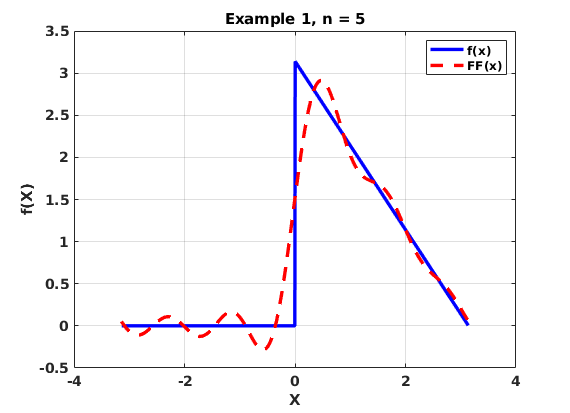
\includegraphics{lec17_ex1_n5.png}
\caption{Fourier series expansion with \lstinline{n=5}.}
\label{fig:lec17-ex1-n5}
\end{marginfigure}

\begin{marginfigure}
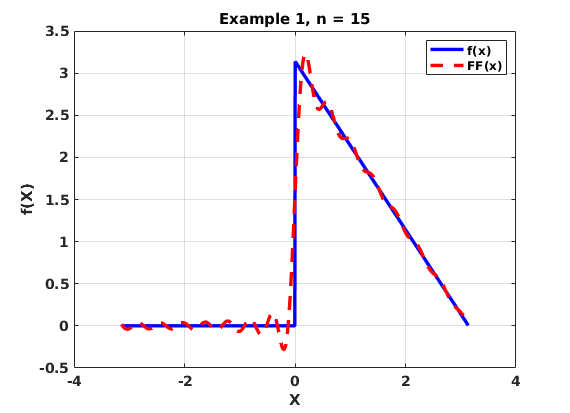
\includegraphics{lec17_ex1_n15.png}
\caption{Fourier series expansion with \lstinline{n=15}.}
\label{fig:lec17-ex1-n15}
\end{marginfigure} 
Some things to note about the resulting Fourier series representation of \lstinline{f(x)}:
\begin{enumerate}
\item As \lstinline{n} increases, \lstinline{FF(x)} generally ``looks more like'' \lstinline{f(x)}.  
\item At the discontinuity in \lstinline{f(x)}, the Fourier series representation appears to be converging on the midpoint between $f(x^-)$ and $f(x^+)$ as the theory says it should; and
\item The Fourier series representation near the point of discontinuity has ``wiggliness'' that doesn't go away as \lstinline{n} increases.
\item In particular, note the undershoot and overshoot of $f(x)$ to the left and right respectively of $f(0)$.  This is called ``Gibbs phenomena'' and it does not go away as \lstinline{n} increases but it moves closer to the point of discontinuity.  
\end{enumerate}
As Figure \ref{fig:lec17-ex1-n150} shows, as \lstinline{n} is increased, we can make \lstinline{FF(x)} arbitrarily close to \lstinline{f(x)} with the exception of the perturbations at the point of discontinuity.
\begin{marginfigure}
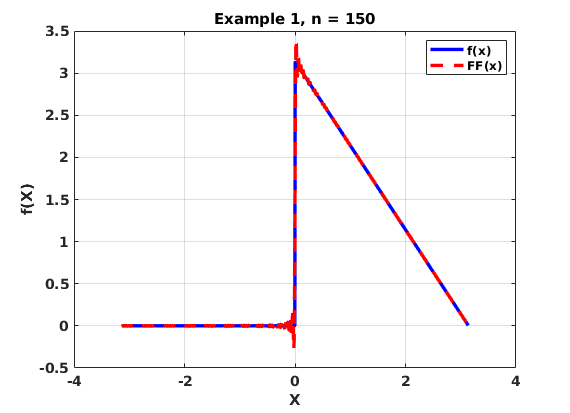
\includegraphics{lec17_ex1_n150.png}
\caption{Fourier series expansion with \lstinline{n=150}.}
\label{fig:lec17-ex1-n150}
\end{marginfigure}

\newthought{An important matter} that we have not yet dealt with is how to represent piecewise continuous functions like $f(x)$ in MATLAB.\sidenote{For whatever reason, piecewise continuous functions are intensively used in \emph{textbooks} on partial differential equations---I am not so sure that they are as important in real-life applications.}  As stated previously, we will use a \emph{local function} to do this.  The code is shown in the listing below.

\begin{lstlisting}[name=lec17-ex1]
%% Local functions 
function y = ex1(x) 
[m,n] = size(x); /*!\annotation{lst:annotation1-1}!*/
y = nan(m,n); /*!\annotation{lst:annotation1-2}!*/
for i = 1:length(x) /*!\annotation{lst:annotation1-3}!*/
    if (x(i) >= -pi) && (x(i) < 0) 
        y(i) = 0;
    elseif (x(i) >= 0) && (x(i) <= pi) /*!\annotation{lst:annotation1-4}!*/
        y(i) = pi - x(i);
    end
end
end
\end{lstlisting} \setcounter{lstannotation}{0}
Some notes on the annotations for this listing:

\vspace{0.25cm}

\noindent \ref{lst:annotation1-1}  We use the MATLAB built-in function \lstinline{size()} to get the dimensions of the input vector.  The return values \lstinline{[m,n]} give the number of rows and columns of \lstinline{x} respectively. For this function we are implicitly expecting \lstinline{x} to be a vector, but it can be either a row-vector or a column vector.

\vspace{0.25cm}

\noindent \ref{lst:annotation1-2} We construct the output vector \lstinline{y} using the \lstinline{nan()} function.  This line creates the vector \lstinline{y} to be the same size and shape as the input vector \lstinline{x}.  


\vspace{0.25cm}

\noindent \ref{lst:annotation1-3} We use the built-in function \lstinline{length()} to get the number of elements of \lstinline{x}.  This is a bit of a hack since, if \lstinline{x} were \textbf{\emph{not}} a vector, \lstinline{ex1(x)} would no longer work properly.\sidenote[][-5.0cm]{It would be a good idea to verify that the input \lstinline{x} is actually a vector.  MATLAB, like most other languages, includes features to enforce assumptions like this. The code: \lstinline{assert(min(size(x))==1,'x must be a vector')} would raise an error in MATLAB if the minimum dimension of \lstinline{x} is anything other than 1.  That would be one way to ensure \lstinline{x} is a vector.}

\vspace{0.25cm}

\noindent \ref{lst:annotation1-4} The symbol \lstinline{&&} is ``element-wise and''.  Pay attention to use of \lstinline{>=} and \lstinline{<=} operators to get the details of the intended function correct.

\vspace{0.5cm}

\noindent\textbf{Example \#2:}  Carry out the Fourier series expansion of the function given in Equation \ref{eq:lec17-ex2}, illustrated in Figure \ref{fig:lec17-ex2-fx}.
\begin{equation}
f(x) = 
\begin{cases}
-1, & -\pi \le x < 0 \\
1, & 0 \le x \le \pi
\end{cases}
\label{eq:lec17-ex2}
\end{equation}
\begin{marginfigure}[-6.0cm]
\includegraphics{lec17_ex2_fx.png}
\caption{Example \#2 $f(x)$.}
\label{fig:lec17-ex2-fx}
\end{marginfigure}
Fourier series expansions of this function are shown in Figures \ref{fig:lec17-ex2-n5} through \ref{fig:lec17-ex2-n150}.
\begin{marginfigure}[-1.0cm]
\includegraphics{lec17_ex2_n5.png}
\caption{Fourier series expansion with \lstinline{n=5}.}
\label{fig:lec17-ex2-n5}
\end{marginfigure}

\begin{marginfigure}
\includegraphics{lec17_ex2_n15.png}
\caption{Fourier series expansion with \lstinline{n=15}.}
\label{fig:lec17-ex2-n15}
\end{marginfigure}

\begin{marginfigure}
\includegraphics{lec17_ex2_n150.png}
\caption{Fourier series expansion with \lstinline{n=150}.}
\label{fig:lec17-ex2-n150}
\end{marginfigure}
Some notes:
\begin{enumerate}
\item As with the first example, the function has the Gibbs phenomena near the discontinuity at $x=0$.  
\item Also, as with the first example, the Gibbs phenomena does not go away as $n$ increases, but it gets more ``peaked'' and closer to the origin.
\item Unlike the first example, we get the Gibbs phenomena and wiggliness at the ends also.  This is because the Fourier series representation is periodic; the periodic extension of this function has discontinuities at the endpoints since $f(-\pi) \ne f(\pi)$.  
\item You should also note that this function is \emph{even}.  That means we expect $a_0$ and all values of $a_n$ to be equal to zero. If I modify the for-loop to output values for the $a_n$ coefficients I get all zeros.

\begin{lstlisting}
for i = 1:n
an = (1/p)*integral(@(x) f(x).*cos(i*pi*x/p),-p,p);
fprintf('a_%d = %g \n',i,an);
bn = (1/p)*integral(@(x) f(x).*sin(i*pi*x/p),-p,p);
FF = @(x) FF(x) + an*cos(i*pi*x/p) + bn*sin(i*pi*x/p); 
end
\end{lstlisting}
\end{enumerate}

%\begin{marginfigure}
%\includegraphics{lec17_ex2_an.png}
%\end{marginfigure}

\vspace{1.0cm}

\noindent\textbf{Example \#3:} Construct the Fourier series expansion of the function given in Equation \ref{eq:lec17-ex3-fx}.

\begin{equation}
f(x) = x^2, \ \ x \in[0,2]
\label{eq:lec17-ex3-fx}
\end{equation}

This function is not periodic and, unlike the previous examples, does not even span a symmetric interval about the origin.  In this case we will still use the same Fourier series formulas but we will construct a ``reflection'' about the origin.  This reflection can be \emph{even-}, \emph{odd-}, or it can be an \emph{identity-reflection} with respect to the y-axis; these correspond to the Cosine expansion, Sine expansion and the full Fourier series expansions.  These different expansion options are shown in Figure \ref{fig:lec17-ex3}.

\begin{figure}
\subfloat[]{\includegraphics[width=2in]{lec17_ex3_cos.png}}
\subfloat[]{\includegraphics[width=2in]{lec17_ex3_sin.png}} \\
\begin{center}
\subfloat[]{\includegraphics[width=2in]{lec17_ex3_full.png}}
\end{center}
\label{fig:lec17-ex3}
\caption{Even-, odd- and identity-reflection for $f(x)=x^2$.}
\end{figure}

\chapter{Assignment \#6}
\label{ch:ass6}
\begin{fullwidth}

Show that the given functions are orthogonal on the given interval.
\begin{enumerate}
\item $f_1(x) = e^{x}, \ f_2(x)=xe^{-x}-e^{-x}, \ \ x\in[0,2]$

\vspace{1.0cm}

\item $f_1(x) = x, \ f_2(x)=\cos{2x}, \ \ x\in\left[-\sfrac{\pi}{2},\sfrac{\pi}{2}\right]$
\end{enumerate}

\vspace{1.50cm}

\noindent Show that the given set of functions is orthogonal on the indicated interval.  Find the norm of each function in the set.
\begin{enumerate}[resume]
\item $\left\{\sin{x},\sin{3x},\sin{5x},\dots \right\}, \ \ x\in\left[0,\sfrac{\pi}{2}\right]$

\end{enumerate}

\vspace{1.5cm}

\noindent Use MATLAB to verify by numeric integration that the functions are orthogonal with respect to the indicated weight function on the given interval.

\begin{enumerate}[resume]
\item $H_0(x) = 1, \ H_1(x) = 2x, \ H_2(x)=4x^2-2; \ \ w(x)=e^{-x^2}, \ \ x\in(-\infty,\infty)$

\noindent\textbf{Note:} use the built-in function \lstinline{integral()} to do the numeric integration.  In MATLAB, $-\infty$ and $\infty$ are represented by \lstinline{-inf} and \lstinline{inf} respectively.
\end{enumerate}


\vspace{1.5cm}

\noindent Use MATLAB to construct the Fourier series expansion of the given function $f(x)$ on the given interval.  For each problem create a plot that shows: a) $f(x)$ along with b) the truncated Fourier series of $f(x)$ with \lstinline{N=5} and c) \lstinline{N=15} terms.  Also give the number to which the Fourier series expansion converges at any point(s) of discontinuity in $f(x)$. 

\begin{enumerate}[resume]
\item $f(x) = 
\begin{cases}
0, & -\pi < x < 0 \\
1, & 0 \le x < \pi
\end{cases}$


\vspace{1.0cm}

\item $f(x) = 
\begin{cases}
0, & -\pi < x < 0 \\
x^2, & 0 \le x < \pi
\end{cases}$

\vspace{1.0cm}

\item $f(x) = 
\begin{cases}
0, & -2 < x < 0 \\
-2, & -1 \le x < 0 \\
1, & 0 \le x < 1 \\
0, & 1 \le x < 2
\end{cases}$

\end{enumerate}

\vspace{1.5cm}

\noindent Determine whether the given function is even, odd, or neither.
\begin{enumerate}[resume]
\item $f(x) = x^2+x$

\vspace{1.0cm}

\item $f(x) =
\begin{cases}
x^2, & -1 < x < 0 \\
-x^2, & 0 \le x < 1
\end{cases}$
\end{enumerate}

\vspace{1.5cm}

\noindent Use MATLAB to expand the given function in an appropriate cosine or sine series.  For each function create a plot showing: a) $f(x)$ along with b) the truncated Fourier series of $f(x)$ with \lstinline{N=5} and; c) \lstinline{N=15} terms.

\begin{enumerate}[resume]
\item $f(x) = \left| x \right|, \ \ -\pi < x \pi$

\vspace{1.0cm}

\item $f(x) = 
\begin{cases}
x-1, & -\pi < x < 0 \\
x+1, & 0 \le x < \pi
\end{cases}$

\vspace{1.0cm}

\item $f(x) = 
\begin{cases}
1, & -2 < x < -1 \\
-x, & -1 \le x < 0 \\
x, & 0 \le x < 1 \\
1, & 1 \le x < 2
\end{cases}$

\vspace{1.0cm}

\item $f(x) = 
\begin{cases}
x, & 0 < x < \sfrac{\pi}{2} \\
\pi - x, & \sfrac{\pi}{2} \le x < \pi
\end{cases}$
\end{enumerate}

\end{fullwidth}

\chapter{Lecture 18 - Numeric Differentiation with Lagrange Polynomials}
\label{ch:lec18n}
\section{Objectives}
The objectives of this lecture are to:
\begin{itemize}
\item Review interpolation with Lagrange Polynomials
\item Describe and demonstrate numeric differentiation with Lagrange Polynomials
\item Illustrate use of non-uniform sample points
\end{itemize}
\setcounter{lstannotation}{0}

\section{Interpolation with Lagrange Polynomials}
As readers may recall from Lecture 15, we can approximate a function with Lagrange Polynomials using Equation \ref{eq:lec15n-lagrange} which is copied here for convenience:
\begin{equation*}
f_{\text{interp}}(x) = \sum\limits_{i=1}^{n} y_i L_i(x) = \sum\limits_{i=1}^{n} y_i \underbrace{\prod_{\substack{j=1 \\ j \ne i}}^{n} \frac{(x - x_j)}{(x_i - x_j)}}_{\substack{\text{Lagrange} \\ \text{function}}}
\end{equation*}
where $x_i$ are the points where the function is sampled and $y_i = f(x_i)$.  This is an interpolation which implies, at a minimum, that the interpolant $f_{\text{interp}}(x)$ is equal to $f(x)$ at the interpolating points.  What happens \emph{between the points}, however, is another matter entirely.  

\section{Differentiation of Lagrange Interpolant}
The strategy we will explore in this lecture is straight-forward.  In order to estimate the derivative of a function, we will first approximate the function with a polynomial (Lagrange) interpolant; then we will take the derivative of the interpolant.  

\newthought{To illustrate this} method, we will start with a relatively simple 3-point Lagrange interpolation:
\begin{equation*}
f_{\text{interp}}(x) = \frac{(x - x_2)(x - x_3)y_1}{(x_1 - x_2)(x_1 - x_3)} + \frac{(x - x_1)(x-x_3)y_2}{(x_2 - x_1)(x_2 - x_3)} + \frac{(x - x_1)(x-x_2)y_3}{(x_3-x_1)(x_3 - x_2)}
\end{equation*}
The derivative of this function is not too difficult, but it is somewhat messy:
\begin{fullwidth}
\begin{multline*}
\frac{df_{\text{interp}}}{dx} = y_1\left[\frac{1}{x_1 - x_2}\left(\frac{x - x_3}{x_1 - x_3}\right) + \frac{1}{x_1-x_3}\left(\frac{x - x_2}{x_1 - x_2} \right)\right] + \\ y_2\left[\frac{1}{x_2 - x_1}\left(\frac{x - x_3}{x_2 - x_3}\right) + \frac{1}{x_2 - x_3}\left(\frac{x - x_1}{x_2 - x_1}\right) \right] + y_3 \left[\frac{1}{x_3 - x_1}\left(\frac{x - x_2}{x_3 - x_2}\right) + \frac{1}{x_3 - x_2}\left(\frac{x - x_1}{x_3 - x_1}\right) \right]
\end{multline*}
\end{fullwidth}
We generalize this and encode in the notation used to describe Lagrange polynomials:
\begin{align}
\frac{df_{\text{interp}}}{dx} &= \sum\limits_{i=1}^{n}y_i \frac{d}{dx}L_{i}(x) = \sum\limits_{i=1}^{n}y_i\frac{d}{dx}\prod_{\substack{j=1 \\ j \ne i}}^{n} \frac{x - x_j}{x_i - x_j} \\ \nonumber
&= \sum\limits_{i=1}^{n}y_i\left[\sum\limits_{\substack{k = 1 \\ k \ne i}}^{n}\frac{1}{\left(x_i - x_k\right)} \prod_{\substack{j=1 \\ j \ne i \\ j \ne k}}^{n} \frac{\left(x - x_j\right)}{\left(x_i - x_j\right)} \right]
\end{align}
This formulation is admittedly messy, but with some patient MATLAB coding, it can be implemented without undue difficulty. A sample implementation is provided in the listing below.
\marginnote{

\vspace{4.5cm}

\noindent\ref{lst:ann18n-1} We initialize the derivative with Lagrange Interpolant with 0 - the additive identity.  As we add terms in line 32 of the listing, we do not need to make a special case for \lstinline[style=myMatlab]{i=1}.

\vspace{0.5cm}

\noindent\ref{lst:ann18n-2} Similarly here, we initialize the derivative of the Lagrange function with \lstinline[style=myMatlab]{dLp = @(x) 1}, which is the multiplicative identity, so a special case is not needed on line 23 and 24 where we include the next term of the product.
}
\begin{lstlisting}[style=myMatlab,name=lec18n-ex1]
function dF = genLagrangeInterpDeriv(X,Y)
% function dF = genLagrangeInterpDeriv(X,Y) generates the 
% derivative of a function using Lagrange Polynomial 
% interpolation.
% Inputs
% X = x-values of the function
% Y = f(X) for some function
%
% Outputs
% dF - a function handle with the derivative of 
% the Lagrange interpolant

n = length(X);
dF = @(x) 0; /*!\annotation{lst:ann18n-1}!*/

for i = 1:n
    dLi = @(x) 0;
    for k = 1:n
        if k ~= i
            dLp = @(x) 1; /*!\annotation{lst:ann18n-2}!*/
            for j = 1:n
                if ((j ~= i) && (j ~= k))
                    dLp = @(x) dLp(x).* ...
                        (x - X(j))./(X(i) - X(j));
                end
            end
            dLi = @(x) dLi(x) + ...
                (1./(X(i) - X(k))).*dLp(x);
        end
        
    end
    dF = @(x) dF(x) + dLi(x)*Y(i);
end
end
\end{lstlisting}

As can be seen just from the MATLAB implementation, this method is fundamentally different from finite difference formulas.  Using finite difference formulas, each equation only includes a few of the sample points while the Lagrange interpolant is a continuous function that includes \emph{all} sample points.  Recalling the discussion in Lecture 15 on Lagrange interpolation, you might expect that the quality of the numeric differentiation will depend not only on the number of sample points---where, in general, the quality of interpolation increases with more sample points---but also the \emph{distribution} of the sample points throughout the domain.  

\vspace{0.5cm}

\noindent\textbf{Example:} Use a Lagrange polynomials to numerically find the derivative of:
\begin{equation}
f(x) = \frac{1}{1+25x^2}
\label{eq:lec18n-f-ex1}
\end{equation}
Analytically, the derivative is:
\begin{equation*}
\frac{df}{dx} = \frac{-50x}{\left(1+25x^2\right)^2}
\end{equation*}
\begin{marginfigure}[-20.0cm]
\includegraphics{lec18n-ex1-woa-n11-uniform.png}
\caption{Numeric differentiation with $n=11$ uniformly spaced points.}
\label{fig:lec18n-ex1-woa-n11-uniform}
\end{marginfigure}
Using $n=11$ uniformly spaced sample points, the function and its numerical derivative is shown in Figure \ref{fig:lec18n-ex1-woa-n11-uniform}.  The numerical derivative is of very poor quality. For uniformly spaced points, however, the quality does not improve if $n$ is increased.  The result for $n=21$ is shown in Figure \ref{fig:lec18n-ex1-woa-n21-uniform}. If anything, the numeric derivative is worse.
\begin{marginfigure}[-14.0cm]
\includegraphics{lec18n-ex1-woa-n21-uniform.png}
\caption{Numeric differentiation with $n=21$ uniformly spaced points.}
\label{fig:lec18n-ex1-woa-n21-uniform}
\end{marginfigure}
\begin{marginfigure}[-4.0cm]
\includegraphics{lec18n-ex1-woa-n21-cheb.png}
\caption{Numeric differentiation with $n=21$ non-uniformly spaced points.}
\label{fig:lec18n-ex1-woa-n21-cheb}
\end{marginfigure}
In contrast, if we use non-uniformly spaced Chebychev points, as we did in Lecture 15, the quality of the numeric derivative is markedly better as we see in Figure \ref{fig:lec18n-ex1-woa-n21-cheb}.  Furthermore, if we increase the number of interpolation points, the quality of the numeric derivative improves still further as is shown in Figure \ref{fig:lec18n-ex1-woa-n51-cheb}.
\begin{marginfigure}[0.0cm]
\includegraphics{lec18n-ex1-woa-n51-cheb.png}
\caption{Numeric differentiation with $n=51$ non-uniformly spaced points.}
\label{fig:lec18n-ex1-woa-n51-cheb}
\end{marginfigure}
When we study Finite Element Methods in future lectures, we will find numeric differentiation with Lagrange Polynomials using non-uniform sample points to be a very important and powerful tool.


\chapter{Lecture 19 - Fourier-Bessel Series Expansions}
\label{ch:lec19}
\section{Objectives}
\begin{itemize}
\item Present the parametric Bessel equation as a Sturm-Liouville problem and derive the orthogonality relation.
\item Do an example to show expansion of a function in terms of Bessel functions.
\item Demonstrate use of the MATLAB function \lstinline{besselzero()}.
\end{itemize}

\section{Parametric Bessel Equation}
The parametric Bessel equation is a second-order linear, homogeneous differential equation that also fits within Sturm-Liouville theory.  As a reminder, the equation is:
\begin{equation*}
x^2u^{\prime \prime} + xu^{\prime} + \left(\alpha^2x^2-\nu^2\right)u = 0
\end{equation*}
and the general solution is given by:
\begin{equation*}
u(x) = c_1J_{\nu}(\alpha x) + c_2Y_{\nu}(\alpha x)
\end{equation*}

\newthought{The solutions,} $J_{\nu}(\alpha x)$ and $Y_{\nu}(\alpha x)$ are, of course, linearly independent but they also are orthogonal with respect to some weight function $p(x)$ and we can use them to construct an orthogonal function expansion in exactly the same way we did with Fourier series.  That is what we will do in this lecture.  To accomplish this we want to put the parametric Bessel equation in self-adjoint form and we will proceed in this effort just as we did in the last lecture.

\vspace{0.5cm}

\noindent Let us first put the parametric Bessel equation in standard form:\marginnote{It may not be clear immediately that $\lambda$ corresponds to values of $\alpha$ but that is the correct inference; when we do the orthogonal function expansion with Bessel functions it will be more clear why that is the case.}
\begin{align*}
a(x)u^{\prime \prime} + b(x)u^{\prime} + \left[c(x)+\lambda d(x) \right] u &= 0 \\
x^2u^{\prime \prime} + xu^{\prime} + \left[-\nu^2 + \alpha^2 x^2\right]u &=0
\end{align*}
so, $a(x) = x^2$, $b(x)=x$, $c(x) = -\nu^2$, and $d(x)=x^2$.

\vspace{0.25cm}

\noindent Next we will compute $r(x)$:
\begin{align*}
r(x) &= e^{\int \frac{b(x)}{a(x)} \ dx} \\
&= e^{\int \frac{x}{x^2} \ dx} \\
&= e^{\int \frac{1}{x} \ dx} \\
&= e^{\ln{x}} \\
&= x
\end{align*}

\vspace{0.25cm}

\noindent Now we compute $q(x)$:
\begin{align*}
q(x) &= \frac{c(x)}{a(x)}r(x) \\
&= \frac{-\nu^2}{x^2}x \\
&= -\frac{\nu^2}{x}
\end{align*}

\vspace{0.25cm}

\noindent Then $p(x)$:
\begin{align*}
p(x) &= \frac{d(x)}{a(x)}r(x) \\
&=\frac{x^2}{x^2}x \\
&= x
\end{align*}
So the self-adjoint form of the parametric Bessel equation is:\marginnote{Admittedly, the real reason why we want to do this is to obtain the weight function $p(x)$ which, in this case is $p(x)=x$.}
\begin{equation*}
\frac{d}{dx}\left[x u^{\prime} \right] + \left(-\frac{\nu^2}{x} + \alpha^2 x \right)u = 0
\end{equation*}
The corresponding orthogonality relation is shown in Equation \ref{eq:fb-ortho}\marginnote{Like other Sturm-Liouville problems we will find that there are infinitely many distinct eigenvalues, $\lambda_n$, which for this equation we will refer to as $\alpha_n$.  Note the weight function $x$ now appears in the inner product.}
\begin{equation}
\int_{a}^{b}J_{\nu}(\alpha_n x) J_{\nu}(\alpha_m x) x \ dx = 0, \ \ n \ne m
\label{eq:fb-ortho}
\end{equation}
where $a$ and $b$ are the bounds of the interval on which orthogonality is expressed.

\vspace{0.5cm}

\noindent\textbf{Example:} Expand $f(x)=x, \ 0<x<3$, in a Fourier-Bessel series, using Bessel functions of order $\nu=1$ that satisfy the boundary condition $J_{1}(3\alpha)=0.$\marginnote[-1.25cm]{Remember that it is the \emph{boundary conditions} that allow us to determine the eigenvalues.}

\vspace{0.25cm}
\begin{marginfigure}
\includegraphics{lec19_bessel1_plot.png}
\label{fig:lec19-bessel}
\caption{Bessel functions of order 1.}
\end{marginfigure}
\noindent So what we want is:
\begin{equation*}
f(x) = x = \sum\limits_{n=1}^{\infty}c_n J_{1}\left(\alpha_n x\right)
\end{equation*}
Note that we omit Bessel functions of the second kind, $Y_n(x)$, because as is shown in the figure, they diverge to negative infinity as $x$ goes to zero.  This \emph{implicit boundary condition}, where one solution of the differential equation diverges at the problem boundary, often needs to be considered when solving boundary value problems.

The other boundary condition applies at $x=3$: $J_{1}(3\alpha_n) = 0$ or, put differently, we select the values of $\alpha_n$ such that $3\alpha_n$ is a root of $J_{1}(x)$.  While our plot of $J_1(x)$ does not extend out to infinity, it turns out that $J_1(x)$ has infinitely many roots and we need to find them.

\subsection{Interlude on Open-Source Software}
At some point in time in your life as an engineer it is inevitable that a problem will arise that you are not prepared to tackle yourself. The tools you have been given to do your job do not fully answer to the task at hand.  This is one such occasion.  We need to find the roots of $J_1(x)$.  \emph{You} know those values exist but you don't know what they are and it turns out that MATLAB does not (at this time) have any built-in functions to give you the roots of such functions.\sidenote[][-2.0cm]{MATLAB \emph{does} have built-in functions to represent several types of Bessel functions; $J_{\nu}(x)$ and $Y_{\nu}(x)$ are represented, respectively, by \lstinline[style=myMatlab]{besselj(nu,x)} and \lstinline[style=myMatlab]{bessely(nu,x)}. We will learn about more Bessel functions in future lectures.}

Some options available to you include:
\begin{enumerate}
\item Go to the library and check out a book that tabulates some roots of $J_{1}(x)$---possibly also including scads of additional Bessel function lore\cite{bowman2012introduction}---and enter the desired roots by hand into your MATLAB code.
\item Implement an algorithm to find the roots of $J_1(x)$, possibly using a root-finding tool in MATLAB such as \lstinline[style=myMatlab]{fzero()} or \lstinline[style=myMatlab]{fsolve()}.
\item Find a third-party function or library that has already been written that solves the problem.
\end{enumerate}
In this case we will take the last option since, it turns out, someone has already solved this problem for us\marginnote[-0.5cm]{The Fourier-Bessel expansion that we are learning about in this lecture is a standard element in the analytical methods repertoire; \emph{of course} someone else has already figured out how to find the roots of Bessel functions.} and it is a safe bet that they did a better job than what we would be prepared to do.  The MATLAB file exchange is an online repository where people can obtain and share code that they find useful.\sidenote{Note that a (free) MathWorks account is required to use the MATLAB file exchange.}

\newthought{Regarding Open-Source} software:
We have a lot of experience with proprietary software. From operating systems like Microsoft Windows or Apple's IOs to office productivity tools like Microsoft Word or Excel, to valuable and important engineering tools like MATLAB or COMSOL.  We also have experience with free software, such as many applications that you download onto your smartphones.  I want to write a few words in hopes of dispelling any negative connotations that you may have developed in relation to open-source software in comparison to proprietary software.
\begin{itemize}
\item Scientists and engineers of all types---not just computer scientists---write and share software in an open-source framework.  Online repositories like GitHub and GitLab are meant expressly for developing code in an open and collaborative way and then sharing the results freely.
\item ``open-source'' ensures the source code is available.  Sometimes the code is also free but that is not the essential part.\sidenote{Think: ``free speech'', not ``free beer.''}

\item Open-source software is a \emph{hugely} important contribution to science.  Free and open-source tools like
\begin{itemize}
\item the programming languages that have been a part of the scientific computing landscape for generations.  Examples include Python, C++, Java and FORTRAN among others.
\item OpenMC\cite{ROMANO201590} - a powerful particle transport simulation tool similar to MCNP.
\item MOOSE - \underline{M}ulti-physics \underline{O}bject-\underline{O}riented \underline{S}imulation \underline{E}nvironment\cite{lindsay2022moose} combines the open-source finite element library libMesh\cite{kirk2006libmesh} and the \underline{P}ortable, \underline{E}xtensible \underline{T}oolkit for \underline{S}cientific \underline{C}omputation (PETSc)\cite{petsc-user-ref} along with a host of other free, open-source libraries to create an enormously powerful and flexible tool-set that is used to create the majority of all new multi-physics nuclear analysis codes in the United States.\sidenote{For a list of current applications tracked by the MOOSE development team see: \url{https://mooseframework.inl.gov/application_usage/tracked_apps.html}.  Not all of these codes are open-source, but they have all been created with open-source tools.}
\end{itemize} 
\item As the previous item should help illustrate, open-source software can be of very high quality.  The developers of MOOSE-based applications at the Department of Energy labs are highly trained scientists following nuclear quality assurance standards to ensure that the resulting software tools work correctly and do what they are supposed to do. 
\end{itemize}
The \LaTeX\ tools and almost all of the other software on the computer used to prepare this manuscript, including the Linux operating system, are free and open-source software.\sidenote{MATLAB is a notable exception to this list.  There is a free and open-source alternative called Octave. \url{https://octave.org/} } If you have any interest in scientific computing, now is a good time to develop an interest in open-source software.

\subsection{Back to the Example}
We want to expand $f(x)=x$ for $0<x<3$ in a Fourier-Bessel series expansion using Bessel functions of the first kind of order 1 that satisfy the boundary condition: $J_{1}(3\alpha_n)=0$.  We will use MATLAB along with the function \lstinline[style=myMatlab]{besselzero()} that we obtained from the MATLAB file exchange to carry out this task. In particular we will compute the truncated expansion with $N=15$ terms:
\begin{equation*}
f(x) = x = \sum\limits_{n=1}^{15}c_n J_1\left(\alpha_n x\right)
\end{equation*}

\begin{enumerate}
\item Use \lstinline[style=myMatlab]{besselzero()} to get $\alpha_1,\alpha_2,\dots,\alpha_N$ for our expansion.

\begin{lstlisting}[name=lec19_ex, style=myMatlab]
clear
clc
close 'all'

N = 15; % number of eigenvalues
a = 0; b = 3; % bounds of the domain
nu = 1; kind = 1;
k = besselzero(nu,N,kind); % get roots  /*!\annotation{lst:annotation19-1}!*/
alpha = k/b;  /*!\annotation{lst:annotation19-2}!*/
\end{lstlisting}
\marginnote[-1.5cm]{\ref{lst:annotation19-1} \lstinline[style=myMatlab]{besselzero()} takes up to three arguments; the first,$\nu$, is the order of the Bessel function; the second is the number of roots requested; the third is to indicate the \emph{kind}---first or second---of Bessel function for which you want the roots.

\vspace{0.25cm}
\ref{lst:annotation19-2} since $J_1\left(\alpha_n 3\right) = k_n$ where $k_n$ is the n\textsuperscript{th} root of $J_1$, $\alpha_n$ must be equal to $\sfrac{k_n}{3}$.

}

Now we have the first \lstinline{N=15} values of $\alpha_n$.

\item Compute the coefficients of the expansion $c_n$.  As with the Fourier series, we do this by multiplying both sides of our equation by an orthogonal function \emph{and the weight function } $p(x)=x$ and integrating. For example, to get $c_1$, we do the following:
\begin{align*}
f(x) = x &= c_1 J_1\left(\alpha_1 x\right) + c_2 J_1 \left(\alpha_2 x\right) + \cdots \\
\int_0^3 x J_1\left(\alpha_1 x\right) x \ dx &= c_1 \int_0^3 J_1\left(\alpha_1 x\right)^2 x \ dx + c_2 \underbracket{\int_0^3 J_1\left(\alpha_2 x \right) J_1 \left( \alpha_1 x \right) x \ dx}_{=0 \ \text{by orthogonality}} + \cdots \\
\Rightarrow c_1 &= \frac{\int_0^3 x J_1\left(\alpha_1 x\right) x \ dx}{\int_0^3 J_1\left(\alpha_1 x\right)^2 x \ dx}
\end{align*}
where we recall that the weight function for the orthogonality relation for the Bessel equation is $p(x)=x$.  For the calculation of $c_1$ all of the remaining terms are zero due to the weighted orthogonality of the eigenfunctions $J_1\left(\alpha_n x \right)$.  We repeat the process for all values of $c_n$ and, in MATLAB, we implement this process in the form of a loop.
\marginnote[3.0cm]{
\ref{lst:annotation19-3} these three lines are actually one long line of MATLAB that calculates the coefficients:
\begin{equation*}
c_n = \frac{\int_0^3 x J_1\left(\alpha_1 x\right) x \ dx}{\int_0^3 J_1\left(\alpha_1 x\right)^2 x \ dx}
\end{equation*}
}
\begin{lstlisting}[name=lec19_ex,style=myMatlab]
f = @(x) x; 
cn = nan(N,1); % store the coefficients (optional)

FB = @(x) 0; % initialize the Fourier-Bessel expansion
for n = 1:N
    % compute the i-th coefficient
    cn(n) =...
     integral(@(x) f(x).*besselj(nu,alpha(n)*x).*x,a,b)./... /*!\annotation{lst:annotation19-3}!*/
     integral(@(x) x.*besselj(nu,alpha(n)*x).^2,a,b);
    % update the Fourier-Bessel expansion
    FB = @(x) FB(x) + cn(n)*besselj(nu,alpha(n)*x); 
end
end
\end{lstlisting}
\end{enumerate}
We are now ready to plot the resulting Fourier expansion.\marginnote[0.75cm]{
\ref{lst:annotation19-4} Create a vector to represent the $x$-axis.}

\begin{lstlisting}[name=lec19_ex,style=myMatlab]
Nx = 1000;
X = linspace(a,b,Nx); /*!\annotation{lst:annotation19-4}!*/

figure(1)
plot(X,FB(X),'-b','LineWidth',3);
xlabel('X','fontsize',14,'fontweight','bold');
ylabel('f(X)','fontsize',14,'fontweight','bold');
titlestr = sprintf('Fourier-Bessel expansion, N = %d',N);
title(titlestr,'fontsize',16,'fontweight','bold');
grid on
set(gca,'fontsize',12,'fontweight','bold');

\end{lstlisting}
\begin{marginfigure}
\includegraphics{lec19_ex1_N15.png}
\caption{Fourier-Bessel expansion of $f(x)=x$.}
\end{marginfigure}
The Fourier-Bessel expansion of $f(x)=x$ with $N=15$ is shown in the figure.  Note that the expansion for $N=15$ looks pretty rough. There are many wiggles through the domain and the expansion drops suddenly to zero as the function approaches $x=3$.  The reason for this is that \emph{it had to.}  We are building the expansion with orthogonal functions that are all equal to zero at $x=3$.  Of course $f(x)=x$ is equal to 3 at $x=3$ so something had to give.  

\begin{marginfigure}
\includegraphics{lec19_ex1_N150.png}
\caption{Fourier-Bessel expansion of $f(x)=x$.}
\label{fig:lec19-ex1-n150}
\end{marginfigure}
We can improve the quality of the expansion by taking more terms.  Luckily, since we are using a computer, it is no problem at all to simply increase $N$; the computer does the same thing, just more of it.  The result is shown in Figure \ref{fig:lec19-ex1-n150} where the wiggliness remains---including the Gibbs phenomena we saw with Fourier series---but overall the representation is much more exact.

\section{Measuring Expansion Accuracy}
There is a straight-forward way to be more precise when we speak of the accuracy of an orthogonal function expansion.  A frequently used relative error measure is shown in Equation \ref{eq:lec19-rel-err}.

\begin{multline}
\text{Relative error} = \frac{\left(f(x) - FB(x), f(x)-FB(x)\right)}{\left(f(x),f(x)\right)} = \cdots \\ \frac{\int_a^b \left(f(x)-FB(x)\right)^2 \ dx}{\int_a^b f(x)^2 \ dx}
\label{eq:lec19-rel-err}
\end{multline}
\begin{marginfigure}
\includegraphics{lec19_ex1_converge.png}
\caption{Convergence of the Fourier-Bessel expansion of $f(x)=x$.}
\label{fig:lec19-converge}
\end{marginfigure}
MATLAB code for quantitatively measuring the relative error as the number of terms increases is shown below.  From Figure \ref{fig:lec19-converge} we can see that, as expected, the relative error steadily goes down.\sidenote{Note that it is conventional to show convergence graphs such as this on a log-log plot.  Eventually, we should expect errors in the determination of Bessel function roots and/or errors in carrying out the numeric integration to prevent further reduction in relative error.} 
%\begin{fullwidth}
\begin{lstlisting}[name=lec19-converge,style=myMatlab]
clear
clc
close 'all'

N = 500; % number of eigenvalues
a = 0; b = 3; % bounds of the domain
nu = 1; kind = 1;
k = besselzero(nu,N,kind); % get roots
alpha = k/b;

f = @(x) x; 
cn = nan(N,1); % store the coefficients (optional)
rel_err = nan(N,1); 

FB = @(x) 0; % initialize the Fourier-Bessel expansion
for n = 1:N
    % compute the i-th coefficient
    cn(n) =...
        integral(@(x) f(x).*besselj(nu,alpha(n)*x).*x,a,b)./...
        integral(@(x) x.*besselj(nu,alpha(n)*x).^2,a,b);
    % update the Fourier-Bessel expansion
    FB = @(x) FB(x) + cn(n)*besselj(nu,alpha(n)*x);

    % calculate sqruare norm of the relative "error"
    err_fn = @(x) FB(x) - f(x); 
    rel_err(n) = integral(@(x) err_fn(x).^2,a,b)./...
        integral(@(x) f(x).^2,a,b); 
end

figure(1)
loglog(1:N,rel_err,'-b',...
    'LineWidth',3);
title('\textbf{Convergence of Fourier-Bessel Expansion of } $$f(x)=x$$',...
    'Interpreter','latex');
ylabel('Relative Error','FontSize',14,...
    'FontWeight','bold');
xlabel('Number of Terms','FontSize',14,...
    'FontWeight','bold');
grid on
set(gca,'FontSize',12,'FontWeight','bold');
\end{lstlisting}
%\end{fullwidth}



\chapter{Lecture 20 - Gauss Quadrature}
\label{ch:lec20n}
\section{Objectives}
The objectives of this lecture are to:
\begin{itemize}
\item Define Gauss-Legendre quadrature and illustrate its convergence properties
\item Provide a derivation to explain how and why Gauss quadrature works
\end{itemize}
\setcounter{lstannotation}{0}

\section{Gauss-Legendre Quadrature}
Gauss-Legendre quadrature, from here-on-out referred to simply as Gauss quadrature, is similar to Newton-Cotes integration formulas in its overall algorithmic strategy:
\begin{itemize}
\item Approximate $f(x)$ by some other function, $g(x)$, that is in some way ``close'' to $f(x)$; and
\item Integrate that function exactly.
\end{itemize}
The main differences are:
\begin{enumerate}
\item Gauss quadrature schemes use a different measure to determine if $g(x)$ is ``close'' to $f(x)$.  In Newton-Cotes formulas, $g(x)$ was forced to be equal to $f(x)$ at pre-selected locations.  Gauss quadrature measures closeness in an integral sense as shown in Equation \ref{eq:lec20n-gq-close}.
\begin{equation}
\int_{a}^{b}\left[f(x) - g(x)\right]g(x) \ dx = 0
\label{eq:lec20n-gq-close}
\end{equation}
\marginnote[-1.0cm]{If $g(x)$ is close to $f(x)$, then the integral in Equation \ref{eq:lec20n-gq-close}, which we can think of as an inner product between $g(x)$ and the ``error'' $f(x) - g(x)$, will be small.}
\item Gauss quadrature does not require $g(x)$ to match $f(x)$ at any pre-determined number of locations in the interval, but it does call for sampling $f(x)$ at a number of discrete points throughout the interval much like trapezoidal and Simpson's rule does.  The location of these sample points (often called \emph{integration points} or \emph{Gauss points}) is a key factor to the accuracy that Gauss quadrature can achieve.
\end{enumerate}

In this lecture we will discuss two versions of the Gauss quadrature algorithm.  First, we will describe the algorithm in a recipe-like way without any discussion regarding the theory or why it all works.  After that is out of the way, a full derivation will be presented so that readers will know exactly how and why the method works.

\section{The Short Version}
In Gauss quadrature, the definite integral of a function $f(x)$ over an interval $[-1,1]$ is approximated by Equation \ref{eq:lec20n-gq-short}.
\begin{equation}
\int_{-1}^{1} f(x) \ dx \approx \sum\limits_{i=1}^{N}w_i f(x_i)
\label{eq:lec20n-gq-short}
\end{equation}
Since we generally do not want to integrate functions only from $x\in[-1,1]$, we will linearly map the desired domain, $[a,b]$, onto the reference domain, $t \in [-1,1]$, as follows:\marginnote{Notice that at $x(t=-1) = a$, and $x(t=1) = b$.}
\begin{align*}
x(t) &= \frac{1}{2}\left[(b-a)t + a + b \right] \\
dx &= \frac{1}{2}(b-a) \ dt
\end{align*}
Substituting this into the equation above gives us:
\begin{equation}
\int_{a}^{b}f(x) \ dx = \int_{-1}^{1}f(x(t))\frac{b-1}{2} \ dt \approx \sum\limits_{i=1}^{n}w_i f(x(t_i))\frac{b-a}{2}
\label{eq:lec20n-gp-formula}
\end{equation}

\begin{marginfigure}
\includegraphics{lec20n-gp-and-weights.png}
\caption{Published Gauss points and weights up to $n=6$.}
\label{fig:lec20n-gp-and-weights}
\end{marginfigure}
Values for Gauss points and weights are commonly tabulated, as shown in Figure \ref{fig:lec20n-gp-and-weights}. Engineers wanting to use Gauss quadrature incorporate those values into their code in some appropriate way and carry out the numeric integration.

The convergence of Gauss quadrature depends on the number of Gauss points used: order $2n-1$ for $n$ points.  If you want faster convergence, simply add more points.\sidenote{This is referred to as \emph{exponential convergence.}}  Figure \ref{fig:lec20n-gq-convergence} shows the convergence behavior of Gauss quadrature for calculating the integral:
\begin{equation*}
\int_{-3}^3 e^{-x^2} \ dx
\end{equation*}
\begin{marginfigure}
\includegraphics{lec20n-gq-convergence.png}
\caption{Convergence behavior of Gauss quadrature.}
\label{fig:lec20n-gq-convergence}
\end{marginfigure}
This convergence result was obtained using a single interval for the integral.  It is, of course, possible to break the domain into multiple sub-domains and carry out the integral using Gauss quadrature for each sub-domain and then sum the result.  In that case, convergence depends on the number of Gauss points used on each sub-domain.  The error will be $\mathcal{O}(h^{2n-1})$ where $h$ is the size of each sub-domain and $n$ is the number of Gauss points used on each sub-domain.


\section{The Long Version}

For Gauss quadrature, we approximate the integral of $f(x)$ as follows:
\begin{equation*}
\int_{a}^{b} f(x) \ dx \approx \sum\limits_{i=1}^{n}w_i g(x_i)
\end{equation*}
where, as before, $w_i$ are the weights and $x_i$ are the sample points.  We are free to choose these weights and sample points in any way we wish, giving us a total of $2n$ degrees of freedom.

With these $2n$ degrees of freedom, we might hope to \emph{exactly} integrate any polynomial up to degree $2n-1$ much like in the trapezoidal and Simpson's rule.  The key is to choose the sample points and weights carefully so that we can achieve this goal.

For Gauss-Legendre quadrature, we will choose the functions $g(x)$ to be Legendre polynomials.\sidenote{This is why our method is called \emph{Gauss-Legendre} quadrature. There are several other variations of Gauss quadrature that use other sets of orthogonal polynomials but the theory presented in this lecture is typical.}  Legendre polynomials were first introduced in Lecture 9 of the analytical methods portion of this text.  As a review, Legendre polynomials, $P_n(x)$, are solutions to Legendre's differential equation:
\begin{equation}
\frac{d}{dx}\left[\left(1-x^2\right)\frac{d}{dx}P_n(x)\right] + n(n+1)P_n(x) = 0, \ \ n=0,1,2,\dots
\end{equation}
The first two Legendre polynomials are:
\begin{equation*}
P_0(x) = 1 \ \ \ P_1(x) = 1
\end{equation*}
and subsequent polynomials can be found using a 3-term recurrence relation:
\begin{equation}
(n+1)P_{n+1}(x) = (2n+1)xP_n(x)-nP_{n-1}(x)
\end{equation}
Legendre polynomials are chosen because they have the following important properties:
\begin{enumerate}
\item They are \emph{orthogonal}; meaning the following equation holds:
\begin{equation*}
\int_{-1}^{1}P_i(x)P_j(x) \ dx = 0 \ \ \text{if } i \ne j
\end{equation*}
This makes the representation of $f(x)$ with a linear combination of Legendre polynomials relatively easy.\sidenote{The representation is ``easy'' in much the same way that it is easier to represent vectors in 3-dimensional space by using linear combinations of vectors $[1,0,0],[0,1,0]$ and $[0,0,1]$ as opposed to any other linear combination of independent but non-orthogonal vectors.}
\item They are \emph{complete}, meaning that any ``reasonable'' function within the interval $x\in[-1,1]$ can be approximated to arbitrary accuracy by taking a large enough linear combination of Legendre polynomials.
\end{enumerate}
We approximate $f(x)$ as a linear combination of Legendre Polynomials:
\begin{align*}
f(x) &\approx \overbrace{c_0 P_0(x) + c_1P_1(x) + \cdots + c_{n-1}P_{n-1}(x)}^{\text{low order terms}} \\ 
&\cdots + \underbrace{c_{n}P_0(x)P_{n}(x) + c_{n+1}P_1(x)P_n(x) + \cdots + c_{2n-1}P_{n-1}(x)P_{n}(x)}_{\text{high order terms}} \\
&= g(x)
\end{align*}
We hope to integrate $g(x)$ \emph{exactly}, just as with the Newton-Cotes formulas.  As always, if $g(x)$ is ``close'' to $f(x)$, the integral will be a good approximation to the integral of $f(x)$.  We will see that this exact integration of $g(x)$ is possible because:
\begin{enumerate}
\item We will choose the sample points to be the $n$ roots to the $n$-th order Legendre polynomial; and
\item The orthogonality property of Legendre polynomials.
\end{enumerate}
Let us carry out the details of this integration:
\begin{align*}
\int_{a}^{b}f(x) \ dx &= \int_{-1}^{1}f(x(t))\ dt \frac{b-a}{2} \approx \int_{-1}^{1} g(t) \ dt \\
\int_{-1}^{1}g(t) \ dt &= \underbrace{c_0\int_{-1}^{1}P_0(t) \ dt + c_1\int_{-1}^{1}P_1(t) \ dt + \cdots + c_{n-1}\int_{-1}^{1} P_{n-1}(t) \ dt}_{\text{low order terms}} \\
&\underbrace{c_{n}\cancelto{0}{\int_{-1}^{1}P_0(t)P_n(t) \ dt} + c_{n+1}\cancelto{0}{\int_{-1}^{1}P_1(t)P_n(t) \ dt} + \cdots + c_{2n-1}\cancelto{0}{\int_{-1}^{1}P_{n-1}(t)P_n(t) \ dt}}_{\text{high order terms}} \\
&= \sum\limits_{i=0}^{n-1} w_ig(t_i) \\
&= \underbrace{c_0\sum\limits_{i=0}^{n-1}w_i P_0(t_i) + c_1\sum\limits_{i=0}^{n-1}w_i P_1(t_i) + \cdots + c_{n-1}\sum_{i=0}^{n-1}w_iP_{n-1}(t_i)}_{\text{low order terms}} + \\
&\underbrace{c_n\sum\limits_{i=0}^{n-1} w_iP_0(t_i)\cancelto{0}{P_n(t_i)} + c_{n+1}\sum\limits_{i=0}^{n-1}w_iP_1(t_i)\cancelto{0}{P_n(t_i)} + \cdots + c_{2n-1}\sum\limits_{i=0}^{n-1}w_iP_{n-1}(t_i)\cancelto{0}{P_n(t_i)}}_{\text{high order terms}}
\end{align*}
The high order integral terms are zero due to the orthogonality property of Legendre polynomials; the high order Gauss quadrature terms go to zero since the sample points, $t_i$, are the roots of $P_n(t)$.  This leaves us with a \emph{linear} equation to solve for the weights:
\begin{fullwidth}
\begin{equation*}
\bracketMatrixstack{c_0 & c_1 & \cdots & c_{n-1}}
\bracketMatrixstack{
P_0(t_0) & P_0(t_1) & \cdots & P_0(t_{n-1}) \\ 
P_1(t_0) & P_1(t_1) & \cdots & P_1(t_{n-1}) \\
\vdots & \vdots & \ddots & \vdots \\
P_{n-1}(t_0) & P_{n-1}(t_1) & \cdots & P_{n-1}(t_{n-1})}
\bracketVectorstack{
w_0 \\
w_1 \\
\vdots \\
w_{n-1}}
=
\bracketMatrixstack{c_0 & c_1 & \cdots & c_{n-1}}
\bracketVectorstack{\int_{-1}^{1}P_0(t) \ dt \\
\int_{-1}^{1} P_1(t) \ dt \\
\vdots \\
\int_{-1}^{1} P_{n-1}(t) \ dt}
\end{equation*}
\end{fullwidth}
which is equivalent to:
\begin{equation}
\bracketMatrixstack{
P_0(t_0) & P_0(t_1) & \cdots & P_0(t_{n-1}) \\ 
P_1(t_0) & P_1(t_1) & \cdots & P_1(t_{n-1}) \\
\vdots & \vdots & \ddots & \vdots \\
P_{n-1}(t_0) & P_{n-1}(t_1) & \cdots & P_{n-1}(t_{n-1})}
\bracketVectorstack{
w_0 \\
w_1 \\
\vdots \\
w_{n-1}}
=
\bracketVectorstack{\int_{-1}^{1}P_0(t) \ dt \\
\int_{-1}^{1} P_1(t) \ dt \\
\vdots \\
\int_{-1}^{1} P_{n-1}(t) \ dt}
\label{eq:lec20n-gq-final}
\end{equation}
Each row of the matrix on the left hand side of Equation \ref{eq:lec20n-gq-final} consists of the 0 through $(n-1)$-th order Legendre polynomials sampled at the integration points\sidenote{Which, as a reminder, are equal to the roots of $P_n(t)$} and are easy to calculate once you know the values for $t_i$.  The vector on the right hand side is can be shown to be: $\bracketMatrixstack{2,0,0,\dots,0}^{\text{T}}$.\sidenote{The first one is easy: $\int_{-1}^{1} 1 \ dt = 2$.  You can convince yourself that the others must all be zero by expressing each Legendre polynomial as:$P_i(t) = P_0(t)P_i(t)$, since $P_0(t)=1$.  The integrals are now $\int_{-1}^{1}P_0(t)P_1(t) \ dt$, $\int_{-1}^{1}P_0(t)P_2(t)\ dt$, and so on; all of which are equal to zero due to the orthogonality property of the Legendre polynomials.} Readers who carefully followed the discussion on quadrature formulas in Lecture 19 will recognize Equation \ref{eq:lec20n-gq-final}.  The difference in this case is that, since we have already specified all of the sample points and those sample points are roots of $P_n(t)$, the set of equations is now linear and a unique solution can be found using standard methods of linear algebra.

A MATLAB implementation of the full Gauss quadrature algorithm is shown in the listings below.
\marginnote{

\vspace{4.5cm}

\ref{lst:ann20n-1} The Legendre polynomials will be represented as function handles.  In MATLAB, a cell array is the appropriate data structure to hold an array of function handles.
}
\begin{lstlisting}[style=myMatlab,name=lec20n-gp-full]
function [intF, xgl, wgl] = GaussQuad1D(F,a,b,P)
%GaussQuad1D(f,a,b,P) performs P-point Gaussian quadrature 
%of function F over interval [a,b]
%   input:  F - function handle
%           a - lower limit of integration
%           b - upper limit of integration
%           P - # of Gauss Points to use in integration
%  output: intF - numeric integral of F
%           xgl - vector of gauss points
%           wgl - vector of weights
%
%
%% Generate Legendre Polynomials of Order 0 through P
% Store handles to these functions in a cell array.
isQuadSet = false; % flag for special exit of quadrature scheme.
Pn = cell(P+1,1); /*!\annotation{lst:ann20n-1}!*/
Pn{1} = @(x) 1;
Pn{2} = @(x) x;
if P == 0
    error('P must be greater than 0');
elseif P == 1
    xgl = 0; % for P == 1, GQ reduces to midpoint rule 
    wgl = 2;
    isQuadSet = true; /*!\annotation{lst:ann20n-2}!*/
else
    for n = 2:P
        % use recurrence relation to generate higher 
        % order Legendre Polynomials ("Pn functions")
        Pn{n+1} = @(x) ...
            (2*(n-1)+1)*x.*Pn{n}(x)./((n-1)+1) ...
            - (n-1)*Pn{n-1}(x)./((n-1)+1);
    end
end
\end{lstlisting}
\marginnote{

\vspace{-4.0cm}

\ref{lst:ann20n-2} In this case, we need not carry out the rest of the work to find the Gauss points and weights so we set the logical variable \lstinline[style=myMatlab]{isQuadSet} to true.

}
At this point the cell array of Legendre polynomials has been created and we are ready to set up the system of equations so we can solve for the Gauss points (roots of the $P$-th order Legendre polynomial) and weights and evaluate the quadrature formula.
\marginnote{

\vspace{1.75cm} 

\ref{lst:ann20n-3} Here we use the Chebychev points as an approximation to the $P$ roots of the $P$-th order Legendre polynomials.

\vspace{0.5cm} 

\ref{lst:ann20n-4} Use \lstinline[style=myMatlab]{fzeo} to find the root of the Legendre polynomial in the vicinity of the Chebychev point.  

\vspace{1.25cm}

\ref{lst:ann20n-5} Sample the Legendre polynomials at the Gauss points and construct the matrix to solve for the weights.

\vspace{0.25cm}

\ref{lst:ann20n-6} Construct the vector on the right hand side of the linear system in Equation \ref{eq:lec20n-gq-final}.

\vspace{0.25cm}

\ref{lst:ann20n-7} Solve the linear system, Equation \ref{eq:lec20n-gq-final}, to obtain the weights.
}
\begin{lstlisting}[style=myMatlab,name=lec20n-gp-full]
if ~(isQuadSet)
    %% Compute Roots to the Pth order 
    % Legendre Polynomial
        
    Tch = @(n) cos(((2*(1:n)) - 1)*pi./(2*n)); /*!\annotation{lst:ann20n-3}!*/
    xEst = Tch(P);
    
    xgl = nan(1,P);
    for r = 1:P
        xgl(r) = fzero(Pn{P+1},xEst(r)); /*!\annotation{lst:ann20n-4}!*/
    end
    
    
    if P == 1
        A = xgl(1);
    else
        A = nan(P,P);
        for n = 0:(P-1)
            A((n+1),:) = Pn{n+1}(xgl); /*!\annotation{lst:ann20n-5}!*/
        end
    end
      
    k = zeros(P,1); k(1) = 2; /*!\annotation{lst:ann20n-6}!*/
    
    wgl = A\k; /*!\annotation{lst:ann20n-7}!*/
end

%% Change Variables to Scale Interval to [-1,1]
xT = @(t) ((b-a)*t + a + b)/2;
Jac = (b - a)/2;

%% Perform the Integration
intF = F(xT(xgl))*wgl*Jac; /*!\annotation{lst:ann20n-8}!*/

end
\end{lstlisting}
\marginnote[-1.5cm]{

\ref{lst:ann20n-8} This line carries out the formula in Equation \ref{eq:lec20n-gp-formula}.
}
 

\chapter{Assignment \#7}
\label{ch:ass7n}

\begin{fullwidth}
\begin{enumerate}
\item Write a MATLAB user-defined function that determines the first derivative of a function that is given by a set of discrete points with equal spacing.  For the function name, use \lstinline[style=myMatlab]{yd = FirstDeriv(x,y)}.  The input arguments \lstinline[style=myMatlab]{x} and \lstinline[style=myMatlab]{y} are vectors with the coordinates of the points and the output argument \lstinline[style=myMatlab]{yd} is a vector with the values of the derivative at each point.  At the first and last points, the function should calculate the derivative with three-point forward and backward difference formulas, respectively.  At all other points, \lstinline[style=myMatlab]{FirstDeriv} should use the two-point centered difference formula.  Use \lstinline[style=myMatlab]{FirstDeriv} to calculate the derivative of the function given by the following tabulated data:

\begin{table}[h!]
\centering
\begin{tabular}{|c|c|c|c|c|c|}
\hline
$x$ & 1.1 & 1.2 & 1.3 & 1.4 & 1.5 \\ \hline
$f(x)$ & 0.6133 & 0.7822 & 0.9716 & 1.1814 & 1.4117 \\ \hline
\end{tabular}
\end{table}
Output the value of $\sfrac{df}{dx}$ at $x=1.3$.

\vspace{3.0cm}

\item Write a MATLAB user-defined function that calculates the second derivative of a function that is given by a set of discrete data points with equal spacing.  For the function name and arguments use \lstinline[style=myMatlab]{ydd = SecDeriv(x,y)}, where the input arguments \lstinline[style=myMatlab]{x} and \lstinline[style=myMatlab]{y} are vectors with the coordinates of the points, and \lstinline[style=myMatlab]{ydd} is a vector with the values of the second derivative at each point.  For calculating the second derivative, the function \lstinline[style=myMatlab]{SecDeriv} should use the finite difference formulas that have a truncation error of $\mathcal{O}(h^2)$.  Use \lstinline[style=myMatlab]{SecDeriv} to calculate the second derivative of the function that is given by the tabulated data below:

\begin{table}[h!]
\centering
\begin{tabular}{|c|c|c|c|c|c|c|c|c|c|c|c|c|}
\hline
$x$ & -1 & -0.5 & 0 & 0.5 & 1 & 1.5 & 2 & 2.5 & 3 & 3.5 & 4 & 4.5 \\ \hline
$f(x)$ & -3.632 & -0.3935 & 1 & 0.6487 & -1.282 & -4.518 & -8.611 & -12.82 & -15.91 & -15.88 & -9.402 & 9.017 \\ \hline
\end{tabular}
\end{table}
Output the value of $\sfrac{d^2f}{dx^2}$ at $x=2.5$.

\pagebreak

\item A radar station is tracking the motion of an aircraft.  The recorded distance to the aircraft, $r$, and the angle $\theta$ during a period of 60 seconds is given in the table below.  The magnitude of the instantaneous velocity and acceleration of the aircraft can be calculated by:
\begin{equation*}
v = \sqrt{\left(\frac{dr}{dt} \right)^2 + \left(r \frac{d \theta}{dt} \right)^2}, \ \ a = \sqrt{\left[\frac{d^2r}{dt^2} - r\left(\frac{d\theta}{dt} \right)^2 \right]^2 + \left[r \frac{d^2\theta}{dt^2} + 2 \frac{dr}{dt}\frac{d\theta}{dt} \right]^2}
\end{equation*}

Determine the magnitudes of the velocity and acceleration at the times given in the table.  Plot the velocity and acceleration versus time on the same plot with two different y-axes using the built-in MATLAB tool \lstinline[style=myMatlab]{yyaxis}. Calculate the derivatives using the \lstinline[style=myMatlab]{FirstDeriv} and \lstinline[style=myMatlab]{SecDeriv} functions you developed for the previous two problems.

\begin{table}[h!]
\centering
\begin{tabular}{|c|c|c|c|c|c|c|c|c|}
\hline
$t$ [s] & 0 & 4 & 8 & 12 & 16 & 20 & 24 & 28 \\ \hline
$r$ [km] & 18.803 & 18.861 & 18.946 & 19.042 & 19.148 & 19.260 & 19.376 & 19.495 \\ \hline
$\theta$ [rad] & 0.7854 & 0.7792 & 0.7701 & 0.7594 & 0.7477 & 0.7350 & 0.7215 & 0.7073 \\ \hline
$t$ [s] & 32 & 36 & 40 & 44 & 48 & 52 & 56 & 60 \\ \hline
$r$ [km] & 19.617 & 19.741 & 19.865 & 19.990 & 20.115 & 20.239 & 20.362 & 20.484 \\ \hline
$\theta$ [rad] & 0.6925 & 0.6771 & 0.6612 & 0.6448 & 0.6280 & 0.6107 & 0.5931 &0.5750 \\ \hline
\end{tabular}
\end{table}

\vspace{2.0cm}
\end{enumerate}
\end{fullwidth}

\begin{enumerate}[resume]

\item Write a user-defined MATLAB function to integrate a function $f(x)$ that is given in a set of $n$ discrete points using the trapezoidal rule.  Your function should \emph{not} require that the points be evenly spaced.  For the function name and arguments use \lstinline[style=myMatlab]{I=IntPointsTrap(x,y)}, where the input arguments \lstinline[style=myMatlab]{x} and \lstinline[style=myMatlab]{y} are vectors with the values of $x$ and the corresponding values of $f(x)$, respectively.  The output argument \lstinline[style=myMatlab]{I} is the value of the integral.  Use the function to estimate the surface area and volume of a wine barrel as illustrated in Figure \ref{fig:ass7n-prob4-fig}.  The diameter of the barrel is measured at the points provided in the table below.  The surface area, $S$, and volume, $V$, can be determined by:


\begin{marginfigure}
\includegraphics{ass7n-prob4-fig.png}
\caption{Schematic of wine barrel.}
\label{fig:ass7n-prob4-fig}
\end{marginfigure}

\begin{equation*}
S = 2 \pi \int_{0}^{L} r \ dz \ \ \text{ and } \ \ V = \pi\int_{0}^{L} \ dz
\end{equation*}
Your script should provide a properly formatted output of the surface area and volume of the barrel.
\end{enumerate}

\pagebreak

\begin{fullwidth}

\begin{enumerate}[resume]
\item Write a user-defined MATLAB function that uses Simpson's rule to integrate a function $f(x)$ that is given in a set of $n$ evenly spaced points.  For the function name and arguments use \lstinline[style=myMatlab]{I=SimpsonPoints(x,y)}, where the input arguments \lstinline[style=myMatlab]{x} and \lstinline[style=myMatlab]{y} are vectors with the values of $x$ and the corresponding values of $f(x)$, respectively.  The output argument \lstinline[style=myMatlab]{I} is the value of the integral.  Use the function to compute $\int_{0}^{1.8} f(x) \ dx$ with the tabulated data below:

\begin{table}[h!]
\begin{tabular}{|c|c|c|c|c|c|c|c|} 
\hline
$x$ & 0 & 0.3 & 0.6 & 0.9 & 1.2 & 1.5 & 1.8 \\ \hline
$f(x)$ & 0.5 & 0.6 & 0.8 & 1.3 & 2 & 3.2 & 4.8 \\ \hline
\end{tabular}
\end{table}
Your script should provide a properly formatted output of the value of the integral.

\vspace{3.0cm}

\item Write a user-defined MATLAB function to integrate a function, $f(x)$, in the domain $x \in [a,b]$, with five-point Gauss quadrature.  For the function name and arguments use \lstinline[style=myMatlab]{I=GaussQuad5ab(fun,a,b)}, where \lstinline[style=myMatlab]{fun} is a handle to the function that is being integrated, \lstinline[style=myMatlab]{a} and \lstinline[style=myMatlab]{b} are the lower and upper bounds of the integral, and \lstinline[style=myMatlab]{I} is the value of the integral.  Use the function to calculate the following integral:

\begin{equation*}
\int_{0}^{3} e^{-x^2} \ dx
\end{equation*}
Your script should provide a properly formatted output of the value of the integral.


\end{enumerate}
\end{fullwidth}






\part{Boundary Value Problems in Rectangular Coordinates}
\chapter{Lecture 21 - Monte Carlo Methods for Numeric Integration}
\label{ch:lec21n}
\section{Objectives}
The objectives of this lecture are to:
\begin{itemize}
\item Describe two simple algorithms for carrying out numerical integration with the Monte Carlo method.
\item Provide some suggestions as to when different numerical integration algorithms are appropriate
\end{itemize}
\setcounter{lstannotation}{0}
\section{Introduction}
Most every integration problem that you are likely to encounter in your time as an engineer can be solved by one of the methods described in the last two lectures---possibly with some extensions or modification.\sidenote{Notably, we have not yet discussed integration over more than one dimension and we have side-stepped issues such as infinite domains of ntegration or integrals over intervals in which the integrand has one or more singularities.  We have ways of dealing with these problems that have been omitted in sympathy for your endurance.  We walk before we run.}  Still, in the spirit of skinning the cat in as many ways as we can, and to help us acknowledge that some problems can be approached from many different ways, in this lecture we introduce Monte Carlo quadrature.

Monte Carlo quadrature involvs solving the integral at hand by changing the problem into a game of chance.  There are several textbooks that introduce this method along with Monte Carlo methods for solving a variety of other problems.For an engineer-friendly introduction, see chapter 42 and 43 of the excellent book by Farlow.\cite{farlow1993partial}.  For a more in-depth treatment that includes important applications for nuclear engineers, see the text by Dunn.\cite{dunn2022exploring}

\section{Hit or Miss Algorithm}
The ``Hit or Miss'' algorithm is probably the simplest example of a Monte Carlo method for quadrature.  The algorithm is as follows:
\begin{enumerate}
\item Establish a simple area---a ``bounding box''---that bounds the function of interest.
\item Take uniform random samples from points within the bounding box.
\item Determine the fraction of the random samples that fall ``under'' the function to be integrated.
\item Multiply that fraction by the area of the bounding box; this is your Monte Carlo estimate of the integral.
\end{enumerate}

\vspace{0.25cm}

\noindent\textbf{Example:} Us the hit-or-miss method to estimate the following integral:
\begin{equation*}
\int_{-3}^{3} e^{-x^2} \ dx
\end{equation*}

\begin{marginfigure}
\includegraphics{lec21n-hit-or-miss-schematic.png}
\caption{Sample of 1000 uniformly distributed random points from withn the box $[-3,3]\times[0,1]$.}
\label{fig:lec21n-hit-or-miss-schematic}
\end{marginfigure}

\begin{enumerate}
\item The function has a maximum value at $x=0$: $e^{-0^2} = 1$.  A logical bounding box would therefore be: $x \in [-3,3]$, $y \in [0,1]$.  The area of the bounding box is 6.

\item Figure \ref{fig:lec21n-hit-or-miss-schematic} shows a sample of 1000 uniformly distributed points from within this bounding box.

\item Use MATLAB to determine if $y_{\text{sample}} < f(x_{\text{sample}})$.  If it is, then the point lies ``under'' the curve to be integrated.  Do this for each sample point and calculate the total fraction under the curve.

\item Multiply the fraction by 6 to obtain the estimated integral.
\end{enumerate}

MATLAB code to carry out such a calculation is shown in the listing below.

\begin{lstlisting}[style=myMatlab,name=lec21-ex1]
clear
clc
close all

%% Parameters
f = @(x) exp(-x.^2);
a = -3; b = 3;
fMax = 1; fMin = 0;
N = 1e6; % number of samples

%%

% Compute area of bounding box
Abox = (b-a)*(fMax-fMin); 

% Get N uniformly distributed random numbers
% from within the bounding box
x_s = a + (b-a)*rand(N,1);
y_s = fMin + (fMax-fMin)*rand(N,1);

% Determine how many points fall under f(x)
hit = sum(y_s <= f(x_s));

% Calculate ratio of "Hits"
hit_frac = hit/N;

% Estimated integral
MCInt = hit_frac*Abox;

fprintf('Hit or Miss estimated integral = %g \n',MCInt);
\end{lstlisting}

\begin{marginfigure}
\includegraphics{lec21n-hom-convergence.png}
\caption{Convergence behavior of the Monte Carlo numeric integration algorithm.}
\label{fig:lec21n-hom-convergence}
\end{marginfigure}

Naturally, we expect that our approximation of the integral will improve if we take more random samples.  This turns out to be true and the convergence behavior is illustrated in Figure \ref{fig:lec21n-hom-convergence}.  Notice that the rate of convergence is quite slow with ``half''-order convergence; to reduce error by a factor of 10, you need to do 100 times as much work. 

\section{Mean Value Algorithm}
One simple optimization will allow us to cut the amount of work we need to do in half.  We know from calculus that there is a relationship between the definite integral of a function and its mean value over the interval $x \in [a,v]$.

\begin{equation}
f_{\text{AVG}} = \frac{1}{b-a}\int_{a}^{b} f(x) \ dx
\label{eq:lec21n-mean-value-thm}
\end{equation}

\noindent We can turn this into a Monte Carlo algorithm by turning the equation around:
\begin{enumerate}
\item Sample $f(x)$ uniformly at $N$ random locations within the interval $[a,b]$
\item Approximate $f_{\text{AVG}}$ as:
\begin{align*}
f_{\text{AVG}} &= \frac{1}{N}\sum\limits_{i=1}^{N}f(x_i) \\
\int_{a}^{b} f(x) \ dx &\approx \frac{b-a}{N}\sum\limits_{i=1}^{N}f(x_i)
\end{align*}
\end{enumerate}

\noindent The nice thing about the Mean Value algorithm is that it requires only half as many random numbers as the Hit or Miss algorithm so it runs roughly twice as fast.  The bad part is that it does nothing to improve upon the slow rate of convergence of the Monte Carlo methods.  

\section{Good Features of Monte Carlo Integration}
For simple one-dimensional integrals of smooth ``well-behaved'' functions, Monte Carlo is not competitive with the various Newton-Cotes or Gaussian quadrature schemes discussed in previous lectures.  Monte Carlo methods do, however, have some very nice properties which are enough to justify having them in your tool-bag of quadrature methods.

\begin{marginfigure}
\includegraphics{lec21n-wiggly.eps}
\caption{An example of a function that Newton-Cotes and Gauss quadrature do not integrate well.}
\label{fig:lec21n-wiggly}
\end{marginfigure}


\begin{enumerate}
\item \textbf{Monte Carlo quadrature works well for non-smooth, non-``well-behaved'' functions.}  Consider the ``wiggly'' function shown in Equation \ref{eq:lec21n-wiggly} and plotted in Figure \ref{fig:lec21n-wiggly}.  Newton-Cotes and Gaussian quadrature algorithms perform very poorly on functions like this.    

\begin{equation}
f(t) = \sin^2{\left(\frac{1}{t} \right)}
\label{eq:lec21n-wiggly}
\end{equation}

\item \textbf{The rate of convergence is independent of the dimensions of integration.} We have not discussed 2D, 3D or more generally N-dimensional integration in any of the last three lectures.  Still, these are important problems both for you as well as your friends in other disciplines.  For Monte Carlo quadrature, the integraation error is always proportional to $\sfrac{1}{\sqrt{n}}$.  The convergence of Newton-Cotes or Gaussian quadrature is actually dependent on the dimensionality.  For example, the error the trapezoidal rule is actually proportional to $\sfrac{1}{\left(n^{\sfrac{2}{D}}\right)}$ where $D$ is the number of spatial dimensions.  This ``curse of dimensionality'' is especially important, for example, for certain problems of statistical physics where the integrations must be performed over billions of dimensions; each ``dimension'' representing an interaction between a pair of bodies.  In this case, use of any method \emph{other} than Monte Carlo is a practical impossibility.

\item \textbf{Monte Carlo methods are very easy to parallelize.} This is important in a day and age when nearly every computer has multiple cores.  Devising algorithms that can efficiently use large parallel computers is a difficult task.\sidenote{And, sadly, a task that is not addressed in this text.}  Monte Carlo methods fit well in a computational ecosystem adaptable to supercomputers.

\end{enumerate}

\section{Which Method to Use?}
Given the variety of integraion method discussed over the last three lectures, you might be wondering why we do not simply pick the best one and always use it.  The reason, of course, is that which one is best depends on your problem.  

\vspace{0.1cm}

\noindent\textbf{Guidelines:}
\begin{enumerate}
\item For integrations where you must sample the functions at regular intervals---e.g. if the function you are integrating is known to you only through th edata provided by lab instrumentation---then the trapezoidal or Simpson's rule may be the only choices that are reasonable.  Pick one.

\item For low-dimension integrations where the function is reasonably smooth and you can sample the function in any place you wish, use Gauss quadrature.  Finite element methods that we will discuss in future lectures use variations of Gauss quadrature extensively because they achieve high accuracy with relatively little work.

\item For high-dimension and/or highly non-smooth functions thatyou can sample in any place you wish, use Monte Carlo methods.  
\end{enumerate}

\chapter{Lecture 22 - Classical PDEs and BVPs}
\label{ch:lec22}
\section{Objectives}
\begin{itemize}
\item Describe three important PDEs: heat equation, wave equation, and Laplace equation.
\item Describe the physical significance of common boundary conditions.
\item Discuss important modifications to the three equations to incorporate additional physical phenomena.
\end{itemize}

\section{The Heat Equation}
The time-dependent heat equation in one spatial dimension is given in Equation \ref{eq:heat-eq}:
\begin{equation}
\frac{\partial u}{\partial t} = \alpha^2\frac{\partial^2 u}{\partial x^2}, \ \ \alpha > 0, \ \ a<x<b
\label{eq:heat-eq}
\end{equation}
where $\alpha^2$ corresponds to thermal diffusivity which, in turn is given in Equation \ref{eq:thermal-diffusivity}
\begin{equation}
\alpha^2 = \frac{k}{\rho c_p}
\label{eq:thermal-diffusivity}
\end{equation}
where $k$ is thermal conductivity, $\rho$ is the density, and $c_p$ is the specific heat at constant pressure and the dependent variable $u$ is the temperature.  All of these material properties must be positive for physically meaningful materials and, for the time being at least, we will consider all of these properties to be constant.\sidenote{This is a very important assumption mathematically and it is also untrue for relevant materials.  The thermal conductivity of most materials is highly dependent on temperature as is the density and specific heat.  If we allowed for this bit of realism to slip into our mathematical analysis, however, the differential equation would become nonlinear---$\alpha$ would become a function of the dependent variable $u$---and we would not be able to solve it with methods taught in this class.}

\newthought{We will not} delve into the derivation of Equation \ref{eq:heat-eq}; this is left for your class in heat transfer.  Suffice it to say here that the equation is a mathematical expression of conservation of energy.  The following assumptions are incorporated into this expression:
\begin{enumerate}
\item Heat is flowing in one spatial direction only.  This is the reason why the equation is only a function of $x$.  Think of this as heat flowing in a wire.
\item Since heat is assumed to only flow in the $x$-direction, you should assume that the lateral surfaces of this wire are insulated.  
\item We assume that no heat is generated in the domain.
\item We assume that the material is homogeneous.
\item We also assumed a particular relationship between heat flow and the temperature gradient:\marginnote[-2.0cm]{Strictly speaking, Equation \ref{eq:heat-eq-constituitive} should reference an outward-pointing unit-normal vector.  In a more generic case we would express the relationship as:
\begin{equation*}
q = -k \nabla u \cdot \hat{n}
\end{equation*}
where $\hat{n}$ is the outward-pointing unit normal on the surface through which the heat flux flows and, of course, $\nabla u$, is the temperature gradient.  In a one-dimensional problem like this, $\nabla u$ reduces to $\sfrac{\partial u}{\partial x}$.  To get the physics right (or, more specifically, to get the sign of the heat flux correct) for a particular problem, however, one will need to remember the dot-product with the outward-pointing unit normal.
}
\begin{equation}
q = -k\frac{\partial u}{\partial x}
\label{eq:heat-eq-constituitive}
\end{equation}
where $q$ is the \emph{heat flux}.  Relationships such as given in Equation \ref{eq:heat-eq-constituitive} are referred to as \emph{constitutive} relationships.
\end{enumerate}  

\newthought{To be fully} meaningful as an initial boundary value problem (IBVP), Equation \ref{eq:heat-eq} must be accompanied by an initial condition---say an initial temperature profile, $u(x,0) = f(x)$---and two boundary conditions.  We categorize the boundary conditions into three types:

\vspace{0.5cm}

\noindent\textbf{Type 1:} These are also called \emph{Dirichlet boundary conditions}.\sidenote{Named after the German mathematician Peter Gustav Lejeune Dirichlet who was known as a popular instructor at the Prussian Military Academy in the mid 19\textsuperscript{th} century. He is also famous for having first established the convergence proofs that we have cited for Fourier series and he also studied and proved a unique solution for the first boundary value problem and that, to the best of my knowledge, is why this boundary condition type is named for him.} These conditions apply to the dependent variable itself.  For example:
\begin{equation*}
u(a) = T_a, \ \ u(b) = f(t)
\end{equation*}

\vspace{0.5cm}

\noindent\textbf{Type 2:} These are also called \emph{Neumann} boundary conditions and they apply to the \emph{derivative} of the dependent variable.  For example:
\begin{equation*}
\frac{\partial u}{\partial x}\Bigl|_{x=a} = 0
\end{equation*}
For the heat equation a homogeneous boundary condition of this type would indicate insulation at a boundary.\sidenote{Insulation implies no heat transfer through a surface---i.e. no heat flux.  Since heat flux is proportional to $\nabla u \cdot \hat{n}$ this implies, for one-dimensional problems, that $\sfrac{\partial u}{\partial x} = 0$.}

\vspace{0.5cm}

\noindent\textbf{Type 3:} These are called \emph{mixed} or \emph{Robin} boundary conditions and they apply to \emph{both} the dependent variable and its derivative.  For example:
\begin{equation*}
\frac{\partial u}{\partial x}\Bigl|_{x=b} = -h\left(u(b,t)-u_m\right), \ \ h>0
\end{equation*}
where, in this case, $u_m$ is a constant reference temperature of the surrounding medium and $h$ is a convective heat transfer coefficient.  This boundary condition would correspond to convective heat transfer at the boundary in which the heat flux is proportional ($h$ being the proportionality constant) to the difference in temperature between the boundary surface and the surrounding medium.

\section{Wave Equation}

The wave equation is given by Equation \ref{eq:wave}
\begin{equation}
\frac{\partial^2 u}{\partial t^2} = \alpha^2 \frac{\partial^2 u}{\partial x^2}, \ \ \alpha>0, \ \ a<x<b
\label{eq:wave}
\end{equation}
where $\alpha^2 = \frac{T}{\rho}$ and $T$ is tension and $\rho$ is density.\sidenote{The variable $\alpha$ is also often referred to as the \emph{wave speed}.}  The dependent variable $u$ refers to lateral displacement of the string and $t$ is time.
\begin{marginfigure}
\includegraphics{wave_eq_disp.png}
\end{marginfigure}

This equation is derived as a mathematical expression of mechanical equilibrium of an elastic string held under tension.  The assumptions built-in to this derivation include:
\begin{enumerate}
\item The string is ``perfectly flexible.'' 
\item The string is homogeneous.
\item Displacements in the string are small relative to the string length.
\item Tension is constant; and
\item there are no other forces acting on the string.
\end{enumerate}
A properly stated boundary value problem based on the wave equation will have two boundary conditions.  For this course we will usually apply Dirichlet boundary conditions but others are possible.  Since the equation is second-order in time we also need two temporal boundary conditions.  Typically these are given as the initial displacement, $u(x,0)=f(x)$ and initial velocity $u_t(x,0)=g(x)$.

\section{Laplace Equation}
The Laplace equation in two dimensions in a Cartesian coordinate system is given by Equation \ref{eq:laplace-eq}.
\begin{equation}
\frac{\partial^2 u}{\partial x^2} + \frac{\partial^2 u}{\partial y^2} = 0
\label{eq:laplace-eq}
\end{equation}
The Laplace equation arises in studies of \emph{steady state} phenomena involving potentials such as : electrostatic potential, gravitational potential, velocity, and heat conduction.  The meaning of the dependent variable $u$, of course, depends upon what is being modeled.  

Equation \ref{eq:laplace-eq} can more concisely and generically be expressed using the Laplace operator $\nabla^2$.\marginnote[-2.0cm]{The Laplace operator $\nabla^2$ is short-hand for:

\begin{equation*}
\nabla^2 = \nabla \cdot \nabla 
\end{equation*}
where in Cartesian coordinates:
\begin{align*}
 \nabla &= \left\langle \frac{\partial}{\partial x}, \frac{\partial}{\partial y}, \frac{\partial}{\partial z} \right\rangle \\
 \nabla \cdot \nabla &= \left\langle \frac{\partial}{\partial x}, \frac{\partial}{\partial y}, \frac{\partial}{\partial z} \right\rangle \cdot \left\langle \frac{\partial}{\partial x}, \frac{\partial}{\partial y}, \frac{\partial}{\partial z} \right\rangle \\
 &= \frac{\partial^2}{\partial x^2} + \frac{\partial^2}{\partial y^2} + \frac{\partial^2}{\partial z^2} \\
&\text{also expressed as: } \\
\nabla^2 &= \bigtriangleup
\end{align*}

}
So Equation \ref{eq:laplace-eq} could be written $\nabla^2 u = 0$.  This same expression is valid for 1-,2-, or 3-dimensional Cartesian coordinates but it is also valid for polar, cylindrical and spherical coordinates.  The specialization comes in the definition of $\nabla$.  We will address this further when we examine problems in those coordinate systems.

\section{Boundary Value Problems}
In all of the above cases, a full statement of the boundary value problem must include:
\begin{enumerate}
\item the partial differential equation;
\item all boundary conditions; and
\item initial conditions for time-dependent problems.
\end{enumerate}

\vspace{0.5cm}

\noindent\textbf{Example:} Wave Equation Boundary Value Problem\marginnote{Note that, technically speaking, the PDE does not apply at the domain boundaries or at $t=0$.}
\begin{table}
\begin{tabular}{l l}
PDE & $ \frac{\partial^2 u}{\partial t^2} = \alpha^2 \frac{\partial^2 u}{\partial x^2}, \ \ 0<x<L, \ t>0$\\
 & \\
BCs: & $u(0,t) = 0, \ \ u(L,t) = 0, \ t>0$ \\
 & \\
ICs: & $u(x,0)=f(x), \ \ u_t(x,0)=g(x), \ \ 0<x<L$ \\
\end{tabular}
\end{table}

\subsection{Important Variations to Classic BVPs}
Both the heat equation and the wave equation incorporated several assumptions in the derivation.  If these assumptions are modified or eliminated we can still derive an equation but the form of the equation will change.  Some important variations are described here.

\newthought{In Equation \ref{eq:heat-eq-with-variations}} we show the heat equation in the case where there is an internal heat source and convection from lateral surfaces to a surrounding medium maintained at a constant temperature $u_m$.
\begin{equation}
\frac{\partial u}{\partial t} = \alpha^2 \frac{\partial^2 u}{\partial x^2} \underbrace{+ S(x,t)}_{\text{heat source}} \overbrace{- h(u-u_m)}^{\substack{\text{convection from} \\ \text{lateral surfaces}}}
\label{eq:heat-eq-with-variations}
\end{equation}
where $h$ is the convective heat transfer coefficient.

\newthought{In Equation \ref{eq:wave-eq-with-variations}} we show the wave equation in a case where we have an external force, damping and restoring forces.

\begin{equation}
\frac{\partial^2 u}{\partial t^2} = \alpha^2 \frac{\partial^2 u}{\partial x^2} \underbrace{-c\frac{\partial u}{\partial t}}_{\text{damping}}\overbrace{+f(x,t)}^{\substack{\text{external}\\\text{force}}}\underbrace{-ku}_{\substack{\text{restoring}\\ \text{force}}}
\label{eq:wave-eq-with-variations}
\end{equation}

\newthought{An important skill} that an engineer needs to develop is that ability to translate a description of a physical system into a properly formulated boundary value problem that you can solve.  The \emph{point} is be able to describe a system mathematically so that, by solving the math problem, you gain \emph{insight} into the behavior of the physical system.\marginnote{This is something that students in this class often struggle with.}  Here are a couple of examples to get started.

\vspace{0.5cm}

\noindent\textbf{Example: } Consider a rod of length $L$ that is insulated along its lateral surfaces.  There is heat transfer from the left end of the rod into a surrounding medium at temperature $20^{\circ}$ and the right end is insulated.  The initial temperature is $f(x)$ throughout.  We would like to know what the temperature distribution is as a function of time and space.  The corresponding BVP is:
\begin{table}
\begin{tabular}{l l}
PDE: & $\frac{\partial u}{\partial t}, \ \ 0<x<L, \ t>0 $ \\
& \\
BCs: & $\frac{\partial u}{\partial x}\Bigl|_{x=0} = -h(u(0,t)-20), \ \  \frac{\partial u}{\partial x}\Bigl|_{x=L} = 0, \ \ t>0$ \\
& \\
IC: & $u(x,0) = f(x), \ \ 0<x<L$ \\
\end{tabular}
\end{table}

\vspace{0.5cm}

\noindent\textbf{Example: } Consider a string of length $L$ held in tension.  The ends are secured to the $x-$axis, and the string is initially at rest on that axis.  An external vertical force proportional to the horizontal distance from the left end acts on the string for $t>0$.  The corresponding BVP is:
\begin{table}
\begin{tabular}{l l}
PDE: & $\frac{\partial^2 u}{\partial t^2} = \alpha^2 \frac{\partial^2 u}{\partial x^2} + hx, \ \ 0<x<L, \ t>0 $ \\
& \\
BCs: & $u(0,t)=0, \ \ u(L,t) = 0, \ t>0 $ \\
& \\
ICs: & $u(x,0) = 0, \ u_t(x,0) = 0, \ \ 0<x<L$ \\
\end{tabular}
\end{table}

\vspace{0.5cm}

\noindent\textbf{Example: } Consider a semi-infinite plate coinciding with the region $0 \le x \le \pi, y\ge 0.$  The left end is held at temperature $e^{-y}$, and the right end is held at temperature $100^{\circ}$C for $0 < y \le 1$ and $0^{\circ}$C for $y>1$.  The bottom of the plate is held at temperature $f(x)$.  The corresponding BVP is:

\begin{table}
\begin{tabular}{l l}
PDE: & $\frac{\partial^2 u}{\partial x^2} + \frac{\partial^2 u}{\partial y^2} = 0, \ \ 0<x<\pi, \ y>0 $ \\
& \\
BCs: & $u(0,y) = e^{-y}, \ y>0, \ \ u(\pi,y) = \begin{cases} 100 & 0 < y \le 1 \\ 0 & y>1 \end{cases} $ \\
& $u(x,0) = f(x), \ \ 0<x<\pi $\\
\end{tabular}
\end{table}
An implicit constraint that may need to be applied in this cases is: $\lim_{y \to \infty} u(x,y) < \infty$. 

\chapter{Assignment \#8}
\label{ch:ass8}
\begin{fullwidth}
Use separation of variables to find, if possible, product solutions for the given partial differential equations.  Be sure to consider cases for all possible values of the separation constant.

\begin{enumerate}
\item $\frac{\partial u}{\partial x} = \frac{\partial u}{\partial y}$

\vspace{1.0cm}

\item $\alpha^2 \frac{\partial^2 u}{\partial x^2} - u = \frac{\partial u}{\partial t}, \ \alpha>0$

Note: for this problem, when separating variables, divide by $\alpha^2 X(x)T(t)$ and keep all terms with $\alpha^2$ together.
\end{enumerate}

\vspace{1.0cm}

\noindent Classify the given partial differential equation as hyperbolic, parabolic, or elliptic.
\begin{enumerate}[resume]
\item $\frac{\partial^2 u}{\partial x^2} + \frac{\partial^2 u}{\partial x \partial y} + \frac{\partial^2 u}{\partial y^2} = 0$

\vspace{1.0cm}

\item $\frac{\partial^2 u}{\partial x^2}=0\frac{\partial^2 u}{\partial x \partial y}$

\vspace{1.0cm}

\item $\frac{\partial^2 u}{\partial x^2} + 2 \frac{\partial^2 u}{\partial x \partial y} + \frac{\partial^2 u}{\partial y^2} + \frac{\partial u}{\partial x} - 6 \frac{\partial u}{\partial y} = 0$
\end{enumerate}

\vspace{1.0cm}

\noindent Show that the given partial differential equation possesses the indicated product solution.
\begin{enumerate}[resume]
\item $\frac{\partial u}{\partial t} = k\left(\frac{\partial^2 u}{\partial r^2} + \frac{1}{r} \frac{\partial u}{\partial r} \right)$, $ \ \ u(r,t) = e^{-k \alpha^2 t}\left(c_1 J_0(\alpha r) + c_2 Y_0(\alpha r) \right)$ 

\end{enumerate}

\vspace{1.0cm}

\noindent For the following problems, a rod of length $L$ coincides with the interval $[0,L]$ on the x-axis.  Set up the boundary-value problem for the temperature $u(x,t)$.

\begin{enumerate}[resume]
\item The left end is held at temperature zero and the right end is insulated.  The initial temperature is $f(x)$ throughout.

\vspace{1.0cm}

\item The left end is at temperature $\sin{\left(\sfrac{\pi t}{L} \right)}$, the right end is held at zero, and there is heat transfer from the lateral surface of the rod into the surrounding medium held at temperature zero.  The initial temperature is $f(x)$ throughout.
\end{enumerate}

\vspace{1.0cm}

\noindent For the following problems a string of length $L$ coincides with the interval $[0,L]$ on the x-axis.  Set up the boundary-value problem for the displacement $u(x,t)$.

\begin{enumerate}[resume]
\item The ends are secured to the x-axis. The string is released from rest from the initial displacement $u(x,0) = x(L-x)$.  

\vspace{1.0cm}

\item The left end is secured to the x-axis but the right end moves in a transverse manner according to $\sin{(\pi t)}$.  The string is released from rest from the initial displacement $f(x)$.  For $t>0$ the transverse vibrations are damped with a force proportional to the transverse velocity of the string.
\end{enumerate}


\vspace{1.0cm}

\noindent For the next problem, set up the boundary-value problem for a steady-state temperature $u(x,y)$. 

\begin{enumerate}[resume]
\item A thin rectangular plate coincides with the region in the xy-plane defined by: $0\le x \le 4, \ \ 0 \le y \le 2$.  The left end and the bottom of the plate are insulated.  The top of the plate is held at temperature zero, and the right end of the plate is held at a temperature $f(y)$. 
\end{enumerate}

\end{fullwidth}

\chapter{Lecture 23 - The Heat Equation}
\label{ch:lec23}
\section{Objectives}
\begin{itemize}
\item Demonstrate use of separation of variables to solve the heat equation.
\end{itemize}
\section{Analytic Solution}
Consider the following boundary value problem based on the heat equation:
\marginnote[1.0cm]{This boundary value problem models transient heat conduction in a one-dimensional bar.  The ends of the bar are held at a constant temperature of zero degrees and there is an initial temperature distribution described by $f(x)$.}
\begin{table}
\begin{tabular}{l l}
$\substack{\text{Governing} \\\text{Equation}}: $& $\frac{\partial u}{\partial t} = \alpha^2 \frac{\partial^2 u}{\partial x^2}, \ \ \alpha>0, \ \ 0<x<L, \ \ t>0$ \\
& \\
$\substack{\text{Boundary} \\ \text{Conditions}}: $& $u(0,t)=0, \ \ u(L,t) = 0, \ \ t>0$\\
& \\
$\substack{\text{Initial} \\ \text{Conditions}}: $ & $u(x,0) = f(x), \ \ 0<x<L $ \\
\end{tabular}
\end{table}

\vspace{0.25cm}

\noindent We will follow the steps to find the solution using separation of variables.

\vspace{0.5cm}

\noindent\textbf{Step \#1:} Assume a product solution:
\begin{equation*}
u(x,t) = F(x)G(t)
\end{equation*}

\vspace{0.5cm}

\noindent\textbf{Step \#2:} Insert proposed solution into the governing equation:\marginnote{\textbf{Note:} once again we will use subscripts to denote partial derivatives.}
\begin{align*}
\frac{\partial}{\partial t}\left(F(x) G(t)\right) &= \alpha^2 \frac{\partial^2 }{\partial x^2}\left(F(x)G(t) \right) \\
FG_{t} &= \alpha^2 F_{xx}G
\end{align*}

\vspace{0.5cm}

\noindent\textbf{Step \#3:} Separate variables: \marginnote{On the last line we see that $\frac{G_t}{\alpha^2 G}$ is only a function of $y$; $\frac{F_{xx}}{F}$ is only a function of $x$ and yet they must be equal to each other for all values of $x$ and $y$.  The only way this makes sense is if they are both in fact constant.  We will denote this constant $-\lambda$.}
\begin{align*}
\frac{FG_t}{\alpha^2 FG} &= \frac{\alpha^2 F_{xx}G}{\alpha^2 FG} \\
\frac{G_t}{\alpha^2 G} &= \frac{F_{xx}}{F} = -\lambda \\
G_{t} + \alpha^2 \lambda G = 0, \ \ & \ \ F_{xx}+\lambda F = 0
\end{align*}

\vspace{0.5cm}



\noindent\textbf{Step \#4:} Apply boundary conditions to determine non-trivial product solution(s).  

\noindent The boundary conditions must be applied to the separated equation for $F(x)$.\sidenote{The only way $G(t)$ can satisfy the homogeneous spatial boundary conditions would be for us to set $G(t)=0$.  Thus the product solution would be $u(x,t)=F(x)G(t) = F(x)(0)=0$.  Obviously a trivial solution $u(x,t)=0$ is not what we are looking for.}

\begin{equation*}
F_{xx} + \lambda F = 0, \ \ F(0) = 0, \ \ F(L) = 0, \ \ 0<x<L
\end{equation*}

\noindent We need to examine all possible values of $\lambda$.

\vspace{0.25cm}

\noindent\underline{$\lambda = 0$}:

\begin{align*}
F_{xx} &= 0 \\
F(x) &= c_1x + c_2 \\
F(0) &= c_1(0) + c_2 = 0 \\
\Rightarrow & c_2 = 0 \\
F(L) &= c_1(L) = 0 \\
\Rightarrow & c_1 = 0
\end{align*}
So we will disregard $\lambda = 0$ since only the trivial solution satisfies the governing equation and boundary conditions in that case.

\vspace{0.25cm}

\noindent\underline{$\lambda < 0$}:  Here we will set $\lambda = -\nu^2, \ \ \nu>0$ \marginnote[1.5cm]{Note again that we use the $\cosh()$ and $\sinh()$ form of the solution since the domain is bounded.}
\begin{align*}
F_{xx} - \nu^2 F &= 0 \\
F(x) &= c_1 \cosh{\nu x} + c_2 \sinh{\nu x} \\
F(0) &= c_1 \cancelto{1}{\cosh{0}} + c_2 \cancelto{0}\sinh{0} \\
F(0) &= c_1 + 0 = 0 \Rightarrow c_1 = 0 \\
F(L) &= c_2 \sinh{\nu L} = 0 \\
\end{align*}
Here we have to recall that $\sinh{x}$ is strictly positive for $x>0$.  Thus $c_2 = 0$ and, again, only the trivial solution satisfies the governing equation and boundary conditions for the case $\lambda < 0$ so we will discard this possibility.

\vspace{0.25cm}

\noindent\underline{$\lambda > 0$}:  Here we will set $\lambda = \nu^2, \ \ \nu>0$
\begin{align*}
F_{xx} + \nu^2 F &= 0 \\
F(x) &= c_1 \cos{\nu x} + c_2 \sin{\nu x} \\
F(0) &= c_1 \cancelto{1}\cos{0} + c_2 \cancelto{0}\sin{0} \\
F(0) &= c_1 + 0 = 0 \Rightarrow c_1 = 0 \\
F(L) &= c_2 \sin{\nu L} = 0
\end{align*}
Finally we have something we can work with!  Rather than setting $c_2 = 0$, we can observe that $\sin{\nu L} = 0$ whenever $\nu L = n \pi, \ \ n=1,2,3,...$.\marginnote{Note that we exclude the case where $n=0$ since that implies $\nu L = 0$ but we stipulated that $\nu > 0$.}  So there are infinitely many values that we will designate $\nu_n$ that satisfy the condition: $\nu_n = \sfrac{n \pi}{L}, \ \ n = 1,2,3$.

For $\lambda = \nu^2$ we can now also solve the separated equation for $G(t)$:
\begin{align*}
G_t + \alpha^2 \nu^2 G &= 0 \\
G(t) &= c_3 e^{-(\alpha \nu)^2 t}
\end{align*}

\noindent We combine these values of $\nu_n$ with $F(x)$ and $G(x)$---which we will now call eigenfunctions: 

\begin{align*}
\nu^2_n &= \left(\frac{n \pi}{L} \right)^2 \\
F_n(x) &= c_2\sin{\frac{\nu_n x}{L}} = c_2\sin{\frac{n \pi x}{L}} \\
G_n(t) &= c_3e^{-(\alpha \nu_n)^2 t} = c_3 e^{-(\alpha \frac{n \pi}{L})^2 t}
\end{align*}

\noindent Recall that there are an infinite number of eigenfunctions; the solution will be formed by a linear combination of \emph{all} of them.  So our product solution is:\marginnote{Here we implicitly take $c_2$ and $c_3$ from the separated solutions and combine them into $c_n$.}
\begin{equation*}
u(x,t) = F(x)G(t) = \sum\limits_{n=1}^{\infty} c_n \sin{\frac{n \pi x}{L}} e^{-(\alpha \frac{n \pi}{L})^2 t}
\end{equation*}

\vspace{0.5cm}

\noindent\textbf{Step \#5:} Satisfy the initial condition.

\begin{align*}
u(x,0) &= \sum\limits_{n=1}^{\infty}c_n \sin{\frac{n \pi x}{L}} \cancelto{0}{e^{-(\alpha \frac{n \pi}{L})^2 0}} \\
&= \sum\limits_{n=1}^{\infty}c_n \sin{\frac{n \pi x}{L}} = f(x)
\end{align*}
On the left we have an infinite series of eigenfunctions; on the left we have $f(x)$.  Our job is to find the values of $c_n$ so that they are equal.  This is \emph{exactly} the reason why we spent time learning about Fourier series and orthogonal function expansions.  We will multiply both sides by our (orthogonal) eigenfunctions and integrate.

For $c_1$ we will do this explicitly:\marginnote[1.5cm]{The only non-zero term on the left will be the one corresponding to $\sin{\frac{\pi x}{L}}$; all others will be zero due to the orthogonality of the set of functions $\sin{\frac{n \pi x}{L}}$.}
%\begin{fullwidth}
\begin{multline*}
u(x,0) = c_1\int_0^L \sin{\left(\frac{ \pi x}{L}\right)}^2 \ dx + c_2 \cancelto{=0, \ \text{by orthogonality}}{\int_0^L \sin{\frac{ 2\pi x}{L}} \sin{\frac{ \pi x}{L}} \ dx} + \cdots = \cdots \\ \int_0^L f(x) \sin{\frac{ \pi x}{L}} \ dx
\end{multline*}
%\end{fullwidth}
By orthogonality of the eigenfunctions $F_n(x)$ we can find the coefficients, $c_n$, one at a time by using the formula:
\begin{equation}
c_n = \frac{\int_0^L f(x) \sin{\frac{n \pi x}{L}} \ dx}{\int_0^L \sin{\left(\frac{n \pi x}{L}\right)}^2 \ dx}
\label{eq:lec23-ex1-coeff}
\end{equation}
You might recognize Equation \ref{eq:lec23-ex1-coeff}; it is the same as the Sine series expansion given in Lecture 16. In particular the value of $\int_0^L \sin{\sfrac{n \pi x}{L}}^2 \ dx$ is equal to $\sfrac{L}{2}$ so the formula for the coefficients can more concisely be stated as:

\begin{equation*}
c_n = \frac{2}{L} \int_0^L f(x) \sin{\frac{n \pi x}{L}} \ dx
\end{equation*}
In summary, the solution to our boundary value problem is:

\begin{align*}
u(x,t) &= \sum\limits_{n=1}^{\infty} c_n \sin{\frac{n \pi x}{L}}e^{-(\alpha \frac{n \pi}{L})^2 t} \\
c_n &= \frac{2}{L} \int_0^L f(x) \sin{\frac{n \pi x}{L}} \ dx
\end{align*}

\newthought{To get quantitative} information, we need to specify values for the length of the bar,$L$; the thermal diffusivity, $\alpha$; and the initial temperature distribution, $f(x)$.  But we can consider some qualitative aspects of the solution before we start computing.\marginnote{Answers:  
\begin{enumerate}
\item Owing to the exponential term in the solution, $u(x,t) \rightarrow \infty$ as $t \rightarrow \infty$.

\item Recalling our experience from Fourier series expansions of functions with discontinuities, the representation will be ``wiggly''.

\item Since the heat equation is a parabolic equation characteristic of diffusive phenomena, we expect the solution to ``smooth-out'' over time.  This should jibe with our own personal intuition and experience with heat transfer.
\end{enumerate}

}
\begin{enumerate}

\item What will the temperature profile look like as $t \rightarrow \infty$?

\item What will the solution look like initially if the temperature profile is piece-wise linear with discontinuities in the interval $[0,L]$?

\item What will happen to the solution as time evolves for temperature profiles that are initially discontinuous? 

\end{enumerate}

\section{MATLAB implementation}
To demonstrate the answer to these questions and help build more insight into the behavior of the transient 1-D heat equation, let us define $L$, $\alpha^2$, and $f(x)$, compute and plot the solution.
\setcounter{lstannotation}{0} %hack to try and re-set annotation counter.

\marginnote{

\vspace{0.75cm}

\ref{lst:ann23-1-1} Strictly speaking we should include units for this quantity.  For perspective, the thermal diffusivity of copper at room temperature is approximately 1.20 cm\textsuperscript{2}/s; for steel approximately 0.20 cm\textsuperscript{2}/s; and for adobe brick around 0.003 cm\textsuperscript{2}/s.

\vspace{0.5cm}

\ref{lst:ann23-1-2} We also need to choose the number of Fourier coefficients to calculate; we obviously cannot calculate them all.


\vspace{0.25cm}

\ref{lst:ann23-1-3} Be sure you understand how to define anonymous functions with multiple variables.

}
\begin{lstlisting}[name=lec23_ex1, style=myMatlab]
clear
clc
close 'all'

%% Set parameters and define eigenfunctions
L = 1; % length of the domain
alpha_sq = 0.1; % thermal diffusivity /*!\annotation{lst:ann23-1-1}!*/

N = 25; % number of terms to the series solution /*!\annotation{lst:ann23-1-2}!*/

F = @(x,n) sin(n.*pi.*x./L); /*!\annotation{lst:ann23-1-3}!*/
G = @(t,n) exp(-((n.*pi./L).^2)*alpha_sq.*t);

f(x) = @(x) x.*(1-x);

\end{lstlisting}
Note from Figure \ref{fig:lec23-ex1-smooth-ic} that the initial condition is smooth and satisfies the boundary conditions.
\begin{marginfigure}
\includegraphics{lec23_ex1_smooth_ic.png}
\caption{Smooth initial condition.}
\label{fig:lec23-ex1-smooth-ic}
\end{marginfigure}

To build the solution we combine the eigenfunctions along with the coefficients calculated using Equation \ref{eq:lec23-ex1-coeff}.

\begin{lstlisting}[name=lec23_ex1, style=myMatlab]
%% Compute the solution
% initialize my series solution
u = @(x,t) 0;
for n = 1:N
    % essentially doing the sine-series half-wave expansion
    % compute the coefficient
    cn = (2/L)*integral(@(x) f(x).*F(x,n),0,L);
    
    % add the term to the series solution
    u = @(x,t) u(x,t) + cn*F(x,n).*G(t,n);
end

%% plot the result
figure(1)
plot(X,u(X,0),'-b',...
    X,u(X,0.1),'-.g',...
    X,u(X,0.5),'--r','linewidth',3);
title_str = sprintf('Heat Equation Example, N=%d',N);
title(title_str,'FontSize',16,'FontWeight','bold');
%title('Lecture #23 Example','fontsize',16,'fontweight','bold');
xlabel('X','fontsize',14,'fontweight','bold');
ylabel('u(X,t)','fontsize',14,'fontweight','bold');
grid on
set(gca,'fontsize',12,'fontweight','bold');
legend('t = 0','t = 0.1','t = 0.5');
\end{lstlisting}
\begin{marginfigure}
\includegraphics{lec23_ex1_smooth_ic_n25.png}
\caption{Solution for smooth initial condition.}
\label{fig:lec23-ex1-smooth-plot}
\end{marginfigure}
\newthought{The plot is shown} in Figure \ref{fig:lec23-ex1-smooth-plot}. As is expected, the temperature is going down over time. As time goes to infinity, the solution will be zero everywhere.  Recalling that the heat equation is simply a mathematical representation of conservation of energy, you should ask yourself the question: where is the energy going?  The answer is that the energy is flowing out of the left and right side of the bar and will continue to do so as long as the temperature of the bar is higher than the temperature at the boundary.

\begin{marginfigure}
\includegraphics{lec23_ex1_smooth_ic_n25-copper.png}
\caption{Solution with high thermal diffusivity.}
\label{fig:lec23-ex1-smooth-plot-copper}
\end{marginfigure}
\newthought{What happens if} we increase the thermal diffusivity?  Answer: the heat flows ``faster''.  Since the thermal diffusivity shows up in the equation $G(t)$, the answer should look like time ``sped up''.  Testing this hypothesis out on our MATLAB solution, we change thermal diffusivity to 1.2.  The results are shown in Figure \ref{fig:lec23-ex1-smooth-plot-copper}.

\newthought{What happens if} we have a much less smooth initial condition?  Admittedly, it would be odd for the initial temperature distribution to be discontinuous, but given our experience with Fourier series expansions, we should have some idea as to what the Fourier series expansions of discontinuous functions should look like.  To test this, suppose the initial temperature distribution were given by:
\begin{marginfigure}
\includegraphics{lec23_ex1_discont_ic.png}
\caption{Example with discontinuous initial condition.}
\label{fig:lec23_ex1_discont}
\end{marginfigure}
\begin{equation*}
f(x) = 
\begin{cases}
x, & 0 < x < \frac{L}{4} \\
1, & \frac{L}{4} \le x < \frac{L}{2} \\
0, & \frac{L}{2} \le x < \frac{3L}{4} \\
L-x, & \frac{3L}{4} \le x < L

\end{cases}
\end{equation*}
and shown in Figure \ref{fig:lec23_ex1_discont}. The solution (for $\alpha^2=0.1$) is shown in Figure \ref{fig:lec23_ex1_discont_n25}.
\begin{marginfigure}
\includegraphics{lec23_ex1_discont_n25.png}
\caption{Solution with discontinuous initial condition, $N=25$.}
\label{fig:lec23_ex1_discont_n25}
\end{marginfigure}
Note the ``wiggliness'' of the Fourier series representation of the initial condition; note also how that ``wiggliness'' goes away almost immediately.

In much the same way as we could improve our resolution of functions represented by a Fourier series by computing more terms, we can do the same thing here.  In Figure \ref{fig:lec23_ex1_discont_n100} we show the solution computed with $N=100$ terms in the Fourier series.
\begin{marginfigure}
\includegraphics{lec23_ex1_discont_n100.png}
\caption{Solution with discontinuous initial condition, $N=100$.}
\label{fig:lec23_ex1_discont_n100}
\end{marginfigure}

\section{Insulated Boundaries}
%\subsection{One Boundary Insulated}
As an exercise, let us consider what happens when we change the problem by insulating the boundary at $x=L$.  

\begin{table}
\begin{tabular}{l l}
$\substack{\text{Governing} \\\text{Equation}}: $& $\frac{\partial u}{\partial t} = \alpha^2 \frac{\partial^2 u}{\partial x^2}, \ \ \alpha>0, \ \ 0<x<L, \ \ t>0$ \\
& \\
$\substack{\text{Boundary} \\ \text{Conditions}}: $& $u(0,t)=0, \ \ \frac{du}{dx}(L,t) = 0, \ \ t>0$\\
& \\
$\substack{\text{Initial} \\ \text{Conditions}}: $ & $u(x,0) = f(x), \ \ 0<x<L $ \\
\end{tabular}
\end{table}

\vspace{0.25cm}

\noindent Before we do any analysis we should think about what we \emph{expect} the solution to look like.  Mathematically we implement the insulated boundary condition by setting the temperature gradient at that boundary equal to zero.  Conceptually, we know this means that heat will no longer flow out of that boundary.  Heat may or may not flow \emph{towards} the right boundary depending on the temperature distribution within the domain but any heat reaching the right boundary will stay there until it can flow out towards the \emph{left} boundary.

\vspace{0.25cm}
\marginnote{\emph{Hint:} when we apply the insulated boundary condition, we will be left with $F_x(L) = \nu c_2 \cos{\nu L} = 0$ which we can satisfy if $\nu L$ is an odd integer multiple of $\sfrac{\pi}{2}$. So $\nu_n L = \frac{(2n-1) \pi}{2}, \ n=1,2,3,\cdots$, and therefore $\nu_n = \frac{(2n-1)\pi}{2L}$. 
}
\noindent The details are left to the reader but application of separation of variables to the new boundary value problem yields the following solution:

\begin{align*}
\nu_n &= \frac{(2n-1)\pi}{2L}, \ \ n=1,2,3,\dots \\
u(x,t) &= \sum\limits_{n=1}^{\infty} c_n \sin{\nu_n x}e^{-(\alpha \nu_n)^2 t} \\
c_n &= \frac{\int_0^L f(x) \sin{\nu_n x} \ dx}{\int_0^L \sin{(\nu_n x)}^2 \ dx}
\end{align*}
A plot of the solution when $N=25$, $L=1$, and $\alpha^2=1.5$ is shown in Figure \ref{fig:lec23-ex2-n25}.

\begin{marginfigure}
\includegraphics{lec23_ex2_smooth_n25_alphasq1p5.png}
\caption{Solution with an insulated boundary at $x=L$.}
\label{fig:lec23-ex2-n25}
\end{marginfigure}
%\subsection{Both Boundaries Insulated}

\newthought{What happens if} both boundaries are insulated?  Physically, when we insulate something, that means we want to keep heat from coming in or out of the domain.  Does this mean heat will not diffuse \emph{within} the domain?  Of course note, heat will simply flow as it must while driven by temperature gradients in the domain.  When will it stop?  When there is no more temperature gradient to drive heat flow and that will happen when the temperature is uniform.  

Mathematically, this means that we again change the boundary conditions so that the temperature gradient is zero at \emph{both} boundaries.  The details of this solution will be left to exercises but it is hoped by this point that you already know what the solution \emph{must} look like; namely that heat will diffuse within the domain until a uniform temperature is reached that is equal to the \emph{average} initial temperature.

\chapter{Lecture 24 - Solving Systems of 1\textsuperscript{st}-Order IVPs}
\label{ch:lec24n}
\section{Objectives}
The objectives of this lecture are to:
\begin{itemize}
\item Apply Euler's explicit method to solve systems of 1\textsuperscript{st}-order IVPs
\item Show how to convert higher order IVPs into systems of 1\textsuperscript{st}-order IVPs
\end{itemize}
\setcounter{lstannotation}{0}

\section{Systems of 1\textsuperscript{st}-Order IVPs with Euler's Explicit Method}
So far we have only addressed scalar first-order equations.  There are many physical phenomena that, in order to properly describe the relevant physics, must be modeled as a system of equations.  In this section we will consider the dynamics of the isotope xenon-135 in nuclear reactors.

\subsection{Xenon-135 Background}

Most nuclear reactors in the world today generate power through the fission of $^{235}\text{U}$.  Each fission results in the release of approximately 185 MeV of recoverable energy,\sidenote{MeV stands for ``mega-electron-volt'', or $1\times 10^6$ eV.  1eV is equivalent to $1.6 \times 10^{-19}$ Joules. It takes a lot of fissions to produce a discernable amount of power.} two or three neutrons, one or more of which is expected to also cause a fission thus propagating the chain reaction, and two fission products.  Almost all of the resulting fission products are radioactive, needing to undergo a series of beta- and alpha-decay processes to achieve a nuclear configuration that is stable.  This process is depicted in Figure \ref{fig:FissionProductDecayChain}.
\begin{marginfigure}
\includegraphics{FissionProductDecayChain.eps}
\caption{Schematic of representative fission product decay process.}
\label{fig:FissionProductDecayChain}
\end{marginfigure}

Some of these fission products (and their subsequent decay offspring) have a significant impact on the nuclear chain reaction that goes on around them.  One class of fission products very influential in this way are those that have a strong tendency to absorb neutrons without undergoing fission.  These fission products are sometimes referred to as \emph{poisons}, owing to the fact that neutron absorption ``poisons'' the chain reaction process by preventing the absorbed neutron from going on to cause fission of an atom of fuel.


The particular fission product decay chain that produces $^{135}$Xe is illustrated in Figure \ref{fig:decayChain}.  Tellurium-135 $\left(^{135}\text{Te}\right)$ is produced directly from fission.  It undergoes beta-decay to iodine-135 $\left(^{135}\text{I}\right)$ with a 19-second half-life.  $^{135}\text{I}$ in turn decays to xenon-135 $\left(^{135}\text{Xe}\right)$ with a slower half-life of 6.6 hours. $^{135}\text{Xe}$ is also produced in significant quantities as a fission product. $^{135}\text{Xe}$ undergoes both beta-decay to cesium-135 $\left(^{135}\text{Cs}\right)$ as well as neutron absorption---denoted with the $(n,\gamma)$ symbol for radiative capture---to become $^{136}\text{Xe}$ which is stable but a very weak neutron absorber.  $^{135}\text{Cs}$ decays to barium-135 $\left(^{135}\text{Ba}\right)$ which is a strong neutron absorber, but since the half-life is 2.3 million years, not enough $^{135}\text{Ba}$ builds up in the core to have an impact on the kinetic behavior of the fission process.
\begin{marginfigure}[-4.0cm]
\includegraphics{decayChain.png}
\caption{Fission product decay chain for generating xenon-135.}
\label{fig:decayChain}
\end{marginfigure}

\subsection{Model of $^{135}$Xe Concentration}
We can model the atom density of $^{135}$I and $^{135}$Xe with a first-order system of differential equations.
\marginnote{Owing to the short halflife of $^{135}$Te we assume that it immediately decays and thus, effectively, is a direct production term for $^{135}$I.

\vspace{0.15cm}

\noindent Nomenclature:
\begin{enumerate}
\item I - iodine-135 atom density
\item Xe - xenon-135 atom density
\item $\phi$ - neutron flux.  Flux is proportional to reactor power; if flux is higher, reactor power is higher.
\item $\gamma$ - fission yield. The fraction of fissions that result in a particular fission product.
\item $\lambda$ - decay constant which is related to half-life: $\lambda = \sfrac{\ln{(2)}}{\text{t}_{\sfrac{1}{2}}}$
\item $\sigma_{a}$ - microscopic absorption cross-section. Represents the probability that an incident neutron will be absorbed.  Neutron ``poisons'' have large values of $\sigma_a$.
\end{enumerate}
}
\begin{align*}
\frac{d\text{I}}{dt} &= \overbrace{\gamma^{\text{Te}}\Sigma_f \phi}^{\substack{\text{production from}\\\text{fission}}} -\overbrace{\lambda^{\text{I}}\text{I}}^{\substack{\text{loss from}\\\text{decay}}}\\
\frac{d\text{Xe}}{dt} &= \underbrace{\gamma^{\text{Xe}}\Sigma_f\phi}_{\substack{\text{production}\\ \text{from}\\\text{fission}}} + \underbrace{\lambda^{\text{I}}\text{I}}_{\substack{\text{production}\\\text{from iodine}\\\text{decay}}} - \underbrace{\lambda^{\text{Xe}}\text{Xe}}_{\substack{\text{loss from}\\\text{xenon}\\\text{decay}}} - \underbrace{\text{Xe}\sigma_a \phi}_{\substack{\text{loss from}\\\text{neutron}\\\text{capture}}}
\end{align*}
This system can be solved using Euler's explicit method more-or-less in the same way that a single equation can be solved with the following equations:
\begin{align*}
y(t) &= \bracketVectorstack{\text{I(t)} \\ \text{Xe(t)}} \\
y^{\prime}(t) &= \bracketVectorstack{\text{I}(t) \\ \text{Xe}(t)}^{\prime} = \bracketVectorstack{\gamma^{\text{Te}} \Sigma_f \phi - \lambda^{\text{I}}y(1,t) \\ \gamma^{\text{Xe}}\Sigma_f \phi + \lambda^{\text{I}}y(1,t) - \lambda^{\text{Xe}}y(2,t)-y(2,t)\sigma_a \phi} 
\end{align*}
and the time-stepping formula would be:\marginnote[0.5cm]{\textbf{Note:} Here we adopt the MATLAB syntax for vectors.  We also use $dt$ to indicate the step-size.}
\begin{equation*}
y(:,t+1) = y(:,t) + y^{\prime}(:,t) \text{dt}
\end{equation*}

\subsection{MATLAB Implementation}

An analysis of $^{135}$Xe concentration through a typical power transient comprising a reactor start-up, a period of full power during which xenon levels approach equilibrium, and then a brief shutdown followed by a start-up 20 hours later is shown in the next few listings. 

\vspace{0.5cm}

\noindent We start by clearning the environment and providing necessary nuclear data. \marginnote{

\vspace{2.5cm} 

\noindent\ref{lst:ann24n-1} We us a local function (defined below) to specify the time-dependent flux profile for the transient of interest.

}
\begin{lstlisting}[style=myMatlab,name=lec24n-ex1]
clear
clc
close 'all'

%% Nuclear Data
nominalFlux = 2e14; % n/cm^2-s  
flux = @(t) nominalFlux*power_profile_Xe(t); /*!\annotation{lst:ann24n-1}!*/
Sigma_F = .0452; %1/cm 
% Iodine-135  and Tellurium-135 Nuclear data
gamma_Te = 0.061; 
lambda_I = 2.9173e-5; %1/s

% Xenon-135 Nuclear data
sigma_a_Xe = 2.6e6*10^(-24); % cm^2
gamma_Xe = 0.003; 
lambda_Xe = 2.1185e-5; % 1/s 
\end{lstlisting}
\noindent Next we will set time intervals for the explicit Euler method and initialize data arrays.
\begin{lstlisting}[style=myMatlab,name=lec24n-ex1]
%% Time discretization
tStart = 0; % sec - time start
tEnd = 160*3600; %sec -  time end (160 hours)
numTs = 50000; 
tSpace = linspace(tStart,tEnd,numTs);
dT = tSpace(2)-tSpace(1);

%% Construct data arrays and provide initial conditions
P = nan(2,numTs+1); % an extra column for the initial data
P(1,1) = 0; % initial I-135 concentration;
P(2,1) = 0; % initial Xe-135 concentration;
pfrac = nan(1,numTs); % power fraction

\end{lstlisting}
\noindent Now we are ready to commence time stepping.\marginnote{

\vspace{1.0cm}

\noindent\ref{lst:ann24n-2} For scripts that require more than a few seconds to run, it is a good practice to provide some intermediate output to let the user know that ``something is happening.''  At the same time, you also do not want to flood the command window with output.  Here we choose to provide a progress update every 10000 time steps.  

\vspace{0.25cm}

\noindent\ref{lst:ann24n-3} The notation here is somewhat clunky but these lines effectively define $y^{\prime}$.
}
\begin{lstlisting}[style=myMatlab,name=lec24n-ex1]
%% Commence time stepping
for ts = 1:numTs      

    if mod(ts,10000)==0  /*!\annotation{lst:ann24n-2}!*/
        fprintf('Commencing time step %i.\n',ts);
    end       
     
    dP = nan(2,1);
    T = tSpace(ts);
    pfrac(ts) = power_profile_Xe(T);
    % update Iodine concentration
    dP(1) = gamma_Te*Sigma_F*flux(T) - lambda_I*P(1,ts);  /*!\annotation{lst:ann24n-3}!*/
    % update Xenon concentration
    dP(2) = gamma_Xe*Sigma_F*flux(T) + lambda_I*P(1,ts) ...
        - P(2,ts)*sigma_a_Xe*flux(T) - lambda_Xe*P(2,ts);  
          
    % update the total poison concentration.
    P(:,ts+1) = P(:,ts) + dP*dT;    
end
\end{lstlisting}

\noindent Once the calculations are done, we will plot the results.  For this transient analysis the output is shown in Figure \ref{fig:lec24n-xenon-transient-plot}.
\begin{marginfigure}[2.5cm]
\includegraphics{lec24n-xenon-transient-plot.png}
\caption{Xenon-135 concentration during a transient.}
\label{fig:lec24n-xenon-transient-plot}
\end{marginfigure}
\begin{lstlisting}[style=myMatlab,name=lec24n-ex1]
%% Plot your results
figure(1)
subplot(2,1,1)
plot(tSpace/3600,pfrac,'linewidth',2);
axis([0 160 -0.1 1.1]);
title('Power Profile')
set(gca,'fontsize',14,'fontweight','bold');
ylabel('Power Fraction',...
    'FontWeight','bold','FontSize',14);

subplot(2,1,2)
h = semilogy(tSpace/3600,P(2,1:(end-1)));
set(h,'linewidth',2);
set(gca,'fontsize',14,'fontweight','bold');
axis([0 160 2*10^14 2*10^16])
grid on
xlabel('Time (h)','FontWeight','bold','FontSize',14)
ylabel('Xenon-135 (at/cm^3)',...
    'FontWeight','bold','FontSize',14);
title('Xenon-135 Concentration','FontSize',14,...
    'FontWeight','bold')
\end{lstlisting}
The power profile for the transient is encoded in a local function as shown below.
\begin{lstlisting}[style=myMatlab,name=lec24n-ex1]
%% Local Functions
function p = power_profile_Xe(t)
% returns a power level [0,1] giving the percent full power
tH = t/3600; % convert seconds to hours.
if tH < 60
    p = 1;
elseif tH>=60 && tH<80
    p = 0;
else
    p = 1;
end
end
\end{lstlisting}

\section{Convert High-Order IVPs into a System of 1\textsuperscript{st}-Order IVPs}
Now that we have introduced a few methods for numerically solving initial value problems, some readers may be starting to wonder when we will include methods taylored to solve IVPs of 2\textsuperscript{nd}-, 3\textsuperscript{rd}-, or 4\textsuperscript{th}-order.  The (possibly) surprising answer is that we will \emph{not} present new methods for solving higher-order IVPs.  Instead, \emph{all} of the numerical methods we present for IVPs will be for 1\textsuperscript{st}-order IVPs; higher-order IVPs will simply be re-stated in terms of a system of 1\textsuperscript{st}-order IVPs.

\chapter{Lecture 25 - Solving IVPs with Runge-Kutta Methods}
\label{ch:lec25n}
\section{Objectives}
The objectives of this lecture are to:
\begin{itemize}
\item Qualitatively motivate and describe the derivation of Runge-Kutta methods.
\item Do some example problems.
\end{itemize}
\setcounter{lstannotation}{0}

\section{Runge-Kutta Methods}
Runge-Kutta (RK) methods are a family of single-step numerical methods for solving first order initial value problems.
\begin{align*}
y^{\prime} &= f(t,y) \\
y(0) &= y_0
\end{align*}
The basic idea stems from that of Euler's methods where we approximated $y_{n+1}$ based on $y_n$, the slope, $y^{\prime}=f(t,y)$, and the step size, $h$.
\begin{equation*}
y_{n+1} = y_n + f(t,y)h
\end{equation*}
This can be expressed more exactly in terms of integrals:
\begin{equation*}
y_{n+1}=y_n+\int y^{\prime} \ \text{dt} = y_n+\int_{t_{n}}^{t_{n+1}}  f(t) \ \text{dt}
\end{equation*}
In your earlier classes in ordinary differential equations, this method of integrating to ``un-do'' the derivative is a standard solution method for separable initial value problems:
\begin{equation*}
\frac{dy}{dt} = y^{\prime} = \frac{h(t)}{g(y)} \Rightarrow \int g(y) \ \text{dy} = \int h(t) \ \text{dt}
\end{equation*}
For the simple case where $g(y) = 1$ and we integrate over one time step we get:
\begin{equation*}
\int_{y_{n}}^{y_{n+1}} 1 \ \text{dy} \rightarrow y_{n+1} = y_n + \int_{t_n}^{t_{n+1}} f(t)\ \text{dt}
\end{equation*}
Let us generalize a bit further and consider first order IVPs in the form:
\begin{equation}
y_{n+1} = y_n + \int_{t_n}^{t_{n+1}} f(t,y) \ \text{dt}
\label{eq:lec25n-1}
\end{equation}
and propose that we use \emph{quadrature} instead of exact integration.  Now we can re-write Equation \ref{eq:lec25n-1} as:\marginnote{\textbf{Note:} With this notation, $y_n = y(t_n)$ and $y_{n+1} = y(t_{n+1})$.}
\begin{equation}
y_{n+1} = y_n + h \sum\limits_{i=1}^{s} b_i f(t_n + c_ih,y(t_n+c_ih))
\end{equation}
where $h$ is like the scaling term, $\sfrac{b-a}{2}$, in Gauss quadrature, $b_i$ are the weights, and $c_i$ are the sample points.  We constrain $c_i \in [0,1]$ so that $t_n \le (t_n+c_ih) \le t_{n+1}$. \marginnote[-0.5cm]{\textbf{Note:} To prevent confusion with Gauss quadrature, from now on, we will refer to $c_i$ as the \emph{RK nodes} and $b_i$ as the \emph{RK weights}.}

\newthought{One problem with} this approach is that we do not know the value of $y(t_n+c_jh)$.  In RK methods, we will approximate these points between $y_n$ and $y_{n+1}$ as follows:
\begin{align*}
\xi_{\nu} &= y_n + h\sum\limits_{i=1}^{s}a_{\nu,i}f(t_n+c_ih,\xi_i) \\
y_{n+1} &= y_n + h\sum\limits_{i=1}^{s}b_i f(t_n+c_ih,\xi_i)
\end{align*}
The number of sample points, $s$, is referred to as the number of \emph{stages} and the elements $a_{\nu,i}$ are customarily arranged into a square matrix, called the \emph{RK matrix}.  As an example, for a 2-stage system, we can write out these equations fully as:\marginnote[0.75cm]{\textbf{Note:} Notice that the top equation is, in general, non-linear and must be solved iteratively using one of the methods we learned for non-linear systems of equations.  If the RK matrix is strictly lower triangular---i.e. only non-zero below the main diagonal---then the values for $\xi_i$ can be solved without iteration.}
\begin{align*}
\bracketVectorstack{\xi_1 \\ \xi_{2}} &= y_n + h\bracketMatrixstack{a_{11} & a_{12} \\ a_{21} & a_{22}} \bracketVectorstack{f(t_n+c_1h,\xi_1) \\ f(t_n+c_2h,\xi_2)} \\
y_{n+1} &= y_n + h \bracketMatrixstack{b_1 & b_2}\bracketVectorstack{f(t_n+c_1h_1,\xi_1) \\ f(t_n+c_2h,\xi_2)}
\end{align*}
\begin{marginfigure}
\includegraphics{lec25n-butcher-tableau.png}
\caption{Schematic of a Butcher Tableau.}
\label{fig:lec25n-butcher-tableau}
\end{marginfigure}
For an \emph{explicit} RK method, the RK matrix is strictly lower triangular.  The values of the RK weights, RK nodes, and entries in the RK matrix are customarily organized as a Butcher Tableau\cite{butcher2016numerical} as illustrated in Figure \ref{fig:lec25n-butcher-tableau}.  

In this class we will not derive any RK methods from scratch.  Still, we can make some general observations about RK methods:
\begin{enumerate}
\item The order of convergence for explicit RK methods is equal to the number of stages for $s\le 4$.  RK methods with greater than 4\textsuperscript{th}-order convergence have been derived, but in those cases the number of stages, $s$, is greater than the order of convergence.

\item The sum of each row in the RK matrix is equal to the corresponding RK node.
\item the sum of the RK weights is equal to 1.
\end{enumerate}

\newthought{From this perspective} the modified Euler's method presented in the last lecture is equivalent to a 2-stage RK method. The RK nodes, RK weights, and RK matrix are shown below:
\begin{equation*}
c = \bracketVectorstack{0 \\ 1}, \ \ b^{T} = \bracketMatrixstack{\sfrac{1}{2} & \sfrac{1}{2}}, \ \ A = \bracketMatrixstack{0 & 0 \\ 1 & 0}
\end{equation*}
and the Butcher Tableau is shown in Table \ref{tab:lec25n-mem-tableau}.
\begin{margintable}
\begin{tabular}{c|cc}
0 & 0 & 0 \\
1 & 1 & 0 \\ \hline
  & $\sfrac{1}{2}$ & $\sfrac{1}{2}$ \\
\end{tabular}
\caption{Butcher Tableau for the modified Euler's method.}
\label{tab:lec25n-mem-tableau}
\end{margintable}

\section{MATLAB Implementation of RK Methods}

In this section I will present and explain three successive MATLAB implementations of an RK method.  The goal for this implementation is clarity and generality, not performance.  Students who are interested in achieving greater performance are encouraged to find optimizations sometime \emph{after} they fully understand what is shown here.

\subsection{2\textsuperscript{nd}-Order RK Method, Scalar 1\textsuperscript{st}-Order Equation}
We will start with an implementation of the modified Euler's method cast as an RK method for a scalar differential equation of 1\textsuperscript{st}-order.  The first portion of the function is shown in the listing below. Here we document the input and output variables; define variables to hold the RK matrix, RK weights, and RK nodes; and allocate a vector for the solution.

\begin{lstlisting}[style=myMatlab,name=lec25n-1]
function y = odeRK2(f,a,b,N,yINI)
% function y = odeRK2(f,a,b,h,yINI)
% y = solution
% f = function handle for y'
% a,b = interval for solution
% N = number of steps between a and b (inclusive)
% yINI = initial value for the solution

A = [0 0;
    1 0]; % RK matrix
B = [0.5 0.5]; % weights
c = [0 1]';% sample points
stages = 2;

x = linspace(a,b,N);
y = nan(1,N);
y(1) = yINI;
h = x(2)-x(1);
\end{lstlisting}

\noindent Now we use the RK method to compute the solution:\marginnote{

\vspace{0.5cm}

\noindent\ref{lst:ann25n-1} A new array of slopes, one element for each stage, will be needed at each time step.

\vspace{0.3cm}

\noindent\ref{lst:ann25n-2} This nested for loop calculates:
$$\xi_{s} = y_n + h\sum\limits_{i=1}^{s-1} a_{s,i}f(t_n+c_ih,\xi_{i})$$
for each value of $s$.  The upper limit of the summation index, $s-1$, is due to the fact that this is an explicit method and the RK matrix is strictly lower triangular.

\vspace{0.2cm}

\noindent\ref{lst:ann25n-3} This loop calculates:
$$y_{n+1} = y_n + h\sum\limits_{i=1}^{s}b_if(t_n+c_ih,\xi_i)$$

}
\begin{lstlisting}[style=myMatlab,name=lec25n-1]
for t = 1:(N-1)
    Xi = nan(1,stages); /*!\annotation{lst:ann25n-1}!*/
    
    for s = 1:stages
       Xi(s) = y(t); /*!\annotation{lst:ann25n-2}!*/
       for i = 1:(s-1)
          Xi(s) = Xi(s) + ...
              h*A(s,i)*f(x(t)+c(i)*h,Xi(i)); 
       end
    end
    
    y(t+1) = y(t);
    for i = 1:stages
       y(t+1) = y(t+1) + ...
           h*B(i)*f(x(t)+c(i)*h,Xi(i)); /*!\annotation{lst:ann25n-3}!*/
    end    
end
end
\end{lstlisting}

\newthought{We will use} this function to solve an example problem.

\vspace{0.25cm}

\noindent\textbf{Example \#1:} Solve the following initial value problem:
\marginnote{\textbf{Note:} It is worth emphasizing yet again the importance of testing a new method and/or a new implementation on a problem where you already know the solution.}
\begin{equation*}
y^{\prime} = \sfrac{x^2}{y}, \ \ y(0) = 2 
\end{equation*}
where the exact solution is: 
\begin{equation*}
y(x) = \left(\frac{2}{3}x^3 + 4\right)^{\sfrac{1}{2}}
\end{equation*}

\noindent In the listing below we set up the problem and invoke our 2\textsuperscript{nd}-order RK solver:
\begin{lstlisting}[style=myMatlab,name=lec25n-2]
clear
clc
close 'all'

%% Define the problem to be solved.
%%
% 
% $$y^{\prime} = x^2/y, \ \ y(0)=2$$
% 
f = @(x,y) (x.^2)./y; % y' = f(x,y)
yINI = 2; % y(0) = 2
y_exact = @(x) sqrt((2/3)*x.^3 + 4);
xMin = 0; xMax = 2.0;
x_gold = linspace(xMin,xMax,1000);

%% Invoke the solver
N = 30;
x = linspace(xMin,xMax,N);
y_RK2 = odeRK2(f,xMin,xMax,N,yINI);
\end{lstlisting}

\noindent Once the solution is complete we visualize the results.

\vspace{0.25cm}

\begin{lstlisting}[style=myMatlab,name=lec25n-2]
%% Plot the results
figure(1)
plot(x,y_RK2,'-b',...
    x_gold,y_exact(x_gold),'-.r',...
    'linewidth',3);
title("Solution with RK2 Method",'fontsize',14,...
    'fontweight','bold');
xlabel('X','fontsize',12,'fontweight','bold');
legend('RK2 Solution','Exact Solution','location','best');
grid on;
set(gca,'fontsize',10,'fontweight','bold');
\end{lstlisting}

\begin{marginfigure}
\includegraphics{lec25n-ex1.png}
\caption{Comparison between numeric and exact solution for Example \#1.}
\label{fig:lec25n-ex1}
\end{marginfigure}

\noindent A comparison between the numeric and exact solutions is shown in Figure \ref{fig:lec25n-ex1}. 

\newthought{While it seems} evident that the numeric solution is correct, plots of this sort are not adequate for verifying the correct performance of the numeric solver.  The numeric method should exhibit 2\textsuperscript{nd}-order convergence and we want to, somehow, verify this behavior.  The next MATLAB listing re-computes the numeric solution with successively smaller step-sizes.  For each solution, the relative error is computed in the 2-norm.  If the relative error is, indeed, proportional to $h^2$, then we can have more confidence that the algorithm is implemented correctly.  Figure \ref{fig:lec25n-ex1-conv} compares the relative error trend with what we would expect for a 2\textsuperscript{nd}-order convergent method.  The MATLAB code to carry out this task is shown in the next listing.
\begin{marginfigure}
\includegraphics{lec25n-ex1-conv.png}
\caption{Convergence behavior of 2\textsuperscript{nd}-order RK method for Example \#1.}
\label{fig:lec25n-ex1-conv}
\end{marginfigure}
\setcounter{lstannotation}{0}
\marginnote{

\vspace{1.75cm}

\noindent \ref{lst:ann25n-1} Compute 2-norm of the error and normalize by the 2-norm of the exact solution to get the \emph{relative} error in the 2-norm.

\vspace{0.25cm} 

\noindent \ref{lst:ann25n-2} Create a vector proportional to $h^2$ to compare with the relative error.

}
\begin{lstlisting}[style=myMatlab,name=lec25n-2]
%% Convergence Test
N = 3:18;
t = length(N);
err_array = nan(1,t);
h_array = nan(1,t);
for s = 1:t
   Nx = 2^(N(s));
   x = linspace(xMin, xMax, Nx);
   h = x(2)-x(1);
   h_array(s) = h;
   y_ns = odeRK2(f,xMin,xMax,Nx,yINI);
   err_array(s) = norm(y_exact(x)-y_ns,2)./... /*!\annotation{lst:ann25n1-1}!*/
       norm(y_exact(x),2);
end

err_gage = h_array.^2;  /*!\annotation{lst:ann25n1-2}!*/

figure(2)
loglog(h_array,err_array,'-b',...
    h_array,err_gage,'--r','linewidth',2);
title("Convergence Explicit RK2 Method",...
    'fontsize',14,'fontweight','bold');
xlabel('h','fontsize',12,'fontweight','bold');
ylabel('Relative Error','fontsize',12,'fontweight','bold');
grid on
legend('Relative Error','h^2','location','best');
\end{lstlisting}

\subsection{Generalized Explicit RK Method for 1\textsuperscript{st}-Order Equation}

Instead of hard-coding the RK weights, sample points, and RK matrix into a solver, we can instead create a generalized solver that can use any explicit RK method where the aforementioned parameters are passed in via the Butcher tableau.  Consider the function shown in the MATLAB listing below:
\marginnote{

\vspace{3.5cm}

\noindent \ref{lst:ann25n2-1} The Butcher tableau is stored in a $(s+1) \times (s+1)$ matrix, where $s$ is the number of stages.  The layout is as shown in Figure \ref{fig:lec25n-butcher-tableau}.

}
\begin{lstlisting}[style=myMatlab,name=lec25n-3]
function y = odeExplicitRK(f,a,b,N,yINI,BT)
% function y = odeExplicitRK(f,a,b,h,yINI,BT)
% y = solution
% f = function handle for y'
% a,b = interval for solution
% N = number of steps between a and b (inclusive)
% yINI = initial value for the solution
% BT = Butcher Tableau

% Un-pack Butcher tableau parameters /*!\annotation{lst:ann25n2-1}!*/
s = length(BT)-1;
c = BT(1:s,1);
B = BT(s+1,2:end);
A = BT(1:s,2:end);
stages = s;

%% Carry out explicit RK method as specified
x = linspace(a,b,N);
y = nan(1,N);
y(1) = yINI;
h = x(2)-x(1);

for t = 1:(N-1)
    Xi = nan(1,stages);    
    for s = 1:stages
       Xi(s) = y(t);
       for i = 1:(s-1)
          Xi(s) = Xi(s) + ...
              h*A(s,i)*f(x(t)+c(i)*h,Xi(i)); 
       end
    end
    
    y(t+1) = y(t);
    for i = 1:stages
       y(t+1) = y(t+1) + h*B(i)*f(x(t)+c(i)*h,Xi(i)); 
    end    
end
end
\end{lstlisting}

We can use this generalized solver to repeat the calculation for Example \#1 as shown in the MATLAB listing below.

\begin{lstlisting}[style=myMatlab,name=lec25n-4]
%% Use Generalized Explicit RK method based on Butcher Tableau
% Construct Butcher tableau for 2nd-order RK method
s = 2;
BT = zeros(s+1,s+1);
C = [0; 1; 0];
B = [0 1/2 1/2];
A = [0 0;
    1 0;];
BT(:,1) = C;
BT(end,:) = B;
BT(1:s,2:end) = A;

%% Set parameters and invoke the solver
N = 30;
yINI = 2;
x = linspace(xMin,xMax,N);
y_RK2 = odeExplicitRK(f,xMin,xMax,N,yINI,BT);

%% Plot the results
figure(3)
plot(x,y_RK2,'-b',...
    x_gold,y_exact(x_gold),'-.r',...
    'linewidth',3);
title("Solution with RK2 Method",'fontsize',14,...
    'fontweight','bold');
xlabel('X','fontsize',12,'fontweight','bold');
legend('RK2 Solution','Exact Solution','location','best');
grid on;
set(gca,'fontsize',10,'fontweight','bold');
\end{lstlisting}

With this function, \emph{any} explicit RK method can be carried out; all that the user needs to do is to provide the corresponding Butcher tableau.

\subsection{Explicit RK Method for Systems of 1\textsuperscript{st}-Order Equations}

It should be clear to the reader that what we have done so far is not quite enough.  The method is only written to deal with first-order equations while, in general, our solver should be able to handle \emph{systems} of equations so higher-order IVPs can be solved.

\vspace{0.25cm}

\noindent\textbf{Example \#2:} Solve the following initial value problem using an explicit Runge-Kutta method.
\begin{equation*}
4y^{\prime \prime} + 4y^{\prime} + 17y = 0, \ \ y(0)=-1, \ \ y^{\prime}(0) = 2
\end{equation*}
The exact solution is:
\begin{equation*}
y(x) = e^{-\sfrac{x}{2}}\left[-\cos{(2x)} + \frac{3}{4}\sin{(2x)} \right]
\end{equation*}
To solve this equation we need to re-formulate the IVP as a first order system of equations:
\begin{align*}
y^{\prime \prime} &= -y^{\prime} - \frac{17}{4}y \\
w &= \bracketVectorstack{y \\ y^{\prime}}, \ \ dw = \bracketVectorstack{w(2) \\ -w(2) - \frac{17}{4}w(1)}
\end{align*}

\newthought{To handle this} situation, we will re-write the generalized Runge-Kutta ODE solver so that it can handle a system of equations.


\begin{lstlisting}[style=myMatlab,name=lec25n-5]
function y = odesExplicitRK(f,a,b,N,yINI,BT)
% function y = odeExplicitRK(f,a,b,h,yINI,BT)
% y = solution (vector)
% f = function handle for y'
% a,b = interval for solution
% N = number of steps between a and b (inclusive)
% yINI = initial value for the solution
% BT = Butcher Tableau

% Unpack Butcher tableau parameters
s = length(BT)-1;
c = BT(1:s,1);
B = BT(s+1,2:end);
A = BT(1:s,2:end);
stages = s;

%% Carry out explicit RK method on the system of equations
x = linspace(a,b,N);
sys_size = length(yINI);
y = nan(sys_size,N);
y(:,1) = yINI;
h = x(2)-x(1);
for t = 1:(N-1)
    Xi = nan(sys_size,stages);
    
    for s = 1:stages
       Xi(:,s) = y(:,t);
       for i = 1:(s-1)
          Xi(:,s) = Xi(:,s) + ...
              h*A(s,i)*f(x(t)+c(i)*h,Xi(:,i)); 
       end
    end
    
    y(:,t+1) = y(:,t);
    for i = 1:stages
       y(:,t+1) = y(:,t+1) + ...
           h*B(i)*f(x(t)+c(i)*h,Xi(:,i)); 
    end
    
end
end
\end{lstlisting}
\marginnote{ 

\vspace{-10.0cm}

\noindent \textbf{Note:} Readers are strongly encouraged to compare this implementation with the explicit RK solver for 1\textsuperscript{st}-order equations.  The dependent variable, $y$, is now a two-dimensional array; one row for each equation in the system; the columns correspond to time-steps.}

\noindent We can use a local function to implement the 1\textsuperscript{st}-order system of ODEs:
\marginnote{

\vspace{0.5cm} \ref{lst:ann25n2-2} The independent variable is not used in this equation.  Still, for MATLAB built-in solvers, 2 arguments will be expected.  If we include the 1\textsuperscript{st} argument in the list but then do not use it in the function, MATLAB's Code Analyzer will issue a warning.  We can avoid this warning while still having 2 arguments by using a tilde character in place of the first argument.  
}
\begin{lstlisting}[style=myMatlab,name=lec25n-6]
function dw = ex2(~,w) /*!\annotation{lst:ann25n2-2}!*/
% generally expect 2 arguments for solvers (IV first)
dw = nan(2,1);
dw(1) = w(2);
dw(2) = (-w(2) + (17/4)*w(1));
end
\end{lstlisting}

\noindent We use the generalized, explicit, RK solver along with the function corresponding to the differential equation to solve the initial value problem:

\begin{lstlisting}[style=myMatlab,name=lec25n-7]
%% Generalize for System of ODEs
N = 30;
f = @(t,y) ex2(t,y);
yINI = [-1 2]; % initial values
x = linspace(xMin,xMax,N);
ys_RK2 = odesExplicitRK(f,xMin,xMax,N,yINI,BT); 

y_exact = @(x) exp(-x./2).*(-cos(2*x)+0.75*sin(2*x));

%% Plot the result
figure(4)
plot(x,ys_RK2(1,:),'-b',...
    x_gold,y_exact(x_gold),'--r',...
    'linewidth',3);
title("Solution with RK2 Method",'fontsize',14,...
    'fontweight','bold');
xlabel('X','fontsize',12,'fontweight','bold');
legend('RK2 Solution','Exact Solution','location','best');
grid on;
set(gca,'fontsize',10,'fontweight','bold');
\end{lstlisting}
\begin{marginfigure}
\includegraphics{lec25n-ex2.png}
\caption{Solution of Example \#2.}
\label{fig:lec25n-ex2}
\end{marginfigure}
\begin{marginfigure}
\includegraphics{lec25n-ex2-conv.png}
\caption{Convergence behavior of 2\textsuperscript{nd}-order RK solver for systems of equations.}
\label{fig:lec25n-ex2-conv}
\end{marginfigure}
The solution of Example \#2 is shown in Figure \ref{fig:lec25n-ex2} and the convergence behavior of the 2\textsuperscript{nd}-order RK solver for systems of equations is shown in Figure \ref{fig:lec25n-ex2-conv}.





\chapter{Assignment \#9}

\label{ch:ass9n}

\begin{fullwidth}

\begin{enumerate}
\item Write a user-defined MATLAB function that solves, with the shooting method in conjunction with the secant method, a second-order boundary value problem of the form:

\begin{equation*}
\frac{d^2y}{dx^2}+f(x)\frac{dy}{dx} + g(x)y = h(x)
\end{equation*}
for $a \le x \le b$ with $y(a)=Y_a$ and $y(b)=Y_b$, where $Y_a$ and $Y_b$ are constants.  For the function name and arguments use: \lstinline[style=myMatlab]{[x,y] = BVPShootSecant(Fx,Gx,Hx,a,b,n,Ya,Yb,Wa,Wb)}.  The input arguments \lstinline[style=myMatlab]{Fx}, \lstinline[style=myMatlab]{Gx}, and \lstinline[style=myMatlab]{Hx} are names for the functions that calculate $f(x)$, $g(x)$, and $h(x)$ respectively.  The arguments \lstinline[style=myMatlab]{a} and \lstinline[style=myMatlab]{b} define the domain if the solution, \lstinline[style=myMatlab]{n} is the number of subintervals, \lstinline[style=myMatlab]{Ya} and \lstinline[style=myMatlab]{Yb} are the boundary conditions, and \lstinline[style=myMatlab]{Wa} and \lstinline[style=myMatlab]{Wb} are the assumed slopes at $x=a$ that are used in the first two iterations of the Secant Method.  Within the user-defined function \lstinline[style=myMatlab]{BVPShootSecant}, use the function \lstinline[style=myMatlab]{odesCRK4} that you created in Assignment \#8.  The secant method should be carried out until the absolute value of the true error at $x=b$ is smaller than 0.001.

\vspace{0.5cm}

\noindent Use this function to solve the following boundary value problem:
\begin{equation*}
\frac{d^2y}{dx^2}+2x\frac{dy}{dx}+5y-\cos{(3x)}=0, \ \ 0 \le x \le \pi
\end{equation*}
with boundary conditions: $y(0)=1.5$, and $y(\pi)=0$.  Use $n=100$, $W_a=-5$, and $W_b = -1.5$.  Create a well-formatted plot of the solution.


\pagebreak

\item A cylindrical pipe with inner radius 1 cm and the wall thickness 2.5 cm carries a fluid at a temperature of 600$^{\circ}$C. The outer wall of the pipe is at 25$^{\circ}$C.  The governing equation for the temperature distribution in the pipe wall is:
\begin{equation*}
r\frac{d^2T}{dr^2}+\frac{dT}{dr}=-500
\end{equation*}
subject to the boundary conditions $T(1)=600^{\circ}$C and $T(3.5)=25^{\circ}$C.  Solve for the temperature $T(r)$ and plot the temperature distribution.

\begin{figure}[h!]
\centering
\includegraphics[width=5.0cm]{ass9n-p2.png}
\caption{Schematic of cylindrical pipe.}
\label{fig:ass9n-p2}
\end{figure}

\begin{enumerate}
\item
\begin{enumerate}
\item Solve using\lstinline[style=myMatlab]{BVPShootSecant} that you created for the first problem.
\item Solve using \lstinline[style=myMatlab]{bvp5c}.
\end{enumerate}
Plot the solution using both methods and output the value for $\frac{dT}{dr}\Bigl|_{r=3.5}$ using both methods.

\item 
What is the physical significance of the right-hand side (-500) in the governing equation?  (i.e. what conservation law is being expressed with the governing equation?) What happens to the temperature profile when the right-hand side is made much bigger?

\item 
Replace the boundary condition at $r=3.5$cm to model convective heat transfer to a fluid medium maintained at 25$^{\circ}$C.  Assume a convective heat transfer coefficient of 1.5 W/cm$^2$-K.  
\begin{equation*}
\frac{dT}{dr}\Bigl|_{r=3.5}=-h\left[T(3.5)-25\right]
\end{equation*}
Solve the problem using \lstinline[style=myMatlab]{bvp5c}, plot the temperature profile and output $T(r=3.5)$.  Experiment with different values of the convective heat transfer coefficient to make sure the response is as you expect.  What happens as the convective heat transfer coefficient gets very large?  What happens when it gets small?  Briefly describe your observation.


\end{enumerate}

\pagebreak

\item The radial distribution of temperature in a current-carrying bare wire is described by:
\begin{equation*}
\frac{k}{r}\frac{d}{dr}\left(r \frac{dT}{dr}\right)=-\frac{I^2 \rho_e}{\left(\frac{1}{4}\pi D^2 \right)^2}
\end{equation*}
where $T$ is the temperature in K, $r$ is the radial coordinate in meters, $k=72$ W/m/K is the thermal conductivity, $I=0.5$A is the current, $\rho_e=32\times 10^{-8}, \ \Omega-$m is the electrical resistivity, and $D=1 \times 10^{-4}$m is the wire diameter. Use MATLAB's built-in function \lstinline[style=myMatlab]{bvp5c} to solve the equation for $T(r)$.  Solve twice for the following boundary conditions.
\begin{enumerate}
\item at $r=10^{-6}$m, $\frac{dT}{dr}=0$ and $r= D/2, \ T=300$K.
\item at $r=10^{-6}$m, $\frac{dT}{dr}=0$ and at $r=D/2$, $\frac{dT}{dr}=-\frac{h}{k}\left(T(D/2)-T_{\infty}\right)$, where $h=100$ W/m$^{2}$-K is the convective heat transfer coefficient and $T_{\infty}=300$K is the ambient temperature.
\end{enumerate}

\vspace{0.25cm}

\noindent \textbf{Important note:} $r=0$ is a singular point and therefore must be replaced with a small, non-zero value, for example $10^{-6}$.  As initial guesses, use $T=500$K and $\frac{dT}{dr}=0$, use 50 subintervals.

\vspace{0.25cm}

\noindent For both parts a) and b), plot the temperature profiles and output the difference in temperature between the center-line of the wire and the outer surface of the wire.  Give a brief physical explanation for the differences in the temperature profiles for part a) and b).  

\end{enumerate}



\end{fullwidth}

\chapter{Review Problems \#2}
\label{ch:rev2}
\begin{fullwidth}
\section{List of topics}
\begin{enumerate}
\item Orthogonal Functions and Fourier Series
\begin{enumerate}
\item Orthogonal Functions
\item Fourier series
\item Sturm-Liouville eigenvalue problems
\item Fourier-Bessel and Fourier-Legendre expansions
\end{enumerate}

\item Boundary Value Problems in Rectangular Coordinates
\begin{enumerate}
\item Finding product solutions of separable partial differential equations.
\item Classifying partial differential equations.
\item Solving the heat equation and wave equation with various boundary/initial conditions.
\end{enumerate}

\end{enumerate}

\section{Review Problems}

\begin{enumerate}
\item Suppose the function $f(x)=x^2+1, \ \ 0<x<3$, is expanded in a Fourier series, a cosine series, and a sine series.  Draw a sketch of each expansion from $-3<x<3$ and indicate the value to which the expansion converges at $x=0$ in each case.


\vspace{1.0cm}

\item The product of an odd function $f(x)$ with an odd function $g(x)$ is an \rule{2cm}{0.15mm} function.


\vspace{1.0cm}

\item To you were to expand $f(x)=\left|x\right|+1, \ \ -\pi < x < \pi$, in a trigonometric series, the series that would converge most quickly would be a \rule{2cm}{0.15mm} series expansion.

\vspace{1.0cm}

\item Consider Chebyshev's differential equation:
\begin{equation*}
\left(1-x^2\right)u^{\prime \prime} - xu^{\prime}+n^2u=0, \ \ -1 < x < 1
\end{equation*}
which for integer $n=0,1,2,\dots$, have polynomial solutions called Chebyshev polynomials which are denoted $T_n(x)$.  Express Chebyshev's equation in self-adjoint form and write the orthogonality relation for Chebyshev polynomials.

\vspace{1.0cm}

\item Consider a rod of length $L$ coinciding with the interval $[0,L]$ on the x-axis.  Set up the boundary-value problem for the temperature $u(x,t)$ where there is heat transfer from the left end into a surrounding medium which is maintained at a temperature of 20$^{\circ}$, and the right end is insulated.  The initial temperature throughout the rod is $f(x)$. 

\vspace{1.0cm}

\item Solve the wave equation subject to the conditions:
\begin{align*}
u(0,t)&=0, \ \ u(\pi,t) = 0, \ t>0 \\
u(x,0)&=0.01 \sin{3x}, \ \ u_{t}(x,0)=0, \ \ 0<x<\pi
\end{align*}

\vspace{1.0cm}

\item Consider a string of length $L=4$ and $h=1$ fixed at both ends with initial displacement as shown in the sketch below.

\begin{figure}[h!]
\includegraphics{review2_fig.png}
\end{figure}
Using MATLAB syntax, complete the local function shown in the space below:
\begin{lstlisting}[style=myMatlab, frame=none, numbers=none]
%% Local Function to implement IC
function y = ICfun(x)
[m,n] = size(x);
y = nan(m,n);

for i = 1:length(x)










end
end
\end{lstlisting}

\end{enumerate}

\end{fullwidth}


%%
% The back matter contains appendices, bibliographies, indices, glossaries, etc.

\part{Back Matter}
\backmatter

\bibliography{Mathematical_Methods_for_Engineers}
\bibliographystyle{plainnat}


\appendix
\appendixpage
\noappendicestocpagenum
\addappheadtotoc



\chapter{Matlab Style Rules}
\begin{enumerate}
\item \textbf{rule:} All scripts will start with the commands: \textbf{clear}, \textbf{clc}, and \textbf{close 'all'}

\textbf{rationale:} No script should depend upon any data visible in the MATLAB workspace when the script starts.  By omitting these commands, residual data within the workspace may hide errors.

\item \textbf{rule:} Your code must be documented with enough details such that a reader unfamiliar with your work will know what you are doing.

\textbf{rationale:} Code documentation is a habit. For more significant projects readers may need help in deciding what the author of the code intended.  For your own code, the most likely reader is you---a few months into the future.

\item \textbf{rule:} Function and variable names must be meaningful and reasonable in length.

\textbf{rationale:} Failing to do either make code harder to read and maintain.

\item \textbf{rule:} All outputs from the code \underline{\textbf{must}} be meaningful; numbers should be formatted, part of a sentence, and include units. Graphs should be readable and axis labels should make sense and include units.

\textbf{rationale:} Code output is a form of communication. It is important that this communication be clear and unambiguous.

\item \textbf{rule:} Do not leave warnings from the Code Analyzer unaddressed.

\textbf{rationale:} Sometimes Code Analyzer warnings can be safely ignored.  Most of the time the warning points to a stylistic error that would be unacceptable in software that you use. Occasionally these warnings are indicative of a hidden error.

\item \textbf{rule:} Use the ``smart indentation tool'' to format the indentation of your code.

\textbf{rationale:} This tool improves code readability. It will also occasionally point out errors that you did not see before.

\item \textbf{rule:} Pre-allocate arrays; if possible initialize with \textbf{NaN} values.

\textbf{rationale:} Pre-allocation improves performance and helps readability. Initialization with \textbf{NaN} helps avoid a range of potential logical errors.

\item \textbf{rule:} Avoid ``magic numbers'' --- i.e. hard-coded constants.

\textbf{rationale:} Constants included in your code tend to hide your program logic. Also, ``magic numbers'' make code maintenance more difficult and error prone.

\item \textbf{rule:} Only write one statement per line.

\textbf{rationale:} Multi-statement-lines hurt code readability in almost all cases.

\item \textbf{rule:} Do not write excessively long lines of code; use the line continuation ``...'' and indentation to spread long expressions over several lines.

\textbf{rationale:} Following this rule improves code readability.
\end{enumerate}


\printindex
\end{document}

